\documentclass[]{book}
\usepackage{lmodern}
\usepackage{amssymb,amsmath}
\usepackage{ifxetex,ifluatex}
\usepackage{fixltx2e} % provides \textsubscript
\ifnum 0\ifxetex 1\fi\ifluatex 1\fi=0 % if pdftex
  \usepackage[T1]{fontenc}
  \usepackage[utf8]{inputenc}
\else % if luatex or xelatex
  \ifxetex
    \usepackage{mathspec}
  \else
    \usepackage{fontspec}
  \fi
  \defaultfontfeatures{Ligatures=TeX,Scale=MatchLowercase}
\fi
% use upquote if available, for straight quotes in verbatim environments
\IfFileExists{upquote.sty}{\usepackage{upquote}}{}
% use microtype if available
\IfFileExists{microtype.sty}{%
\usepackage{microtype}
\UseMicrotypeSet[protrusion]{basicmath} % disable protrusion for tt fonts
}{}
\usepackage[margin=1in]{geometry}
\usepackage{hyperref}
\hypersetup{unicode=true,
            pdftitle={Análise de Dados Ambientais com R},
            pdfauthor={Jônatan Tatsch},
            pdfborder={0 0 0},
            breaklinks=true}
\urlstyle{same}  % don't use monospace font for urls
\usepackage{natbib}
\bibliographystyle{apalike}
\usepackage{color}
\usepackage{fancyvrb}
\newcommand{\VerbBar}{|}
\newcommand{\VERB}{\Verb[commandchars=\\\{\}]}
\DefineVerbatimEnvironment{Highlighting}{Verbatim}{commandchars=\\\{\}}
% Add ',fontsize=\small' for more characters per line
\usepackage{framed}
\definecolor{shadecolor}{RGB}{248,248,248}
\newenvironment{Shaded}{\begin{snugshade}}{\end{snugshade}}
\newcommand{\KeywordTok}[1]{\textcolor[rgb]{0.13,0.29,0.53}{\textbf{#1}}}
\newcommand{\DataTypeTok}[1]{\textcolor[rgb]{0.13,0.29,0.53}{#1}}
\newcommand{\DecValTok}[1]{\textcolor[rgb]{0.00,0.00,0.81}{#1}}
\newcommand{\BaseNTok}[1]{\textcolor[rgb]{0.00,0.00,0.81}{#1}}
\newcommand{\FloatTok}[1]{\textcolor[rgb]{0.00,0.00,0.81}{#1}}
\newcommand{\ConstantTok}[1]{\textcolor[rgb]{0.00,0.00,0.00}{#1}}
\newcommand{\CharTok}[1]{\textcolor[rgb]{0.31,0.60,0.02}{#1}}
\newcommand{\SpecialCharTok}[1]{\textcolor[rgb]{0.00,0.00,0.00}{#1}}
\newcommand{\StringTok}[1]{\textcolor[rgb]{0.31,0.60,0.02}{#1}}
\newcommand{\VerbatimStringTok}[1]{\textcolor[rgb]{0.31,0.60,0.02}{#1}}
\newcommand{\SpecialStringTok}[1]{\textcolor[rgb]{0.31,0.60,0.02}{#1}}
\newcommand{\ImportTok}[1]{#1}
\newcommand{\CommentTok}[1]{\textcolor[rgb]{0.56,0.35,0.01}{\textit{#1}}}
\newcommand{\DocumentationTok}[1]{\textcolor[rgb]{0.56,0.35,0.01}{\textbf{\textit{#1}}}}
\newcommand{\AnnotationTok}[1]{\textcolor[rgb]{0.56,0.35,0.01}{\textbf{\textit{#1}}}}
\newcommand{\CommentVarTok}[1]{\textcolor[rgb]{0.56,0.35,0.01}{\textbf{\textit{#1}}}}
\newcommand{\OtherTok}[1]{\textcolor[rgb]{0.56,0.35,0.01}{#1}}
\newcommand{\FunctionTok}[1]{\textcolor[rgb]{0.00,0.00,0.00}{#1}}
\newcommand{\VariableTok}[1]{\textcolor[rgb]{0.00,0.00,0.00}{#1}}
\newcommand{\ControlFlowTok}[1]{\textcolor[rgb]{0.13,0.29,0.53}{\textbf{#1}}}
\newcommand{\OperatorTok}[1]{\textcolor[rgb]{0.81,0.36,0.00}{\textbf{#1}}}
\newcommand{\BuiltInTok}[1]{#1}
\newcommand{\ExtensionTok}[1]{#1}
\newcommand{\PreprocessorTok}[1]{\textcolor[rgb]{0.56,0.35,0.01}{\textit{#1}}}
\newcommand{\AttributeTok}[1]{\textcolor[rgb]{0.77,0.63,0.00}{#1}}
\newcommand{\RegionMarkerTok}[1]{#1}
\newcommand{\InformationTok}[1]{\textcolor[rgb]{0.56,0.35,0.01}{\textbf{\textit{#1}}}}
\newcommand{\WarningTok}[1]{\textcolor[rgb]{0.56,0.35,0.01}{\textbf{\textit{#1}}}}
\newcommand{\AlertTok}[1]{\textcolor[rgb]{0.94,0.16,0.16}{#1}}
\newcommand{\ErrorTok}[1]{\textcolor[rgb]{0.64,0.00,0.00}{\textbf{#1}}}
\newcommand{\NormalTok}[1]{#1}
\usepackage{longtable,booktabs}
\usepackage{graphicx,grffile}
\makeatletter
\def\maxwidth{\ifdim\Gin@nat@width>\linewidth\linewidth\else\Gin@nat@width\fi}
\def\maxheight{\ifdim\Gin@nat@height>\textheight\textheight\else\Gin@nat@height\fi}
\makeatother
% Scale images if necessary, so that they will not overflow the page
% margins by default, and it is still possible to overwrite the defaults
% using explicit options in \includegraphics[width, height, ...]{}
\setkeys{Gin}{width=\maxwidth,height=\maxheight,keepaspectratio}
\IfFileExists{parskip.sty}{%
\usepackage{parskip}
}{% else
\setlength{\parindent}{0pt}
\setlength{\parskip}{6pt plus 2pt minus 1pt}
}
\setlength{\emergencystretch}{3em}  % prevent overfull lines
\providecommand{\tightlist}{%
  \setlength{\itemsep}{0pt}\setlength{\parskip}{0pt}}
\setcounter{secnumdepth}{5}
% Redefines (sub)paragraphs to behave more like sections
\ifx\paragraph\undefined\else
\let\oldparagraph\paragraph
\renewcommand{\paragraph}[1]{\oldparagraph{#1}\mbox{}}
\fi
\ifx\subparagraph\undefined\else
\let\oldsubparagraph\subparagraph
\renewcommand{\subparagraph}[1]{\oldsubparagraph{#1}\mbox{}}
\fi

%%% Use protect on footnotes to avoid problems with footnotes in titles
\let\rmarkdownfootnote\footnote%
\def\footnote{\protect\rmarkdownfootnote}

%%% Change title format to be more compact
\usepackage{titling}

% Create subtitle command for use in maketitle
\newcommand{\subtitle}[1]{
  \posttitle{
    \begin{center}\large#1\end{center}
    }
}

\setlength{\droptitle}{-2em}
  \title{Análise de Dados Ambientais com R}
  \pretitle{\vspace{\droptitle}\centering\huge}
  \posttitle{\par}
  \author{Jônatan Tatsch}
  \preauthor{\centering\large\emph}
  \postauthor{\par}
  \predate{\centering\large\emph}
  \postdate{\par}
  \date{2018-05-07}

\usepackage{booktabs}
\usepackage{longtable}
%\usepackage[latin9]{inputenc}
% teste1
%\usepackage[portuguese]{babel}
%\usepackage[english, american]{babel}
%\addto\captionsamerican{%
%  \renewcommand{\figurename}{Fig.}%
%  %\renewcommand{\contentsname}{Table of Contents}%
%}
% teste2 sem babel
%\usepackage[figurename=Fig.]{caption}
%\renewcommand{\figurename}{Fig.}
\usepackage{animate}
\usepackage{framed,color}
\definecolor{shadecolor}{RGB}{248,248,248}

\ifxetex
  \usepackage{letltxmacro}
  \setlength{\XeTeXLinkMargin}{1pt}
  \LetLtxMacro\SavedIncludeGraphics\includegraphics
  \def\includegraphics#1#{% #1 catches optional stuff (star/opt. arg.)
    \IncludeGraphicsAux{#1}%
  }%
  \newcommand*{\IncludeGraphicsAux}[2]{%
    \XeTeXLinkBox{%
      \SavedIncludeGraphics#1{#2}%
    }%
  }%
\fi

\newenvironment{rmdblock}[1]
  {\begin{shaded*}
  \begin{itemize}
  \renewcommand{\labelitemi}{
    \raisebox{-.7\height}[0pt][0pt]{
      {\setkeys{Gin}{width=3em,keepaspectratio}\includegraphics{images/#1}}
    }
  }
  \item
  }
  {
  \end{itemize}
  \end{shaded*}
  }
\newenvironment{rmdnote}
  {\begin{rmdblock}{note}}
  {\end{rmdblock}}
\newenvironment{rmdcaution}
  {\begin{rmdblock}{caution}}
  {\end{rmdblock}}
\newenvironment{rmdimportant}
  {\begin{rmdblock}{important}}
  {\end{rmdblock}}
\newenvironment{rmdtip}
  {\begin{rmdblock}{tip}}
  {\end{rmdblock}}
\newenvironment{rmdwarning}
  {\begin{rmdblock}{warning}}
  {\end{rmdblock}}

\begin{document}
\maketitle

{
\setcounter{tocdepth}{1}
\tableofcontents
}
\chapter*{Apresentação}\label{apresentacao}
\addcontentsline{toc}{chapter}{Apresentação}

Este material é uma composição das notas de aula da disciplina
\textbf{Análise de Dados Ambientais com } do curso de Graduação em
\href{http://w3.ufsm.br/meteorologia/}{\textsc{meteorologia}} oferecido
no Departamento de Física da Universidade Federal de Santa Maria
(\href{http://site.ufsm.br/}{UFSM}).

O livro é designado para quem não tem experiência em programação, ou
qualquer um com interesse em aprender o para manipular dados ambientais.
O objetivo é prover uma material para ensinar os conceitos básicos de
programação necessários para o processamento, a visualização e a análise
de dados ambientais com o sistema computacional . Estes procedimentos
são potencializados com o uso do software RStudio, uma interface de
desenvolvimento integrado (IDE) para o .

Neste livro o leitor aprenderá a sintaxe básica da linguagem
\citep{R-base}, a importação e exportação de dados, a criação de
gráficos, funções, a padronização e organização de conjunto de dados
ambientais; e finalmente, a confecção de relatórios dinâmicos e
reproduzíveis.

O material do livro inclui o uso de dados ambientais de diferentes áreas
(meteorologia, climatologia, hidrologia, sensoriamento remoto) em
exemplos práticos e em exercícios, para estimular a prática da
programação.

O texto é intercalado com trechos de códigos que podem ser reproduzidos
e os resultados visualizados no computador do leitor.

Após a introdução ao apresenta-se as capacidades específicas do para
manipulação de dados. Baseado na experiência do autor são empregados os
pacotes mais adequados para cada finalidade, como \textbf{dplyr} e
\textbf{tidyr} para o processamento de dados e o \textbf{ggplot2} para
visualização de dados.

A intenção do livro é que após a leitura, o leitor tenha o conhecimento
suficiente para desenvolver códigos que automatizem tarefas repetitivas,
assim reduzindo o tempo gasto na etapa de preparação de dados. Esta
programação mais efetiva permitirá focar mais na análise de dados e na
comunicação dos resultados, seja ela na forma de documentos acadêmicos,
ou relatórios técnicos em empresas públicas e privadas.

O texto está em formato \href{https://pt.wikipedia.org/wiki/HTML}{html}
para tirar o melhor proveito de recursos de multimídia, da capacidade de
busca de texto e links para websites.

O texto é organizado em 7 capítulos:

\begin{itemize}
\item
  \ref{intro} Introdução
\item
  \ref{install} Instalação do e Rstudio
\item
  \ref{iu} Interface do Usuário
\item
  \ref{rstudio} Rstudio
\item
  \ref{operbasic} Operações Básicas
\item
  \ref{datatype} Tipos de dados
\item
  \ref{estrutura-dados} Estruturas de dados
\end{itemize}

\chapter{Introdução}\label{intro}

Breve intro.

\section{Análise de dados
meteorológicos}\label{analise-de-dados-meteorologicos}

\begin{quote}
Processo pelo qual adquire-se conhecimento, compreensão e percepção dos
fenômenos meteorológicos a partir de observações (dados) qualitativas e
quantitativas.
\end{quote}

\section{Ciência de dados}\label{ciencia-de-dados}

\section{Etapas para abordagem de um
problema}\label{etapas-para-abordagem-de-um-problema}

\begin{enumerate}
\def\labelenumi{\arabic{enumi}.}
\tightlist
\item
  \textbf{Questão científica/problema} 
\item
  \textbf{Obtenção de dados:} coleta/medida do(as) estado/condições da
  atmosfera

  \begin{itemize}
  \tightlist
  \item
    Instrumentos e sensores 
  \end{itemize}
\item
  \textbf{Processamento de dados:} \emph{download} ---\textgreater{}
  limpeza ---\textgreater{} formatação ---\textgreater{} transformação
  ---\textgreater{} controle de qualidade

  \begin{itemize}
  \tightlist
  \item
    ferramenta/software

    \begin{itemize}
    \tightlist
    \item
      {conhecimento em programação}
    \end{itemize}
  \end{itemize}
\item
  \textbf{Análise de dados}

  \begin{itemize}
  \tightlist
  \item
    ferramenta/software
  \item
    {conhecimento em programação}
  \end{itemize}
\item
  \textbf{Solução para o problema}

  \begin{itemize}
  \tightlist
  \item
    Proposta de um modelo
  \item
    estatístico, empírico, ou fisicamente baseado
  \item
    {conhecimento em programação} 
  \end{itemize}
\item
  \textbf{Apresentação/divulgação/publicação}
\end{enumerate}

\section{Programação computacional}\label{programacao-computacional}

\section{}\label{section}

\begin{itemize}
\item
  \href{https://www.r-project.org/}{R} é o termo usado para se referir a
  linguagem de programação e ao software que interpreta os scripts
  escritos usando esta linguagem.
\item
  Comunidade fantástica
\item
  \href{https://www.r-project.org/contributors.html}{Contribuidores}
  (R-core Team)
\item
  milhares de pessoas usam o R diariamente e ajudam outras pessoas
\item
  \textbf{Software Livre} (GPL),
  \href{https://github.com/wch/r-source}{Código aberto} e
  multiplataforma 
\item
  Ambiente para Análise de dados interativa
\end{itemize}

\section{Por que o R?}\label{por-que-o-r}

\begin{itemize}
\item
  \href{https://www.r-project.org/}{R} não é uma GUI (Interface gráfica
  do usuário) e isso é bom

  \begin{itemize}
  \item
    há uma natural resistência e dificuldade ao uso de códigos e scripts
  \item
    scripts favorecem a \textbf{automatização} e
    \textbf{reprodutibilidade}
  \item
    força você a ter um conhecimneto mais aprofundado do que está
    fazendo
  \end{itemize}
\item
  \href{https://pt.wikipedia.org/wiki/Reprodutibilidade}{Reprodutibilidade}

  \begin{itemize}
  \item
    qualquer pessoa (inclusive você mesmo no futuro) pode obter os
    mesmos resultados do mesmo conjunto de dados
  \item
    R é integrado com
    \href{https://cran.r-project.org/web/views/ReproducibleResearch.html}{outras
    ferramentas} de que permitem atualizar seus resultados, figuras e
    análises automaticamente
  \end{itemize}
\item
  \href{https://rmarkdown.rstudio.com/articles_intro.html}{Relatório
  dinâmicos} e \href{http://shiny.rstudio.com/}{interativos}
\item
  Acesso ao estado da arte da ciência de dados (\emph{Big Data},
  \emph{Data Mining}, \emph{Machine Leraning})
\item
  é um software livre, de código fonte aberto e funciona em diversos
  sistemas operacionais (Linux, Windows e MacOS).
\item
  Interface com Fortran, C, C++, Python
\item
  \href{https://cran.r-project.org/web/views/Graphics.html}{Visualização
  de dados}
\item
  R produz
  \href{https://timogrossenbacher.ch/2016/12/beautiful-thematic-maps-with-ggplot2-only/}{gráficos
  de alta qualidade}
\item
  R trabalha com dados de todas formas e tamanhos
\item
  Extensões para
  \href{http://blog.rstudio.org/2014/07/22/introducing-tidyr/}{Manipulação
  de dados}
\end{itemize}

\section{Pacotes da comunidade do R}\label{pacotes-da-comunidade-do-r}

Evolução do nº de pacotes disponíveis no
\href{http://cran.r-project.org/mirrors.html}{CRAN}

\section{Por que um meteorologista usaria o
R?}\label{por-que-um-meteorologista-usaria-o-r}

A meteorologia é 4D:

\begin{Shaded}
\begin{Highlighting}[]
\NormalTok{meteorologia <-}\StringTok{ }\ControlFlowTok{function}\NormalTok{(x, y, z, t)\{}
\NormalTok{  ...muita coisa para caber em um slide...}
\NormalTok{\}}
\end{Highlighting}
\end{Shaded}

Logo, requer ferramentas específicas para:

\begin{itemize}
\item
  manipulação de dados espacias
\item
  análise de séries temporais
\item
  importação e ferramentas de
  \href{https://pt.wikipedia.org/wiki/Sistema_de_informa\%C3\%A7\%C3\%A3o_geogr\%C3\%A1fica}{SIG}
\item
  leitura de dados em formatos específicos
  (\href{https://en.wikipedia.org/wiki/NetCDF}{netcdf},
  \href{https://en.wikipedia.org/wiki/Binary_file}{binários},
  \href{https://en.wikipedia.org/wiki/GRIB}{grib2}, \ldots{})
\end{itemize}

\section{R não é perfeito!}\label{r-nao-e-perfeito}

\begin{itemize}
\item
  Muitos códigos em R são escritos para resolver um problema;

  \begin{itemize}
  \tightlist
  \item
    foco nos resultados e não no processo
  \item
    usuários não são programadores
  \item
    códigos deselegantes, lentos e difíceis de entender
  \end{itemize}
\item
  Como o nosso idioma, há muitas exceções para serem lembradas
\item
  R não é muito rápido e códigos mal escritos serão lentos
\item
  São apenas \textasciitilde{}20 anos de evolução
\item
  Há muito o que melhorar
\end{itemize}

\section{Para saber mais sobre o R}\label{para-saber-mais-sobre-o-r}

\href{http://cran.r-project.org/manuals.html}{\textbf{Documentação
oficial}} - \href{https://cran.r-project.org/other-docs.html}{Manuais do
R traduzidos}

\href{http://www.r-project.org/doc/bib/R-books.html}{\textbf{Lista de
Livros relacionados ao R}}

\begin{itemize}
\tightlist
\item
  \href{https://github.com/vhf/free-programming-books/blob/master/free-programming-books.md\#r}{Livros
  gratuitos} (em inglês)
\end{itemize}

\textbf{Fóruns:}

\begin{itemize}
\item
  lista Brasileira de discussão do programa R:
  \href{https://listas.inf.ufpr.br/cgi-bin/mailman/listinfo/r-br}{\textbf{R-br}}
\item
  \href{http://stackoverflow.com/questions/tagged/r}{stackoverflow} 
\end{itemize}

\chapter{Instalação do R e RStudio}\label{install}

A interação do usuário com o é por meio da linha de comando. Essa
interação pode ser facilitada com o uso do software RStudio
\emph{Desktop}.

A seguir descreve-se como:

\begin{itemize}
\item
  instalar o no Windows e no Linux Ubuntu
\item
  manter o sempre atualizado no Linux Ubuntu
\item
  configurar um diretório para armazenar os pacotes do R instalados
\item
  instalar o Rstudio \emph{Desktop}
\end{itemize}

Neste livro, o maior foco na instalação do é dada para o SO Linux
\href{https://pt.wikipedia.org/wiki/Ubuntu}{Ubuntu}, pelo fato de assim
como o R, ser um software livre e de código aberto. Como o Linux Ubuntu
é baseado no \href{https://pt.wikipedia.org/wiki/Debian}{Debian} o
procedimento de instalação também se estende a essa distribuição Linux e
as
\href{https://pt.wikipedia.org/wiki/Ubuntu\#Projetos_derivados}{versões
derivadas do Ubuntu} que são oficialmente reconhecidas.

A instalação no SO Windows é igual a instalação de qualquer outro
\emph{software} e pode ser facilmente encontrada na internet. Por esta
razão, somente indicou-se o caminho de instalação, sem as instruções
detalhadas de instalação para este SO.

\begin{rmdtip}
Ao instalar R e RStudio recomenda-se optar por instalar na língua
inglesa. Assim quando surgir uma mensagem de erro durante o uso do
software, basta usá-la numa pesquisa na internet para solucionar o
problema. As chances de resolver o problema serão muito maiores se sua
pesquisa for realizada em inglês.
\end{rmdtip}

\section{Instalando o }\label{instalando-o}

O pode ser instalado a partir dos
\href{https://cran.r-project.org/bin/}{binários pré-compilados} ou do
\href{https://cran.r-project.org/sources.html}{código fonte}. Aqui,
descreve-se a instalação do a partir dos arquivos binários.

\subsection{Windows}\label{windows}

O binário executável do para o Windows está disponível na \textbf{Rede
Abrangente de Arquivos do } (\href{https://cran.r-project.org/}{CRAN}) e
pode ser baixado
\href{http://cran.r-project.org/bin/windows/base/}{aqui}.

Abra o executável e siga instruções de instalação do R mantendo todas as
opções padrões.

No Windows a instalação do inclui uma Interface Gráfica do Usuário (GUI)
acessível pelo executável \texttt{RGui.exe} (Figura \ref{fig:r-gui}). Um
atalho para esse executável é gerado por \emph{default} na área de
trabalho com o símbolo do .

\begin{figure}
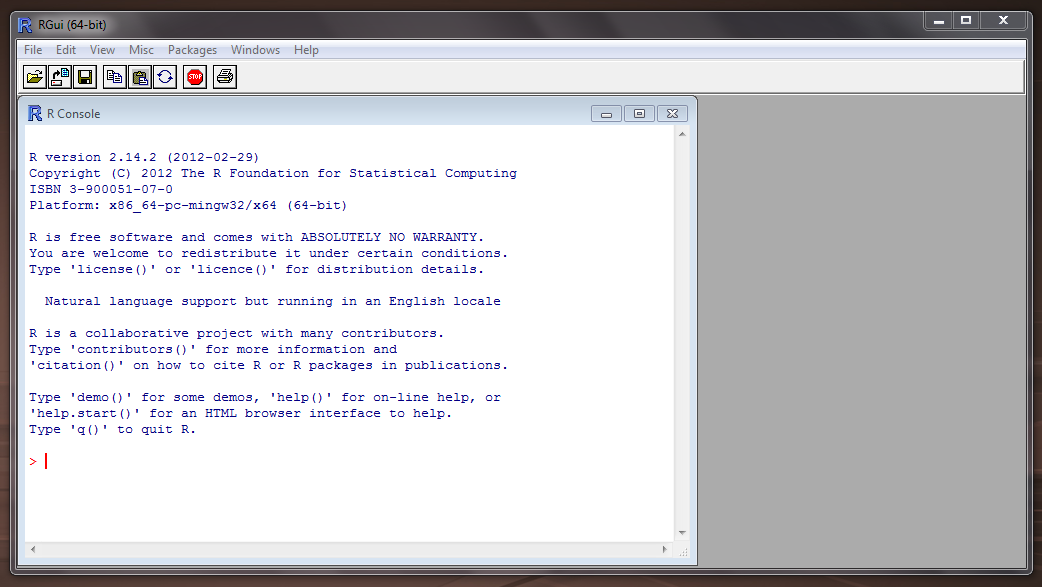
\includegraphics[width=1\linewidth]{images/rgui-windows} \caption{Interface gráfica do usuário no R para Windows.}\label{fig:r-gui}
\end{figure}

\subsubsection{\texorpdfstring{Atualização do no
Windows}{Atualização do  no Windows}}\label{atualizacao-do-no-windows}

Novas versões do R são disponibilizadas em geral com frequência de 5
vezes por ano. Recomenda-se manter o R atualizado, pois as novas versões
incluem
\href{https://cran.r-project.org/bin/windows/base/NEWS.R-3.4.4.html}{aperfeiçoamentos
e a correção de \emph{bugs}}.

As novas versões do vem com os
\href{https://cran.r-project.org/doc/manuals/R-FAQ.html\#Which-add_002don-packages-exist-for-R_003f}{pacotes
padrões do R}. Os demais pacotes instalados pelo usuário na versão
anterior precisam ser reinstalados na nova versão do .

Para atualizar o no Windows, ao invés de baixar o executável a cada nova
versão e repetir o processo da seção anterior, você pode utilizar o
pacote
\href{https://cran.r-project.org/web/packages/installr/index.html}{\textbf{installr}}.
A instalação de pacotes no será vista na seção \ref{install-pck}.

\subsection{Linux}\label{linux}

\subsubsection{Ubuntu}\label{ubuntu}

Há várias formas de instalar o no Ubuntu, mas geralmente a versão
compilada no repositório \emph{default} do Ubuntu não é a última. Se
isso não for problema para você então basta executar:

\begin{Shaded}
\begin{Highlighting}[]
\NormalTok{sudo apt}\OperatorTok{-}\NormalTok{get install r}\OperatorTok{-}\NormalTok{base}
\end{Highlighting}
\end{Shaded}

Entretanto, os pacotes do recém lançados são compilados para última
versão do . Então você pode ter restrições ao uso de pacotes novos, os
quais geralmente incluem o estado da arte de análise de dados. Por esta
razão, abaixo mostra-se como instalar o de forma que seja atualizado
automaticamente pelo sistema.

\subsubsection{R sempre atualizado}\label{r-sempre-atualizado}

Se você quer trabalhar sempre com a última versão estável do , é
possível configurar o Linux Ubuntu para atualizar automaticamente o . O
procedimento de instalação requer senha de superusuário do sistema ou de
privilégios \href{https://en.wikipedia.org/wiki/Sudo}{sudo}. Caso não
tenha, consulte o administrador do sistema.

Ao utilizar distribuições Linux Ubuntu é importante optar por versões
estáveis\footnote{Clique \href{http://releases.ubuntu.com}{aqui} para
  saber mais sobre as versões do Ubuntu.}. As versões de Suporte de
longo prazo (LTS) mais recentes são:

\begin{itemize}
\tightlist
\item
  14.04 (abril de 2014, \emph{codename} \texttt{trusty})
\item
  16.04 (abril de 2016, \emph{codename} \texttt{xenial})
\end{itemize}

A versão mais atual é a R version 3.4.4 (2018-03-15). Para que ele seja
atualizado automaticamente no Ubuntu você precisa adicionar o endereço
do \href{http://cran.r-project.org/mirrors.html}{repósitório do R} mais
próximo de sua região à lista de repositórios do Linux. No exemplo deste
livro, o repositório mais próximo é o da UFPR
(\url{http://cran-r.c3sl.ufpr.br/}).

\paragraph{\texorpdfstring{Incluindo repositório do na Lista de
repositórios do
Ubuntu}{Incluindo repositório do  na Lista de repositórios do Ubuntu}}\label{incluindo-repositorio-do-na-lista-de-repositorios-do-ubuntu}

A lista de repositórios do sistema é armazenada no arquivo
\texttt{/etc/apt/sources.list}. Mas primeiro, você precisa descobrir ou
verificar o nome da versão do sistema operacional. Para isso, você pode
utilizar o seguinte comando\footnote{Se o comando \texttt{lsb\_release}
  não funcionar você precisa instalar o pacote \texttt{lsb-release} no
  sistema. Para isso, digite no terminal Linux
  \texttt{sudo\ apt-get\ install\ lsb-release}.} :

\begin{verbatim}
$ lsb_release --codename | cut -f2
\end{verbatim}

\begin{verbatim}
trusty
\end{verbatim}

Precisamos incluir no arquivo \texttt{sources.list} o espelho do
repositório do R mais próximo. Veja a lista de espelhos de repositórios
do \href{https://cran.r-project.org/mirrors.html}{aqui}. Assim o
gerenciador de pacotes
\href{http://pt.wikipedia.org/wiki/Advanced_Packaging_Tool}{apt}\footnote{o
  gerenciador de pacotes
  \href{http://pt.wikipedia.org/wiki/Advanced_Packaging_Tool}{apt} é
  usado para instalação, atualização e remoção de pacotes em
  distribuições Debian GNU/Linux.} fará a atualização do quando uma nova
versão estiver disponível. Ou seja, você estará utilizando sempre versão
mais atual do .

O endereço do repositório da UFPR será inserido na última linha do
arquivo \texttt{sources.list} usando alguns comandos linux. Essa tarefa
requer privilégios de
\href{https://pt.wikipedia.org/wiki/Superusu\%C3\%A1rio}{superusuário}.
Vamos trocar do seu usuário para o superusuário.

\begin{verbatim}
$ sudo su
\end{verbatim}

Vamos definir no terminal uma variável com o endereço do repositório (da
UFPR nesse caso) e o nome de versão do Ubuntu.

\begin{verbatim}
# repos="deb http://cran-r.c3sl.ufpr.br/bin/linux/ubuntu `lsb_release --codename | cut -f2`/"
\end{verbatim}

Note que a variável \texttt{repos} é uma sequência de caracteres com as
seguintes informações:

\begin{verbatim}
deb `linkRepositorioSelecionado`/bin/linux/ubuntu `versaoUbuntu`/
\end{verbatim}

O valor da variável \texttt{repos} é mostrado pelo comando:
\texttt{echo\ \$repos}. Certifique-se de que a última palavra
corresponde ao nome da sua versão Ubuntu.

Para acrescentar essa informação no final do arquivo
\texttt{sources.list} digite no terminal linux:

\begin{verbatim}
# echo $repos >> /etc/apt/sources.list
\end{verbatim}

Feito isso, você pode retornar a sessão de usuário comum, usando o
comando abaixo:

\begin{verbatim}
# exit
\end{verbatim}

\paragraph{\texorpdfstring{\href{https://cran.r-project.org/bin/linux/ubuntu/README.html\#secure-apt}{APT
protegido}}{APT protegido}}\label{apt-protegido}

Os arquivos binários do para Ubuntu na
\href{http://cran.r-project.org}{CRAN} são assinados com uma chave
pública\footnote{Chave pública de autenticação é um meio alternativo de
  se logar em um servidor ao invés de digitar uma senha. É uma forma
  mais segura e flexível, mas mais difícil de ser configurada. Esse meio
  alternativo de fazer login é importante se o computador está visível
  na internet. Para saber mais veja
  \href{http://the.earth.li/~sgtatham/putty/0.55/htmldoc/Chapter8.html}{aqui}.}
Para adicionar essa chave ao seu sistema digite os seguintes comandos:

\begin{verbatim}
$ gpg --keyserver hkp://keyserver.ubuntu.com:80 --recv-keys E084DAB9
\end{verbatim}

e então use essa informação como entrada no \texttt{apt-key} com

\begin{verbatim}
$ gpg -a --export E084DAB9 | sudo apt-key add -
  
\end{verbatim}

Se aparecer a mensagem de que a chave pública foi importada, então não
há necessidade de executar os comandos abaixo. Mas caso seja impresso
alguma mensagem de erro, outra alternativa pode ser usada para obter a
chave, via os comandos:

\begin{verbatim}
$ gpg --keyserver keyserver.ubuntu.com --recv-key E084DAB9
$ gpg -a --export E084DAB9 | sudo apt-key add -
\end{verbatim}

\paragraph{Atualização da lista de repositórios do Ubuntu e instalação
do
}\label{atualizacao-da-lista-de-repositorios-do-ubuntu-e-instalacao-do}

Após fazer as configurações da lista de repositórios e adicionar a chave
é necessário fazer a atualização dessa lista (requer poderes de super
usuário):

\begin{verbatim}
$ sudo apt-get update
\end{verbatim}

Agora, pode instalar o binário do R:

\begin{verbatim}
$ sudo apt-get install r-base
\end{verbatim}

\paragraph{Testando o }\label{testando-o}

Para iniciar o no Ubuntu, digite \texttt{R} no cursor do terminal:

\begin{verbatim}
$ R
\end{verbatim}

A partir desse momento já começamos uma sessão no . Vamos gerar uma
sequência numérica de 1 a 10 e plotá-la.

\begin{Shaded}
\begin{Highlighting}[]
\OperatorTok{>}\StringTok{ }\DecValTok{1}\OperatorTok{:}\DecValTok{10}
\NormalTok{ [}\DecValTok{1}\NormalTok{]  }\DecValTok{1}  \DecValTok{2}  \DecValTok{3}  \DecValTok{4}  \DecValTok{5}  \DecValTok{6}  \DecValTok{7}  \DecValTok{8}  \DecValTok{9} \DecValTok{10}
\OperatorTok{>}\StringTok{ }\KeywordTok{plot}\NormalTok{(}\DecValTok{1}\OperatorTok{:}\DecValTok{10}\NormalTok{)}
\end{Highlighting}
\end{Shaded}

\begin{figure}

{\centering 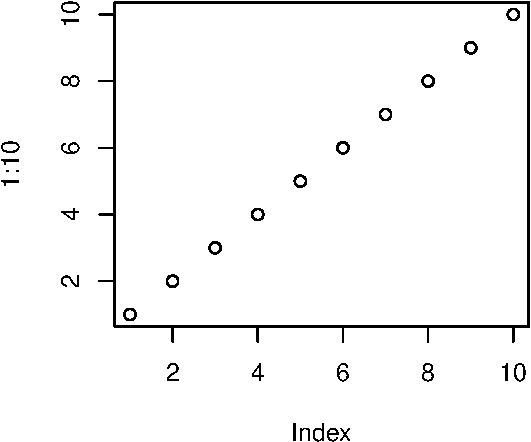
\includegraphics{images/Chunck4-1} 

}

\caption{Gráfico da sequência de 10 números.}\label{fig:Chunck4}
\end{figure}

Você pode sair do , sem salvar os dados da seção, com o código a seguir:

\begin{Shaded}
\begin{Highlighting}[]
\OperatorTok{>}\StringTok{ }\KeywordTok{q}\NormalTok{(}\DataTypeTok{save =} \StringTok{"no"}\NormalTok{)}
\end{Highlighting}
\end{Shaded}

\subsubsection{Diretório para instalação de
pacotes}\label{diretorio-para-instalacao-de-pacotes}

Uma boa prática é definir um diretório para armazenamento dos pacotes
utilizados. Isso lhe dá mais controle sobre os pacotes do instalados no
sistema. Um local sugerido é o \texttt{/home/usuario/.R/libs}. O seu
\texttt{home} ou \texttt{pasta\ pessoal} pode ser obtido com o comando
\texttt{echo\ \$HOME}. Para criar o diretório você pode digitar o
comando abaixo:

\begin{verbatim}
$ mkdir -p `echo $HOME`/.R/libs/
\end{verbatim}

Para informar ao onde procurar os pacotes instalados, você precisa criar
um arquivo chamado \texttt{.Renviron}, no diretório \texttt{\$HOME},
contendo a expressão \texttt{R\_LIBS=/home/usuario/.R/libs/}. Você pode
fazer isso em um terminal com os comandos:

\begin{verbatim}
$ R_LIBS=`echo $HOME/.R/libs/`
$ echo $R_LIBS >> `echo $HOME/.Renviron`
\end{verbatim}

Esse caminho fica então visível ao , o que pode ser verificado
executando a função \texttt{.libPaths()} na linha de comando do .

Abra o :

\begin{verbatim}
$ R
\end{verbatim}

e ao digitar:

\begin{Shaded}
\begin{Highlighting}[]
\OperatorTok{>}\StringTok{ }\KeywordTok{.libPaths}\NormalTok{()}
\NormalTok{[}\DecValTok{1}\NormalTok{] }\StringTok{"/home/hidrometeorologista/.R/libs"} \StringTok{"/usr/local/lib/R/site-library"}    
\NormalTok{[}\DecValTok{3}\NormalTok{] }\StringTok{"/usr/lib/R/site-library"}           \StringTok{"/usr/lib/R/library"}               
\end{Highlighting}
\end{Shaded}

o seu diretório \texttt{/home/usuario/.R/libs}\footnote{Diretórios
  precedidos por ``.'' no Linux são diretórios ocultos. O diretório
  \texttt{/home/usuario/.R} é um diretório oculto, para visualizá-lo no
  Ubuntu, na interface gráfica do sistema, acesse \emph{View
  \textgreater{} Show Hidden Files} (ou \emph{Visualizar \textgreater{}
  Mostrar arquivos ocultos}). No terminal utilize \texttt{ls\ -a} para
  listar os arquivos ocultos.} deve aparecer em primeiro lugar.
Indicando que este local tem prioridade para instalação dos pacotes.
Caso o diretório deixe de existir os seguintes diretórios serão usados.

\section{Pacotes do R}\label{install-pck}

\subsection{Da internet}\label{da-internet}

\subsubsection{CRAN}\label{cran}

A forma mais fácil de instalar uma pacote do R é através da função
\texttt{install.packages("nome\_do\_pacote")}.

Por \emph{default} o pacote informado é instalado a partir da
(\href{https://cran.r-project.org/}{CRAN})

Por exemplo, para instalar o pacote \textbf{devtools}:

\begin{Shaded}
\begin{Highlighting}[]
\KeywordTok{install.packages}\NormalTok{(}\StringTok{"devtools"}\NormalTok{)}
\end{Highlighting}
\end{Shaded}

A função automaticamente resolverá as dependências do pacote, de forma
que qualquer pacote dependente também será instalado.

Para ter acesso as funções disponibilizadas com o pacote você precisa
carregar o pacote:

\begin{Shaded}
\begin{Highlighting}[]
\KeywordTok{library}\NormalTok{(devtools)}
\end{Highlighting}
\end{Shaded}

Para desinstalar um pacote você pode usar a função
\texttt{remove.packages("nome\_do\_pacote")}.

\subsubsection{GitHub e R-forge}\label{github-e-r-forge}

Nem todos pacotes são disponíveis na CRAN. Muitos desenvolvedores
disponibilizam seus pacotes em plataormas como o
\href{https://github.com/}{GitHub} e
\href{https://r-forge.r-project.org/}{R-forge}. As vezes um pacote pode
estar em ambos CRAN e GitHub (ou R-forge), mas a última versão - a de
desenvolvimento - é somente disponibilizada no GitHub (ou R-forge).

Para instalar um pacote de um repositório do GitHub usa-se a função
\texttt{install\_github()} do pacote \textbf{devtools}. Portanto, o
pacote \textbf{devtools} precisa ser instalado primeiro.

Antes de instalar o pacote \textbf{devtools}, usuários Windows precisam
instalar o programa
\href{https://cran.r-project.org/bin/windows/Rtools/index.html}{Rtools}.

A função para instalar um pacote do GitHub requer como argumento o nome
do usuário e do repositório. Por exemplo, para instalar o pacote
\texttt{inmetr} do repositório mantido pelo autor deste livro, usa-se:

\begin{Shaded}
\begin{Highlighting}[]
\CommentTok{# install.packages("devtools")}
\CommentTok{# carrega o pacote devtools}
\KeywordTok{library}\NormalTok{(devtools)}
\CommentTok{# instala o pacote inmetr do repositório }
\CommentTok{# https://github.com/lhmet/inmetr }
\KeywordTok{install_github}\NormalTok{(}\StringTok{"lhmet/inmetr"}\NormalTok{)}
\end{Highlighting}
\end{Shaded}

Para um repositório do R-forge, por exemplo o repositório do pacote
\href{https://r-forge.r-project.org/projects/raster/}{raster}, usa-se:

\begin{Shaded}
\begin{Highlighting}[]
\KeywordTok{install.packages}\NormalTok{(}\StringTok{"raster"}\NormalTok{, }\DataTypeTok{repos =} \StringTok{"http://R-Forge.R-project.org"}\NormalTok{)}
\end{Highlighting}
\end{Shaded}

\subsubsection{Arquivo fonte local}\label{arquivo-fonte-local}

Códigos fonte de pacotes do R são armazenados como arquivos com a
extensão \texttt{.tar.gz}. Binários compilados são armazenados com a
extensão \texttt{.zip}. Exemplo de arquivos como estes podem ser
baixados manualmente da CRAN (veja a seção Downloads em
\url{https://cran.r-project.org/web/packages/ggplot2/index.html}),
GitHub ou R-forge.

Eventualmente um usuário pode instalar um pacote a partir desses
arquivos localmente. Isto pode também ser feito com a função
\texttt{install.packages()}, especifincando o argumento
\texttt{repos\ =\ NULL} e o argumento \texttt{pkgs} com o caminho do
arquivo. Por exemplo:

\begin{Shaded}
\begin{Highlighting}[]
\KeywordTok{install.packages}\NormalTok{(}\StringTok{"ggplot2_2.1.0.tar.gz"}\NormalTok{, }\DataTypeTok{repos=}\OtherTok{NULL}\NormalTok{)}
\end{Highlighting}
\end{Shaded}

\section{RStudio no Ubuntu}\label{install-rstudio}

 é uma empresa que desenvolve ferramentas gratuitas para o e
\href{https://www.rstudio.com/products/}{produtos pagos} para empresas.

Uma de suas ferramentas gratuitas é o software RStudio \emph{Desktop}
que consiste em um ambiente integrado de desenvolvimento
(\href{http://en.wikipedia.org/wiki/Integrated_development_environment}{IDE})
construído especificamente para o , consequentemente, também é
multiplataforma.

Para instalação da versão do RStudio para
\emph{\href{https://pt.wikipedia.org/wiki/Ambiente_de_desktop}{Desktop}},
você precisa saber se seu SO é 64 ou 32-bit e a versão do Linux Ubuntu.
Essas informações podem ser obtidas, respectivamente, pelos comandos:

\begin{verbatim}
$ arch
\end{verbatim}

\begin{verbatim}
x86_64
\end{verbatim}

Se retornar \textbf{x86\_64} sua máquina é 64-bit.

\begin{verbatim}
$ lsb_release --release | cut -f2
\end{verbatim}

\begin{verbatim}
14.04
\end{verbatim}

Com essas informações, siga os seguintes passos:

\begin{enumerate}
\def\labelenumi{\arabic{enumi}.}
\tightlist
\item
  acesse
  \href{https://www.rstudio.com/products/rstudio/download/}{RStudio}
\item
  clique em \emph{Download} (Figura \ref{fig:rstudio-choose})
\end{enumerate}

\begin{figure}

{\centering 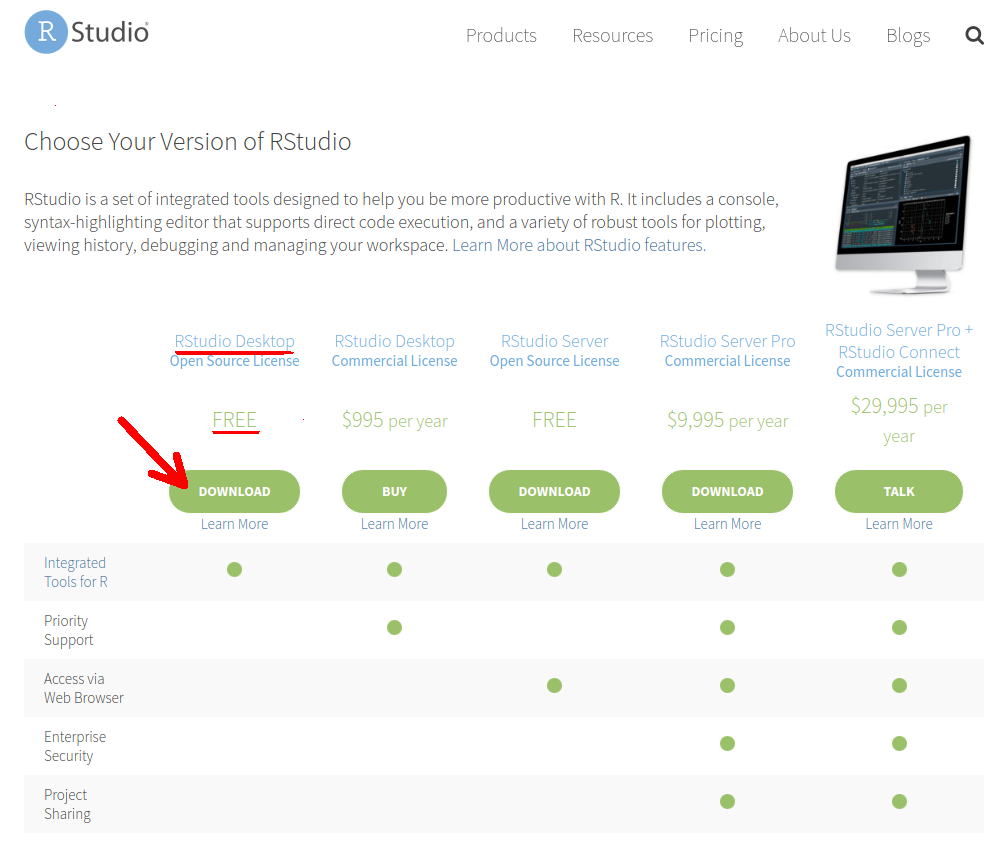
\includegraphics[width=1\linewidth]{images/rstudio-choose} 

}

\caption{Opção para baixar o RStudio *Desktop*.}\label{fig:rstudio-choose}
\end{figure}

\begin{enumerate}
\def\labelenumi{\arabic{enumi}.}
\setcounter{enumi}{2}
\tightlist
\item
  Clique na sua plataforma (de acordo com seu SO, arquitetura e versão
  da distribuição) (Figura \ref{fig:rstudio-plat}), no exemplo deste
  livro \emph{RStudio 1.1.447 - Ubuntu 12.04-15.10/Debian 8 (64-bit)}
\end{enumerate}

\begin{figure}

{\centering 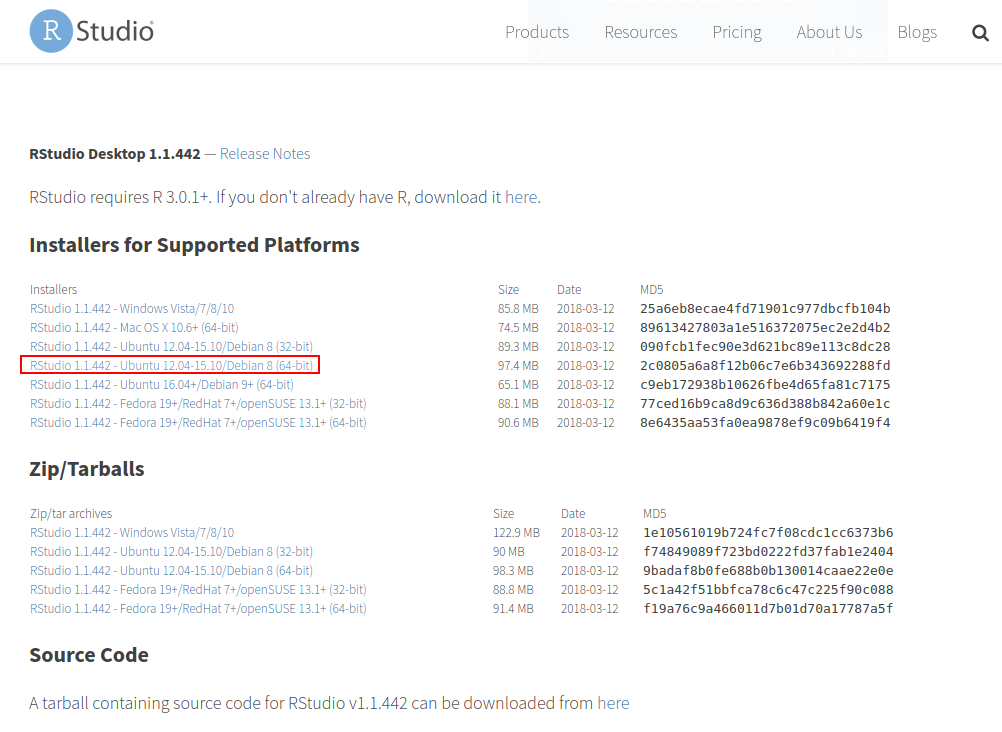
\includegraphics[width=1\linewidth]{images/rstudio-plataform-options} 

}

\caption{Escolha da plataforma em que será o usada o RStudio *Desktop*.}\label{fig:rstudio-plat}
\end{figure}

\begin{enumerate}
\def\labelenumi{\arabic{enumi}.}
\setcounter{enumi}{3}
\tightlist
\item
  Dependendo da sua versão Ubuntu, ao clicar sobre o sobre o arquivo
  baixado com o botão direito, há a opção de abrir com \emph{Ubuntu
  Software Center} e então clicar em \texttt{instalar}. Se na versão de
  seu \emph{Desktop} não há esta opção ao clicar com botão direito sobre
  o arquivo, instale via \textbf{terminal}\footnote{digite `Ctrl+Alt+t'
    para abrir um terminal no Linux Ubuntu} com os seguintes comandos:
\end{enumerate}

\begin{verbatim}
$ cd /local/do/arquivo/baixado
$ sudo dpkg -i arquivoBaixado.deb
$ sudo apt-get install -f
\end{verbatim}

Abra o RStudio digitando no terminal:

\begin{verbatim}
$ rstudio &
\end{verbatim}

Agora você está pronto para começar a programar em aproveitando as
facilidades que o \href{http://www.rstudio.com/}{RStudio} oferece.

\chapter{Interface do Usuário}\label{iu}

Na maior parte do tempo você provavelmente usará o no \textbf{modo
interativo}: rodando comandos e vendo os resultados.

Eventualmente esse processo pode ser inconveniente. Por exemplo, no caso
de uma análise com um código bem extenso e que precisa ser repetida com
dados atualizados semanalmente. Nessa situação, recomenda-se a criação
de um script, ou seja, um arquivo texto, com a extensão \texttt{.R},
contendo o código de sua análise.

Esse \emph{script} pode ser executado pelo R no \textbf{modo de
processamento em lote} (do termo em inglês \emph{Batch Processing})
através de um terminal do SO Linux, ou via o Prompt de comando
(\texttt{cmd.exe}) do SO Windows.

Nesta seção apresenta-se ao leitor estes dois modos de execução do .

\section{ no modo interativo}\label{no-modo-interativo}

No Linux o pode ser aberto simplesmente digitando em um terminal a letra
\texttt{R}.

\begin{Shaded}
\begin{Highlighting}[]
\NormalTok{$ }\ExtensionTok{R}
\end{Highlighting}
\end{Shaded}

\begin{verbatim}
R version 3.4.4 (2018-03-15) -- "Someone to Lean On"
Copyright (C) 2018 The R Foundation for Statistical Computing
Platform: x86_64-pc-linux-gnu (64-bit)

R is free software and comes with ABSOLUTELY NO WARRANTY.
You are welcome to redistribute it under certain conditions.
Type 'license()' or 'licence()' for distribution details.

  Natural language support but running in an English locale

R is a collaborative project with many contributors.
Type 'contributors()' for more information and
'citation()' on how to cite R or R packages in publications.

Type 'demo()' for some demos, 'help()' for on-line help, or
'help.start()' for an HTML browser interface to help.
Type 'q()' to quit R.

> 
\end{verbatim}

A janela com a linha de comando do apresenta o \emph{prompt} do
(\texttt{\textgreater{}}). Após este símbolo digitamos os comandos,
pressionamos a tecla \texttt{\textless{}enter\textgreater{}}, o
interpreta o comando e retorna o resultado.

Os comandos digitados na linha de comando são chamados de expressões.
Esse é o modo iterativo do . Portanto, a linha de comando é a mais
importante ferramenta do , pois todas expressões são avaliadas através
dela.

\begin{Shaded}
\begin{Highlighting}[]
\OperatorTok{>}\StringTok{ }\DecValTok{62} \OperatorTok{+}\StringTok{ }\DecValTok{38}
\NormalTok{[}\DecValTok{1}\NormalTok{] }\DecValTok{100}
\end{Highlighting}
\end{Shaded}

A expressão é avaliada pelo , o resultado é mostrado, mas o seu valor é
perdido.

O número entre colchetes que aparece como resultado da operação
(``{[}1{]}'' no caso acima) indica o conteúdo resultante da operação
iniciando na posição 1 desse objeto. O significado dessa informação
torna-se mais óbvio quando trabalhamos com objetos maiores, como por
exemplo com vetores. Observe os valores nos colchetes para uma sequência
de 100 até 1.

\begin{Shaded}
\begin{Highlighting}[]
\OperatorTok{>}\StringTok{ }\DecValTok{100}\OperatorTok{:}\DecValTok{1}
\NormalTok{  [}\DecValTok{1}\NormalTok{] }\DecValTok{100}  \DecValTok{99}  \DecValTok{98}  \DecValTok{97}  \DecValTok{96}  \DecValTok{95}  \DecValTok{94}  \DecValTok{93}  \DecValTok{92}  \DecValTok{91}  \DecValTok{90}  \DecValTok{89}  \DecValTok{88}  \DecValTok{87}  \DecValTok{86}  \DecValTok{85}  \DecValTok{84}
\NormalTok{ [}\DecValTok{18}\NormalTok{]  }\DecValTok{83}  \DecValTok{82}  \DecValTok{81}  \DecValTok{80}  \DecValTok{79}  \DecValTok{78}  \DecValTok{77}  \DecValTok{76}  \DecValTok{75}  \DecValTok{74}  \DecValTok{73}  \DecValTok{72}  \DecValTok{71}  \DecValTok{70}  \DecValTok{69}  \DecValTok{68}  \DecValTok{67}
\NormalTok{ [}\DecValTok{35}\NormalTok{]  }\DecValTok{66}  \DecValTok{65}  \DecValTok{64}  \DecValTok{63}  \DecValTok{62}  \DecValTok{61}  \DecValTok{60}  \DecValTok{59}  \DecValTok{58}  \DecValTok{57}  \DecValTok{56}  \DecValTok{55}  \DecValTok{54}  \DecValTok{53}  \DecValTok{52}  \DecValTok{51}  \DecValTok{50}
\NormalTok{ [}\DecValTok{52}\NormalTok{]  }\DecValTok{49}  \DecValTok{48}  \DecValTok{47}  \DecValTok{46}  \DecValTok{45}  \DecValTok{44}  \DecValTok{43}  \DecValTok{42}  \DecValTok{41}  \DecValTok{40}  \DecValTok{39}  \DecValTok{38}  \DecValTok{37}  \DecValTok{36}  \DecValTok{35}  \DecValTok{34}  \DecValTok{33}
\NormalTok{ [}\DecValTok{69}\NormalTok{]  }\DecValTok{32}  \DecValTok{31}  \DecValTok{30}  \DecValTok{29}  \DecValTok{28}  \DecValTok{27}  \DecValTok{26}  \DecValTok{25}  \DecValTok{24}  \DecValTok{23}  \DecValTok{22}  \DecValTok{21}  \DecValTok{20}  \DecValTok{19}  \DecValTok{18}  \DecValTok{17}  \DecValTok{16}
\NormalTok{ [}\DecValTok{86}\NormalTok{]  }\DecValTok{15}  \DecValTok{14}  \DecValTok{13}  \DecValTok{12}  \DecValTok{11}  \DecValTok{10}   \DecValTok{9}   \DecValTok{8}   \DecValTok{7}   \DecValTok{6}   \DecValTok{5}   \DecValTok{4}   \DecValTok{3}   \DecValTok{2}   \DecValTok{1}
\end{Highlighting}
\end{Shaded}

O elemento \texttt{{[}18{]}} da sequência de 100 até 1 é o número
\texttt{83}.

Pode ocorrer da expressão digitada na linha ser muito extensa e ir além
de uma linha. Se a expressão estiver incompleta o mostra um sinal de
\texttt{+}.

\begin{Shaded}
\begin{Highlighting}[]
\OperatorTok{>}\StringTok{ }\DecValTok{1} \OperatorTok{*}\StringTok{ }\DecValTok{2} \OperatorTok{*}\StringTok{ }\DecValTok{3} \OperatorTok{*}\StringTok{ }\DecValTok{4} \OperatorTok{*}\StringTok{ }\DecValTok{5} \OperatorTok{*}
\OperatorTok{+}\StringTok{ }\DecValTok{6} \OperatorTok{*}\StringTok{ }\DecValTok{7} \OperatorTok{*}\StringTok{ }\DecValTok{8} \OperatorTok{*}\StringTok{ }\DecValTok{9} \OperatorTok{*}\StringTok{ }\DecValTok{10}
\NormalTok{[}\DecValTok{1}\NormalTok{] }\DecValTok{3628800}
\end{Highlighting}
\end{Shaded}

Execute a expressão abaixo até o sinal de menos e tecle
\texttt{\textless{}enter\textgreater{}}. Enquanto a expressão não
estiver completa o sinal de + se repetirá. Até que você digite o número
que deseja subtrair de 4.

\begin{Shaded}
\begin{Highlighting}[]
\OperatorTok{>}\StringTok{ }\DecValTok{4} \OperatorTok{-}
\OperatorTok{+}\StringTok{   }
\OperatorTok{+}\StringTok{   }\DecValTok{3}
\NormalTok{[}\DecValTok{1}\NormalTok{] }\DecValTok{1}
\end{Highlighting}
\end{Shaded}

\subsection{Expressões em sequência}\label{expressInSeq}

Podemos executar todas expressões anteriores em apenas uma linha, usando
o ponto e vírgula \texttt{;} para separar as expressões:

\begin{Shaded}
\begin{Highlighting}[]
\OperatorTok{>}\StringTok{ }\DecValTok{62} \OperatorTok{+}\StringTok{ }\DecValTok{38}\NormalTok{; }\DecValTok{100}\OperatorTok{:}\DecValTok{1}\NormalTok{; }\DecValTok{1} \OperatorTok{*}\StringTok{ }\DecValTok{2} \OperatorTok{*}\StringTok{ }\DecValTok{3} \OperatorTok{*}\StringTok{ }\DecValTok{4} \OperatorTok{*}\StringTok{ }\DecValTok{5} \OperatorTok{*}\StringTok{ }\DecValTok{6} \OperatorTok{*}\StringTok{ }\DecValTok{7} \OperatorTok{*}\StringTok{ }\DecValTok{8} \OperatorTok{*}\StringTok{ }\DecValTok{9} \OperatorTok{*}\StringTok{ }\DecValTok{10}\NormalTok{; }\DecValTok{4} \OperatorTok{-}\StringTok{ }\DecValTok{3}
\NormalTok{[}\DecValTok{1}\NormalTok{] }\DecValTok{100}
\NormalTok{  [}\DecValTok{1}\NormalTok{] }\DecValTok{100}  \DecValTok{99}  \DecValTok{98}  \DecValTok{97}  \DecValTok{96}  \DecValTok{95}  \DecValTok{94}  \DecValTok{93}  \DecValTok{92}  \DecValTok{91}  \DecValTok{90}  \DecValTok{89}  \DecValTok{88}  \DecValTok{87}  \DecValTok{86}  \DecValTok{85}  \DecValTok{84}
\NormalTok{ [}\DecValTok{18}\NormalTok{]  }\DecValTok{83}  \DecValTok{82}  \DecValTok{81}  \DecValTok{80}  \DecValTok{79}  \DecValTok{78}  \DecValTok{77}  \DecValTok{76}  \DecValTok{75}  \DecValTok{74}  \DecValTok{73}  \DecValTok{72}  \DecValTok{71}  \DecValTok{70}  \DecValTok{69}  \DecValTok{68}  \DecValTok{67}
\NormalTok{ [}\DecValTok{35}\NormalTok{]  }\DecValTok{66}  \DecValTok{65}  \DecValTok{64}  \DecValTok{63}  \DecValTok{62}  \DecValTok{61}  \DecValTok{60}  \DecValTok{59}  \DecValTok{58}  \DecValTok{57}  \DecValTok{56}  \DecValTok{55}  \DecValTok{54}  \DecValTok{53}  \DecValTok{52}  \DecValTok{51}  \DecValTok{50}
\NormalTok{ [}\DecValTok{52}\NormalTok{]  }\DecValTok{49}  \DecValTok{48}  \DecValTok{47}  \DecValTok{46}  \DecValTok{45}  \DecValTok{44}  \DecValTok{43}  \DecValTok{42}  \DecValTok{41}  \DecValTok{40}  \DecValTok{39}  \DecValTok{38}  \DecValTok{37}  \DecValTok{36}  \DecValTok{35}  \DecValTok{34}  \DecValTok{33}
\NormalTok{ [}\DecValTok{69}\NormalTok{]  }\DecValTok{32}  \DecValTok{31}  \DecValTok{30}  \DecValTok{29}  \DecValTok{28}  \DecValTok{27}  \DecValTok{26}  \DecValTok{25}  \DecValTok{24}  \DecValTok{23}  \DecValTok{22}  \DecValTok{21}  \DecValTok{20}  \DecValTok{19}  \DecValTok{18}  \DecValTok{17}  \DecValTok{16}
\NormalTok{ [}\DecValTok{86}\NormalTok{]  }\DecValTok{15}  \DecValTok{14}  \DecValTok{13}  \DecValTok{12}  \DecValTok{11}  \DecValTok{10}   \DecValTok{9}   \DecValTok{8}   \DecValTok{7}   \DecValTok{6}   \DecValTok{5}   \DecValTok{4}   \DecValTok{3}   \DecValTok{2}   \DecValTok{1}
\NormalTok{[}\DecValTok{1}\NormalTok{] }\DecValTok{3628800}
\NormalTok{[}\DecValTok{1}\NormalTok{] }\DecValTok{1}
\end{Highlighting}
\end{Shaded}

\subsection{Navegação entre as expressões já
avaliadas}\label{navegacao-entre-as-expressoes-ja-avaliadas}

Você pode usar as teclas ⬆️ e ⬇️ para navegar entre as expressões já
avaliadas pelo . O que é útil quando precisamos repetir um comando
anterior com alguma mudança ou para corrigir um erro de digitação ou a
omissão de um parentêses.

Quando a linha de comando é usada por muito tempo a sua tela pode ficar
poluída com a saída das expressões anteriores. Para limpar a tela, tecle
\texttt{Ctrl+l}. Assim o console aparece na parte superior do terminal.

\begin{Shaded}
\begin{Highlighting}[]
\OperatorTok{>}\StringTok{ }\DecValTok{15} \OperatorTok{+}\StringTok{ }\DecValTok{4}
\NormalTok{[}\DecValTok{1}\NormalTok{] }\DecValTok{19}
\OperatorTok{>}\StringTok{ }\DecValTok{100}\OperatorTok{:}\DecValTok{1}
\NormalTok{  [}\DecValTok{1}\NormalTok{] }\DecValTok{100}  \DecValTok{99}  \DecValTok{98}  \DecValTok{97}  \DecValTok{96}  \DecValTok{95}  \DecValTok{94}  \DecValTok{93}  \DecValTok{92}  \DecValTok{91}  \DecValTok{90}  \DecValTok{89}  \DecValTok{88}  \DecValTok{87}  \DecValTok{86}  \DecValTok{85}  \DecValTok{84}
\NormalTok{ [}\DecValTok{18}\NormalTok{]  }\DecValTok{83}  \DecValTok{82}  \DecValTok{81}  \DecValTok{80}  \DecValTok{79}  \DecValTok{78}  \DecValTok{77}  \DecValTok{76}  \DecValTok{75}  \DecValTok{74}  \DecValTok{73}  \DecValTok{72}  \DecValTok{71}  \DecValTok{70}  \DecValTok{69}  \DecValTok{68}  \DecValTok{67}
\NormalTok{ [}\DecValTok{35}\NormalTok{]  }\DecValTok{66}  \DecValTok{65}  \DecValTok{64}  \DecValTok{63}  \DecValTok{62}  \DecValTok{61}  \DecValTok{60}  \DecValTok{59}  \DecValTok{58}  \DecValTok{57}  \DecValTok{56}  \DecValTok{55}  \DecValTok{54}  \DecValTok{53}  \DecValTok{52}  \DecValTok{51}  \DecValTok{50}
\NormalTok{ [}\DecValTok{52}\NormalTok{]  }\DecValTok{49}  \DecValTok{48}  \DecValTok{47}  \DecValTok{46}  \DecValTok{45}  \DecValTok{44}  \DecValTok{43}  \DecValTok{42}  \DecValTok{41}  \DecValTok{40}  \DecValTok{39}  \DecValTok{38}  \DecValTok{37}  \DecValTok{36}  \DecValTok{35}  \DecValTok{34}  \DecValTok{33}
\NormalTok{ [}\DecValTok{69}\NormalTok{]  }\DecValTok{32}  \DecValTok{31}  \DecValTok{30}  \DecValTok{29}  \DecValTok{28}  \DecValTok{27}  \DecValTok{26}  \DecValTok{25}  \DecValTok{24}  \DecValTok{23}  \DecValTok{22}  \DecValTok{21}  \DecValTok{20}  \DecValTok{19}  \DecValTok{18}  \DecValTok{17}  \DecValTok{16}
\NormalTok{ [}\DecValTok{86}\NormalTok{]  }\DecValTok{15}  \DecValTok{14}  \DecValTok{13}  \DecValTok{12}  \DecValTok{11}  \DecValTok{10}   \DecValTok{9}   \DecValTok{8}   \DecValTok{7}   \DecValTok{6}   \DecValTok{5}   \DecValTok{4}   \DecValTok{3}   \DecValTok{2}   \DecValTok{1}
\OperatorTok{>}\StringTok{ }\CommentTok{#tecle <Ctr + l>}
\end{Highlighting}
\end{Shaded}

Para parar ou cancelar a execução de uma expressão utilize as teclas
\texttt{Ctrl\ +\ C}. As teclas \texttt{Ctrl\ +\ l} tem o efeito de
limpar a tela.

\subsection{Comentários}\label{comentarios}

No , a cerquilha \texttt{\#} (hashtag) é um caracter especial. Qualquer
coisa após esse caracter será ignorada pelo . Somente as expressões
antes da \texttt{\#} são avaliadas. Por meio desse símbolo de comentário
podemos fazer anotações e comentários no código sem atrapalhar a
interpretação das expressões pelo .

\begin{Shaded}
\begin{Highlighting}[]
\OperatorTok{>}\StringTok{ }\CommentTok{# comentário antes do código }
\end{Highlighting}
\end{Shaded}

\begin{Shaded}
\begin{Highlighting}[]
\OperatorTok{>}\StringTok{ }\DecValTok{17} \OperatorTok{+}\StringTok{ }\DecValTok{3} \CommentTok{# comentário ao lado do código: adicionando 17 e 3}
\NormalTok{[}\DecValTok{1}\NormalTok{] }\DecValTok{20}
\end{Highlighting}
\end{Shaded}

\subsection{Auto preenchimento de
funções}\label{auto-preenchimento-de-funcoes}

O inclui o preenchimento automático de nomes de funções e arquivos por
meio da tecla \texttt{\textless{}tab\textgreater{}}. Uma lista de
possíveis funções que começam com as letras inicialmente digitadas
aparecerão.

\begin{Shaded}
\begin{Highlighting}[]
\OperatorTok{>}\StringTok{ }\NormalTok{read}\CommentTok{#<tab> pressione <tab> para ver as opções de comandos que iniciam com o termo read}
\end{Highlighting}
\end{Shaded}

\subsection{\texorpdfstring{Primeiro
\emph{script}}{Primeiro script}}\label{primeiro-script}

O trecho de código abaixo apresenta nas primeiras linhas algumas
expressões do executadas anteriormente. Mas há também, na segunda parte,
códigos para salvar um gráfico de pontos num arquivo \emph{pdf}. Na
última parte do trecho, define-se uma variável \texttt{x} que contém
aquela mesma sequência numérica usada no gráfico.

\begin{Shaded}
\begin{Highlighting}[]
\CommentTok{# Primeiro script no R}
\CommentTok{#----------------------------------------------------------------}
\CommentTok{# cálculos básicos}
\DecValTok{15} \OperatorTok{+}\StringTok{ }\DecValTok{4}
\DecValTok{1}\OperatorTok{:}\DecValTok{100}
\DecValTok{1} \OperatorTok{*}\StringTok{ }\DecValTok{2} \OperatorTok{*}\StringTok{ }\DecValTok{3} \OperatorTok{*}\StringTok{ }\DecValTok{4} \OperatorTok{*}\StringTok{ }\DecValTok{5} \OperatorTok{*}\DecValTok{6} \OperatorTok{*}\StringTok{ }\DecValTok{7} \OperatorTok{*}\StringTok{ }\DecValTok{8} \OperatorTok{*}\StringTok{ }\DecValTok{9} \OperatorTok{*}\StringTok{ }\DecValTok{10}
\DecValTok{4}\OperatorTok{-}\DecValTok{3}
\CommentTok{#----------------------------------------------------------------}
\CommentTok{# salvando um gráfico em um arquivo pdf}
\NormalTok{arquivo_pdf <-}\StringTok{ "plot-script1.pdf"}
\KeywordTok{pdf}\NormalTok{(arquivo_pdf)        }\CommentTok{# cria e abre um arquivo pdf}
\KeywordTok{plot}\NormalTok{(}\DecValTok{1}\OperatorTok{:}\DecValTok{100}\NormalTok{)             }\CommentTok{# faz o gráfico}
\KeywordTok{dev.off}\NormalTok{()               }\CommentTok{# fecha o arquivo pdf}
\CommentTok{#----------------------------------------------------------------}
\CommentTok{# definindo uma variável x}
\NormalTok{x <-}\StringTok{ }\DecValTok{1}\OperatorTok{:}\DecValTok{100}
\NormalTok{x}
\end{Highlighting}
\end{Shaded}

Este conjunto de linhas de código, quando inseridos em um arquivo
texto\footnote{Para fazer isso, você pode usar um editor de texto
  qualquer (p.ex.:
  \href{https://help.gnome.org/users/gedit/stable/index.html.pt_BR}{gedit}
  no SO Linux, ou
  \href{https://pt.wikipedia.org/wiki/Bloco_de_Notas}{Notepad} no SO
  Windows).} formam um primeiro \emph{script} . Este \emph{script} pode
ser executado pelo através da função \texttt{source()}, usando como
argumento o caminho para o local do \emph{script}.

\begin{Shaded}
\begin{Highlighting}[]
\OperatorTok{>}\StringTok{ }\KeywordTok{source}\NormalTok{(}\StringTok{"/home/usuario/adar/script1.R"}\NormalTok{)}
\end{Highlighting}
\end{Shaded}

Este \emph{script} produzirá como saída o arquivo
\texttt{/home/usuario/adar/plot-script1.pdf}. Você pode visualizar o
arquivo para conferir o gráficos de pontos gerado.

\section{ no modo de processamento em
lote}\label{no-modo-de-processamento-em-lote}

Para rodar um \emph{script} no modo de processamento em lote do através
do seguinte comando no terminal Linux:

\begin{verbatim}
$ R CMD BATCH opcoes arqentrada arqsaida
\end{verbatim}

Onde: \texttt{arqentrada}é o nome do script (arquivo com a extensão
\texttt{.R}) a ser executado; \texttt{arqsaida} é o arquivo (com a
extensão \texttt{.Rout}) com as saídas dos comandos executados no R;
\texttt{opcoes} é a lista de opções que controlam a execução.

Vamos rodar como exemplo, o \texttt{script1.R} da seção
\ref{primeiro-script}.

\begin{verbatim}
$ R CMD BATCH /home/usuario/adar/script1.R
\end{verbatim}

O comando acima, produzirá dois arquivos de saída:

\begin{enumerate}
\def\labelenumi{\arabic{enumi}.}
\tightlist
\item
  \texttt{script1.Rout}\footnote{Você pode notar que este arquivo tem o
    mesmo nome do \texttt{arqentrada}, exceto que a sua extensão foi
    alterada para \texttt{.Rout}.} criado por \emph{default} quando o
  \texttt{arqsaida} não é especificado, e;
\end{enumerate}

\begin{enumerate}
\def\labelenumi{\arabic{enumi}.}
\setcounter{enumi}{1}
\tightlist
\item
  arquivo "plot-script1.pdf".
\end{enumerate}

Você pode especificar o nome do \texttt{arqsaida} como desejar. No
exemplo abaixo, mostra-se como salvar o arquivo de saída incluindo a
data em que ele foi gerado, \texttt{script1-saida-adatadehoje.log}.

\begin{verbatim}
$ R CMD BATCH script1.R script1-saida-`date "+%Y%m%d"`.log
\end{verbatim}

Após a execução do último comando, os mesmos arquivos resultantes do
comando anterior serão gerados, exceto pelo primeiro (\texttt{.Rout}),
que será nomeado \texttt{script1-saida-20180507.Rout}.

Para mais opções do comando \texttt{R\ CMD\ BATCH} digite no terminal do
Linux \texttt{R\ -\/-help}.

\chapter{RStudio}\label{rstudio}

O RStudio \emph{Desktop} é um ambiente integrado de desenvolvimento
(IDE) para o . Portanto, o RStudio depende da instalação prévia do . Ele
funciona como uma interface gráfica do usuário (GUI), mas com muito mais
potencialidades.

O RStudio é uma ferramente que potencializará sua interação com o :

\begin{itemize}
\item
  na produção de gráficos
\item
  na organização de seu código na forma de projetos
\item
  na reprodutibilidade de seu trabalho ou pesquisa
\item
  na manutenção e criação de seus próprios pacotes do R
\item
  na criação e compartilhamento de seus relatórios
\item
  no compartilhamento de seu código e a colaboração com outros
\end{itemize}

Nessa seção você terá uma visão geral do RStudio \emph{Desktop}.

\section{Visão geral do RStudio}\label{visao-geral-do-rstudio}

Assumindo que o RStudio tenha sido instalado (seção
\ref{install-rstudio}), ao abri-lo e clicar em \emph{File \textgreater{}
New File \textgreater{} R script} você verá uma tela com aspecto similar
ao da Figura \ref{fig:rstudio-fig}.

\begin{figure}
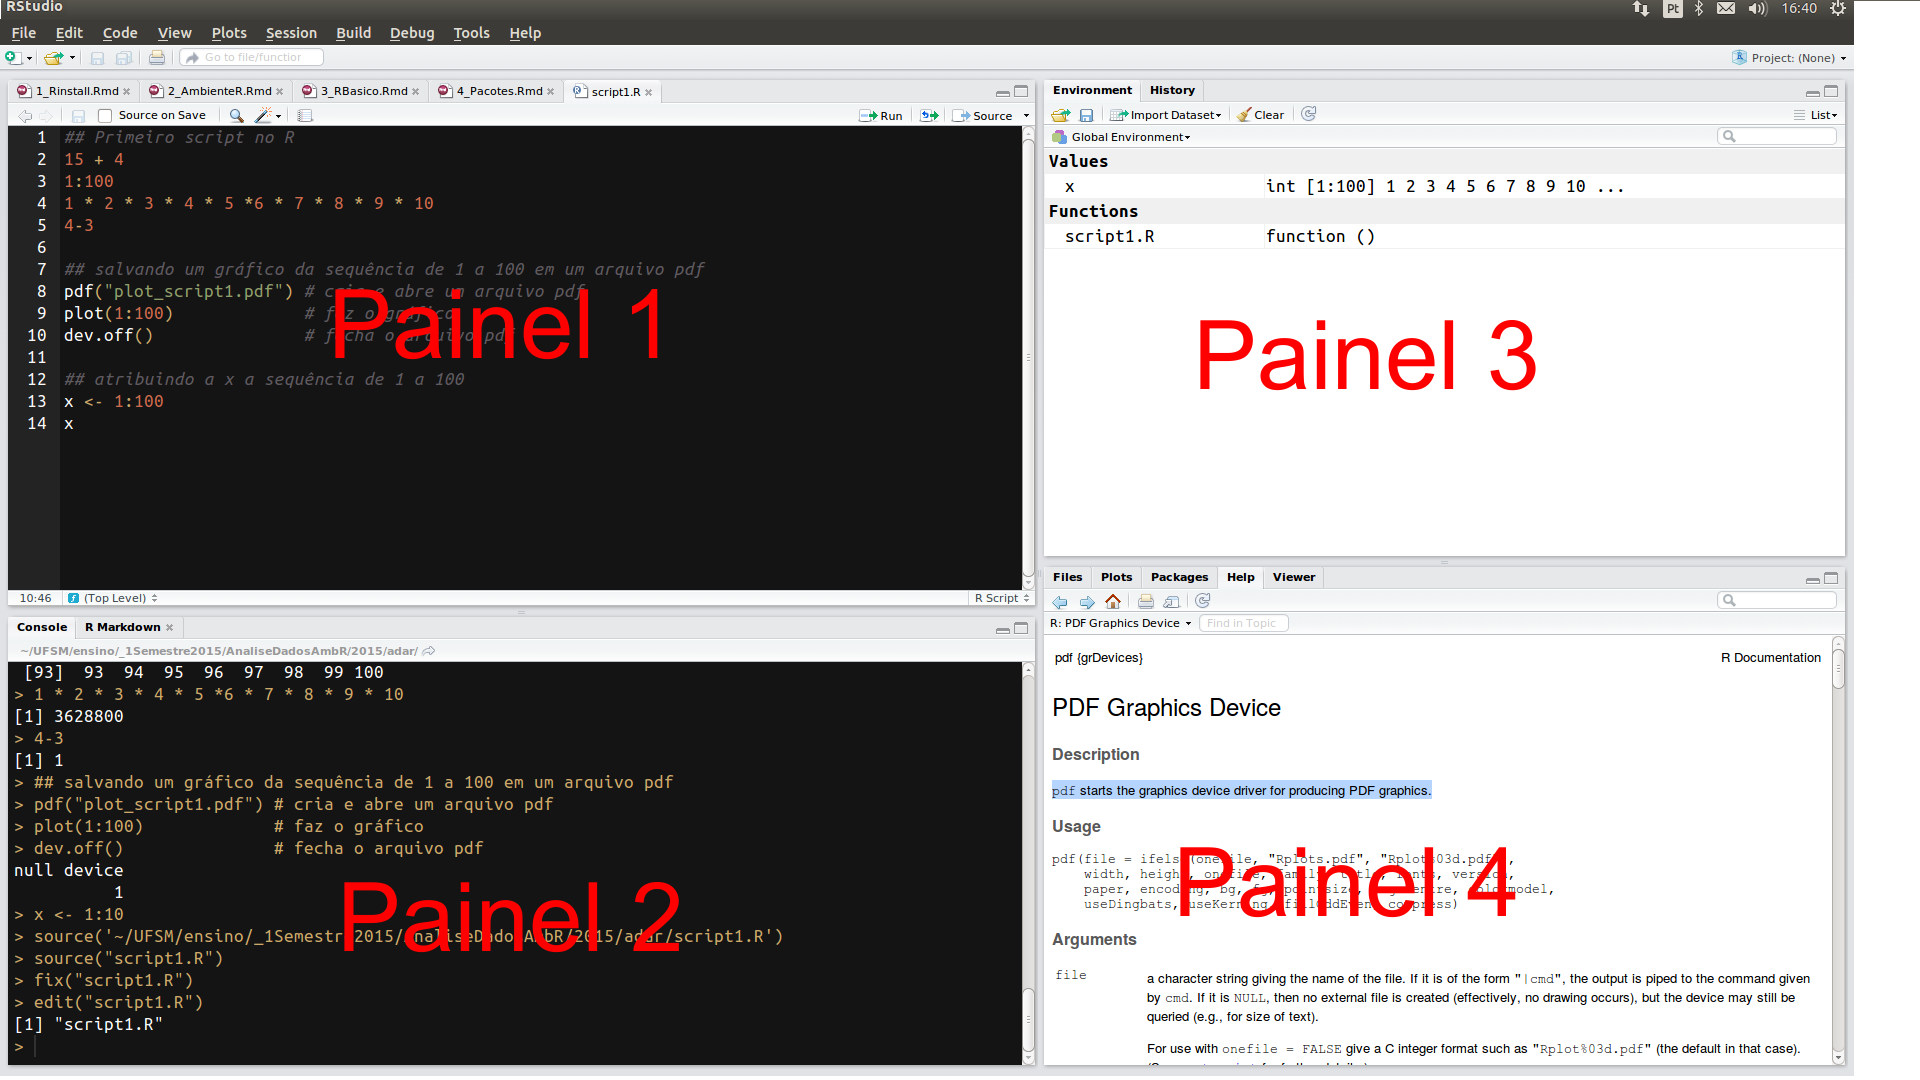
\includegraphics[width=26.67in]{images/Rstudio_panels} \caption{Rstudio}\label{fig:rstudio-fig}
\end{figure}

O RStudio possui 4 painéis principais:

\begin{enumerate}
\def\labelenumi{\arabic{enumi}.}
\item
  Editor para scripts e visualização de dados

  \begin{itemize}
  \tightlist
  \item
    abrir e criar scripts
  \item
    rodar scripts
  \item
    código com sintaxe realçada
  \item
    rodar partes do código \texttt{\textless{}Ctrl+enter\textgreater{}}
  \item
    rodar todo script \texttt{\textless{}Ctrl+Shift+S\textgreater{}}
  \item
    autopreenchimento das funções \texttt{\textless{}tab\textgreater{}}
  \item
    comentar linhas \texttt{\textless{}Ctrl+Shift+C\textgreater{}}
  \item
    desfazer \texttt{\textless{}Ctrl+Z\textgreater{}}
  \item
    refazer \texttt{\textless{}Ctrl+Shift+Z\textgreater{}}
  \item
    referência para teclas de atalho
    \texttt{\textless{}Alt+Shift+K\textgreater{}}
  \item
    abrir script com \texttt{\textless{}Ctrl+Click\textgreater{}}
  \item
    encontrar e substituir \texttt{Ctrl+F}
  \end{itemize}
\item
  Console do R
\item
  Navegador do espaço de trabalho e histórico de comandos
\item
  Arquivos/Plots/Pacotes/Ajuda/Visualizador
\end{enumerate}

Configuração de texto e painéis em:

\begin{itemize}
\tightlist
\item
  Menus

  \begin{itemize}
  \tightlist
  \item
    Tools \textgreater{} global Options \textgreater{} Appearance

    \begin{itemize}
    \tightlist
    \item
      mostrar linhas, alterar realce da sintaxe
    \end{itemize}
  \item
    Session
  \item
    Plots
  \end{itemize}
\end{itemize}

Para saber mais sobre os recursos fornecidos pelo RStudio assista ao
vídeo
\emph{\href{https://www.rstudio.com/resources/webinars/rstudio-essentials-webinar-series-part-1/}{RStudio
Essencials}}. Isso o ajudará a usar mais efetivamente o RStudio.

\textbf{Folha de referência do RStudio}

\begin{figure}

{\centering 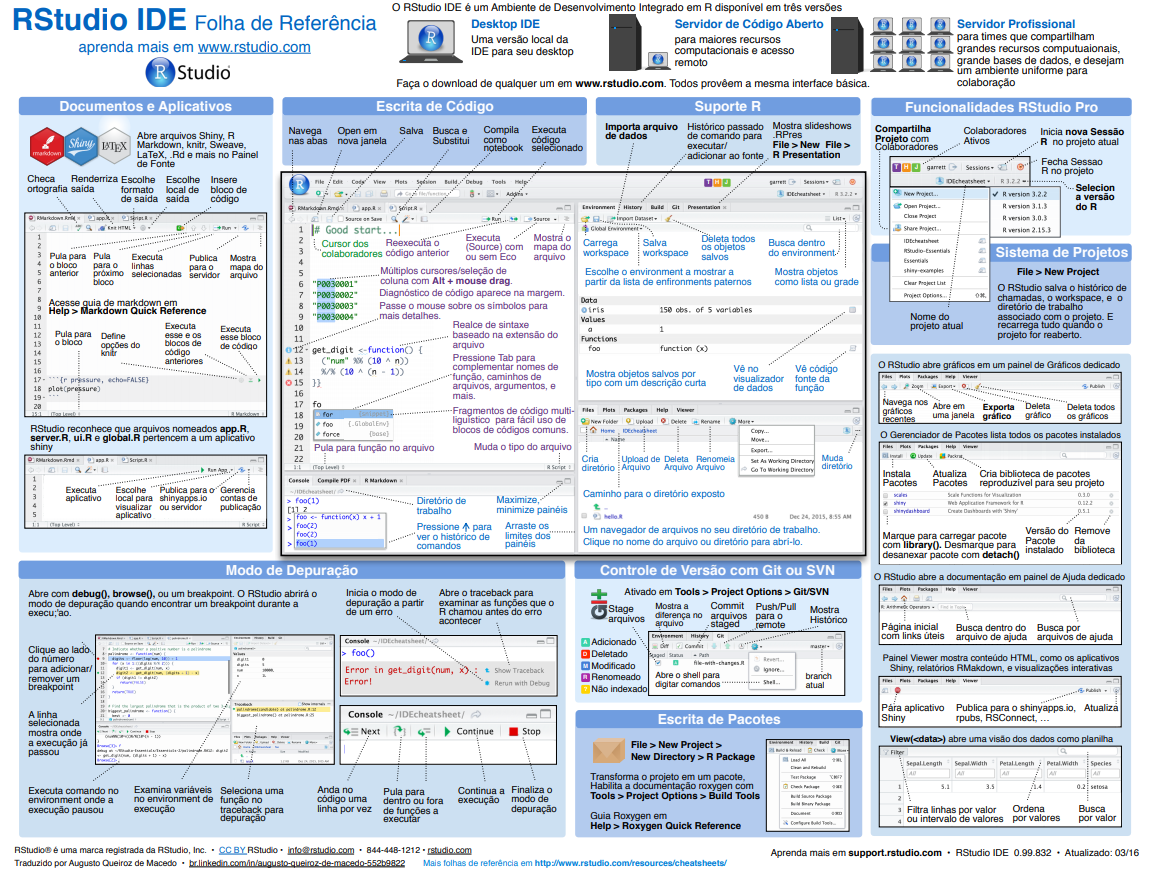
\includegraphics[width=1\linewidth]{images/print-screen-folha-ref-rstudio} 

}

\caption{Folha de referência do RStudio, disponível em https://www.rstudio.com/wp-content/uploads/2016/03/rstudio-IDE-cheatsheet-portuguese.pdf}\label{fig:cheat-sheet}
\end{figure}

\chapter{Operações básicas}\label{operbasic}

Nesta seção veremos:

\begin{itemize}
\tightlist
\item
  operações aritméticas básicas com 
\item
  a atribuição de valores a uma variável
\item
  o uso de funções matemáticas internas do 
\item
  valores numéricos especiais do 
\item
  os cuidados ao nomear variáveis
\end{itemize}

\section{Convenção}\label{convencao}

A partir deste capítulo, os códigos a serem avaliadas no terão o prompt
do (\texttt{\textgreater{}}) omitidos. Essa convenção é para tornar mais
fácil a ação de copiar e colar os códigos na linha de comando do . O
resultado da avaliação das expressões será mostrado precedido do símbolo
(\texttt{\#\textgreater{}}). Esses valores são os resultados que
esperam-se sejam reproduzidos pelo leitor na sessão do em seu
computador. Por exemplo:

\begin{Shaded}
\begin{Highlighting}[]
\DecValTok{1}\OperatorTok{:}\DecValTok{5}
\CommentTok{#> [1] 1 2 3 4 5}
\end{Highlighting}
\end{Shaded}

No trecho de código acima, a primeira linha contém o código a ser
copiado pelo leitor para execução em seu computador. A segunda linha é a
saída do código avaliado pelo R.

\section{Calculadora}\label{calculadora}

O é uma calculadora turbinada com diversas funções matemáticas
disponíveis. Para quem não conhece o , essa uma forma de familiarizar-se
com a linha de comandos.

\subsection{Aritmética básica}\label{aritmetica-basica}

Todas operações feitas em uma calculadora podem ser realizadas na linha
de comandos do .

\begin{Shaded}
\begin{Highlighting}[]
\DecValTok{10} \OperatorTok{+}\StringTok{ }\DecValTok{2} \OperatorTok{+}\StringTok{ }\DecValTok{4}
\CommentTok{#> [1] 16}
\CommentTok{# Exemplo de divisao }
\NormalTok{(}\DecValTok{5} \OperatorTok{+}\StringTok{ }\DecValTok{14}\NormalTok{)}\OperatorTok{/}\DecValTok{2}
\CommentTok{#> [1] 9.5}
\CommentTok{# exponenciação}
\DecValTok{2}\OperatorTok{^}\DecValTok{3}
\CommentTok{#> [1] 8}
\DecValTok{4}\OperatorTok{^}\FloatTok{0.5}
\CommentTok{#> [1] 2}
\CommentTok{# operador artimético para se determinar o resto de uma divisao}
\DecValTok{10} \OperatorTok\StringTok{ }\DecValTok{2}
\CommentTok{#> [1] 0}
\DecValTok{2001} \OperatorTok\StringTok{ }\DecValTok{2}
\CommentTok{#> [1] 1}
\CommentTok{# o inteiro do quociente }
\DecValTok{11} \OperatorTok\StringTok{ }\DecValTok{2}
\CommentTok{#> [1] 5}
\end{Highlighting}
\end{Shaded}

\begin{rmdwarning}
Note que no \texttt{r\ rblue}, o separador decimal é o ponto ".", ao
invés da vírgula "," usada na notação brasileira. As vírgulas tem a
finalidade de separar os argumentos nas chamadas de funções, tal como em
\texttt{log(x\ =\ 10,\ base\ =\ 10)}.
\end{rmdwarning}

Conheça mais operadores aritméticos, digitando na linha de comando:

\begin{Shaded}
\begin{Highlighting}[]
\NormalTok{?}\StringTok{"Arithmetic"}
\end{Highlighting}
\end{Shaded}

A janela que se abrirá mostrará o texto que faz parte do manual de ajuda
do .

\subsection{Constantes}\label{constantes}

O R possui algumas constantes pré-definidas, como o a constante pi
(\(\pi\)).

\begin{Shaded}
\begin{Highlighting}[]
\NormalTok{pi}
\CommentTok{#> [1] 3.141593}
\end{Highlighting}
\end{Shaded}

O também tem vetores de caracteres pré-definidos, são eles:

\begin{Shaded}
\begin{Highlighting}[]
\NormalTok{LETTERS}
\CommentTok{#>  [1] "A" "B" "C" "D" "E" "F" "G" "H" "I" "J" "K" "L" "M" "N" "O" "P" "Q"}
\CommentTok{#> [18] "R" "S" "T" "U" "V" "W" "X" "Y" "Z"}
\NormalTok{letters}
\CommentTok{#>  [1] "a" "b" "c" "d" "e" "f" "g" "h" "i" "j" "k" "l" "m" "n" "o" "p" "q"}
\CommentTok{#> [18] "r" "s" "t" "u" "v" "w" "x" "y" "z"}
\NormalTok{month.abb}
\CommentTok{#>  [1] "Jan" "Feb" "Mar" "Apr" "May" "Jun" "Jul" "Aug" "Sep" "Oct" "Nov"}
\CommentTok{#> [12] "Dec"}
\NormalTok{month.name}
\CommentTok{#>  [1] "January"   "February"  "March"     "April"     "May"      }
\CommentTok{#>  [6] "June"      "July"      "August"    "September" "October"  }
\CommentTok{#> [11] "November"  "December"}
\end{Highlighting}
\end{Shaded}

Note que caracteres estão sempre entre aspas: \texttt{""}.

``caracteres são entre aspas''

\begin{Shaded}
\begin{Highlighting}[]
\NormalTok{aeiou}
\CommentTok{#> Error in eval(expr, envir, enclos): object 'aeiou' not found}
\end{Highlighting}
\end{Shaded}

\begin{Shaded}
\begin{Highlighting}[]
\StringTok{"aeiou"}
\CommentTok{#> [1] "aeiou"}
\end{Highlighting}
\end{Shaded}

\subsection{Funções matemáticas
internas}\label{funcoes-matematicas-internas}

Existem diversas funções internas do que permitem, por exemplo, sortear
números aleatóriamente, arrendondar números, calcular o fatorial,
calcular o seno, cosseno de um ângulo e etc. A sintaxe para chamar uma
função no é:

\texttt{funcão(argumento)}

Por exemplo:

\begin{Shaded}
\begin{Highlighting}[]
\CommentTok{# funções trigonométricas}
\KeywordTok{sin}\NormalTok{(pi}\OperatorTok{/}\DecValTok{6}\NormalTok{)}
\CommentTok{#> [1] 0.5}
\KeywordTok{cos}\NormalTok{(pi)}
\CommentTok{#> [1] -1}
\CommentTok{# raiz quadrada}
\KeywordTok{sqrt}\NormalTok{(}\DecValTok{100}\NormalTok{)}
\CommentTok{#> [1] 10}
\CommentTok{# exponencial}
\KeywordTok{exp}\NormalTok{(}\DecValTok{1}\NormalTok{)}
\CommentTok{#> [1] 2.718282}
\CommentTok{# fatorial}
\KeywordTok{factorial}\NormalTok{(}\DecValTok{4}\NormalTok{)}
\CommentTok{#> [1] 24}
\end{Highlighting}
\end{Shaded}

No você verá que parênteses são frequentemente utilizados. Eles são
sempre associados à funções. Qualquer palavra antecedendo um parênteses
é uma função.

Para ver a lista completa de funções trigonométricas:

\begin{Shaded}
\begin{Highlighting}[]
\NormalTok{?}\StringTok{"Trig"}
\end{Highlighting}
\end{Shaded}

\subsection{Valores numéricos
especiais}\label{valores-numericos-especiais}

Um caso particular sobre operação aritméticas no , são os valores
numéricos \texttt{Inf}(Infinito) e \texttt{NaN} que resultam de
operações como as mostradas na Tabela \ref{tab:tab-num-esp}.
\texttt{NaN} é a abreviação para valor indefinido (do termo em inglês
\emph{Not a Number}). Geralmente surge quando um cálculo não tem sentido
matemático ou não pode ser propriamente realizado.

A demonstração das diferentes formas de se obter essas constantes
especiais é importante para entender a origem delas durante a execução
de um script mais extenso.

\begin{table}

\caption{\label{tab:tab-num-esp}Exemplos de operações que resultam em NaN ou $\pm\infty$ .}
\centering
\begin{tabular}[t]{c|c}
\hline
operação & resultado\\
\hline
2/0 & Inf\\
\hline
-12/0 & -Inf\\
\hline
log(0) & -Inf\\
\hline
(c(-3, 3))\textasciicircum{}Inf & NaN, Inf\\
\hline
0*Inf & NaN\\
\hline
log(-0.5) & NaN\\
\hline
sqrt(-1) & NaN\\
\hline
0/0 & NaN\\
\hline
Inf-Inf & NaN\\
\hline
mean(c(NA, NA), na.rm = TRUE) & NaN\\
\hline
\end{tabular}
\end{table}

Por outro lado abaixo mostra-se alguns exemplos operações válidas com
estes valores especiais.

\begin{Shaded}
\begin{Highlighting}[]
\KeywordTok{exp}\NormalTok{(}\OperatorTok{-}\OtherTok{Inf}\NormalTok{)}
\CommentTok{#> [1] 0}
\NormalTok{(}\DecValTok{0}\OperatorTok{:}\DecValTok{1}\NormalTok{)}\OperatorTok{^}\OtherTok{Inf}
\CommentTok{#> [1] 0 1}
\DecValTok{0}\OperatorTok{/}\OtherTok{Inf}
\CommentTok{#> [1] 0}
\NormalTok{(}\KeywordTok{c}\NormalTok{(}\OperatorTok{-}\DecValTok{1}\NormalTok{, }\DecValTok{1}\NormalTok{)}\OperatorTok{*}\OtherTok{Inf}\NormalTok{)}\OperatorTok{^}\DecValTok{0}
\CommentTok{#> [1] 1 1}
\DecValTok{0}\OperatorTok{^}\DecValTok{0}
\CommentTok{#> [1] 1}
\end{Highlighting}
\end{Shaded}

Outra constante especial do é o \texttt{NA} (\emph{Not Available}) que
representa valor faltante, um problema comum em análise de dados.
Qualquer operação envolvendo \texttt{NA} resultará em \texttt{NA}
(Tabela \ref{tab:tab-nas}).

\begin{table}

\caption{\label{tab:tab-nas}Operações com NA.}
\centering
\begin{tabular}[t]{c|c}
\hline
operação & resultado\\
\hline
NA + 5 & NA\\
\hline
sqrt(NA) & NA\\
\hline
NA\textasciicircum{}2 & NA\\
\hline
NA/NaN & NA\\
\hline
\end{tabular}
\end{table}

\subsection{Notação científica e número de
dígitos}\label{notacao-cientifica-e-numero-de-digitos}

Na maioria das vezes precisamos trabalhar com números grandes e
consequentemente acabamos usando uma notação científica ou exponencial.
No há diferentes formas de representar números com expoentes:

\begin{Shaded}
\begin{Highlighting}[]
\FloatTok{1.2e-6}
\CommentTok{#> [1] 1.2e-06}
\CommentTok{# expressões equivalentes}
\FloatTok{1.2E6}\NormalTok{; }\FloatTok{1.2}\OperatorTok{*}\DecValTok{10}\OperatorTok{^}\DecValTok{6}  
\CommentTok{#> [1] 1200000}
\CommentTok{#> [1] 1200000}
\end{Highlighting}
\end{Shaded}

Os resultados dos cálculos no são mostrados com 7 dígitos
significativos, o que pode ser verificado pela \texttt{getOptions()}. É
possível mudar para \texttt{n} dígitos usando a função
\texttt{options()}, conforme exemplo abaixo.

\begin{Shaded}
\begin{Highlighting}[]
\CommentTok{# opção de dígitos padrão}
\KeywordTok{getOption}\NormalTok{(}\StringTok{"digits"}\NormalTok{)}
\CommentTok{#> [1] 7}
\KeywordTok{exp}\NormalTok{(}\DecValTok{1}\NormalTok{)}
\CommentTok{#> [1] 2.718282}
\CommentTok{# alterando para 14}
\KeywordTok{options}\NormalTok{(}\DataTypeTok{digits =} \DecValTok{14}\NormalTok{)}
\KeywordTok{exp}\NormalTok{(}\DecValTok{1}\NormalTok{)}
\CommentTok{#> [1] 2.718281828459}
\KeywordTok{getOption}\NormalTok{(}\StringTok{"digits"}\NormalTok{)}
\CommentTok{#> [1] 14}
\CommentTok{# redefinindo para o número de casas decimais padrão}
\KeywordTok{options}\NormalTok{(}\DataTypeTok{digits =} \DecValTok{7}\NormalTok{)}
\KeywordTok{getOption}\NormalTok{(}\StringTok{"digits"}\NormalTok{)}
\CommentTok{#> [1] 7}
\end{Highlighting}
\end{Shaded}

\section{Variáveis}\label{variaveis}

\subsection{Formas de atribuição}\label{formas-de-atribuicao}

\subsubsection{Variável recebe valor}\label{variavel-recebe-valor}

Até agora nós usamos expressões para fazer uma operação e obter um
resultado. O termo "expressão" significa uma sentença de código que pode
ser executada. Se a avaliação de uma expressão é salva usando o operador
\texttt{\textless{}-}, esta combinação é chamada "atribuição". O
resultado da "atribuição" é armazenado em uma variável e pode ser
utilizado posteriormente. Então uma variável é um nome usado para
guardar os dados.

\texttt{variavel\ \textless{}-\ valor}

\begin{Shaded}
\begin{Highlighting}[]
\NormalTok{p <-}\StringTok{ }\DecValTok{1013}
\CommentTok{# para mostrar a variável digite o nome da variável}
\NormalTok{p}
\CommentTok{#> [1] 1013}
\CommentTok{# ou use a função print()}
\KeywordTok{print}\NormalTok{(p)}
\CommentTok{#> [1] 1013}
\end{Highlighting}
\end{Shaded}

O R diferencia letras maiúsculas de minúsculas. Portanto \texttt{p} e
\texttt{P} são variáveis diferentes.

\begin{Shaded}
\begin{Highlighting}[]
\NormalTok{p}
\CommentTok{#> [1] 1013}
\NormalTok{P}
\CommentTok{#> Error in eval(expr, envir, enclos): object 'P' not found}
\end{Highlighting}
\end{Shaded}

Como criamos apenas a variável \texttt{p}, \texttt{P} não foi
encontrada.

A variável \texttt{p} pode ser utilizado para criar outras variáveis.

\begin{Shaded}
\begin{Highlighting}[]
\NormalTok{p_pa <-}\StringTok{ }\NormalTok{p }\OperatorTok{*}\StringTok{ }\DecValTok{100}
\CommentTok{# pressão em Pascal}
\NormalTok{p_pa}
\CommentTok{#> [1] 101300}
\end{Highlighting}
\end{Shaded}

A seta de atribuição pode ser usada em qualquer sentido. Parênteses,
além de estarem sempre acompanhando uma função, também são usados para
indicar a prioridade dos cálculos.

\begin{Shaded}
\begin{Highlighting}[]
\DecValTok{7}\OperatorTok{/}\DecValTok{3} \OperatorTok{+}\StringTok{ }\FloatTok{0.6}\NormalTok{ ->}\StringTok{ }\NormalTok{y1}
\NormalTok{ y1}
\CommentTok{#> [1] 2.933333}
\DecValTok{7}\OperatorTok{/}\NormalTok{(}\DecValTok{3} \OperatorTok{+}\StringTok{ }\FloatTok{0.6}\NormalTok{) ->}\StringTok{ }\NormalTok{y2}
\NormalTok{ y2}
\CommentTok{#> [1] 1.944444}
\end{Highlighting}
\end{Shaded}

Os espaços em torno do símbolo de atribuição (\texttt{\textless{}-}) não
são obrigatórios mas eles ajudam na legibilidade do código.

\begin{Shaded}
\begin{Highlighting}[]
\NormalTok{x <-}\StringTok{ }\DecValTok{1}
\NormalTok{x }\OperatorTok{<}\StringTok{ }\OperatorTok{-}\DecValTok{1}
\CommentTok{# atribuição ou menor que?}
\NormalTok{x<-}\DecValTok{1} 
\end{Highlighting}
\end{Shaded}

Vamos criar uma variável chamada \texttt{ndias3} que recebe o nº de dias
no mês de Março e \texttt{ndias4} que recebe o nº de dias no mês de
Abril.

\begin{Shaded}
\begin{Highlighting}[]
\NormalTok{nd3 <-}\StringTok{ }\DecValTok{31}
\NormalTok{nd4 <-}\StringTok{ }\DecValTok{30}
\end{Highlighting}
\end{Shaded}

O total de dias nos meses de março e abril será armazenado na variável
\texttt{totdias}:

\begin{Shaded}
\begin{Highlighting}[]
\NormalTok{totd <-}\StringTok{ }\NormalTok{nd3 }\OperatorTok{+}\StringTok{ }\NormalTok{nd4}
\NormalTok{totd}
\CommentTok{#> [1] 61}
\end{Highlighting}
\end{Shaded}

A atribuição de um mesmo valor para diferentes variáveis pode ser feita
da seguinte forma:

\begin{Shaded}
\begin{Highlighting}[]
\CommentTok{# número de dias em cada mês}
\NormalTok{jan <-}\StringTok{ }\NormalTok{mar <-}\StringTok{ }\NormalTok{mai <-}\StringTok{ }\NormalTok{jul <-}\StringTok{ }\NormalTok{ago <-}\StringTok{ }\NormalTok{out <-}\StringTok{ }\NormalTok{dez <-}\StringTok{ }\DecValTok{31}
\NormalTok{abr <-}\StringTok{ }\NormalTok{jun <-}\StringTok{ }\NormalTok{set <-}\StringTok{ }\NormalTok{nov <-}\StringTok{ }\DecValTok{30}
\NormalTok{fev <-}\StringTok{ }\DecValTok{28}
\CommentTok{# verificação}
\NormalTok{jan}
\CommentTok{#> [1] 31}
\NormalTok{jul}
\CommentTok{#> [1] 31}
\NormalTok{jun}
\CommentTok{#> [1] 30}
\NormalTok{set}
\CommentTok{#> [1] 30}
\NormalTok{fev}
\CommentTok{#> [1] 28}
\end{Highlighting}
\end{Shaded}

Nós estamos definindo a variável, digitando o nome dela na linha de
comando e teclando enter para ver o resultado. Há uma forma mais prática
de fazer isso e mostrar o resultado cercando a atribuição por
parênteses:

\begin{Shaded}
\begin{Highlighting}[]
\CommentTok{# ao invés de }
\CommentTok{# tar <- 20}
\CommentTok{# tar}
\CommentTok{# é mais prático}
\NormalTok{(tar <-}\StringTok{ }\DecValTok{20}\NormalTok{) }
\CommentTok{#> [1] 20}
\end{Highlighting}
\end{Shaded}

Se desejamos calcular e já visualizar o valor da pressão de vapor de
saturação obtida com a
\href{https://en.wikipedia.org/wiki/Tetens_equation}{equação de Tetens},
podemos fazer:

\begin{Shaded}
\begin{Highlighting}[]
\NormalTok{(es <-}\StringTok{ }\FloatTok{0.611} \OperatorTok{*}\StringTok{ }\KeywordTok{exp}\NormalTok{((}\FloatTok{17.269} \OperatorTok{*}\StringTok{ }\NormalTok{tar)}\OperatorTok{/}\NormalTok{(tar }\OperatorTok{+}\StringTok{ }\FloatTok{237.3}\NormalTok{)))}
\CommentTok{#> [1] 2.338865}
\end{Highlighting}
\end{Shaded}

Quando usamos a mesma variável numa sequência de atribuições o seu valor
é sobrescrito. Portanto não é bom usar nomes que já foram usados antes,
exceto se a intenção for realmente essa. Para saber os nomes das
variáveis já usados use a função \texttt{ls()}\footnote{Essa lista de
  variáveis também é mostrada no painel \emph{Environment} do RStudio
  (canto direito superior, aba \emph{Environment}).} para verificar as
variáveis existentes:

\begin{Shaded}
\begin{Highlighting}[]
\KeywordTok{ls}\NormalTok{()}
\CommentTok{#>  [1] "abr"        "ago"        "dez"        "es"         "esp_num_df"}
\CommentTok{#>  [6] "fev"        "jan"        "jul"        "jun"        "mai"       }
\CommentTok{#> [11] "mar"        "nd3"        "nd4"        "nov"        "oper"      }
\CommentTok{#> [16] "oper_nas"   "out"        "p"          "pcks"       "p_pa"      }
\CommentTok{#> [21] "rblue"      "res"        "set"        "tar"        "totd"      }
\CommentTok{#> [26] "y1"         "y2"}
\end{Highlighting}
\end{Shaded}

\begin{Shaded}
\begin{Highlighting}[]
\NormalTok{totd <-}\StringTok{ }\NormalTok{jan}\OperatorTok{*}\DecValTok{7}\NormalTok{; totd <-}\StringTok{ }\NormalTok{totd }\OperatorTok{+}\StringTok{ }\NormalTok{fev; totd <-}\StringTok{ }\NormalTok{totd }\OperatorTok{+}\StringTok{ }\DecValTok{4}\OperatorTok{*}\NormalTok{abr}
\NormalTok{totd}
\CommentTok{#> [1] 365}
\end{Highlighting}
\end{Shaded}

\subsubsection{\texorpdfstring{Atribuição com a função
\texttt{assign()}}{Atribuição com a função assign()}}\label{atribuicao-com-a-funcao-assign}

Outra forma de atribuição é através da função \texttt{assign()}:

\begin{Shaded}
\begin{Highlighting}[]
\NormalTok{es}
\CommentTok{#> [1] 2.338865}
\KeywordTok{assign}\NormalTok{(}\DataTypeTok{x =} \StringTok{"es_hpa"}\NormalTok{, }\DataTypeTok{value =}\NormalTok{ es}\OperatorTok{/}\DecValTok{10}\NormalTok{)}
\NormalTok{es_hpa}
\CommentTok{#> [1] 0.2338865}
\CommentTok{# usando função assign sem nome dos parâmetros}
\KeywordTok{assign}\NormalTok{(}\StringTok{"u"}\NormalTok{, }\FloatTok{2.5}\NormalTok{)}
\NormalTok{u}
\CommentTok{#> [1] 2.5}
\end{Highlighting}
\end{Shaded}

Um exemplo mais elaborado de uso da função \texttt{assign()} para criar
várias variáveis pode ser visto
\href{https://gist.github.com/lhmet/d28856ed16690bb45d5be36ea4f5d458\#file-assign-ex-rmd}{aqui}.

\subsection{Removendo variáveis}\label{removendo-variaveis}

Para remover variáveis usa-se a função \texttt{rm()}.

\begin{Shaded}
\begin{Highlighting}[]
\CommentTok{# lista de variáveis existentes}
\KeywordTok{ls}\NormalTok{()}
\CommentTok{#>  [1] "abr"        "ago"        "dez"        "es"         "es_hpa"    }
\CommentTok{#>  [6] "esp_num_df" "fev"        "jan"        "jul"        "jun"       }
\CommentTok{#> [11] "mai"        "mar"        "nd3"        "nd4"        "nov"       }
\CommentTok{#> [16] "oper"       "oper_nas"   "out"        "p"          "pcks"      }
\CommentTok{#> [21] "p_pa"       "rblue"      "res"        "set"        "tar"       }
\CommentTok{#> [26] "totd"       "u"          "y1"         "y2"}
\end{Highlighting}
\end{Shaded}

Vamos remover a variável \texttt{u} criada previamente e ver a lista de
objetos no espaço de trabalho.

\begin{Shaded}
\begin{Highlighting}[]
\KeywordTok{rm}\NormalTok{(u)}
\CommentTok{# lista de variáveis existentes, sem u}
\KeywordTok{ls}\NormalTok{()}
\CommentTok{#>  [1] "abr"        "ago"        "dez"        "es"         "es_hpa"    }
\CommentTok{#>  [6] "esp_num_df" "fev"        "jan"        "jul"        "jun"       }
\CommentTok{#> [11] "mai"        "mar"        "nd3"        "nd4"        "nov"       }
\CommentTok{#> [16] "oper"       "oper_nas"   "out"        "p"          "pcks"      }
\CommentTok{#> [21] "p_pa"       "rblue"      "res"        "set"        "tar"       }
\CommentTok{#> [26] "totd"       "y1"         "y2"}
\end{Highlighting}
\end{Shaded}

Podemos remover mais de uma variável ao mesmo tempo.

\begin{Shaded}
\begin{Highlighting}[]
\KeywordTok{rm}\NormalTok{(es_hpa, es, tar, y1, y2)}
\CommentTok{# lista de variáveis existentes, sem es_hpa, es, tar, y1, y2}
\KeywordTok{ls}\NormalTok{()}
\CommentTok{#>  [1] "abr"        "ago"        "dez"        "esp_num_df" "fev"       }
\CommentTok{#>  [6] "jan"        "jul"        "jun"        "mai"        "mar"       }
\CommentTok{#> [11] "nd3"        "nd4"        "nov"        "oper"       "oper_nas"  }
\CommentTok{#> [16] "out"        "p"          "pcks"       "p_pa"       "rblue"     }
\CommentTok{#> [21] "res"        "set"        "totd"}
\end{Highlighting}
\end{Shaded}

Para remover todas variáveis do espaço de trabalho (use com cautela):

\begin{Shaded}
\begin{Highlighting}[]
\CommentTok{# apagando tudo}
\KeywordTok{rm}\NormalTok{(}\DataTypeTok{list =} \KeywordTok{ls}\NormalTok{())}
\KeywordTok{ls}\NormalTok{()}
\CommentTok{#> character(0)}
\end{Highlighting}
\end{Shaded}

\subsection{Nomeando variáveis}\label{nomeando-variaveis}

É preciso ter cuidado ao nomear variáveis no R porque existem algumas
regras:

\begin{itemize}
\tightlist
\item
  não iniciar com um número e não conter espaços
\end{itemize}

\begin{Shaded}
\begin{Highlighting}[]
\NormalTok{1oAno <-}\StringTok{ }\DecValTok{1990}
\NormalTok{raizDe10 <-}\StringTok{ }\KeywordTok{srt}\NormalTok{(}\DecValTok{2}\NormalTok{)}
\NormalTok{variavel teste <-}\StringTok{ }\DecValTok{67}
\end{Highlighting}
\end{Shaded}

\begin{Shaded}
\begin{Highlighting}[]
\CommentTok{# nomes alternativos para as variaveis}
\NormalTok{ano1 <-}\StringTok{ }\DecValTok{1990}
\NormalTok{variavel_teste <-}\StringTok{ }\DecValTok{67}
\NormalTok{variavel.teste <-}\StringTok{ }\DecValTok{68}
\end{Highlighting}
\end{Shaded}

\begin{itemize}
\item
  não conter símbolos especiais:

\begin{verbatim}
^, !, $, @, +, -, /, ou *
\end{verbatim}
\end{itemize}

\begin{Shaded}
\begin{Highlighting}[]
\NormalTok{dia}\OperatorTok{-}\DecValTok{1}\NormalTok{ <-}\StringTok{ }\DecValTok{2}
\CommentTok{#> Error in dia - 1 <- 2: object 'dia' not found}
\CommentTok{# alternativa}
\NormalTok{dia_}\DecValTok{1}\NormalTok{ <-}\StringTok{ }\DecValTok{2}
\end{Highlighting}
\end{Shaded}

\begin{itemize}
\item
  evitar o uso de nomes usados em objetos do sistema (funções internas
  do R ou constantes como o número \(\pi\)):

\begin{verbatim}
c q  s  t  C  D  F  I  T  diff  exp  log  mean  pi  range  rank  var

FALSE  Inf  NA  NaN  NULL TRUE 

break  else  for  function  if  in  next  repeat  while
\end{verbatim}
\item
  variáveis com acento são permitidas mas não recomendadas.
\end{itemize}

\begin{Shaded}
\begin{Highlighting}[]
\NormalTok{verão <-}\StringTok{ "DJF"}
\NormalTok{verão}
\CommentTok{#> [1] "DJF"}
\end{Highlighting}
\end{Shaded}

\begin{rmdtip}
Há limitações de interpretação do R para caracteres latinos como cedilha
e acentos. Por isso não recomenda-se o uso destes caracteres para nomear
variáveis.
\end{rmdtip}

Uma boa prática de programação é dar nomes informativos às variáveis
para maior legibilidade do código. Uma boa referência para isso é a
seção \href{http://style.tidyverse.org/syntax.html}{\textbf{Sintaxe}} do
\href{http://style.tidyverse.org/}{Guia de estilo tidyverse (ou universo
arrumado)}.

Apesar do ganho de legibilidade do código com a aplicação das regras de
formatação de código do \emph{tidyverse} é difícil de lembrar de todas
elas.

Mas este não é mais um problema, pois o pacote
\href{http://styler.r-lib.org/}{styler} fornece funções para estilizar o
seu código padrão \emph{tidyverse}.

\begin{Shaded}
\begin{Highlighting}[]
\KeywordTok{install.packages}\NormalTok{(}\StringTok{"styler"}\NormalTok{)}
\KeywordTok{library}\NormalTok{(styler)}
\end{Highlighting}
\end{Shaded}

As funções são acessíveis Através do menu \emph{Addins} do RStudio e
incluem as opções de: estilizar um arquivo e uma região destacada do
código.

\includegraphics{images/styler_0.1.gif}

\section{Exercícios}\label{exercicios}

\begin{enumerate}
\def\labelenumi{\arabic{enumi}.}
\tightlist
\item
  Execute as seguintes expressões no R mostrando os resultados obtidos.
\end{enumerate}

\begin{Shaded}
\begin{Highlighting}[]
\DecValTok{1} \OperatorTok{+}\StringTok{ }\DecValTok{1}
\DecValTok{100}\OperatorTok{:}\DecValTok{130}
\DecValTok{5} \OperatorTok{-}\StringTok{ }\OperatorTok{+}\DecValTok{1}
\DecValTok{3}\NormalTok{ % }\DecValTok{5}
\DecValTok{2} \OperatorTok{*}\StringTok{ }\DecValTok{3}
\DecValTok{4} \OperatorTok{-}\StringTok{ }\DecValTok{1}
\DecValTok{6} \OperatorTok{/}\StringTok{ }\NormalTok{(}\DecValTok{4} \OperatorTok{-}\StringTok{ }\DecValTok{1}\NormalTok{)}
\end{Highlighting}
\end{Shaded}

\begin{center}\rule{0.5\linewidth}{\linethickness}\end{center}

\begin{enumerate}
\def\labelenumi{\arabic{enumi}.}
\setcounter{enumi}{1}
\tightlist
\item
  Utilize uma expressão para cada item.

  \begin{enumerate}
  \def\labelenumii{\alph{enumii}.}
  \tightlist
  \item
    Escolha um número e some 3 a ele.
  \item
    Multiplique o resultado por 2.
  \item
    Subtraia 10 da resposta.
  \item
    Divida o que foi obtido por 4.
  \end{enumerate}
\end{enumerate}

\begin{center}\rule{0.5\linewidth}{\linethickness}\end{center}

\begin{enumerate}
\def\labelenumi{\arabic{enumi}.}
\setcounter{enumi}{2}
\tightlist
\item
  Calcule \(\sqrt{16}\), \({16^{0.5}}^{3}\), \({(16^{0.5})}^{3}\) e
  \(4^{\frac{3}{2}}\).
\end{enumerate}

\begin{center}\rule{0.5\linewidth}{\linethickness}\end{center}

\begin{enumerate}
\def\labelenumi{\arabic{enumi}.}
\setcounter{enumi}{3}
\tightlist
\item
  Teste as expressões \texttt{log10(1000)}, \texttt{log(1000)},
  \texttt{exp(log(1000))}. Depois teste a expressão \texttt{log2(64)}.
  Verifique se você entendeu as diferentes funções logarítmicas.
\end{enumerate}

\begin{center}\rule{0.5\linewidth}{\linethickness}\end{center}

\begin{enumerate}
\def\labelenumi{\arabic{enumi}.}
\setcounter{enumi}{4}
\item
  Defina as variáveis abaixo tomando cuidados ao nomear as variáveis,
  conforme visto em sala de aula. Mostre os valores para as seguintes
  constantes:

  \begin{enumerate}
  \def\labelenumii{\alph{enumii}.}
  \item
    Velocidade da luz:
    \(\nu = 2.998 \times 10^{8} \left[m \, s^{-1}\right]\)
  \item
    Carga elementar ou eletrônica:
    \(e = 1.602 \times 10^{-19} \left[C\right]\)
  \item
    Permissividade do vácuo:
    \(\epsilon_{0} = 8.85 \times 10^{-12} \left[C^{2} \, N^{-1} \, m^{2}\right]\)
  \item
    Constante de Planck: \(h=6.626 \times 10^{-34} \left[J \, s\right]\)
  \item
    Constante de Stefan Boltzman:
    \(\sigma = 5.67 \times 10^{-8} \left[W \, m^{-2} \, K^{-4}\right]\)\\
  \item
    Constante solar: \(S_{0} = 1380 \left[W \, m^{-2}\right]\)
  \item
    Constante de Avogadro:
    \(N_{A} = 6.022 \times 10^{23} \left[mol^{-1}\right]\)
  \item
    Constante dos gases para o ar seco:
    \(R_{d} = 287.04 \left[J \, K^{-1} \, kg^{-1}\right]\)
  \item
    Constante dos gases ideais para o vapor:
    \(R_{w} = 461.5 \left[J \, K^{-1} \, kg^{-1}\right]\)
  \item
    Densidade do ar seco para CNTP (à 0 ° C em 1000 mb):
    \(\rho=1.2754 \left[kg \, m^{-3}\right]\)
  \item
    Pressão média ao nível médio do mar para atmosfera padrão:
    \(P_{0}=1013.25 \left[mb\right]\)
  \item
    Temperatura ao nível médio do mar para atmosfera padrão:
    \(T_{0}=288.15 \left[K\right]\)
  \item
    Calor latente de vaporização ou condensação (à 0 °C):
    \(\lambda_{v} = 2.501 \times 10^{6}\left[J \, kg^{-1}\right]\)
  \item
    Calor latente de fusão (à 0 °C):
    \(\lambda_{f} = 0.334 \times 10^{6}\left[J \, kg^{-1}\right]\)
  \item
    Massa molecular da água: \(M_w = 18.016 \left[g \, mol^{-1}\right]\)
  \item
    Peso molecular do ar: \(M_{ar} = 28.96 \left[g \, mol^{-1}\right]\)
  \item
    Raio da terra: \(r = 6.37 \times 10^{6} \left[m\right]\)
  \item
    Velocidade angular da Terra:
    \(\Omega=7.29 \times 10^{-5} \left[rad \, s^{-1}\right]\)
  \end{enumerate}
\end{enumerate}

\begin{center}\rule{0.5\linewidth}{\linethickness}\end{center}

\begin{enumerate}
\def\labelenumi{\arabic{enumi}.}
\setcounter{enumi}{5}
\item
  \begin{enumerate}
  \def\labelenumii{(\alph{enumii})}
  \tightlist
  \item
    Como você pode fazer para que a constante \texttt{pi} seja mostrada
    com 20 dígitos? (b) Como voltar a trabalhar a com 7 dígitos
    novamente? c. Mostre o número neperiano com 7 dígitos.
  \end{enumerate}
\end{enumerate}

\begin{center}\rule{0.5\linewidth}{\linethickness}\end{center}

\begin{enumerate}
\def\labelenumi{\arabic{enumi}.}
\setcounter{enumi}{6}
\tightlist
\item
  Determine a temperatura de búlbo úmido (\(T_{w}\)) usando a expressão
  empírica
  (\href{http://journals.ametsoc.org/doi/abs/10.1175/JAMC-D-11-0143.1\%5D}{Stull,
  2011}) abaixo. Salve os resultados em variáveis diferentes. Para uma
  temperatura do ar (\(T\)) de 20°C e Umidade relativa (\(UR\)) de 70\%,
  qual o valor de \texttt{Tw}? Defina variáveis para os valores \(T\) e
  (\(UR\)) e use-as na equação de \(T_{w}\).
\end{enumerate}

\[
\begin{aligned} 
T_{w}=T\cdot atan\left [ 0.151977\cdot \left ( UR+8.313659 \right )^{1/2} \right ]+ \\
atan\left (T+UR \right )-\\
atan\left ( UR-1.676331 \right )+\\
0.00391838\left ( UR \right )^{3/2}\cdot atan\left ( 0.023101\cdot UR \right )-\\
4.686035
\end{aligned} 
\]

\begin{center}\rule{0.5\linewidth}{\linethickness}\end{center}

\begin{enumerate}
\def\labelenumi{\arabic{enumi}.}
\setcounter{enumi}{7}
\tightlist
\item
  Determine os valores de umidade do solo:
\end{enumerate}

\begin{itemize}
\item
  no potencial hídrico de 10kPa (\(\theta_{10kPa}\))
\item
  na capacidade de campo (\(\theta_{33kPa}\))
\item
  no ponto de murcha permanente (\(\theta_{1500kPa}\))

  utilizando o conjunto de equações de pedotransferência abaixo
  (\href{https://dl.sciencesocieties.org/publications/sssaj/abstracts/67/4/1085}{Tomasela
  et al. 2003}):
\end{itemize}

\begin{center}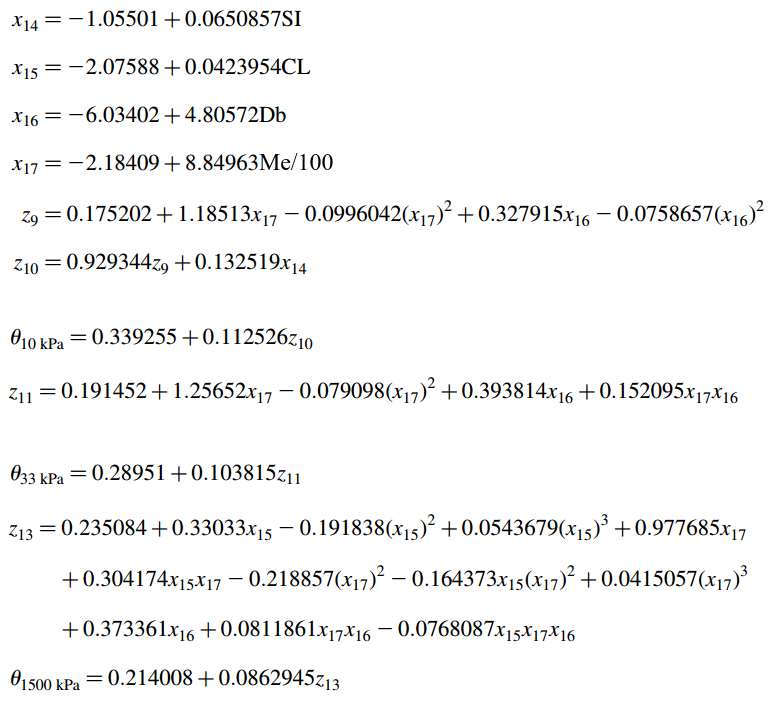
\includegraphics[width=0.88\linewidth]{images/conj-eqs-tomasella2003} \end{center}

\begin{itemize}
\tightlist
\item
  Considere \(SI = 16.29\) (\%), \(CL = 49.25\) (\%), \(Db = 1.25\)
  (\(g \, cm^{-3}\)), \(Me = 25\) (\%), onde \(SI\) é a porcentagem de
  silte no solo, \(CL\) é a porcentagem de argila, \(Db\) é a densidade
  do solo e \(Me\) é a umidade equivalente em \%.
\end{itemize}

\begin{center}\rule{0.5\linewidth}{\linethickness}\end{center}

\begin{enumerate}
\def\labelenumi{\arabic{enumi}.}
\setcounter{enumi}{8}
\tightlist
\item
  Arredonde para 2 casas decimais os resultados da questão 8. Dica ver
  \texttt{?round}.
\end{enumerate}

\begin{center}\rule{0.5\linewidth}{\linethickness}\end{center}

\begin{enumerate}
\def\labelenumi{\arabic{enumi}.}
\setcounter{enumi}{9}
\tightlist
\item
  Instale a \textbf{última versão do R} no (seu) computador usado para
  resolução desta lista. Crie um \emph{script} chamado
  \texttt{solucao-q10-NomeDoAluno.R} contendo os códigos gerados para
  solução das questões 7 e 8. Faça as seguintes alterações no código do
  \emph{script}:
\end{enumerate}

\begin{itemize}
\item
  no código da questão 8, utilize a temperatura do ar (\(T\)) de 30°C e
  Umidade relativa (\(UR\)) de 30\% para calcular \(Tw\).
\item
  no código da questão 9, considere \(SI = 13\) (\%), \(CL = 37\) (\%),
  \(Db = 1.3\) (\(g \, cm^{-3}\)), \(Me = 21\) (\%) para recalcular
  \(\theta_{10kPa}\), \(\theta_{33kPa}\) e \(\theta_{1500kPa}\).
\item
  após os códigos usados para resolver as questões 8 e 9, adicione uma
  nova linha com a expressão \texttt{sessionInfo()}.
\item
  Finalmente rode o \emph{script} usando o R no modo não iterativo.
  Anexe o arquivo de saída \texttt{solucao-q10-NomeDoAluno.Rout} como
  resposta para este problema.
\end{itemize}

\begin{center}\rule{0.5\linewidth}{\linethickness}\end{center}

\begin{rmdimportant}
\textbf{Instruções para entrega da resolução da lista de exercícios.}

A resolução da lista deve conter um único arquivo compactado nomeado
segundo o padrão \texttt{lista1-adar-NomedoAluno.zip}.

O arquivo compactado deve incluir pelo menos 3 arquivos:

\begin{enumerate}
\def\labelenumi{\arabic{enumi}.}
\item
  \texttt{solucao-q10-NomeDoAluno.R}: um \emph{script} com os códigos
  usados para resolver a questão 10.
\item
  \texttt{solucao-q10-NomeDoAluno.Rout} um arquivo texto de saída gerado
  (automaticamente) pelo R quando usado no modo não iterativo
  (\emph{Batch}). Também faz parte da resolução da questão 10.
\item
  \texttt{lista1-adar-NomedoAluno.Rmd}: arquivo \textbf{Rmarkdown}
  gerado no RStudio
  (\texttt{File\ \textgreater{}\ New\ File\ \textgreater{}\ R\ Notebook})
  e editado de forma que contenha o texto e o código (\emph{chuncks})
  necessários para resolução das questões 1 a 9.
\end{enumerate}

Sempre procure criar variáveis para cada etapa da resolução das
questões. Utilize nomes contextualizados e intuitivos. Siga as boas
práticas recomendadas no material para nomear as variáveis.

\begin{enumerate}
\def\labelenumi{\arabic{enumi}.}
\setcounter{enumi}{3}
\tightlist
\item
  (Opcional) \texttt{lista1-adar-NomedoAluno.html} arquivo html gerado
  pelo RStudio (botão knit na aba do painel do editor) a partir do
  arquivo \texttt{lista1-adar-NomedoAluno.Rmd}.
\end{enumerate}
\end{rmdimportant}

\chapter{Tipos de dados}\label{datatype}

Nesta seção vamos:

\begin{itemize}
\tightlist
\item
  conhecer os tipos de dados mais usados no R
\item
  descobrir qual é o tipo de dado de uma variável
\item
  aprender a fazer testes com operadores lógicos
\item
  saber como converter uma variável de um tipo para outro
\end{itemize}

\section{Classes de dados}\label{classes-de-dados}

Existem vários classes de dados no R. As mais utilizadas são:

\begin{itemize}
\item
  \texttt{numeric} (números)
\item
  \texttt{character} (sequência de caracteres)
\item
  \texttt{logical} (TRUE/FALSE)
\item
  \texttt{Date} (datas)
\item
  \texttt{POSIXct} (datas e horários)
\end{itemize}

A classe dos dados de um objeto é verificada com a função
\texttt{class()}.

\begin{Shaded}
\begin{Highlighting}[]
\NormalTok{x <-}\StringTok{ }\DecValTok{51}
\KeywordTok{class}\NormalTok{(x)}
\CommentTok{#> [1] "numeric"}
\end{Highlighting}
\end{Shaded}

\subsection{\texorpdfstring{\emph{numeric}}{numeric}}\label{numeric}

É a classe de objeto mais usada. Essa classe é similar a \emph{float} ou
\emph{double} em outras linguagens. Ela trata de inteiros e decimais,
positivos e negativos e zero. Um valor numérico armazenado em um objeto
é automaticamente assumido ser numérico. Para testar se um objeto é
numérico usa-se a função \texttt{is.numeric()}.

\begin{Shaded}
\begin{Highlighting}[]
\KeywordTok{is.numeric}\NormalTok{(x)}
\CommentTok{#> [1] TRUE}
\KeywordTok{is.numeric}\NormalTok{(pi)}
\CommentTok{#> [1] TRUE}
\end{Highlighting}
\end{Shaded}

Outro tipo é o \texttt{integer} (inteiro), ou seja não há parte decimal.
Para definir um objeto como inteiro é necessário acrescentar ao valor
numérico um \texttt{L}. Analogamente, uma forma de verificação se o
objeto é inteiro é através função \texttt{is.integer()}.

\begin{Shaded}
\begin{Highlighting}[]
\NormalTok{i <-}\StringTok{ }\NormalTok{3L}
\KeywordTok{is.integer}\NormalTok{(i)}
\CommentTok{#> [1] TRUE}
\KeywordTok{is.integer}\NormalTok{(pi)}
\CommentTok{#> [1] FALSE}
\end{Highlighting}
\end{Shaded}

Mesmo com o objeto \texttt{i} sendo inteiro, ele também passa na
verificação \texttt{is.numeric()}.

\begin{Shaded}
\begin{Highlighting}[]
\KeywordTok{is.numeric}\NormalTok{(i)}
\CommentTok{#> [1] TRUE}
\end{Highlighting}
\end{Shaded}

O R converte inteiros para numéricos quando necessário. Vamos usar a
função \texttt{typeof()} para determinar o tipo de dado e as conversões
que o R faz. Por exemplo:

\begin{Shaded}
\begin{Highlighting}[]
\NormalTok{## integer * numeric}
\KeywordTok{typeof}\NormalTok{(5L)}
\CommentTok{#> [1] "integer"}
\KeywordTok{typeof}\NormalTok{(}\FloatTok{4.5}\NormalTok{)}
\CommentTok{#> [1] "double"}
\NormalTok{(prod_i <-}\StringTok{ }\NormalTok{5L }\OperatorTok{*}\StringTok{ }\FloatTok{4.5}\NormalTok{)}
\CommentTok{#> [1] 22.5}
\KeywordTok{typeof}\NormalTok{(prod_i)}
\CommentTok{#> [1] "double"}
\NormalTok{## integer/integer}
\KeywordTok{typeof}\NormalTok{(5L)}
\CommentTok{#> [1] "integer"}
\KeywordTok{typeof}\NormalTok{(2L)}
\CommentTok{#> [1] "integer"}
\KeywordTok{typeof}\NormalTok{(5L}\OperatorTok{/}\NormalTok{2L)}
\CommentTok{#> [1] "double"}
\CommentTok{# número complexo}
\KeywordTok{typeof}\NormalTok{(}\DecValTok{3} \OperatorTok{+}\StringTok{ }\NormalTok{2i)}
\CommentTok{#> [1] "complex"}
\end{Highlighting}
\end{Shaded}

\subsection{\texorpdfstring{\emph{character}}{character}}\label{character}

O tipo de dado \emph{character} (\emph{string}) é bastante utilizado e
deve ser manipulado com cuidado. No R há duas principais formas de lidar
com caracteres: a função \texttt{character()} e \texttt{factor()}.
Embora pareçam similares eles são tratados de forma diferente.

\begin{Shaded}
\begin{Highlighting}[]
\NormalTok{(char <-}\StringTok{ "Vai chover hoje?"}\NormalTok{)}
\CommentTok{#> [1] "Vai chover hoje?"}
\NormalTok{charf <-}\StringTok{ }\KeywordTok{factor}\NormalTok{(}\StringTok{"Vai chover hoje?"}\NormalTok{)}
\NormalTok{charf}
\CommentTok{#> [1] Vai chover hoje?}
\CommentTok{#> Levels: Vai chover hoje?}
\KeywordTok{levels}\NormalTok{(charf)}
\CommentTok{#> [1] "Vai chover hoje?"}
\KeywordTok{ordered}\NormalTok{(charf)}
\CommentTok{#> [1] Vai chover hoje?}
\CommentTok{#> Levels: Vai chover hoje?}
\end{Highlighting}
\end{Shaded}

\texttt{char} contém as palavras "Vai chover hoje?", enquanto,
\texttt{charf} tem as mesmas palavras porém sem as aspas e a segunda
linha de informação sobre os níveis (\emph{levels}) de \texttt{charf}.
Nós veremos esse tipos de dado futuramente em vetores.

\begin{quote}
\textbf{Lembre-se que caracteres em letras minúsculas e maiúsculas são
coisas diferentes no R.}
\end{quote}

Para encontrar o tamanho de um \texttt{character} usamos a função
\texttt{nchar()}.

\begin{Shaded}
\begin{Highlighting}[]
\KeywordTok{nchar}\NormalTok{(char)}
\CommentTok{#> [1] 16}
\KeywordTok{nchar}\NormalTok{(}\StringTok{"abc"}\NormalTok{)}
\CommentTok{#> [1] 3}
\end{Highlighting}
\end{Shaded}

Esta função não funcionará para um objeto do tipo \texttt{factor}.

\begin{Shaded}
\begin{Highlighting}[]
\KeywordTok{nchar}\NormalTok{(charf)}
\CommentTok{#> Error in nchar(charf): 'nchar()' requires a character vector}
\end{Highlighting}
\end{Shaded}

\subsection{\texorpdfstring{\emph{logical}}{logical}}\label{logico}

\texttt{logical} (lógico) é uma forma de representar dados que podem
assumir valores booleanos, isto é, \textbf{TRUE} (verdadeiro) ou
\textbf{FALSE} (falso).

\begin{Shaded}
\begin{Highlighting}[]
\CommentTok{# variável lógica}
\NormalTok{vl <-}\StringTok{ }\OtherTok{FALSE}
\end{Highlighting}
\end{Shaded}

Então em operações aritméticas envolvendo dados lógicos eles serão
convertidos numericamente para 1 (TRUE) e 0 (FALSE).

\begin{Shaded}
\begin{Highlighting}[]
\NormalTok{vl }\OperatorTok{*}\StringTok{ }\DecValTok{5}
\CommentTok{#> [1] 0}
\OtherTok{TRUE} \OperatorTok{*}\StringTok{ }\DecValTok{5}
\CommentTok{#> [1] 5}
\OtherTok{TRUE} \OperatorTok{+}\StringTok{ }\OtherTok{TRUE}
\CommentTok{#> [1] 2}
\OtherTok{FALSE} \OperatorTok{-}\StringTok{ }\OtherTok{TRUE}
\CommentTok{#> [1] -1}
\end{Highlighting}
\end{Shaded}

Assim como as outras classes de dados existem funções para verificar a
classe de dados lógicos.

\begin{Shaded}
\begin{Highlighting}[]
\KeywordTok{class}\NormalTok{(vl)}
\CommentTok{#> [1] "logical"}
\KeywordTok{is.logical}\NormalTok{(vl)}
\CommentTok{#> [1] TRUE}
\end{Highlighting}
\end{Shaded}

O R aceita as abreviaturas T e F para representar TRUE e FALSE,
respectivamente, mas não é recomendado usá-las, conforme exemplo abaixo.

\begin{Shaded}
\begin{Highlighting}[]
\OtherTok{TRUE}
\NormalTok{[}\DecValTok{1}\NormalTok{] }\OtherTok{TRUE}
\NormalTok{T}
\NormalTok{[}\DecValTok{1}\NormalTok{] }\OtherTok{TRUE}
\KeywordTok{class}\NormalTok{(T)}
\NormalTok{[}\DecValTok{1}\NormalTok{] }\StringTok{"logical"}
\NormalTok{T <-}\StringTok{ }\DecValTok{10}
\KeywordTok{class}\NormalTok{(T)}
\NormalTok{[}\DecValTok{1}\NormalTok{] }\StringTok{"numeric"}
\end{Highlighting}
\end{Shaded}

Valores lógicos resultam da comparação de números ou caracteres.

\begin{Shaded}
\begin{Highlighting}[]
\DecValTok{4} \OperatorTok{==}\StringTok{ }\DecValTok{3} \CommentTok{# 4 é idêntico a 3?}
\CommentTok{#> [1] FALSE}
\NormalTok{teste2i2 <-}\StringTok{ }\DecValTok{2}\OperatorTok{*}\DecValTok{2} \OperatorTok{==}\StringTok{ }\DecValTok{2}\OperatorTok{+}\DecValTok{2}
\NormalTok{teste2i2}
\CommentTok{#> [1] TRUE}
\NormalTok{teste2d2 <-}\StringTok{ }\DecValTok{2}\OperatorTok{*}\DecValTok{2} \OperatorTok{!=}\StringTok{ }\DecValTok{2}\OperatorTok{+}\DecValTok{2} \CommentTok{# operador: diferente de}
\NormalTok{teste2d2}
\CommentTok{#> [1] FALSE}
\DecValTok{4} \OperatorTok{<}\StringTok{ }\DecValTok{3}
\CommentTok{#> [1] FALSE}
\DecValTok{4} \OperatorTok{>}\StringTok{ }\DecValTok{3}
\CommentTok{#> [1] TRUE}
\DecValTok{4} \OperatorTok{>=}\StringTok{ }\DecValTok{3} \OperatorTok{&}\StringTok{ }\DecValTok{4} \OperatorTok{<=}\StringTok{ }\DecValTok{5}
\CommentTok{#> [1] TRUE}
\DecValTok{4} \OperatorTok{<=}\StringTok{ }\DecValTok{3} \OperatorTok{|}\StringTok{ }\DecValTok{4} \OperatorTok{<=}\StringTok{ }\DecValTok{5}
\CommentTok{#> [1] TRUE}
\StringTok{"abc"} \OperatorTok{==}\StringTok{ "defg"}
\CommentTok{#> [1] FALSE}
\StringTok{"abc"} \OperatorTok{<}\StringTok{ "defg"}
\CommentTok{#> [1] TRUE}
\KeywordTok{nchar}\NormalTok{(}\StringTok{"abc"}\NormalTok{) }\OperatorTok{<}\StringTok{ }\KeywordTok{nchar}\NormalTok{(}\StringTok{"defg"}\NormalTok{)}
\CommentTok{#> [1] TRUE}
\end{Highlighting}
\end{Shaded}

A Tabela \ref{tab:oper-logic} apresenta os principais operadores lógicos
disponíveis no .

\begin{table}

\caption{\label{tab:oper-logic}Operadores Lógicos}
\centering
\begin{tabular}[t]{c|c}
\hline
Operador & Descrição\\
\hline
< & menor que\\
\hline
<= & menor ou igual a\\
\hline
> & maior que\\
\hline
>= & maior ou igual\\
\hline
== & idêntico\\
\hline
!= & diferente\\
\hline
!x & não é x (negação)\\
\hline
x | y & x ou y\\
\hline
x \& y & x e y\\
\hline
isTRUE(x) & teste se x é verdadeiro\\
\hline
\%in\% & está contido em\\
\hline
\end{tabular}
\end{table}

\subsection{\texorpdfstring{\emph{Date}}{Date}}\label{date}

Lidar com datas e horários pode ser difícil em qualquer linguagem e pode
complicar mais ainda quando há diversas opções de classes de datas
disponíveis, como no R.

As mais úteis são:

\begin{itemize}
\item
  \texttt{Date}
\item
  \texttt{POSIXct}
\end{itemize}

\texttt{Date} armazena apenas a data enquanto \texttt{POSIXct} armazena
a data e o horário. Ambos dados são representados como o número de dias
(Date) ou segundos (POSIXct) decorridos desde 1 de Janeiro de 1970.

\begin{Shaded}
\begin{Highlighting}[]
\NormalTok{data1 <-}\StringTok{ }\KeywordTok{as.Date}\NormalTok{(}\StringTok{"2012-06-28"}\NormalTok{)}
\NormalTok{data1}
\CommentTok{#> [1] "2012-06-28"}
\KeywordTok{class}\NormalTok{(data1)}
\CommentTok{#> [1] "Date"}
\KeywordTok{as.numeric}\NormalTok{(data1)}
\CommentTok{#> [1] 15519}
\NormalTok{data2 <-}\StringTok{ }\KeywordTok{as.POSIXct}\NormalTok{(}\StringTok{"2012-06-28 17:42"}\NormalTok{)}
\NormalTok{data2}
\CommentTok{#> [1] "2012-06-28 17:42:00 -03"}
\KeywordTok{class}\NormalTok{(data2)}
\CommentTok{#> [1] "POSIXct" "POSIXt"}
\KeywordTok{as.numeric}\NormalTok{(data2)}
\CommentTok{#> [1] 1340916120}
\end{Highlighting}
\end{Shaded}

A manipulação de dados da classe de datas e horários
(\texttt{Date-time}) torna-se mais versátil através dos pacotes
\texttt{lubridate} e \texttt{chron}, o que será visto posteriormente no
curso.

Funções como \texttt{as.numeric()} e \texttt{as.Date()} não apenas mudam
o formato de um objeto mas muda realmente a classe original do objeto.

\begin{Shaded}
\begin{Highlighting}[]
\KeywordTok{class}\NormalTok{(data1)}
\CommentTok{#> [1] "Date"}
\KeywordTok{class}\NormalTok{(}\KeywordTok{as.numeric}\NormalTok{(data1))}
\CommentTok{#> [1] "numeric"}
\end{Highlighting}
\end{Shaded}

\section{Testes sobre tipos de dados}\label{testes-sobre-tipos-de-dados}

Além função \texttt{typeof()}, a família \texttt{is.*()} também permite
descobrir o tipo de dado, p.ex.: \texttt{is.numeric()},
\texttt{is.character()} e etc.

\begin{Shaded}
\begin{Highlighting}[]
\NormalTok{x; }\KeywordTok{typeof}\NormalTok{(x)}
\CommentTok{#> [1] 51}
\CommentTok{#> [1] "double"}
\NormalTok{vl; }\KeywordTok{typeof}\NormalTok{(vl)}
\CommentTok{#> [1] FALSE}
\CommentTok{#> [1] "logical"}
\NormalTok{data1; }\KeywordTok{typeof}\NormalTok{(data1)}
\CommentTok{#> [1] "2012-06-28"}
\CommentTok{#> [1] "double"}
\NormalTok{x; }\KeywordTok{is.numeric}\NormalTok{(x)}
\CommentTok{#> [1] 51}
\CommentTok{#> [1] TRUE}
\CommentTok{#  num.real?}
\KeywordTok{is.double}\NormalTok{(x}\OperatorTok{/}\DecValTok{5}\NormalTok{)}
\CommentTok{#> [1] TRUE}
\KeywordTok{is.double}\NormalTok{(5L)}
\CommentTok{#> [1] FALSE}
\KeywordTok{is.character}\NormalTok{(}\StringTok{"12.34"}\NormalTok{)}
\CommentTok{#> [1] TRUE}
\NormalTok{charf; }\KeywordTok{is.factor}\NormalTok{(charf)}
\CommentTok{#> [1] Vai chover hoje?}
\CommentTok{#> Levels: Vai chover hoje?}
\CommentTok{#> [1] TRUE}
\NormalTok{i; }\KeywordTok{is.integer}\NormalTok{(i)}
\CommentTok{#> [1] 3}
\CommentTok{#> [1] TRUE}
\KeywordTok{is.function}\NormalTok{(sqrt)}
\CommentTok{#> [1] TRUE}
\KeywordTok{is.finite}\NormalTok{(i)}
\CommentTok{#> [1] TRUE}
\KeywordTok{is.nan}\NormalTok{(x)}
\CommentTok{#> [1] FALSE}
\KeywordTok{is.na}\NormalTok{(x)}
\CommentTok{#> [1] FALSE}
\end{Highlighting}
\end{Shaded}

\section{Conversão entre tipos de
dados}\label{conversao-entre-tipos-de-dados}

Em algumas circunstâncias precisamos alterar o tipo de uma variável. A
maioria das funções \texttt{is.*()} possui uma função \texttt{as.*()}
correspondente de conversão para aquele tipo de dado.

\begin{Shaded}
\begin{Highlighting}[]
\CommentTok{# de character para numeric}
\KeywordTok{as.numeric}\NormalTok{(}\StringTok{"12.34"}\NormalTok{) }
\CommentTok{#> [1] 12.34}
\CommentTok{# de factor para character}
\KeywordTok{as.character}\NormalTok{(charf)}
\CommentTok{#> [1] "Vai chover hoje?"}
\CommentTok{# character para factor}
\KeywordTok{as.factor}\NormalTok{(}\StringTok{"a"}\NormalTok{)}
\CommentTok{#> [1] a}
\CommentTok{#> Levels: a}
\CommentTok{# de double para integer}
\KeywordTok{typeof}\NormalTok{(x)}
\CommentTok{#> [1] "double"}
\KeywordTok{typeof}\NormalTok{(}\KeywordTok{as.integer}\NormalTok{(x))}
\CommentTok{#> [1] "integer"}
\KeywordTok{as.integer}\NormalTok{(x) }\OperatorTok{==}\StringTok{ }\NormalTok{51L}
\CommentTok{#> [1] TRUE}
\KeywordTok{as.integer}\NormalTok{(}\StringTok{"12.34"}\NormalTok{)}
\CommentTok{#> [1] 12}
\CommentTok{# arredondamento}
\KeywordTok{as.integer}\NormalTok{(}\FloatTok{12.34}\NormalTok{)}
\CommentTok{#> [1] 12}
\CommentTok{# lógico para inteiro}
\KeywordTok{as.integer}\NormalTok{(}\OtherTok{TRUE}\NormalTok{)}
\CommentTok{#> [1] 1}
\CommentTok{# numérico para lógico}
\KeywordTok{as.logical}\NormalTok{(}\DecValTok{0}\OperatorTok{:}\DecValTok{2}\NormalTok{)}
\CommentTok{#> [1] FALSE  TRUE  TRUE}
\CommentTok{# character para numérico?}
\KeywordTok{as.numeric}\NormalTok{(}\StringTok{"a"}\NormalTok{)}
\CommentTok{#> Warning: NAs introduced by coercion}
\CommentTok{#> [1] NA}
\CommentTok{# de character para date}
\NormalTok{dt_char <-}\StringTok{ "2016-03-17"}
\NormalTok{dt <-}\StringTok{ }\KeywordTok{as.Date}\NormalTok{(dt_char)}
\NormalTok{dt}
\CommentTok{#> [1] "2016-03-17"}
\CommentTok{# de character para date-time}
\NormalTok{data_hora <-}\StringTok{ }\KeywordTok{as.POSIXct}\NormalTok{(}\StringTok{"2016-03-17 15:30:00"}\NormalTok{)}
\NormalTok{data_hora}
\CommentTok{#> [1] "2016-03-17 15:30:00 -03"}
\end{Highlighting}
\end{Shaded}

\chapter{Estrutura de dados}\label{estrutura-dados}

Nesta seção vamos:

\begin{itemize}
\tightlist
\item
  ver como os dados podem ser estruturados no R
\item
  conhecer os atributos dessas estruturas
\item
  criar e manipular essas estruturas
\end{itemize}

\section{Visão geral}\label{visao-geral}

Existem diferentes formas de armazenar dados no R. Algumas vezes os
dados precisam ser armazenados de forma mais complexa do que por exemplo
vetores.

O R possui uma variedade de estruturas (Figura
\ref{fig:fig-estrut-dados}). As mais utilizadas são:

\begin{itemize}
\item
  \emph{dataframe} (tabela de dados)
\item
  \emph{matrix} (matriz)
\item
  \emph{list} (lista)
\item
  \emph{array} e \emph{vector} (vetor)
\end{itemize}

\begin{figure}
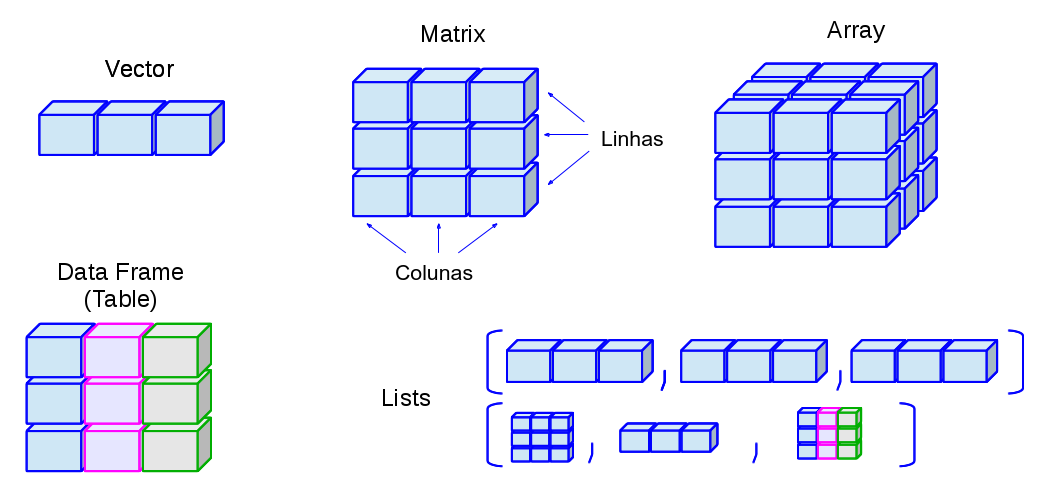
\includegraphics[width=1\linewidth]{images/dataStructuresR} \caption{Principais estruturas de dados no R.}\label{fig:fig-estrut-dados}
\end{figure}

\section{Vetor}\label{vetor}

Um vetor é uma coleção de elementos. Os vetores são amplamente usados e
compõem a estrutura básica de dados do R, por ser uma linguagem
vetorizada.

Os vetores podem ser de dois tipos: \textbf{vetores atômicos} e
\textbf{listas}.

\subsection{Vetores atômicos}\label{vetores-atomicos}

Os \textbf{vetores atômicos} são constituem a estrutura de dados mais
simples do R (como se fossem os átomos do R). Um vetor atômico é uma
coleção de elementos, em que todos são do mesmo tipo de dado (todos
\texttt{double}, ou \texttt{integer}, ou \texttt{logical}, etc).

Como linguagem vetorizada, as operações são aplicadas a cada elemento do
vetor automaticamente, sem a necessidade de laços (ou \emph{loopings})
ao longo do vetor. Esse conceito pode ser estranho para quem vem de
outras linguagens, mas é uma das grandes vantagens do R.

Vetores não tem dimensões, ou seja não existem é um vetor linha ou vetor
coluna.

\subsubsection{Propriedades}\label{propriedades}

\begin{itemize}
\item
  \texttt{typeof()} para descobrir o tipo de dado
\item
  \texttt{length()} para descobrir o tamanho de um tipo de dado
\item
  \texttt{attributes} (informações acionais específicas do dado), entre
  eles o atributo mais comum está o \texttt{names()}.
\end{itemize}

\subsubsection{Criação}\label{criacao}

\textbf{Vetores atômicos} são geralmente criados com \texttt{c()},
abreviatura para o verbo \textbf{combinar ou concatenar}.

\begin{Shaded}
\begin{Highlighting}[]
\CommentTok{# vetor numérico}
\NormalTok{vetor_num <-}\StringTok{ }\KeywordTok{c}\NormalTok{(}\DecValTok{5}\NormalTok{, }\FloatTok{2.5}\NormalTok{, }\FloatTok{4.5}\NormalTok{)}
\CommentTok{# Note o sufixo L que distingue variaveis "double" de "integers"}
\NormalTok{vetor_int <-}\StringTok{ }\KeywordTok{c}\NormalTok{(1L, 6L, 10L)}
\CommentTok{# Vetor logico}
\NormalTok{vetor_log <-}\StringTok{ }\KeywordTok{c}\NormalTok{(}\OtherTok{TRUE}\NormalTok{, }\OtherTok{FALSE}\NormalTok{, }\OtherTok{TRUE}\NormalTok{, }\OtherTok{FALSE}\NormalTok{)}
\CommentTok{# Vetor de caracteres}
\NormalTok{vetor_char <-}\StringTok{ }\KeywordTok{c}\NormalTok{(}\StringTok{"Analise de dados"}\NormalTok{, }\StringTok{"ambientais com o R"}\NormalTok{)}
\end{Highlighting}
\end{Shaded}

Vetores atômicos podem ser criados a partir de outros vetores aninhados
entre si pela função \texttt{c()}.

\begin{Shaded}
\begin{Highlighting}[]
\NormalTok{v1 <-}\StringTok{ }\DecValTok{1} \CommentTok{# vetor com 1 elemento}
\NormalTok{v2 <-}\StringTok{ }\KeywordTok{c}\NormalTok{(}\DecValTok{2}\NormalTok{) }\CommentTok{# vetor com 1 elemento}
\NormalTok{v3 <-}\StringTok{ }\KeywordTok{c}\NormalTok{(}\DecValTok{4}\NormalTok{, }\DecValTok{6}\NormalTok{) }\CommentTok{# vetor com 2 elemento}
\end{Highlighting}
\end{Shaded}

Formas diferentes para criação de vetor que resultam num mesmo vetor:

\begin{Shaded}
\begin{Highlighting}[]
\NormalTok{(v_}\DecValTok{123}\NormalTok{ <-}\StringTok{ }\KeywordTok{c}\NormalTok{(v1, v2, v3))}
\CommentTok{#> [1] 1 2 4 6}
\NormalTok{(v_123a <-}\StringTok{ }\KeywordTok{c}\NormalTok{(}\DecValTok{1}\NormalTok{, }\KeywordTok{c}\NormalTok{(v2, v3)))}
\CommentTok{#> [1] 1 2 4 6}
\NormalTok{(v_123b <-}\StringTok{ }\KeywordTok{c}\NormalTok{(vetor_num, }\KeywordTok{c}\NormalTok{(v1, v2), v3))}
\CommentTok{#> [1] 5.0 2.5 4.5 1.0 2.0 4.0 6.0}
\NormalTok{v <-}\StringTok{ }\KeywordTok{c}\NormalTok{(}\DecValTok{1}\NormalTok{, }\DecValTok{2}\NormalTok{, }\DecValTok{4}\NormalTok{, }\DecValTok{6}\NormalTok{)}
\NormalTok{v}
\CommentTok{#> [1] 1 2 4 6}
\end{Highlighting}
\end{Shaded}

\subsubsection{Coerção de vetores}\label{coercao-de-vetores}

\begin{Shaded}
\begin{Highlighting}[]
\KeywordTok{c}\NormalTok{(}\StringTok{"a"}\NormalTok{, }\DecValTok{1}\NormalTok{)}
\CommentTok{#> [1] "a" "1"}
\KeywordTok{as.numeric}\NormalTok{(}\KeywordTok{c}\NormalTok{(}\OtherTok{FALSE}\NormalTok{, }\OtherTok{FALSE}\NormalTok{, }\OtherTok{TRUE}\NormalTok{))}
\CommentTok{#> [1] 0 0 1}
\end{Highlighting}
\end{Shaded}

Você pode manualmente forçar um tipo de vetor para outro usando funções
de coerção: \texttt{as.character()},
\texttt{as.double()},\texttt{as.integer()}, \texttt{as.logical()}.
Coerção frequentemente acontece automaticamente, mas geralmente será
mostrada uma mensagem quando ocorrer.

Vamos usar a coerção no seguinte caso. Imagine um vetor com valores de
chuva mensal de um ano e outro vetor com os meses do ano. Note a
diferença da forma como criamos o vetor \texttt{meses} e o vetor
\texttt{months}. Como descobrir o número de meses sem chuva nesse ano?

\begin{Shaded}
\begin{Highlighting}[]
\CommentTok{# vetor com nomes criados com 1 comando}
\NormalTok{meses <-}\StringTok{ }\KeywordTok{c}\NormalTok{(}
  \DataTypeTok{jan =} \DecValTok{1}\NormalTok{, }\DataTypeTok{fev =} \DecValTok{2}\NormalTok{, }\DataTypeTok{mar =} \DecValTok{3}\NormalTok{, }\DataTypeTok{abr =} \DecValTok{4}\NormalTok{, }\DataTypeTok{mai =} \DecValTok{5}\NormalTok{, }\DataTypeTok{jun =} \DecValTok{6}\NormalTok{,}
  \DataTypeTok{jul =} \DecValTok{7}\NormalTok{, }\DataTypeTok{ago =} \DecValTok{8}\NormalTok{, }\DataTypeTok{set =} \DecValTok{9}\NormalTok{, }\DataTypeTok{out =} \DecValTok{10}\NormalTok{, }\DataTypeTok{nov =} \DecValTok{11}\NormalTok{, }\DataTypeTok{dez =} \DecValTok{12}
\NormalTok{)}
\NormalTok{meses}
\CommentTok{#> jan fev mar abr mai jun jul ago set out nov dez }
\CommentTok{#>   1   2   3   4   5   6   7   8   9  10  11  12}
\CommentTok{# vetor definido e depois adiciona-se o nome das variáveis}
\NormalTok{months <-}\StringTok{ }\KeywordTok{c}\NormalTok{(}\DecValTok{1}\NormalTok{, }\DecValTok{2}\NormalTok{, }\DecValTok{3}\NormalTok{, }\DecValTok{4}\NormalTok{, }\DecValTok{5}\NormalTok{, }\DecValTok{6}\NormalTok{, }\DecValTok{7}\NormalTok{, }\DecValTok{8}\NormalTok{, }\DecValTok{9}\NormalTok{, }\DecValTok{10}\NormalTok{, }\DecValTok{11}\NormalTok{, }\DecValTok{12}\NormalTok{)}
\KeywordTok{names}\NormalTok{(months) <-}\StringTok{ }\KeywordTok{c}\NormalTok{(}\StringTok{"Jan"}\NormalTok{, }\StringTok{"Feb"}\NormalTok{, }\StringTok{"Mar"}\NormalTok{, }\StringTok{"Apr"}\NormalTok{, }\StringTok{"May"}\NormalTok{, }\StringTok{"Jun"}\NormalTok{, }\StringTok{"Jul"}\NormalTok{, }\StringTok{"Aug"}\NormalTok{, }\StringTok{"Sep"}\NormalTok{, }\StringTok{"Oct"}\NormalTok{, }\StringTok{"Nov"}\NormalTok{, }\StringTok{"Dec"}\NormalTok{)}
\NormalTok{months}
\CommentTok{#> Jan Feb Mar Apr May Jun Jul Aug Sep Oct Nov Dec }
\CommentTok{#>   1   2   3   4   5   6   7   8   9  10  11  12}
\CommentTok{# o atibuto mais comum de um vetor}
\KeywordTok{attributes}\NormalTok{(meses)}
\CommentTok{#> $names}
\CommentTok{#>  [1] "jan" "fev" "mar" "abr" "mai" "jun" "jul" "ago" "set" "out" "nov"}
\CommentTok{#> [12] "dez"}
\KeywordTok{length}\NormalTok{(meses)}
\CommentTok{#> [1] 12}
\CommentTok{# Vetor com dados de prec}
\NormalTok{chuva <-}\StringTok{ }\KeywordTok{c}\NormalTok{(}\DecValTok{100}\NormalTok{, }\DecValTok{0}\NormalTok{, }\DecValTok{20}\NormalTok{, }\DecValTok{140}\NormalTok{, }\DecValTok{110}\NormalTok{, }\DecValTok{50}\NormalTok{, }\DecValTok{90}\NormalTok{, }\DecValTok{0}\NormalTok{, }\DecValTok{0}\NormalTok{, }\DecValTok{10}\NormalTok{, }\DecValTok{0}\NormalTok{, }\DecValTok{6}\NormalTok{)}
\KeywordTok{length}\NormalTok{(chuva)}
\CommentTok{#> [1] 12}
\CommentTok{# quando nao choveu?}
\NormalTok{seco <-}\StringTok{ }\NormalTok{chuva }\OperatorTok{==}\StringTok{ }\DecValTok{0}
\NormalTok{seco}
\CommentTok{#>  [1] FALSE  TRUE FALSE FALSE FALSE FALSE FALSE  TRUE  TRUE FALSE  TRUE}
\CommentTok{#> [12] FALSE}
\CommentTok{# coerção de lógico para numérico}
\NormalTok{seco01 <-}\StringTok{ }\KeywordTok{as.numeric}\NormalTok{(seco)}
\CommentTok{# seco01 <- as.integer(seco)}
\NormalTok{seco01}
\CommentTok{#>  [1] 0 1 0 0 0 0 0 1 1 0 1 0}
\CommentTok{# total de meses secos no ano}
\KeywordTok{sum}\NormalTok{(seco01)}
\CommentTok{#> [1] 4}
\CommentTok{# também funciona com vetores lógicos}
\KeywordTok{sum}\NormalTok{(seco)}
\CommentTok{#> [1] 4}
\end{Highlighting}
\end{Shaded}

\subsubsection{Nomeando vetores}\label{nomeando-vetores}

Nós podemos nomear um vetor de 3 formas:

\begin{itemize}
\item
  Durante a criação
\item
  Modificando um vetor
\item
  Criando um vetor modificado
\end{itemize}

Nomes devem ser únicos (sem repetições), porque para filtragem de
elementos de um vetor ou a seleção de um subconjunto (razão pela qual
usam-se os \texttt{names}) retornará somente o primeiro elemento que
tiver nome repetido.

\begin{Shaded}
\begin{Highlighting}[]
\CommentTok{# Durante a criação:}
\NormalTok{x <-}\StringTok{ }\KeywordTok{c}\NormalTok{(}\DataTypeTok{a =} \DecValTok{1}\NormalTok{, }\DataTypeTok{b =} \DecValTok{2}\NormalTok{, }\DataTypeTok{c =} \DecValTok{3}\NormalTok{)}
\NormalTok{x}
\CommentTok{#> a b c }
\CommentTok{#> 1 2 3}
\CommentTok{# Modificando um vetor:}
\NormalTok{x <-}\StringTok{ }\DecValTok{1}\OperatorTok{:}\DecValTok{3}
\KeywordTok{names}\NormalTok{(x) <-}\StringTok{ }\KeywordTok{c}\NormalTok{(}\StringTok{"a"}\NormalTok{, }\StringTok{"b"}\NormalTok{, }\StringTok{"c"}\NormalTok{)}
\NormalTok{x}
\CommentTok{#> a b c }
\CommentTok{#> 1 2 3}
\CommentTok{# Criando um vetor modificado}
\NormalTok{x <-}\StringTok{ }\KeywordTok{setNames}\NormalTok{(}\DecValTok{1}\OperatorTok{:}\DecValTok{3}\NormalTok{, }\KeywordTok{c}\NormalTok{(}\StringTok{"a"}\NormalTok{, }\StringTok{"b"}\NormalTok{, }\StringTok{"c"}\NormalTok{))}
\NormalTok{x}
\CommentTok{#> a b c }
\CommentTok{#> 1 2 3}
\end{Highlighting}
\end{Shaded}

Nem todos elementos precisam ter nomes. Se os nomes são faltantes,
\texttt{names()} retornará um string vazia (``'') para aqueles
elementos. Se todos forem faltantes, \texttt{names()} retornará
\texttt{NULL}.

\begin{Shaded}
\begin{Highlighting}[]
\NormalTok{y <-}\StringTok{ }\KeywordTok{c}\NormalTok{(}\DataTypeTok{a =} \DecValTok{1}\NormalTok{, }\DecValTok{2}\NormalTok{, }\DecValTok{3}\NormalTok{)}
\KeywordTok{names}\NormalTok{(y)}
\CommentTok{#> [1] "a" ""  ""}
\NormalTok{z <-}\StringTok{ }\KeywordTok{c}\NormalTok{(}\DecValTok{1}\NormalTok{, }\DecValTok{2}\NormalTok{, }\DecValTok{3}\NormalTok{)}
\KeywordTok{names}\NormalTok{(z)}
\CommentTok{#> NULL}
\end{Highlighting}
\end{Shaded}

Podemos criar um vetor sem nomes usando a função \texttt{unname(x)}, ou
remover \texttt{names} com \texttt{names(x)\ \textless{}-\ NULL}.

\begin{Shaded}
\begin{Highlighting}[]
\NormalTok{a <-}\StringTok{ }\KeywordTok{c}\NormalTok{(}\DataTypeTok{dia1 =} \DecValTok{12}\NormalTok{, }\DataTypeTok{dia2 =} \DecValTok{20}\NormalTok{, }\DataTypeTok{dia3 =} \DecValTok{10}\NormalTok{)}
\NormalTok{a}
\CommentTok{#> dia1 dia2 dia3 }
\CommentTok{#>   12   20   10}
\KeywordTok{names}\NormalTok{(a)}
\CommentTok{#> [1] "dia1" "dia2" "dia3"}
\NormalTok{a_sn <-}\StringTok{ }\KeywordTok{unname}\NormalTok{(a)}
\NormalTok{a_sn}
\CommentTok{#> [1] 12 20 10}
\KeywordTok{names}\NormalTok{(a_sn)}
\CommentTok{#> NULL}
\end{Highlighting}
\end{Shaded}

\subsection{Operações com vetores}\label{operacoes-com-vetores}

Para multiplicar cada elemento de um vetor por um valor é usar o
operador de multiplicação (*). O mesmo procedimento se aplica as demais
operações de soma, subtração, divisão, exponenciação e etc.

\begin{Shaded}
\begin{Highlighting}[]
\NormalTok{x <-}\StringTok{ }\DecValTok{1}\OperatorTok{:}\DecValTok{10}
\NormalTok{x }\OperatorTok{*}\StringTok{ }\DecValTok{3}
\CommentTok{#>  [1]  3  6  9 12 15 18 21 24 27 30}
\NormalTok{x }\OperatorTok{+}\StringTok{ }\DecValTok{2}
\CommentTok{#>  [1]  3  4  5  6  7  8  9 10 11 12}
\NormalTok{x }\OperatorTok{-}\StringTok{ }\DecValTok{3}
\CommentTok{#>  [1] -2 -1  0  1  2  3  4  5  6  7}
\NormalTok{x }\OperatorTok{/}\StringTok{ }\DecValTok{4}
\CommentTok{#>  [1] 0.25 0.50 0.75 1.00 1.25 1.50 1.75 2.00 2.25 2.50}
\DecValTok{2} \OperatorTok{^}\StringTok{ }\NormalTok{(x }\OperatorTok{/}\StringTok{ }\DecValTok{4}\NormalTok{)}
\CommentTok{#>  [1] 1.189207 1.414214 1.681793 2.000000 2.378414 2.828427 3.363586}
\CommentTok{#>  [8] 4.000000 4.756828 5.656854}
\NormalTok{x }\OperatorTok{^}\StringTok{ }\DecValTok{2}
\CommentTok{#>  [1]   1   4   9  16  25  36  49  64  81 100}
\KeywordTok{sqrt}\NormalTok{(x)}
\CommentTok{#>  [1] 1.000000 1.414214 1.732051 2.000000 2.236068 2.449490 2.645751}
\CommentTok{#>  [8] 2.828427 3.000000 3.162278}
\end{Highlighting}
\end{Shaded}

Operações vetoriais podem ser estendidas para mais de um vetor.

\begin{Shaded}
\begin{Highlighting}[]
\CommentTok{# criando 2 vetores de mesmo tamanho}
\NormalTok{x <-}\StringTok{ }\DecValTok{1}\OperatorTok{:}\DecValTok{10}
\NormalTok{y <-}\StringTok{ }\OperatorTok{-}\DecValTok{5}\OperatorTok{:}\DecValTok{4}
\CommentTok{# somando-os}
\NormalTok{x }\OperatorTok{+}\StringTok{ }\NormalTok{y}
\CommentTok{#>  [1] -4 -2  0  2  4  6  8 10 12 14}
\NormalTok{x }\OperatorTok{-}\StringTok{ }\NormalTok{y}
\CommentTok{#>  [1] 6 6 6 6 6 6 6 6 6 6}
\NormalTok{x }\OperatorTok{*}\StringTok{ }\NormalTok{y}
\CommentTok{#>  [1] -5 -8 -9 -8 -5  0  7 16 27 40}
\NormalTok{x }\OperatorTok{/}\StringTok{ }\NormalTok{y}
\CommentTok{#>  [1] -0.2 -0.5 -1.0 -2.0 -5.0  Inf  7.0  4.0  3.0  2.5}
\NormalTok{x }\OperatorTok{^}\StringTok{ }\NormalTok{y}
\CommentTok{#>  [1] 1.000000e+00 6.250000e-02 3.703704e-02 6.250000e-02 2.000000e-01}
\CommentTok{#>  [6] 1.000000e+00 7.000000e+00 6.400000e+01 7.290000e+02 1.000000e+04}
\DecValTok{2} \OperatorTok{^}\StringTok{ }\NormalTok{x}
\CommentTok{#>  [1]    2    4    8   16   32   64  128  256  512 1024}
\NormalTok{x }\OperatorTok\StringTok{ }\NormalTok{y}
\CommentTok{#>  [1] -4 -2  0  0  0 NA  0  0  0  2}
\CommentTok{# tamanho dos vetores}
\KeywordTok{length}\NormalTok{(x)}
\CommentTok{#> [1] 10}
\KeywordTok{length}\NormalTok{(y)}
\CommentTok{#> [1] 10}
\KeywordTok{length}\NormalTok{(x }\OperatorTok{+}\StringTok{ }\NormalTok{y)}
\CommentTok{#> [1] 10}
\end{Highlighting}
\end{Shaded}

Uma peculiaridade do R é o tratamento de operações com vetores de
tamanhos diferentes. O vetor menor é reciclado, de forma que seus
elementos sejam repetidos em ordem até atingirem o tamanho do vetor mais
longo envolvido na operação.

\begin{Shaded}
\begin{Highlighting}[]
\NormalTok{v1 <-}\StringTok{ }\KeywordTok{c}\NormalTok{(}\DecValTok{3}\NormalTok{, }\DecValTok{5}\NormalTok{, }\DecValTok{88}\NormalTok{, }\DecValTok{90}\NormalTok{)}
\NormalTok{v2 <-}\StringTok{ }\KeywordTok{c}\NormalTok{(}\DecValTok{2}\NormalTok{, }\DecValTok{1}\NormalTok{)}
\NormalTok{v1 }\OperatorTok{+}\StringTok{ }\NormalTok{v2}
\CommentTok{#> [1]  5  6 90 91}
\end{Highlighting}
\end{Shaded}

Se o vetor mais longo não é múltiplo do mais curto, o R imprime um
aviso.

\begin{Shaded}
\begin{Highlighting}[]
\NormalTok{v1 <-}\StringTok{ }\KeywordTok{c}\NormalTok{(}\DecValTok{3}\NormalTok{, }\DecValTok{5}\NormalTok{, }\DecValTok{88}\NormalTok{, }\DecValTok{90}\NormalTok{)}
\NormalTok{v2 <-}\StringTok{ }\KeywordTok{c}\NormalTok{(}\DecValTok{2}\NormalTok{, }\DecValTok{1}\NormalTok{, }\DecValTok{3}\NormalTok{)}
\NormalTok{v1 }\OperatorTok{+}\StringTok{ }\NormalTok{v2}
\CommentTok{#> Warning in v1 + v2: longer object length is not a multiple of shorter}
\CommentTok{#> object length}
\CommentTok{#> [1]  5  6 91 92}
\end{Highlighting}
\end{Shaded}

A reciclagem é intrinsecamente usada em operações envolvendo vetores.

\begin{Shaded}
\begin{Highlighting}[]
\NormalTok{v1}
\CommentTok{#> [1]  3  5 88 90}
\NormalTok{cte <-}\StringTok{ }\DecValTok{4}
\NormalTok{v1 }\OperatorTok{*}\StringTok{ }\NormalTok{cte}
\CommentTok{#> [1]  12  20 352 360}
\end{Highlighting}
\end{Shaded}

O número 4 nesse caso é reciclado 4 vezes e então multiplicado por cada
elemento do vetor \texttt{v1}. Avisos e erros:

\begin{Shaded}
\begin{Highlighting}[]
\NormalTok{v1 <-}\StringTok{ }\KeywordTok{c}\NormalTok{(}\DecValTok{3}\NormalTok{, }\DecValTok{5}\NormalTok{, }\DecValTok{88}\NormalTok{, }\DecValTok{90}\NormalTok{)}
\KeywordTok{srt}\NormalTok{(v1)}
\CommentTok{#> Error in srt(v1): could not find function "srt"}
\KeywordTok{sqrt}\NormalTok{(}\OperatorTok{-}\NormalTok{v1)}
\CommentTok{#> Warning in sqrt(-v1): NaNs produced}
\CommentTok{#> [1] NaN NaN NaN NaN}
\end{Highlighting}
\end{Shaded}

Comparações também funcionam com vetores.

\begin{Shaded}
\begin{Highlighting}[]
\NormalTok{x }\OperatorTok{<=}\StringTok{ }\DecValTok{5}
\CommentTok{#>  [1]  TRUE  TRUE  TRUE  TRUE  TRUE FALSE FALSE FALSE FALSE FALSE}
\NormalTok{x }\OperatorTok{>}\StringTok{ }\NormalTok{y}
\CommentTok{#>  [1] TRUE TRUE TRUE TRUE TRUE TRUE TRUE TRUE TRUE TRUE}
\NormalTok{x }\OperatorTok{<}\StringTok{ }\NormalTok{y}
\CommentTok{#>  [1] FALSE FALSE FALSE FALSE FALSE FALSE FALSE FALSE FALSE FALSE}
\end{Highlighting}
\end{Shaded}

Entre os operadores lógicos vistos (Tabela \ref{tab:oper-logic}) alguns
deles não foram aplicados em exemplos. Vamos então usar o operador
\texttt{\%in\%} para verificar se um vetor está contido parcial ou
totalmente em outro vetor.

\begin{Shaded}
\begin{Highlighting}[]
\CommentTok{# operador está contido em}
\DecValTok{2}\OperatorTok{:}\DecValTok{4} \OperatorTok\StringTok{ }\NormalTok{x}
\CommentTok{#> [1] TRUE TRUE TRUE}
\CommentTok{# 2:4 são elementos de x?}
\KeywordTok{is.element}\NormalTok{(}\DecValTok{2}\OperatorTok{:}\DecValTok{4}\NormalTok{, x)}
\CommentTok{#> [1] TRUE TRUE TRUE}
\end{Highlighting}
\end{Shaded}

A função \texttt{nchar()} também funciona sobre cada elemento do vetor.
Esse é mais um exemplo de função vetorizada do R.

\begin{Shaded}
\begin{Highlighting}[]
\KeywordTok{nchar}\NormalTok{(month.name)}
\CommentTok{#>  [1] 7 8 5 5 3 4 4 6 9 7 8 8}
\KeywordTok{nchar}\NormalTok{(y)}
\CommentTok{#>  [1] 2 2 2 2 2 1 1 1 1 1}
\end{Highlighting}
\end{Shaded}

\subsubsection{\texorpdfstring{Operadores \texttt{any} e
\texttt{all}}{Operadores any e all}}\label{operadores-any-e-all}

\begin{Shaded}
\begin{Highlighting}[]
\NormalTok{vetor <-}\StringTok{ }\KeywordTok{c}\NormalTok{(}\DecValTok{0}\NormalTok{, }\DecValTok{1}\NormalTok{, }\OperatorTok{-}\DecValTok{1}\NormalTok{, }\OperatorTok{-}\DecValTok{2}\NormalTok{, }\DecValTok{3}\NormalTok{, }\DecValTok{5}\NormalTok{, }\OperatorTok{-}\DecValTok{5}\NormalTok{)}
\KeywordTok{all}\NormalTok{(vetor }\OperatorTok{<}\StringTok{ }\DecValTok{0}\NormalTok{)  }\CommentTok{# todas as posições são maiores que 0 ?}
\CommentTok{#> [1] FALSE}
\KeywordTok{any}\NormalTok{(vetor }\OperatorTok{>}\StringTok{ }\DecValTok{0}\NormalTok{)  }\CommentTok{# alguma posição é maior que 0?}
\CommentTok{#> [1] TRUE}
\end{Highlighting}
\end{Shaded}

Ambas as funções sintetizam a informação:

\begin{itemize}
\tightlist
\item
  \texttt{all()} verifica se a condição avaliada é válida para todos
  elementos do vetor;
\item
  \texttt{any()} verifica se a condição avaliada é válida para pelo
  menos um dos elementos do vetor;
\end{itemize}

As funções fornecem um único valor (vetor lógico de tamanho 1) para
resumir ou descrever o resultado da condição aplicada ao vetor.

\subsection{Sequências}\label{sequencias}

Vimos nas seções anteriores que é muito simples criar sequências de
números inteiros com o operador \texttt{:}. Nesta seção veremos outras
formas de gerar sequências, como uma sequência de números não inteiros e
sequências de números repetidos.

\subsubsection{Sequências de números
inteiros}\label{sequencias-de-numeros-inteiros}

Sequências de números formam um vetor. Há diversas formas de se gerar
sequências no R. Para gerar uma sequência de 1 até 365, em vez de
escrevermos cada número e combiná-los usando \texttt{c(1,2,3,...,365)},
podemos usar o operador \texttt{:} da seguinte forma:

\begin{Shaded}
\begin{Highlighting}[]
\CommentTok{# dias do ano}
\NormalTok{dda <-}\StringTok{ }\DecValTok{1}\OperatorTok{:}\DecValTok{365}
\NormalTok{dda}
\CommentTok{#>   [1]   1   2   3   4   5   6   7   8   9  10  11  12  13  14  15  16  17}
\CommentTok{#>  [18]  18  19  20  21  22  23  24  25  26  27  28  29  30  31  32  33  34}
\CommentTok{#>  [35]  35  36  37  38  39  40  41  42  43  44  45  46  47  48  49  50  51}
\CommentTok{#>  [52]  52  53  54  55  56  57  58  59  60  61  62  63  64  65  66  67  68}
\CommentTok{#>  [69]  69  70  71  72  73  74  75  76  77  78  79  80  81  82  83  84  85}
\CommentTok{#>  [86]  86  87  88  89  90  91  92  93  94  95  96  97  98  99 100 101 102}
\CommentTok{#> [103] 103 104 105 106 107 108 109 110 111 112 113 114 115 116 117 118 119}
\CommentTok{#> [120] 120 121 122 123 124 125 126 127 128 129 130 131 132 133 134 135 136}
\CommentTok{#> [137] 137 138 139 140 141 142 143 144 145 146 147 148 149 150 151 152 153}
\CommentTok{#> [154] 154 155 156 157 158 159 160 161 162 163 164 165 166 167 168 169 170}
\CommentTok{#> [171] 171 172 173 174 175 176 177 178 179 180 181 182 183 184 185 186 187}
\CommentTok{#> [188] 188 189 190 191 192 193 194 195 196 197 198 199 200 201 202 203 204}
\CommentTok{#> [205] 205 206 207 208 209 210 211 212 213 214 215 216 217 218 219 220 221}
\CommentTok{#> [222] 222 223 224 225 226 227 228 229 230 231 232 233 234 235 236 237 238}
\CommentTok{#> [239] 239 240 241 242 243 244 245 246 247 248 249 250 251 252 253 254 255}
\CommentTok{#> [256] 256 257 258 259 260 261 262 263 264 265 266 267 268 269 270 271 272}
\CommentTok{#> [273] 273 274 275 276 277 278 279 280 281 282 283 284 285 286 287 288 289}
\CommentTok{#> [290] 290 291 292 293 294 295 296 297 298 299 300 301 302 303 304 305 306}
\CommentTok{#> [307] 307 308 309 310 311 312 313 314 315 316 317 318 319 320 321 322 323}
\CommentTok{#> [324] 324 325 326 327 328 329 330 331 332 333 334 335 336 337 338 339 340}
\CommentTok{#> [341] 341 342 343 344 345 346 347 348 349 350 351 352 353 354 355 356 357}
\CommentTok{#> [358] 358 359 360 361 362 363 364 365}
\CommentTok{# sequencia de anos}
\NormalTok{anos <-}\StringTok{ }\DecValTok{1961}\OperatorTok{:}\DecValTok{1990}
\NormalTok{anos}
\CommentTok{#>  [1] 1961 1962 1963 1964 1965 1966 1967 1968 1969 1970 1971 1972 1973 1974}
\CommentTok{#> [15] 1975 1976 1977 1978 1979 1980 1981 1982 1983 1984 1985 1986 1987 1988}
\CommentTok{#> [29] 1989 1990}
\CommentTok{# sequencia de inteiros decrescente}
\NormalTok{si_dec <-}\StringTok{ }\DecValTok{10}\OperatorTok{:-}\DecValTok{10}
\NormalTok{si_dec}
\CommentTok{#>  [1]  10   9   8   7   6   5   4   3   2   1   0  -1  -2  -3  -4  -5  -6}
\CommentTok{#> [18]  -7  -8  -9 -10}
\CommentTok{# sequencia de numeros não inteiros}
\NormalTok{seqn <-}\StringTok{ }\FloatTok{1.5}\OperatorTok{:}\DecValTok{10}
\NormalTok{seqn}
\CommentTok{#> [1] 1.5 2.5 3.5 4.5 5.5 6.5 7.5 8.5 9.5}
\KeywordTok{c}\NormalTok{(seqn, }\DecValTok{10}\NormalTok{)}
\CommentTok{#>  [1]  1.5  2.5  3.5  4.5  5.5  6.5  7.5  8.5  9.5 10.0}
\end{Highlighting}
\end{Shaded}

\subsubsection{Sequências de números não
inteiros}\label{sequencias-de-numeros-nao-inteiros}

Mas para gerar uma sequencia de números não inteiros há uma função
específica para tal tarefa.

\begin{Shaded}
\begin{Highlighting}[]
\CommentTok{# igual a c(snum, 10), mas usando o seq}
\NormalTok{(snum_b <-}\StringTok{ }\KeywordTok{seq}\NormalTok{(}\DataTypeTok{from =} \FloatTok{1.5}\NormalTok{, }\DataTypeTok{to =} \DecValTok{10}\NormalTok{, }\DataTypeTok{by =} \FloatTok{0.5}\NormalTok{))}
\CommentTok{#>  [1]  1.5  2.0  2.5  3.0  3.5  4.0  4.5  5.0  5.5  6.0  6.5  7.0  7.5  8.0}
\CommentTok{#> [15]  8.5  9.0  9.5 10.0}
\end{Highlighting}
\end{Shaded}

Exemplos de sequência de anos, meses e dias.

\begin{Shaded}
\begin{Highlighting}[]
\CommentTok{# vetor com de anos decimais (2 valores por dia)}
\NormalTok{anos_dec <-}\StringTok{ }\KeywordTok{seq}\NormalTok{(}\DecValTok{2010}\NormalTok{, }\DecValTok{2011}\NormalTok{, }\DataTypeTok{length.out =} \DecValTok{365} \OperatorTok{*}\StringTok{ }\DecValTok{2}\NormalTok{)}
\CommentTok{# para ver só o início do vetor ao invés de todo o vetor}
\KeywordTok{head}\NormalTok{(anos_dec)}
\CommentTok{#> [1] 2010.000 2010.001 2010.003 2010.004 2010.005 2010.007}
\CommentTok{# mas não dá pra ver a parte decimal, vamos alterar as opções}
\CommentTok{# aumentando as casas decimais}
\KeywordTok{options}\NormalTok{(}\DataTypeTok{digits =} \DecValTok{6}\NormalTok{)}
\CommentTok{# verifique agora}
\KeywordTok{head}\NormalTok{(anos_dec)}
\CommentTok{#> [1] 2010.00 2010.00 2010.00 2010.00 2010.01 2010.01}
\CommentTok{# só os primeiros 30 elementos}
\KeywordTok{head}\NormalTok{(anos_dec, }\DecValTok{30}\NormalTok{)}
\CommentTok{#>  [1] 2010.00 2010.00 2010.00 2010.00 2010.01 2010.01 2010.01 2010.01}
\CommentTok{#>  [9] 2010.01 2010.01 2010.01 2010.02 2010.02 2010.02 2010.02 2010.02}
\CommentTok{#> [17] 2010.02 2010.02 2010.02 2010.03 2010.03 2010.03 2010.03 2010.03}
\CommentTok{#> [25] 2010.03 2010.03 2010.04 2010.04 2010.04 2010.04}
\CommentTok{# para ver só o final do vetor yrFrac}
\KeywordTok{tail}\NormalTok{(anos_dec)}
\CommentTok{#> [1] 2010.99 2010.99 2011.00 2011.00 2011.00 2011.00}
\CommentTok{# para ver só os último 50 elementos do yrFrac}
\KeywordTok{tail}\NormalTok{(anos_dec, }\DecValTok{50}\NormalTok{)}
\CommentTok{#>  [1] 2010.93 2010.93 2010.94 2010.94 2010.94 2010.94 2010.94 2010.94}
\CommentTok{#>  [9] 2010.94 2010.95 2010.95 2010.95 2010.95 2010.95 2010.95 2010.95}
\CommentTok{#> [17] 2010.95 2010.96 2010.96 2010.96 2010.96 2010.96 2010.96 2010.96}
\CommentTok{#> [25] 2010.97 2010.97 2010.97 2010.97 2010.97 2010.97 2010.97 2010.98}
\CommentTok{#> [33] 2010.98 2010.98 2010.98 2010.98 2010.98 2010.98 2010.98 2010.99}
\CommentTok{#> [41] 2010.99 2010.99 2010.99 2010.99 2010.99 2010.99 2011.00 2011.00}
\CommentTok{#> [49] 2011.00 2011.00}
\CommentTok{# pentadas}
\NormalTok{pent <-}\StringTok{ }\KeywordTok{seq}\NormalTok{(}\DataTypeTok{from =} \DecValTok{1}\NormalTok{, }\DataTypeTok{to =} \DecValTok{365}\NormalTok{, }\DataTypeTok{by =} \DecValTok{5}\NormalTok{)}
\CommentTok{# dencendios}
\NormalTok{decd <-}\StringTok{ }\KeywordTok{seq}\NormalTok{(}\DataTypeTok{from =} \DecValTok{1}\NormalTok{, }\DataTypeTok{to =} \DecValTok{365}\NormalTok{, }\DataTypeTok{by =} \DecValTok{10}\NormalTok{)}
\CommentTok{# fracoes de dia}
\NormalTok{frac_d30mn <-}\StringTok{ }\KeywordTok{seq}\NormalTok{(}\DecValTok{0}\NormalTok{, }\DecValTok{365}\NormalTok{, }\DataTypeTok{length.out =} \DecValTok{365} \OperatorTok{*}\StringTok{ }\DecValTok{48}\NormalTok{) }\OperatorTok{+}\StringTok{ }\DecValTok{1}
\KeywordTok{head}\NormalTok{(frac_d30mn, }\DecValTok{48} \OperatorTok{*}\StringTok{ }\DecValTok{2}\NormalTok{)}
\CommentTok{#>  [1] 1.00000 1.02083 1.04167 1.06250 1.08334 1.10417 1.12501 1.14584}
\CommentTok{#>  [9] 1.16668 1.18751 1.20835 1.22918 1.25001 1.27085 1.29168 1.31252}
\CommentTok{#> [17] 1.33335 1.35419 1.37502 1.39586 1.41669 1.43752 1.45836 1.47919}
\CommentTok{#> [25] 1.50003 1.52086 1.54170 1.56253 1.58337 1.60420 1.62504 1.64587}
\CommentTok{#> [33] 1.66670 1.68754 1.70837 1.72921 1.75004 1.77088 1.79171 1.81255}
\CommentTok{#> [41] 1.83338 1.85422 1.87505 1.89588 1.91672 1.93755 1.95839 1.97922}
\CommentTok{#> [49] 2.00006 2.02089 2.04173 2.06256 2.08340 2.10423 2.12506 2.14590}
\CommentTok{#> [57] 2.16673 2.18757 2.20840 2.22924 2.25007 2.27091 2.29174 2.31257}
\CommentTok{#> [65] 2.33341 2.35424 2.37508 2.39591 2.41675 2.43758 2.45842 2.47925}
\CommentTok{#> [73] 2.50009 2.52092 2.54175 2.56259 2.58342 2.60426 2.62509 2.64593}
\CommentTok{#> [81] 2.66676 2.68760 2.70843 2.72927 2.75010 2.77093 2.79177 2.81260}
\CommentTok{#> [89] 2.83344 2.85427 2.87511 2.89594 2.91678 2.93761 2.95845 2.97928}
\KeywordTok{tail}\NormalTok{(frac_d30mn, }\DecValTok{48} \OperatorTok{*}\StringTok{ }\DecValTok{2}\NormalTok{)}
\CommentTok{#>  [1] 364.021 364.042 364.062 364.083 364.104 364.125 364.146 364.167}
\CommentTok{#>  [9] 364.187 364.208 364.229 364.250 364.271 364.292 364.312 364.333}
\CommentTok{#> [17] 364.354 364.375 364.396 364.417 364.437 364.458 364.479 364.500}
\CommentTok{#> [25] 364.521 364.542 364.562 364.583 364.604 364.625 364.646 364.667}
\CommentTok{#> [33] 364.687 364.708 364.729 364.750 364.771 364.792 364.812 364.833}
\CommentTok{#> [41] 364.854 364.875 364.896 364.917 364.937 364.958 364.979 365.000}
\CommentTok{#> [49] 365.021 365.042 365.062 365.083 365.104 365.125 365.146 365.167}
\CommentTok{#> [57] 365.187 365.208 365.229 365.250 365.271 365.292 365.312 365.333}
\CommentTok{#> [65] 365.354 365.375 365.396 365.417 365.437 365.458 365.479 365.500}
\CommentTok{#> [73] 365.521 365.542 365.562 365.583 365.604 365.625 365.646 365.667}
\CommentTok{#> [81] 365.687 365.708 365.729 365.750 365.771 365.792 365.812 365.833}
\CommentTok{#> [89] 365.854 365.875 365.896 365.917 365.937 365.958 365.979 366.000}
\CommentTok{# diferentes funções para gerar uma sequência}
\NormalTok{an <-}\StringTok{ }\KeywordTok{c}\NormalTok{(}\DecValTok{1}\NormalTok{, }\DecValTok{7}\NormalTok{, }\DecValTok{2}\NormalTok{, }\DecValTok{5}\NormalTok{, }\DecValTok{3}\NormalTok{, }\DecValTok{2}\NormalTok{)}
\CommentTok{# gerando uma sequencia a partir de um número}
\KeywordTok{seq_len}\NormalTok{(}\DataTypeTok{length.out =} \DecValTok{6}\NormalTok{)}
\CommentTok{#> [1] 1 2 3 4 5 6}
\CommentTok{# gerando uma sequência a partir de um número}
\KeywordTok{seq}\NormalTok{(}\DecValTok{6}\NormalTok{)}
\CommentTok{#> [1] 1 2 3 4 5 6}
\CommentTok{# de acordo com o tamanho do vetor gera-se uma sequencia}
\KeywordTok{seq}\NormalTok{(}\DataTypeTok{along =}\NormalTok{ an)}
\CommentTok{#> [1] 1 2 3 4 5 6}
\KeywordTok{seq}\NormalTok{(}\DataTypeTok{along =} \DecValTok{0}\NormalTok{) }\CommentTok{# ! melhor opção para gerar sequencias do tamanho do vetor}
\CommentTok{#> [1] 1}
\KeywordTok{seq}\NormalTok{(}\DecValTok{0}\NormalTok{) }\CommentTok{# ! cuidado, veja ?seq para entender a razão desse resultado inusitado}
\CommentTok{#> [1] 1 0}
\CommentTok{# conflito entre parâmetros}
\CommentTok{# a <-seq(from = -5, to = 5, by = 0.05, length.out=200)}
\NormalTok{s5by <-}\StringTok{ }\KeywordTok{seq}\NormalTok{(}\DataTypeTok{from =} \OperatorTok{-}\DecValTok{5}\NormalTok{, }\DataTypeTok{to =} \DecValTok{5}\NormalTok{, }\DataTypeTok{by =} \FloatTok{0.05}\NormalTok{)}
\KeywordTok{length}\NormalTok{(s5by)}
\CommentTok{#> [1] 201}
\KeywordTok{tail}\NormalTok{(s5by)}
\CommentTok{#> [1] 4.75 4.80 4.85 4.90 4.95 5.00}
\NormalTok{s5len <-}\StringTok{ }\KeywordTok{seq}\NormalTok{(}\DataTypeTok{from =} \OperatorTok{-}\DecValTok{5}\NormalTok{, }\DataTypeTok{to =} \DecValTok{5}\NormalTok{, }\DataTypeTok{length.out =} \DecValTok{200}\NormalTok{)}
\KeywordTok{length}\NormalTok{(s5len)}
\CommentTok{#> [1] 200}
\KeywordTok{tail}\NormalTok{(s5len)}
\CommentTok{#> [1] 4.74874 4.79899 4.84925 4.89950 4.94975 5.00000}
\end{Highlighting}
\end{Shaded}

\subsubsection{Sequências de números
repetidos}\label{sequencias-de-numeros-repetidos}

\begin{Shaded}
\begin{Highlighting}[]
\NormalTok{rep_t4 <-}\StringTok{ }\KeywordTok{rep}\NormalTok{(}\DecValTok{1}\OperatorTok{:}\DecValTok{2}\NormalTok{, }\DataTypeTok{times =} \DecValTok{4}\NormalTok{)}
\NormalTok{rep_t4}
\CommentTok{#> [1] 1 2 1 2 1 2 1 2}
\NormalTok{rep_e31 <-}\StringTok{ }\KeywordTok{rep}\NormalTok{(}\DecValTok{1}\OperatorTok{:}\DecValTok{12}\NormalTok{, }\DataTypeTok{each =} \DecValTok{31}\NormalTok{)}
\NormalTok{rep_e31}
\CommentTok{#>   [1]  1  1  1  1  1  1  1  1  1  1  1  1  1  1  1  1  1  1  1  1  1  1  1}
\CommentTok{#>  [24]  1  1  1  1  1  1  1  1  2  2  2  2  2  2  2  2  2  2  2  2  2  2  2}
\CommentTok{#>  [47]  2  2  2  2  2  2  2  2  2  2  2  2  2  2  2  2  3  3  3  3  3  3  3}
\CommentTok{#>  [70]  3  3  3  3  3  3  3  3  3  3  3  3  3  3  3  3  3  3  3  3  3  3  3}
\CommentTok{#>  [93]  3  4  4  4  4  4  4  4  4  4  4  4  4  4  4  4  4  4  4  4  4  4  4}
\CommentTok{#> [116]  4  4  4  4  4  4  4  4  4  5  5  5  5  5  5  5  5  5  5  5  5  5  5}
\CommentTok{#> [139]  5  5  5  5  5  5  5  5  5  5  5  5  5  5  5  5  5  6  6  6  6  6  6}
\CommentTok{#> [162]  6  6  6  6  6  6  6  6  6  6  6  6  6  6  6  6  6  6  6  6  6  6  6}
\CommentTok{#> [185]  6  6  7  7  7  7  7  7  7  7  7  7  7  7  7  7  7  7  7  7  7  7  7}
\CommentTok{#> [208]  7  7  7  7  7  7  7  7  7  7  8  8  8  8  8  8  8  8  8  8  8  8  8}
\CommentTok{#> [231]  8  8  8  8  8  8  8  8  8  8  8  8  8  8  8  8  8  8  9  9  9  9  9}
\CommentTok{#> [254]  9  9  9  9  9  9  9  9  9  9  9  9  9  9  9  9  9  9  9  9  9  9  9}
\CommentTok{#> [277]  9  9  9 10 10 10 10 10 10 10 10 10 10 10 10 10 10 10 10 10 10 10 10}
\CommentTok{#> [300] 10 10 10 10 10 10 10 10 10 10 10 11 11 11 11 11 11 11 11 11 11 11 11}
\CommentTok{#> [323] 11 11 11 11 11 11 11 11 11 11 11 11 11 11 11 11 11 11 11 12 12 12 12}
\CommentTok{#> [346] 12 12 12 12 12 12 12 12 12 12 12 12 12 12 12 12 12 12 12 12 12 12 12}
\CommentTok{#> [369] 12 12 12 12}
\NormalTok{rep_t13 <-}\StringTok{ }\KeywordTok{rep}\NormalTok{(}\KeywordTok{c}\NormalTok{(}\StringTok{"chuva"}\NormalTok{, }\StringTok{"sol"}\NormalTok{), }\DataTypeTok{times =} \KeywordTok{c}\NormalTok{(}\DecValTok{1}\NormalTok{, }\DecValTok{3}\NormalTok{))}
\NormalTok{rep_t13}
\CommentTok{#> [1] "chuva" "sol"   "sol"   "sol"}
\NormalTok{rep_t13_t4 <-}\StringTok{ }\KeywordTok{rep}\NormalTok{(}\KeywordTok{rep}\NormalTok{(}\KeywordTok{c}\NormalTok{(}\StringTok{"chuva"}\NormalTok{, }\StringTok{"sol"}\NormalTok{), }\DataTypeTok{times =} \KeywordTok{c}\NormalTok{(}\DecValTok{1}\NormalTok{, }\DecValTok{3}\NormalTok{)), }\DataTypeTok{times =} \DecValTok{4}\NormalTok{)}
\NormalTok{rep_t13_t4}
\CommentTok{#>  [1] "chuva" "sol"   "sol"   "sol"   "chuva" "sol"   "sol"   "sol"  }
\CommentTok{#>  [9] "chuva" "sol"   "sol"   "sol"   "chuva" "sol"   "sol"   "sol"}
\end{Highlighting}
\end{Shaded}

\subsection{Indexação de vetores}\label{index-vetores}

Os elementos de um vetor são indexados e para acessá-los usamos a
notação de índices do R.

Podemos selecionar partes de um vetor por números (posição do elemento),
caracteres (nome) e vetores lógicos.

Através do operador \texttt{{[}} podemos acessar ou filtrar elementos de
um vetor. O operador colchete \texttt{{[}} aplicado a um vetor retornará
um vetor.

Considere os seguintes vetores como exemplo:

\begin{Shaded}
\begin{Highlighting}[]
\CommentTok{# vetor de chuva mensal para um dado ano}
\NormalTok{prec <-}\StringTok{ }\KeywordTok{c}\NormalTok{(}\DecValTok{300}\NormalTok{, }\DecValTok{150}\NormalTok{, }\DecValTok{210}\NormalTok{, }\DecValTok{12}\NormalTok{, }\DecValTok{0}\NormalTok{, }\DecValTok{0}\NormalTok{, }\DecValTok{12}\NormalTok{, }\DecValTok{22}\NormalTok{, }\DecValTok{80}\NormalTok{, }\DecValTok{100}\NormalTok{, }\DecValTok{0}\NormalTok{, }\DecValTok{280}\NormalTok{)}
\NormalTok{meses <-}\StringTok{ }\KeywordTok{c}\NormalTok{(}\StringTok{"Jan"}\NormalTok{, }\StringTok{"Fev"}\NormalTok{, }\StringTok{"Mar"}\NormalTok{, }\StringTok{"Abr"}\NormalTok{, }\StringTok{"Mai"}\NormalTok{, }\StringTok{"Jun"}\NormalTok{, }\StringTok{"Jul"}\NormalTok{, }\StringTok{"Ago"}\NormalTok{, }\StringTok{"Set"}\NormalTok{, }\StringTok{"Out"}\NormalTok{, }\StringTok{"Nov"}\NormalTok{, }\StringTok{"Dez"}\NormalTok{)}
\KeywordTok{names}\NormalTok{(prec) <-}\StringTok{ }\NormalTok{meses}
\NormalTok{prec}
\CommentTok{#> Jan Fev Mar Abr Mai Jun Jul Ago Set Out Nov Dez }
\CommentTok{#> 300 150 210  12   0   0  12  22  80 100   0 280}
\CommentTok{# gráfico de barras}
\KeywordTok{barplot}\NormalTok{(prec)}
\KeywordTok{box}\NormalTok{()}
\end{Highlighting}
\end{Shaded}

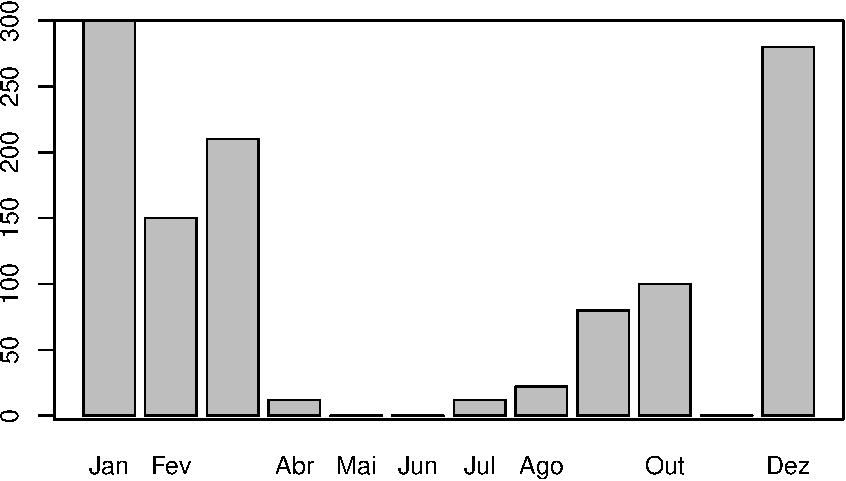
\includegraphics{images/chunk720-1.pdf}

\begin{Shaded}
\begin{Highlighting}[]
\CommentTok{# temperatura do ar média mensal para um dado ano}
\NormalTok{temp <-}\StringTok{ }\KeywordTok{c}\NormalTok{(}\DecValTok{25}\NormalTok{, }\FloatTok{23.2}\NormalTok{, }\FloatTok{22.5}\NormalTok{, }\DecValTok{21}\NormalTok{, }\DecValTok{19}\NormalTok{, }\FloatTok{17.6}\NormalTok{, }\DecValTok{18}\NormalTok{, }\FloatTok{19.7}\NormalTok{, }\FloatTok{21.3}\NormalTok{, }\DecValTok{22}\NormalTok{, }\DecValTok{24}\NormalTok{, }\FloatTok{26.8}\NormalTok{)}
\KeywordTok{names}\NormalTok{(temp) <-}\StringTok{ }\NormalTok{meses}
\NormalTok{temp}
\CommentTok{#>  Jan  Fev  Mar  Abr  Mai  Jun  Jul  Ago  Set  Out  Nov  Dez }
\CommentTok{#> 25.0 23.2 22.5 21.0 19.0 17.6 18.0 19.7 21.3 22.0 24.0 26.8}
\KeywordTok{plot}\NormalTok{(temp, }\DataTypeTok{type =} \StringTok{"o"}\NormalTok{)}
\end{Highlighting}
\end{Shaded}

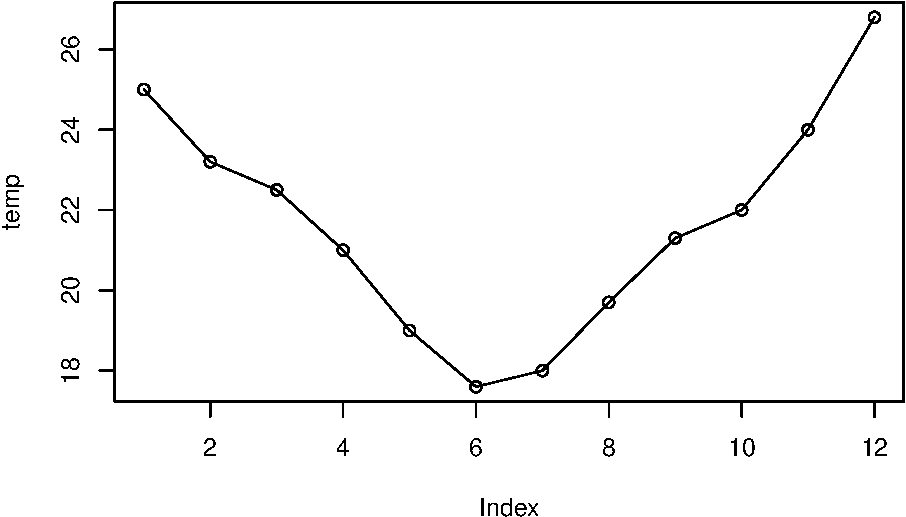
\includegraphics{images/chunk720-2.pdf}

Como selecionar o valor de chuva e temperatura só para janeiro?

Usando a seguinte sintaxe:

\texttt{vetor{[}i{]}}

onde \texttt{i} representa os elementos a serem selecionados.

\subsubsection{Indexação por vetores
inteiros}\label{indexacao-por-vetores-inteiros}

\paragraph{Positivos}\label{positivos}

Para selecionar o valor de chuva e temperatura só para janeiro,
digitamos:

\begin{Shaded}
\begin{Highlighting}[]
\NormalTok{prec_jan <-}\StringTok{ }\NormalTok{prec[}\DecValTok{1}\NormalTok{]}
\NormalTok{prec_jan}
\CommentTok{#> Jan }
\CommentTok{#> 300}
\NormalTok{temp_jan <-}\StringTok{ }\NormalTok{temp[}\DecValTok{1}\NormalTok{]}
\NormalTok{temp_jan}
\CommentTok{#> Jan }
\CommentTok{#>  25}
\end{Highlighting}
\end{Shaded}

Como selecionar os últimos valores dos vetores de chuva e temperatura?

\begin{Shaded}
\begin{Highlighting}[]
\CommentTok{# vetor de temperatura do ar média mensal de um ano qualquer}
\NormalTok{temp_dez <-}\StringTok{ }\NormalTok{temp[}\KeywordTok{length}\NormalTok{(temp)]}
\NormalTok{temp_dez}
\CommentTok{#>  Dez }
\CommentTok{#> 26.8}
\NormalTok{prec_dez <-}\StringTok{ }\NormalTok{prec[}\KeywordTok{length}\NormalTok{(prec)]}
\NormalTok{prec_dez}
\CommentTok{#> Dez }
\CommentTok{#> 280}
\end{Highlighting}
\end{Shaded}

Como selecionar os valores de chuva do trimestre JJA e de temperatura
para o trimestre DJF?

\begin{Shaded}
\begin{Highlighting}[]
\NormalTok{sel_prec <-}\StringTok{ }\KeywordTok{c}\NormalTok{(}\DecValTok{6}\NormalTok{, }\DecValTok{7}\NormalTok{, }\DecValTok{8}\NormalTok{)}
\CommentTok{# vetor de chuva JJA}
\NormalTok{prec_jja <-}\StringTok{ }\NormalTok{prec[sel_prec]}
\NormalTok{prec_jja}
\CommentTok{#> Jun Jul Ago }
\CommentTok{#>   0  12  22}
\CommentTok{# total de chuva trimestral nesse ano}
\NormalTok{prect_jja_tot <-}\StringTok{ }\KeywordTok{sum}\NormalTok{(prec_jja)}
\NormalTok{prect_jja_tot}
\CommentTok{#> [1] 34}
\CommentTok{# vetor de temperatura DJF}
\NormalTok{sel_temp <-}\StringTok{ }\KeywordTok{c}\NormalTok{(}\DecValTok{12}\NormalTok{, }\DecValTok{1}\NormalTok{, }\DecValTok{2}\NormalTok{)}
\NormalTok{temp_djf <-}\StringTok{ }\NormalTok{temp[sel_temp]}
\NormalTok{temp_djf}
\CommentTok{#>  Dez  Jan  Fev }
\CommentTok{#> 26.8 25.0 23.2}
\CommentTok{# temp média trimestral nesse ano}
\NormalTok{temp_djf_med <-}\StringTok{ }\KeywordTok{mean}\NormalTok{(temp_djf)}
\NormalTok{temp_djf_med}
\CommentTok{#> [1] 25}
\end{Highlighting}
\end{Shaded}

\paragraph{Negativos}\label{negativos}

Como selecionar todos valores menos o primeiro e o último?

\begin{Shaded}
\begin{Highlighting}[]
\CommentTok{# exceto o primeiro e ultimo}
\NormalTok{prec[}\OperatorTok{-}\KeywordTok{c}\NormalTok{(}\DecValTok{1}\NormalTok{, }\KeywordTok{length}\NormalTok{(prec))]}
\CommentTok{#> Fev Mar Abr Mai Jun Jul Ago Set Out Nov }
\CommentTok{#> 150 210  12   0   0  12  22  80 100   0}
\CommentTok{# exceto os 3 primeiros meses}
\NormalTok{temp[}\OperatorTok{-}\KeywordTok{c}\NormalTok{(}\DecValTok{1}\OperatorTok{:}\DecValTok{3}\NormalTok{)]}
\CommentTok{#>  Abr  Mai  Jun  Jul  Ago  Set  Out  Nov  Dez }
\CommentTok{#> 21.0 19.0 17.6 18.0 19.7 21.3 22.0 24.0 26.8}
\CommentTok{# exceto os 3 últimos meses}
\NormalTok{temp[}\OperatorTok{-}\KeywordTok{c}\NormalTok{(}\KeywordTok{length}\NormalTok{(temp)}\OperatorTok{:}\NormalTok{(}\KeywordTok{length}\NormalTok{(temp) }\OperatorTok{-}\StringTok{ }\DecValTok{2}\NormalTok{))]}
\CommentTok{#>  Jan  Fev  Mar  Abr  Mai  Jun  Jul  Ago  Set }
\CommentTok{#> 25.0 23.2 22.5 21.0 19.0 17.6 18.0 19.7 21.3}
\end{Highlighting}
\end{Shaded}

\subsubsection{Indexação por nomes}\label{indexacao-por-nomes}

\begin{Shaded}
\begin{Highlighting}[]
\NormalTok{prec[}\StringTok{"Jan"}\NormalTok{]}
\CommentTok{#> Jan }
\CommentTok{#> 300}
\NormalTok{prec[}\KeywordTok{c}\NormalTok{(}\StringTok{"Dez"}\NormalTok{, }\StringTok{"Fev"}\NormalTok{, }\StringTok{"Jun"}\NormalTok{)]}
\CommentTok{#> Dez Fev Jun }
\CommentTok{#> 280 150   0}
\end{Highlighting}
\end{Shaded}

\subsubsection{Indexação por vetores
lógicos}\label{indexacao-por-vetores-logicos}

Vamos criar um vetor lógico e usá-lo para exemplificar a seleção lógica
de elementos de um vetor.

\begin{Shaded}
\begin{Highlighting}[]
\NormalTok{vetor_l <-}\StringTok{ }\KeywordTok{c}\NormalTok{(}\OtherTok{TRUE}\NormalTok{, }\OtherTok{FALSE}\NormalTok{, }\OtherTok{FALSE}\NormalTok{, }\OtherTok{TRUE}\NormalTok{, }\OtherTok{TRUE}\NormalTok{, }\OtherTok{FALSE}\NormalTok{, }\OtherTok{TRUE}\NormalTok{, }\OtherTok{FALSE}\NormalTok{, }\OtherTok{TRUE}\NormalTok{, }\OtherTok{FALSE}\NormalTok{, }
    \OtherTok{FALSE}\NormalTok{, }\OtherTok{TRUE}\NormalTok{)}
\NormalTok{meses[vetor_l]}
\CommentTok{#> [1] "Jan" "Abr" "Mai" "Jul" "Set" "Dez"}
\end{Highlighting}
\end{Shaded}

Os elementos de \texttt{vetor\_l} correspondentes a \texttt{TRUE} foram
selecionados. Aplicando-se a função \texttt{sum()} a um vetor lógico
obtemos o total de elementos verdadeiros:

\begin{Shaded}
\begin{Highlighting}[]
\KeywordTok{sum}\NormalTok{(vetor_l)}
\CommentTok{#> [1] 6}
\end{Highlighting}
\end{Shaded}

Vamos considerar agora a seguinte forma do vetor lógico
(\texttt{vetor\_l}) e relembrar da \textbf{coerção} de vetores.

\begin{Shaded}
\begin{Highlighting}[]
\CommentTok{# vetor lógico}
\NormalTok{vetor_l <-}\StringTok{ }\KeywordTok{c}\NormalTok{(}\OtherTok{TRUE}\NormalTok{, }\OtherTok{FALSE}\NormalTok{)}
\NormalTok{meses[vetor_l]}
\CommentTok{#> [1] "Jan" "Mar" "Mai" "Jul" "Set" "Nov"}
\NormalTok{vetor_l <-}\StringTok{ }\KeywordTok{c}\NormalTok{(}\OtherTok{TRUE}\NormalTok{, }\OtherTok{FALSE}\NormalTok{, }\OtherTok{FALSE}\NormalTok{)}
\NormalTok{meses[vetor_l]}
\CommentTok{#> [1] "Jan" "Abr" "Jul" "Out"}
\NormalTok{prec[}\KeywordTok{c}\NormalTok{(}\OtherTok{TRUE}\NormalTok{, }\OtherTok{FALSE}\NormalTok{)]}
\CommentTok{#> Jan Mar Mai Jul Set Nov }
\CommentTok{#> 300 210   0  12  80   0}
\NormalTok{temp[}\KeywordTok{c}\NormalTok{(}\KeywordTok{rep}\NormalTok{(}\OtherTok{FALSE}\NormalTok{, }\DecValTok{3}\NormalTok{), }\OtherTok{TRUE}\NormalTok{)]}
\CommentTok{#>  Abr  Ago  Dez }
\CommentTok{#> 21.0 19.7 26.8}
\end{Highlighting}
\end{Shaded}

A indexação pode ser feita também por comparações:

\begin{Shaded}
\begin{Highlighting}[]
\CommentTok{# vetor prec}
\NormalTok{prec}
\CommentTok{#> Jan Fev Mar Abr Mai Jun Jul Ago Set Out Nov Dez }
\CommentTok{#> 300 150 210  12   0   0  12  22  80 100   0 280}
\CommentTok{# teste para chuva > 80 mm/mês}
\NormalTok{prec }\OperatorTok{>}\StringTok{ }\DecValTok{80}
\CommentTok{#>   Jan   Fev   Mar   Abr   Mai   Jun   Jul   Ago   Set   Out   Nov   Dez }
\CommentTok{#>  TRUE  TRUE  TRUE FALSE FALSE FALSE FALSE FALSE FALSE  TRUE FALSE  TRUE}
\CommentTok{# salvando resultado do teste}
\NormalTok{above80 <-}\StringTok{ }\NormalTok{prec }\OperatorTok{>}\StringTok{ }\DecValTok{80}
\CommentTok{# extraindo valores atendidos ao teste}
\NormalTok{prec[above80]}
\CommentTok{#> Jan Fev Mar Out Dez }
\CommentTok{#> 300 150 210 100 280}
\CommentTok{# teste para meses com chuva abaixo da média mensal}
\NormalTok{(prec_med <-}\StringTok{ }\KeywordTok{mean}\NormalTok{(prec))}
\CommentTok{#> [1] 97.1667}
\CommentTok{# salvando resultado do teste}
\NormalTok{(below_avg <-}\StringTok{ }\NormalTok{prec }\OperatorTok{<}\StringTok{ }\NormalTok{prec_med)}
\CommentTok{#>   Jan   Fev   Mar   Abr   Mai   Jun   Jul   Ago   Set   Out   Nov   Dez }
\CommentTok{#> FALSE FALSE FALSE  TRUE  TRUE  TRUE  TRUE  TRUE  TRUE FALSE  TRUE FALSE}
\CommentTok{# extraindo valores que atendem a condição}
\NormalTok{prec[below_avg]}
\CommentTok{#> Abr Mai Jun Jul Ago Set Nov }
\CommentTok{#>  12   0   0  12  22  80   0}
\CommentTok{# extraindo os 3 primeiros meses com prec abaixo da média}
\NormalTok{prec[below_avg][}\DecValTok{1}\OperatorTok{:}\DecValTok{3}\NormalTok{]}
\CommentTok{#> Abr Mai Jun }
\CommentTok{#>  12   0   0}
\CommentTok{# forma equivalente em uma linha só}
\NormalTok{prec[prec }\OperatorTok{<}\StringTok{ }\KeywordTok{mean}\NormalTok{(prec)][}\DecValTok{1}\OperatorTok{:}\DecValTok{3}\NormalTok{]}
\CommentTok{#> Abr Mai Jun }
\CommentTok{#>  12   0   0}
\CommentTok{# teste para meses com prec diferente de zero}
\NormalTok{prec[prec }\OperatorTok{!=}\StringTok{ }\DecValTok{0}\NormalTok{]}
\CommentTok{#> Jan Fev Mar Abr Jul Ago Set Out Dez }
\CommentTok{#> 300 150 210  12  12  22  80 100 280}
\end{Highlighting}
\end{Shaded}

\subsubsection{Indexação com múltiplas
condições}\label{indexacao-com-multiplas-condicoes}

Nos exemplo acima vimos como buscar os os elementos de um vetor para
apenas uma condição. Entretanto frequentemente precisamos testar mais
condições. Por exemplo, para condições do tipo:

\begin{itemize}
\tightlist
\item
  \(0.5 < prec \leq 100\)
\item
  \(temp < 5\) ou \(temp \geq 25\)
\end{itemize}

precisamos usar os operadores relacionais:

\begin{itemize}
\item
  \texttt{\&} e \texttt{\&\&} ("e``)
\item
  \texttt{\textbar{}} e \texttt{\textbar{}\textbar{}} ("ou``)
\end{itemize}

A ordem das operações pode ser controladas por parênteses. Os operadores
\texttt{\&} e \texttt{\textbar{}} são vetorizados (retornam vetores de
mesmo tamanho que os vetores testados).

As diferenças entre os operadores são mostradas nos exemplos a seguir.

\begin{Shaded}
\begin{Highlighting}[]
\CommentTok{# prec}
\NormalTok{prec}
\CommentTok{#> Jan Fev Mar Abr Mai Jun Jul Ago Set Out Nov Dez }
\CommentTok{#> 300 150 210  12   0   0  12  22  80 100   0 280}
\CommentTok{# combinação de operador lógico e relacional}
\NormalTok{below100 <-}\StringTok{ }\NormalTok{prec }\OperatorTok{>}\StringTok{ }\DecValTok{0} \OperatorTok{&}\StringTok{ }\NormalTok{prec }\OperatorTok{<=}\StringTok{ }\DecValTok{100}
\NormalTok{prec_cond1 <-}\StringTok{ }\NormalTok{prec[below100]}
\NormalTok{prec_cond1}
\CommentTok{#> Abr Jul Ago Set Out }
\CommentTok{#>  12  12  22  80 100}
\end{Highlighting}
\end{Shaded}

A forma dupla (\texttt{\&\&} ou \texttt{\textbar{}\textbar{}}) compara
somente um elemento de cada lado, enquanto a forma normal (\texttt{\&} e
\texttt{\textbar{}}), compara cada elemento dos vetores em cada lado.

\begin{Shaded}
\begin{Highlighting}[]
\NormalTok{a <-}\StringTok{ }\KeywordTok{c}\NormalTok{(}\DecValTok{1}\NormalTok{, }\DecValTok{1}\NormalTok{, }\DecValTok{0}\NormalTok{, }\DecValTok{1}\NormalTok{)}
\NormalTok{b <-}\StringTok{ }\KeywordTok{c}\NormalTok{(}\DecValTok{2}\NormalTok{, }\DecValTok{1}\NormalTok{, }\DecValTok{0}\NormalTok{, }\DecValTok{1}\NormalTok{)}
\CommentTok{# forma normal verifica cada elemento de a e cada elemento de b}
\NormalTok{a }\OperatorTok{==}\StringTok{ }\DecValTok{1} \OperatorTok{&}\StringTok{ }\NormalTok{b }\OperatorTok{==}\StringTok{ }\DecValTok{1}
\CommentTok{#> [1] FALSE  TRUE FALSE  TRUE}
\CommentTok{# forma dupla verifica somente o primeiro elemento de a e o primeiro}
\CommentTok{# elemento de b retornando somente um resultado}
\NormalTok{a }\OperatorTok{==}\StringTok{ }\DecValTok{1} \OperatorTok{&&}\StringTok{ }\NormalTok{b }\OperatorTok{==}\StringTok{ }\DecValTok{1}
\CommentTok{#> [1] FALSE}
\end{Highlighting}
\end{Shaded}

\begin{longtable}[]{@{}cccccc@{}}
\caption{Demostração da diferença entre \& e \&\&.}\tabularnewline
\toprule
\begin{minipage}[b]{0.05\columnwidth}\centering\strut
a\strut
\end{minipage} & \begin{minipage}[b]{0.05\columnwidth}\centering\strut
b\strut
\end{minipage} & \begin{minipage}[b]{0.09\columnwidth}\centering\strut
a==1\strut
\end{minipage} & \begin{minipage}[b]{0.09\columnwidth}\centering\strut
b==1\strut
\end{minipage} & \begin{minipage}[b]{0.21\columnwidth}\centering\strut
a == 1 \& b == 1\strut
\end{minipage} & \begin{minipage}[b]{0.21\columnwidth}\centering\strut
a == 1 \&\& b == 1\strut
\end{minipage}\tabularnewline
\midrule
\endfirsthead
\toprule
\begin{minipage}[b]{0.05\columnwidth}\centering\strut
a\strut
\end{minipage} & \begin{minipage}[b]{0.05\columnwidth}\centering\strut
b\strut
\end{minipage} & \begin{minipage}[b]{0.09\columnwidth}\centering\strut
a==1\strut
\end{minipage} & \begin{minipage}[b]{0.09\columnwidth}\centering\strut
b==1\strut
\end{minipage} & \begin{minipage}[b]{0.21\columnwidth}\centering\strut
a == 1 \& b == 1\strut
\end{minipage} & \begin{minipage}[b]{0.21\columnwidth}\centering\strut
a == 1 \&\& b == 1\strut
\end{minipage}\tabularnewline
\midrule
\endhead
\begin{minipage}[t]{0.05\columnwidth}\centering\strut
1\strut
\end{minipage} & \begin{minipage}[t]{0.05\columnwidth}\centering\strut
2\strut
\end{minipage} & \begin{minipage}[t]{0.09\columnwidth}\centering\strut
TRUE\strut
\end{minipage} & \begin{minipage}[t]{0.09\columnwidth}\centering\strut
FALSE\strut
\end{minipage} & \begin{minipage}[t]{0.21\columnwidth}\centering\strut
FALSE\strut
\end{minipage} & \begin{minipage}[t]{0.21\columnwidth}\centering\strut
FALSE\strut
\end{minipage}\tabularnewline
\begin{minipage}[t]{0.05\columnwidth}\centering\strut
1\strut
\end{minipage} & \begin{minipage}[t]{0.05\columnwidth}\centering\strut
1\strut
\end{minipage} & \begin{minipage}[t]{0.09\columnwidth}\centering\strut
TRUE\strut
\end{minipage} & \begin{minipage}[t]{0.09\columnwidth}\centering\strut
TRUE\strut
\end{minipage} & \begin{minipage}[t]{0.21\columnwidth}\centering\strut
TRUE\strut
\end{minipage} & \begin{minipage}[t]{0.21\columnwidth}\centering\strut
\strut
\end{minipage}\tabularnewline
\begin{minipage}[t]{0.05\columnwidth}\centering\strut
0\strut
\end{minipage} & \begin{minipage}[t]{0.05\columnwidth}\centering\strut
0\strut
\end{minipage} & \begin{minipage}[t]{0.09\columnwidth}\centering\strut
FALSE\strut
\end{minipage} & \begin{minipage}[t]{0.09\columnwidth}\centering\strut
FALSE\strut
\end{minipage} & \begin{minipage}[t]{0.21\columnwidth}\centering\strut
FALSE\strut
\end{minipage} & \begin{minipage}[t]{0.21\columnwidth}\centering\strut
\strut
\end{minipage}\tabularnewline
\begin{minipage}[t]{0.05\columnwidth}\centering\strut
1\strut
\end{minipage} & \begin{minipage}[t]{0.05\columnwidth}\centering\strut
1\strut
\end{minipage} & \begin{minipage}[t]{0.09\columnwidth}\centering\strut
TRUE\strut
\end{minipage} & \begin{minipage}[t]{0.09\columnwidth}\centering\strut
TRUE\strut
\end{minipage} & \begin{minipage}[t]{0.21\columnwidth}\centering\strut
TRUE\strut
\end{minipage} & \begin{minipage}[t]{0.21\columnwidth}\centering\strut
\strut
\end{minipage}\tabularnewline
\bottomrule
\end{longtable}

Podem haver mais que duas condições a serem testadas. As condições podem
ser combinadas usando múltiplos \texttt{\&} ou \texttt{\textbar{}}. As
diferentes condições podem ser agrupadas por parênteses assim como
operações matemáticas. Sem parênteses, a ordem das operações é
semelhante a das operações matemáticas:

\begin{itemize}
\tightlist
\item
  \textbf{PEMDAS}: Parênteses \textgreater{} Expoentes \textgreater{}
  Multiplicação \textgreater{} Divisão \textgreater{} Adição e Subtração
\end{itemize}

Onde \texttt{\&}é equivalente à \textbf{multiplicação} e
\texttt{\textbar{}} é equivalente à \textbf{adição}, logo \textbf{e} tem
precedência sobre \textbf{ou}.

\begin{Shaded}
\begin{Highlighting}[]
\CommentTok{# vetor de horas}
\NormalTok{horas <-}\StringTok{ }\DecValTok{0}\OperatorTok{:}\DecValTok{23}
\CommentTok{# vetor de temperaturas horárias}
\NormalTok{tar_hor <-}\StringTok{ }\KeywordTok{c}\NormalTok{(}
  \FloatTok{19.9}\NormalTok{, }\FloatTok{19.8}\NormalTok{, }\FloatTok{19.5}\NormalTok{, }\FloatTok{19.4}\NormalTok{, }\FloatTok{19.4}\NormalTok{, }\FloatTok{19.3}\NormalTok{,}
  \FloatTok{19.2}\NormalTok{, }\DecValTok{19}\NormalTok{, }\FloatTok{19.2}\NormalTok{, }\FloatTok{19.5}\NormalTok{, }\FloatTok{20.1}\NormalTok{, }\FloatTok{20.6}\NormalTok{, }\FloatTok{20.9}\NormalTok{,}
  \FloatTok{21.8}\NormalTok{, }\FloatTok{22.5}\NormalTok{, }\FloatTok{22.6}\NormalTok{, }\FloatTok{22.5}\NormalTok{, }\DecValTok{22}\NormalTok{, }\FloatTok{21.4}\NormalTok{, }\FloatTok{20.1}\NormalTok{,}
  \DecValTok{20}\NormalTok{, }\FloatTok{19.8}\NormalTok{, }\FloatTok{19.6}\NormalTok{, }\FloatTok{19.4}
\NormalTok{)}
\CommentTok{# gráfico do varição horária da temperatura do ar}
\KeywordTok{plot}\NormalTok{(horas, tar_hor, }\DataTypeTok{type =} \StringTok{"o"}\NormalTok{, }\DataTypeTok{pch =} \DecValTok{20}\NormalTok{)}
\CommentTok{# temperaturas noturnas abaixo de 20ºC}
\NormalTok{(night_below20 <-}\StringTok{ }\NormalTok{(horas }\OperatorTok{<}\StringTok{ }\DecValTok{6} \OperatorTok{|}\StringTok{ }\NormalTok{horas }\OperatorTok{>}\StringTok{ }\DecValTok{18}\NormalTok{) }\OperatorTok{&}\StringTok{ }\NormalTok{tar_hor }\OperatorTok{<}\StringTok{ }\DecValTok{20}\NormalTok{)}
\CommentTok{#>  [1]  TRUE  TRUE  TRUE  TRUE  TRUE  TRUE FALSE FALSE FALSE FALSE FALSE}
\CommentTok{#> [12] FALSE FALSE FALSE FALSE FALSE FALSE FALSE FALSE FALSE FALSE  TRUE}
\CommentTok{#> [23]  TRUE  TRUE}
\NormalTok{tar_hor[night_below20]}
\CommentTok{#> [1] 19.9 19.8 19.5 19.4 19.4 19.3 19.8 19.6 19.4}
\CommentTok{# destacando no gráfico}
\KeywordTok{points}\NormalTok{(}
  \DataTypeTok{x =}\NormalTok{ horas[night_below20],}
  \DataTypeTok{y =}\NormalTok{ tar_hor[night_below20],}
  \DataTypeTok{pch =} \DecValTok{20}\NormalTok{, }\CommentTok{# tipo de símbolo para os ponts}
  \DataTypeTok{col =} \StringTok{"blue"}\NormalTok{, }\CommentTok{# cor do símbolo}
  \DataTypeTok{cex =} \DecValTok{2}
\NormalTok{) }\CommentTok{# tamanho do ponto}
\CommentTok{# temperaturas abaixo de 20ºC que não ocorreram a noite}
\NormalTok{day_below20 <-}\StringTok{ }\NormalTok{tar_hor }\OperatorTok{<}\StringTok{ }\DecValTok{20} \OperatorTok{&}\StringTok{ }\OperatorTok{!}\NormalTok{night_below20}
\KeywordTok{points}\NormalTok{(horas[day_below20], tar_hor[day_below20], }\DataTypeTok{pch =} \DecValTok{20}\NormalTok{, }\DataTypeTok{col =} \StringTok{"red"}\NormalTok{, }\DataTypeTok{cex =} \DecValTok{2}\NormalTok{)}
\CommentTok{# adicionando linha horizontal ao longo da temperatura = 20ºC}
\KeywordTok{abline}\NormalTok{(}\DataTypeTok{h =} \DecValTok{20}\NormalTok{, }\DataTypeTok{col =} \StringTok{"gray"}\NormalTok{)}
\end{Highlighting}
\end{Shaded}

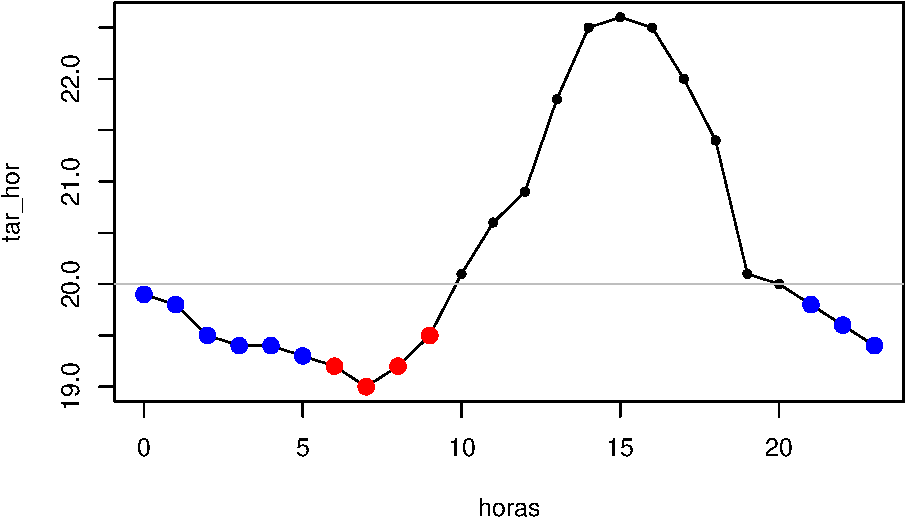
\includegraphics{images/chunk7292-1.pdf}

Vimos que a filtragem consiste em extrair elementos de um vetor que
satisfaça uma (ou várias) condição(ões). Entretanto, em alguns casos, o
interesse é na posição dentro do vetor na qual a condição é verdadeira
Nós podemos localizar essas ocorrências usando a função
\texttt{which()}:

\begin{Shaded}
\begin{Highlighting}[]
\CommentTok{# prec sem nomes}
\KeywordTok{names}\NormalTok{(prec) <-}\StringTok{ }\OtherTok{NULL}
\CommentTok{# combinação de operador lógico e relacional}
\NormalTok{below100}
\CommentTok{#>   Jan   Fev   Mar   Abr   Mai   Jun   Jul   Ago   Set   Out   Nov   Dez }
\CommentTok{#> FALSE FALSE FALSE  TRUE FALSE FALSE  TRUE  TRUE  TRUE  TRUE FALSE FALSE}
\KeywordTok{which}\NormalTok{(below100)}
\CommentTok{#> Abr Jul Ago Set Out }
\CommentTok{#>   4   7   8   9  10}
\CommentTok{# qual os meses em que a chuva foi acima da media}
\KeywordTok{which}\NormalTok{(prec }\OperatorTok{>}\StringTok{ }\NormalTok{prec_med)}
\CommentTok{#> [1]  1  2  3 10 12}
\NormalTok{prec[}\KeywordTok{which}\NormalTok{(prec }\OperatorTok{>}\StringTok{ }\NormalTok{prec_med)]}
\CommentTok{#> [1] 300 150 210 100 280}
\CommentTok{# Qual a temp quando a chuva ou a temp foi acima da media?}
\NormalTok{sel <-}\StringTok{ }\KeywordTok{which}\NormalTok{(prec }\OperatorTok{>}\StringTok{ }\NormalTok{prec_med }\OperatorTok{|}\StringTok{ }\OperatorTok{!}\NormalTok{temp }\OperatorTok{<}\StringTok{ }\KeywordTok{mean}\NormalTok{(temp))}
\NormalTok{sel}
\CommentTok{#> Jan Fev Mar Out Nov Dez }
\CommentTok{#>   1   2   3  10  11  12}
\NormalTok{prec[sel]}
\CommentTok{#> [1] 300 150 210 100   0 280}
\CommentTok{# quais posições do vetor prec não choveu}
\KeywordTok{which}\NormalTok{(prec }\OperatorTok{==}\StringTok{ }\DecValTok{0}\NormalTok{)}
\CommentTok{#> [1]  5  6 11}
\CommentTok{# quando ocorreu a prec max}
\KeywordTok{which}\NormalTok{(prec }\OperatorTok{==}\StringTok{ }\KeywordTok{max}\NormalTok{(prec))}
\CommentTok{#> [1] 1}
\CommentTok{# equivalente a ...}
\KeywordTok{which.max}\NormalTok{(prec)}
\CommentTok{#> [1] 1}
\CommentTok{# seleciona só a primeira ocorrência!}
\KeywordTok{which.min}\NormalTok{(prec)}
\CommentTok{#> [1] 5}
\NormalTok{prec}
\CommentTok{#>  [1] 300 150 210  12   0   0  12  22  80 100   0 280}
\end{Highlighting}
\end{Shaded}

Um outro operador útil para comparação entre vetores é o operador
\texttt{\%in\%}, que pode ser interpretado como "está contido em". O
\textbf{resultado é um vetor de mesmo tamanho que o vetor à esquerda do
teste}.

\begin{Shaded}
\begin{Highlighting}[]
\CommentTok{# compare o tamanho dos vetores resultantes}
\KeywordTok{which}\NormalTok{(meses }\OperatorTok\StringTok{ }\KeywordTok{c}\NormalTok{(}\StringTok{"JAN"}\NormalTok{, }\StringTok{"Feb"}\NormalTok{, }\StringTok{"Mar"}\NormalTok{))}
\CommentTok{#> [1] 3}
\CommentTok{# note a diferença}
\KeywordTok{which}\NormalTok{(}\KeywordTok{c}\NormalTok{(}\StringTok{"JAN"}\NormalTok{, }\StringTok{"Feb"}\NormalTok{, }\StringTok{"Mar"}\NormalTok{) }\OperatorTok\StringTok{ }\NormalTok{meses)}
\CommentTok{#> [1] 3}
\NormalTok{cond <-}\StringTok{ }\KeywordTok{names}\NormalTok{(temp) }\OperatorTok\StringTok{ }\KeywordTok{c}\NormalTok{(}\StringTok{"Jun"}\NormalTok{, }\StringTok{"Jul"}\NormalTok{, }\StringTok{"Ago"}\NormalTok{)}
\NormalTok{quais <-}\StringTok{ }\KeywordTok{which}\NormalTok{(cond)}
\NormalTok{quais}
\CommentTok{#> [1] 6 7 8}
\NormalTok{prec[cond]}
\CommentTok{#> [1]  0 12 22}
\NormalTok{prec[quais]}
\CommentTok{#> [1]  0 12 22}
\end{Highlighting}
\end{Shaded}

\subsection{Substituição de elementos de um
vetor}\label{substituicao-de-elementos-de-um-vetor}

\begin{Shaded}
\begin{Highlighting}[]
\CommentTok{# posição a ser alterada}
\NormalTok{pos <-}\StringTok{ }\DecValTok{10}
\CommentTok{# valor da temperatura naquela posição}
\NormalTok{old_temp <-}\StringTok{ }\NormalTok{temp[pos]}
\NormalTok{old_temp}
\CommentTok{#> Out }
\CommentTok{#>  22}
\CommentTok{# vetor de temperatura}
\NormalTok{temp}
\CommentTok{#>  Jan  Fev  Mar  Abr  Mai  Jun  Jul  Ago  Set  Out  Nov  Dez }
\CommentTok{#> 25.0 23.2 22.5 21.0 19.0 17.6 18.0 19.7 21.3 22.0 24.0 26.8}
\CommentTok{# substituição do valor original por um novo valor}
\NormalTok{new_temp <-}\StringTok{ }\DecValTok{30}
\CommentTok{# alterando temperatura do mês de outubro}
\NormalTok{temp[pos] <-}\StringTok{ }\NormalTok{new_temp}
\NormalTok{temp}
\CommentTok{#>  Jan  Fev  Mar  Abr  Mai  Jun  Jul  Ago  Set  Out  Nov  Dez }
\CommentTok{#> 25.0 23.2 22.5 21.0 19.0 17.6 18.0 19.7 21.3 30.0 24.0 26.8}
\end{Highlighting}
\end{Shaded}

A substituição também pode ser feita também pelo nome das variáveis.

\begin{Shaded}
\begin{Highlighting}[]
\NormalTok{prec}
\CommentTok{#>  [1] 300 150 210  12   0   0  12  22  80 100   0 280}
\NormalTok{prec[}\StringTok{"Mai"}\NormalTok{] <-}\StringTok{ }\DecValTok{5}
\NormalTok{temp}
\CommentTok{#>  Jan  Fev  Mar  Abr  Mai  Jun  Jul  Ago  Set  Out  Nov  Dez }
\CommentTok{#> 25.0 23.2 22.5 21.0 19.0 17.6 18.0 19.7 21.3 30.0 24.0 26.8}
\NormalTok{temp[}\KeywordTok{c}\NormalTok{(}\StringTok{"Mai"}\NormalTok{, }\StringTok{"Jul"}\NormalTok{)] <-}\StringTok{ }\NormalTok{temp[}\KeywordTok{c}\NormalTok{(}\StringTok{"Mai"}\NormalTok{, }\StringTok{"Jul"}\NormalTok{)] }\OperatorTok{+}\StringTok{ }\DecValTok{2}
\NormalTok{temp}
\CommentTok{#>  Jan  Fev  Mar  Abr  Mai  Jun  Jul  Ago  Set  Out  Nov  Dez }
\CommentTok{#> 25.0 23.2 22.5 21.0 21.0 17.6 20.0 19.7 21.3 30.0 24.0 26.8}
\end{Highlighting}
\end{Shaded}

\subsection{\texorpdfstring{Criação de vetores com
\texttt{vector}}{Criação de vetores com vector}}\label{criacao-de-vetores-com-vector}

Outra forma de se criar vetores é através da função \texttt{vector()}.

\begin{Shaded}
\begin{Highlighting}[]
\CommentTok{# criação de vetor v}
\NormalTok{v <-}\StringTok{ }\DecValTok{3}
\NormalTok{v}
\CommentTok{#> [1] 3}
\CommentTok{# adicionando elementos}
\NormalTok{v[}\DecValTok{2}\NormalTok{] <-}\StringTok{ }\DecValTok{100}
\NormalTok{v}
\CommentTok{#> [1]   3 100}
\NormalTok{v[}\DecValTok{5}\NormalTok{] <-}\StringTok{ }\DecValTok{6}
\NormalTok{v}
\CommentTok{#> [1]   3 100  NA  NA   6}
\CommentTok{# adicionando elementos de vetores}
\NormalTok{x <-}\StringTok{ }\KeywordTok{c}\NormalTok{(}\DecValTok{88}\NormalTok{, }\DecValTok{5}\NormalTok{, }\DecValTok{12}\NormalTok{, }\DecValTok{13}\NormalTok{)}
\NormalTok{x <-}\StringTok{ }\KeywordTok{c}\NormalTok{(x[}\DecValTok{1}\OperatorTok{:}\DecValTok{3}\NormalTok{], }\DecValTok{168}\NormalTok{, x[}\DecValTok{4}\NormalTok{])  }\CommentTok{# insere 168 antes do 13}
\NormalTok{x}
\CommentTok{#> [1]  88   5  12 168  13}
\CommentTok{# outra opção}
\NormalTok{k <-}\StringTok{ }\KeywordTok{vector}\NormalTok{()}
\KeywordTok{class}\NormalTok{(k)}
\CommentTok{#> [1] "logical"}
\CommentTok{# vetor k existe?}
\KeywordTok{ls}\NormalTok{()}
\CommentTok{#>  [1] "a"             "above80"       "an"            "anos"         }
\CommentTok{#>  [5] "anos_dec"      "a_sn"          "b"             "below100"     }
\CommentTok{#>  [9] "below_avg"     "chuva"         "cond"          "cte"          }
\CommentTok{#> [13] "day_below20"   "dda"           "decd"          "desc"         }
\CommentTok{#> [17] "frac_d30mn"    "horas"         "k"             "meses"        }
\CommentTok{#> [21] "months"        "new_temp"      "night_below20" "old_temp"     }
\CommentTok{#> [25] "oper"          "pcks"          "pent"          "pos"          }
\CommentTok{#> [29] "prec"          "prec_cond1"    "prec_dez"      "prec_jan"     }
\CommentTok{#> [33] "prec_jja"      "prec_med"      "prect_jja_tot" "quais"        }
\CommentTok{#> [37] "rblue"         "rep_e31"       "rep_t13"       "rep_t13_t4"   }
\CommentTok{#> [41] "rep_t4"        "s5by"          "s5len"         "seco"         }
\CommentTok{#> [45] "seco01"        "sel"           "sel_prec"      "sel_temp"     }
\CommentTok{#> [49] "seqn"          "si_dec"        "snum_b"        "tar_hor"      }
\CommentTok{#> [53] "temp"          "temp_dez"      "temp_djf"      "temp_djf_med" }
\CommentTok{#> [57] "temp_jan"      "v"             "v1"            "v_123"        }
\CommentTok{#> [61] "v_123a"        "v_123b"        "v2"            "v3"           }
\CommentTok{#> [65] "vetor"         "vetor_char"    "vetor_int"     "vetor_l"      }
\CommentTok{#> [69] "vetor_log"     "vetor_num"     "x"             "y"            }
\CommentTok{#> [73] "z"}
\CommentTok{# alocando o valor 45 no 3º elemento de k}
\NormalTok{k[}\DecValTok{3}\NormalTok{] <-}\StringTok{ }\DecValTok{45}
\NormalTok{k}
\CommentTok{#> [1] NA NA 45}
\KeywordTok{class}\NormalTok{(k)}
\CommentTok{#> [1] "numeric"}
\CommentTok{# diminuindo o tamanho de k}
\KeywordTok{length}\NormalTok{(k)}
\CommentTok{#> [1] 3}
\KeywordTok{length}\NormalTok{(k) <-}\StringTok{ }\DecValTok{2}
\NormalTok{k}
\CommentTok{#> [1] NA NA}
\KeywordTok{length}\NormalTok{(k) <-}\StringTok{ }\DecValTok{0}
\NormalTok{k}
\CommentTok{#> numeric(0)}
\KeywordTok{class}\NormalTok{(k)}
\CommentTok{#> [1] "numeric"}
\KeywordTok{is.null}\NormalTok{(k)}
\CommentTok{#> [1] FALSE}
\CommentTok{# exemplo}
\NormalTok{temp <-}\StringTok{ }\KeywordTok{c}\NormalTok{(}\DecValTok{25}\NormalTok{, }\FloatTok{23.2}\NormalTok{, }\FloatTok{22.5}\NormalTok{, }\DecValTok{21}\NormalTok{, }\DecValTok{19}\NormalTok{, }\FloatTok{17.6}\NormalTok{, }\DecValTok{18}\NormalTok{, }\FloatTok{19.7}\NormalTok{, }\FloatTok{21.3}\NormalTok{, }\DecValTok{22}\NormalTok{, }\DecValTok{24}\NormalTok{, }\FloatTok{26.8}\NormalTok{)}
\NormalTok{temp_orig <-}\StringTok{ }\NormalTok{temp}
\CommentTok{# mostrando o vetor temp}
\NormalTok{temp}
\CommentTok{#>  [1] 25.0 23.2 22.5 21.0 19.0 17.6 18.0 19.7 21.3 22.0 24.0 26.8}
\NormalTok{temp[]}
\CommentTok{#>  [1] 25.0 23.2 22.5 21.0 19.0 17.6 18.0 19.7 21.3 22.0 24.0 26.8}
\CommentTok{# substituir todos elementos do vetor temp por um vetor com apenas um valor}
\NormalTok{temp <-}\StringTok{ }\DecValTok{0}
\NormalTok{temp}
\CommentTok{#> [1] 0}
\CommentTok{# vamos redefinir temp e comparar o anterior com o obtido com o próximo}
\CommentTok{# comando}
\NormalTok{temp <-}\StringTok{ }\NormalTok{temp_orig}
\NormalTok{temp[}\DecValTok{1}\OperatorTok{:}\KeywordTok{length}\NormalTok{(temp)] <-}\StringTok{ }\DecValTok{0}
\NormalTok{temp}
\CommentTok{#>  [1] 0 0 0 0 0 0 0 0 0 0 0 0}
\CommentTok{# qual diferença de x <- 0 e x[] <-0 ?}
\NormalTok{temp <-}\StringTok{ }\NormalTok{temp_orig}
\NormalTok{temp[] <-}\StringTok{ }\DecValTok{0}
\NormalTok{temp}
\CommentTok{#>  [1] 0 0 0 0 0 0 0 0 0 0 0 0}
\CommentTok{# Um vetor com tamanho pre-definido e do tipo numeric}
\NormalTok{umvetor <-}\StringTok{ }\KeywordTok{vector}\NormalTok{(}\DataTypeTok{mode =} \StringTok{"numeric"}\NormalTok{, }\DataTypeTok{length =} \DecValTok{100}\NormalTok{)}
\NormalTok{umvetor}
\CommentTok{#>   [1] 0 0 0 0 0 0 0 0 0 0 0 0 0 0 0 0 0 0 0 0 0 0 0 0 0 0 0 0 0 0 0 0 0 0 0}
\CommentTok{#>  [36] 0 0 0 0 0 0 0 0 0 0 0 0 0 0 0 0 0 0 0 0 0 0 0 0 0 0 0 0 0 0 0 0 0 0 0}
\CommentTok{#>  [71] 0 0 0 0 0 0 0 0 0 0 0 0 0 0 0 0 0 0 0 0 0 0 0 0 0 0 0 0 0 0}
\CommentTok{# populando o vetor}
\NormalTok{umvetor[}\DecValTok{1}\NormalTok{] <-}\StringTok{ }\DecValTok{10}
\NormalTok{umvetor[}\DecValTok{10}\NormalTok{] <-}\StringTok{ }\DecValTok{100}
\NormalTok{umvetor}
\CommentTok{#>   [1]  10   0   0   0   0   0   0   0   0 100   0   0   0   0   0   0   0}
\CommentTok{#>  [18]   0   0   0   0   0   0   0   0   0   0   0   0   0   0   0   0   0}
\CommentTok{#>  [35]   0   0   0   0   0   0   0   0   0   0   0   0   0   0   0   0   0}
\CommentTok{#>  [52]   0   0   0   0   0   0   0   0   0   0   0   0   0   0   0   0   0}
\CommentTok{#>  [69]   0   0   0   0   0   0   0   0   0   0   0   0   0   0   0   0   0}
\CommentTok{#>  [86]   0   0   0   0   0   0   0   0   0   0   0   0   0   0   0}
\end{Highlighting}
\end{Shaded}

\subsection{Vetores nulos e elementos
faltantes}\label{vetores-nulos-e-elementos-faltantes}

Seja qual for a razão, ao realizar um experimento em condições reais
sempre haverá situações em que não conhecemos o valor de uma determinada
variável. Por exemplo, a série de uma variável meteorológica medida em
estação de superfície, sempre ocorrem datas em que não há registro da
variável. Falha instrumental, dado não coletado pelo observador, falta
de energia, são causas inerentes de falhas em séries climáticas de longo
prazo. No R dados faltantes são representados pela string \texttt{NA}.

\begin{Shaded}
\begin{Highlighting}[]
\NormalTok{v1 <-}\StringTok{ }\KeywordTok{c}\NormalTok{(}\DecValTok{1}\OperatorTok{:}\DecValTok{8}\NormalTok{, }\OtherTok{NA}\NormalTok{)}
\NormalTok{v1 }\OperatorTok{>}\StringTok{ }\DecValTok{5} \CommentTok{# NA sai na resposta}
\CommentTok{#> [1] FALSE FALSE FALSE FALSE FALSE  TRUE  TRUE  TRUE    NA}
\CommentTok{# teste lógico com o operador idêntico "=="}
\NormalTok{v1 }\OperatorTok{==}\StringTok{ }\OtherTok{NA}
\CommentTok{#> [1] NA NA NA NA NA NA NA NA NA}
\CommentTok{# não funcionou, porque há funções específicas para vetores com NA}
\NormalTok{onde_falta <-}\StringTok{ }\KeywordTok{is.na}\NormalTok{(v1)}
\CommentTok{# função apropriada p/ checar se tem NAs}
\NormalTok{faltante <-}\StringTok{ }\KeywordTok{which}\NormalTok{(}\KeywordTok{is.na}\NormalTok{(v1))}
\NormalTok{v1[}\OperatorTok{-}\NormalTok{faltante]}
\CommentTok{#> [1] 1 2 3 4 5 6 7 8}
\CommentTok{# ou}
\NormalTok{v1[}\OperatorTok{!}\NormalTok{onde_falta]}
\CommentTok{#> [1] 1 2 3 4 5 6 7 8}
\CommentTok{# vamos calcular a média de v1}
\KeywordTok{sum}\NormalTok{(v1) }\OperatorTok{/}\StringTok{ }\KeywordTok{length}\NormalTok{(v1)}
\CommentTok{#> [1] NA}
\CommentTok{# vamos remover valores NA}
\KeywordTok{sum}\NormalTok{(v1[}\OperatorTok{-}\NormalTok{faltante]) }\OperatorTok{/}\StringTok{ }\KeywordTok{length}\NormalTok{(v1[}\OperatorTok{-}\NormalTok{faltante])}
\CommentTok{#> [1] 4.5}
\KeywordTok{sum}\NormalTok{(v1[}\OperatorTok{!}\NormalTok{onde_falta]) }\OperatorTok{/}\StringTok{ }\KeywordTok{length}\NormalTok{(v1[}\OperatorTok{!}\NormalTok{onde_falta])}
\CommentTok{#> [1] 4.5}
\CommentTok{# mas o R possui a função mean}
\KeywordTok{mean}\NormalTok{(v1)}
\CommentTok{#> [1] NA}
\CommentTok{# não retornou o que desejamos, removendo as posicoes dos dados faltantes}
\KeywordTok{mean}\NormalTok{(v1[}\OperatorTok{-}\NormalTok{faltante])}
\CommentTok{#> [1] 4.5}
\CommentTok{# ok, mas olhando o help ...}
\CommentTok{# ?mean}
\KeywordTok{mean}\NormalTok{(v1, }\DataTypeTok{na.rm =} \OtherTok{TRUE}\NormalTok{)}
\CommentTok{#> [1] 4.5}
\CommentTok{# definir como faltante todos elementos de v1}
\NormalTok{v1[] <-}\StringTok{ }\OtherTok{NA}
\NormalTok{v1}
\CommentTok{#> [1] NA NA NA NA NA NA NA NA NA}
\KeywordTok{length}\NormalTok{(v1)}
\CommentTok{#> [1] 9}
\CommentTok{# vetor com dados faltantes indicados por -999}
\CommentTok{# substituir onde é -999 por NA}
\NormalTok{x <-}\StringTok{ }\KeywordTok{c}\NormalTok{(}\OperatorTok{-}\DecValTok{999}\NormalTok{, }\DecValTok{10}\NormalTok{, }\DecValTok{15}\NormalTok{, }\OperatorTok{-}\DecValTok{999}\NormalTok{, }\DecValTok{50}\NormalTok{)}
\NormalTok{x }\OperatorTok{==}\StringTok{ }\OperatorTok{-}\DecValTok{999}
\CommentTok{#> [1]  TRUE FALSE FALSE  TRUE FALSE}
\NormalTok{x[x }\OperatorTok{==}\StringTok{ }\OperatorTok{-}\DecValTok{999}\NormalTok{] <-}\StringTok{ }\OtherTok{NA}
\CommentTok{# total de dados faltantes}
\KeywordTok{sum}\NormalTok{(}\OperatorTok{!}\KeywordTok{is.na}\NormalTok{(x))}
\CommentTok{#> [1] 3}
\end{Highlighting}
\end{Shaded}

\subsection{\texorpdfstring{Diferença entre \texttt{NA} e
\texttt{NULL}}{Diferença entre NA e NULL}}\label{diferenca-entre-na-e-null}

O \texttt{NULL} é um tipo de dado especial do R.

\begin{Shaded}
\begin{Highlighting}[]
\CommentTok{# v1 existe ?}
\KeywordTok{ls}\NormalTok{()}
\CommentTok{#>  [1] "a"             "above80"       "an"            "anos"         }
\CommentTok{#>  [5] "anos_dec"      "a_sn"          "b"             "below100"     }
\CommentTok{#>  [9] "below_avg"     "chuva"         "cond"          "cte"          }
\CommentTok{#> [13] "day_below20"   "dda"           "decd"          "desc"         }
\CommentTok{#> [17] "faltante"      "frac_d30mn"    "horas"         "k"            }
\CommentTok{#> [21] "meses"         "months"        "new_temp"      "night_below20"}
\CommentTok{#> [25] "old_temp"      "onde_falta"    "oper"          "pcks"         }
\CommentTok{#> [29] "pent"          "pos"           "prec"          "prec_cond1"   }
\CommentTok{#> [33] "prec_dez"      "prec_jan"      "prec_jja"      "prec_med"     }
\CommentTok{#> [37] "prect_jja_tot" "quais"         "rblue"         "rep_e31"      }
\CommentTok{#> [41] "rep_t13"       "rep_t13_t4"    "rep_t4"        "s5by"         }
\CommentTok{#> [45] "s5len"         "seco"          "seco01"        "sel"          }
\CommentTok{#> [49] "sel_prec"      "sel_temp"      "seqn"          "si_dec"       }
\CommentTok{#> [53] "snum_b"        "tar_hor"       "temp"          "temp_dez"     }
\CommentTok{#> [57] "temp_djf"      "temp_djf_med"  "temp_jan"      "temp_orig"    }
\CommentTok{#> [61] "umvetor"       "v"             "v1"            "v_123"        }
\CommentTok{#> [65] "v_123a"        "v_123b"        "v2"            "v3"           }
\CommentTok{#> [69] "vetor"         "vetor_char"    "vetor_int"     "vetor_l"      }
\CommentTok{#> [73] "vetor_log"     "vetor_num"     "x"             "y"            }
\CommentTok{#> [77] "z"}
\KeywordTok{exists}\NormalTok{(}\StringTok{"v1"}\NormalTok{)}
\CommentTok{#> [1] TRUE}
\CommentTok{# vamos anular todo v1}
\NormalTok{v1 <-}\StringTok{ }\OtherTok{NULL}
\KeywordTok{ls}\NormalTok{()}
\CommentTok{#>  [1] "a"             "above80"       "an"            "anos"         }
\CommentTok{#>  [5] "anos_dec"      "a_sn"          "b"             "below100"     }
\CommentTok{#>  [9] "below_avg"     "chuva"         "cond"          "cte"          }
\CommentTok{#> [13] "day_below20"   "dda"           "decd"          "desc"         }
\CommentTok{#> [17] "faltante"      "frac_d30mn"    "horas"         "k"            }
\CommentTok{#> [21] "meses"         "months"        "new_temp"      "night_below20"}
\CommentTok{#> [25] "old_temp"      "onde_falta"    "oper"          "pcks"         }
\CommentTok{#> [29] "pent"          "pos"           "prec"          "prec_cond1"   }
\CommentTok{#> [33] "prec_dez"      "prec_jan"      "prec_jja"      "prec_med"     }
\CommentTok{#> [37] "prect_jja_tot" "quais"         "rblue"         "rep_e31"      }
\CommentTok{#> [41] "rep_t13"       "rep_t13_t4"    "rep_t4"        "s5by"         }
\CommentTok{#> [45] "s5len"         "seco"          "seco01"        "sel"          }
\CommentTok{#> [49] "sel_prec"      "sel_temp"      "seqn"          "si_dec"       }
\CommentTok{#> [53] "snum_b"        "tar_hor"       "temp"          "temp_dez"     }
\CommentTok{#> [57] "temp_djf"      "temp_djf_med"  "temp_jan"      "temp_orig"    }
\CommentTok{#> [61] "umvetor"       "v"             "v1"            "v_123"        }
\CommentTok{#> [65] "v_123a"        "v_123b"        "v2"            "v3"           }
\CommentTok{#> [69] "vetor"         "vetor_char"    "vetor_int"     "vetor_l"      }
\CommentTok{#> [73] "vetor_log"     "vetor_num"     "x"             "y"            }
\CommentTok{#> [77] "z"}
\NormalTok{v1}
\CommentTok{#> NULL}
\CommentTok{# NULL}
\NormalTok{vetor1 <-}\StringTok{ }\KeywordTok{c}\NormalTok{()}
\NormalTok{vetor2 <-}\StringTok{ }\OtherTok{NULL}
\KeywordTok{is.null}\NormalTok{(}\KeywordTok{c}\NormalTok{(vetor1, vetor2))}
\CommentTok{#> [1] TRUE}
\CommentTok{# vetor1 e vetor2 são equivalentes?}
\KeywordTok{identical}\NormalTok{(vetor1, vetor2)}
\CommentTok{#> [1] TRUE}
\CommentTok{# remoção de elementos de um vetor com NULL}
\NormalTok{a <-}\StringTok{ }\KeywordTok{c}\NormalTok{(}\DecValTok{10}\NormalTok{, }\DecValTok{2}\NormalTok{, }\OtherTok{NA}\NormalTok{, }\DecValTok{20}\NormalTok{)}
\NormalTok{a}
\CommentTok{#> [1] 10  2 NA 20}
\KeywordTok{typeof}\NormalTok{(a)}
\CommentTok{#> [1] "double"}
\CommentTok{# remover de a o dado faltante}
\NormalTok{a <-}\StringTok{ }\NormalTok{a[}\OperatorTok{!}\KeywordTok{is.na}\NormalTok{(a)]}
\NormalTok{a}
\CommentTok{#> [1] 10  2 20}
\CommentTok{# é possível remover um elemento com o NULL?}
\NormalTok{a[}\KeywordTok{length}\NormalTok{(a)] <-}\StringTok{ }\OtherTok{NULL}
\CommentTok{#> Error in a[length(a)] <- NULL: replacement has length zero}
\NormalTok{a}
\CommentTok{#> [1] 10  2 20}
\NormalTok{a <-}\StringTok{ }\NormalTok{a[}\OperatorTok{-}\KeywordTok{length}\NormalTok{(a)]}
\NormalTok{a}
\CommentTok{#> [1] 10  2}
\KeywordTok{typeof}\NormalTok{(a)}
\CommentTok{#> [1] "double"}
\CommentTok{# anulando a}
\NormalTok{a <-}\StringTok{ }\OtherTok{NULL}
\CommentTok{# qual modo de um objeto nulo?}
\KeywordTok{typeof}\NormalTok{(a)}
\CommentTok{#> [1] "NULL"}
\CommentTok{# qual modo de NA?}
\NormalTok{b <-}\StringTok{ }\OtherTok{NA}
\NormalTok{b}
\CommentTok{#> [1] NA}
\KeywordTok{typeof}\NormalTok{(b)}
\CommentTok{#> [1] "logical"}
\KeywordTok{length}\NormalTok{(a)}
\CommentTok{#> [1] 0}
\KeywordTok{length}\NormalTok{(b)}
\CommentTok{#> [1] 1}
\end{Highlighting}
\end{Shaded}

\section{Matrix}\label{matrix}

Vetores são dados unidimensionais. Vetores multidimensionais são
denominados \emph{arrays}. As matrizes são um caso especial de
\emph{array} em que o número de dimensões é igual a 2, uma dimensão
corresponde as linhas e a outra as colunas. Dessa a forma é uma extensão
de um \emph{vector} para duas dimensões. Os dados armazenados em uma
matriz só podem ser de um tipo de dado (ou \texttt{numeric}, ou
\texttt{character}, por exemplo).

\subsection{Criação de matrizes}\label{criacao-de-matrizes}

\subsubsection{\texorpdfstring{Função
\texttt{dim()}}{Função dim()}}\label{funcao-dim}

Podemos converter um vetor atômico em uma \emph{array} de \texttt{n}
dimensões através do atributo dimensão: \texttt{dim()}. Para fazer isso,
definimos o atributo \texttt{dim}( de dimensão) com um vetor numérico de
tamanho \texttt{n}. O R reorganizará os elementos do vetor de acordo com
as dimensões.

\begin{Shaded}
\begin{Highlighting}[]
\NormalTok{v <-}\StringTok{ }\NormalTok{vetor <-}\StringTok{ }\DecValTok{1}\OperatorTok{:}\DecValTok{12}
\KeywordTok{length}\NormalTok{(v)}
\CommentTok{#> [1] 12}
\KeywordTok{attributes}\NormalTok{(v)}
\CommentTok{#> NULL}
\KeywordTok{typeof}\NormalTok{(v)}
\CommentTok{#> [1] "integer"}
\CommentTok{# conversão de vetor para matriz}
\KeywordTok{dim}\NormalTok{(v) <-}\StringTok{ }\KeywordTok{c}\NormalTok{(}\DecValTok{3}\NormalTok{, }\DecValTok{4}\NormalTok{)  }\CommentTok{# 1a dimensão: linhas , 2a dimensão: colunas}
\CommentTok{# v é vector?}
\KeywordTok{is.vector}\NormalTok{(v)}
\CommentTok{#> [1] FALSE}
\CommentTok{# v é matrix?}
\KeywordTok{is.matrix}\NormalTok{(v)}
\CommentTok{#> [1] TRUE}
\CommentTok{# classe de vetor}
\KeywordTok{class}\NormalTok{(v)}
\CommentTok{#> [1] "matrix"}
\KeywordTok{attributes}\NormalTok{(v)}
\CommentTok{#> $dim}
\CommentTok{#> [1] 3 4}
\NormalTok{v}
\CommentTok{#>      [,1] [,2] [,3] [,4]}
\CommentTok{#> [1,]    1    4    7   10}
\CommentTok{#> [2,]    2    5    8   11}
\CommentTok{#> [3,]    3    6    9   12}
\CommentTok{# invertendo as dimensões}
\KeywordTok{dim}\NormalTok{(v) <-}\StringTok{ }\KeywordTok{c}\NormalTok{(}\DecValTok{4}\NormalTok{, }\DecValTok{3}\NormalTok{)}
\NormalTok{v}
\CommentTok{#>      [,1] [,2] [,3]}
\CommentTok{#> [1,]    1    5    9}
\CommentTok{#> [2,]    2    6   10}
\CommentTok{#> [3,]    3    7   11}
\CommentTok{#> [4,]    4    8   12}
\end{Highlighting}
\end{Shaded}

O R usa o primeiro elemento de \texttt{dim()} para o número de linhas e
o segundo para o número de colunas. De forma geral, em operações que
usam linhas e colunas, as linhas vem sempre em primeiro lugar.

Note como os valores de \texttt{v} foram distribuídos na matriz com 3
linhas e 4 colunas. O R sempre preenche a matriz ao longo das colunas.

Para mais controle na forma como R reorganiza os dados em linhas e
colunas, podemos utilizar a função \texttt{matrix()} ou
\texttt{array()}. Elas fazem a mesma coisa que a \texttt{dim()} porém
com argumentos mais versáteis para estruturar uma \texttt{matrix}.

\subsubsection{\texorpdfstring{Função
\texttt{matrix()}}{Função matrix()}}\label{funcao-matrix}

Uma forma mais clara de se criar uma matriz é usando a função
\texttt{matrix()}.

Ao aplicarmos a função \texttt{matrix()} a um vetor sem especificar
nenhum argumento ela produz uma matriz de uma coluna.

\begin{Shaded}
\begin{Highlighting}[]
\CommentTok{# atribuindo novas dimensões ao vetor}
\NormalTok{m <-}\StringTok{ }\KeywordTok{matrix}\NormalTok{(vetor)  }\CommentTok{# matriz de uma coluna}
\NormalTok{m}
\CommentTok{#>       [,1]}
\CommentTok{#>  [1,]    1}
\CommentTok{#>  [2,]    2}
\CommentTok{#>  [3,]    3}
\CommentTok{#>  [4,]    4}
\CommentTok{#>  [5,]    5}
\CommentTok{#>  [6,]    6}
\CommentTok{#>  [7,]    7}
\CommentTok{#>  [8,]    8}
\CommentTok{#>  [9,]    9}
\CommentTok{#> [10,]   10}
\CommentTok{#> [11,]   11}
\CommentTok{#> [12,]   12}
\end{Highlighting}
\end{Shaded}

Se desejamos construir uma matriz com 3 linhas e 4 colunas a partir do
vetor \texttt{vetor} podemos fazer da seguinte forma:

\begin{Shaded}
\begin{Highlighting}[]
\CommentTok{# criando a matriz gerada com dim}
\NormalTok{mat <-}\StringTok{ }\KeywordTok{matrix}\NormalTok{(vetor, }\DataTypeTok{nrow =} \DecValTok{3}\NormalTok{, }\DataTypeTok{ncol =} \DecValTok{4}\NormalTok{)}
\NormalTok{mat}
\CommentTok{#>      [,1] [,2] [,3] [,4]}
\CommentTok{#> [1,]    1    4    7   10}
\CommentTok{#> [2,]    2    5    8   11}
\CommentTok{#> [3,]    3    6    9   12}
\CommentTok{# não há necessidade de especificar ambos ncol e nrow}
\NormalTok{mat <-}\StringTok{ }\KeywordTok{matrix}\NormalTok{(vetor, }\DataTypeTok{nrow =} \DecValTok{3}\NormalTok{)}
\NormalTok{mat}
\CommentTok{#>      [,1] [,2] [,3] [,4]}
\CommentTok{#> [1,]    1    4    7   10}
\CommentTok{#> [2,]    2    5    8   11}
\CommentTok{#> [3,]    3    6    9   12}
\end{Highlighting}
\end{Shaded}

A matriz \texttt{mat} poderia ser criada especificando os valores de
cada elemento :

\begin{Shaded}
\begin{Highlighting}[]
\CommentTok{# criando a matriz gerada com dim}
\NormalTok{mat <-}\StringTok{ }\KeywordTok{matrix}\NormalTok{(}\DataTypeTok{nrow =} \DecValTok{3}\NormalTok{, }\DataTypeTok{ncol =} \DecValTok{4}\NormalTok{)}
\NormalTok{mat}
\CommentTok{#>      [,1] [,2] [,3] [,4]}
\CommentTok{#> [1,]   NA   NA   NA   NA}
\CommentTok{#> [2,]   NA   NA   NA   NA}
\CommentTok{#> [3,]   NA   NA   NA   NA}
\NormalTok{mat[}\DecValTok{1}\NormalTok{, }\DecValTok{1}\NormalTok{] <-}\StringTok{ }\DecValTok{1}
\NormalTok{mat[}\DecValTok{2}\NormalTok{, }\DecValTok{1}\NormalTok{] <-}\StringTok{ }\DecValTok{2}
\NormalTok{mat[}\DecValTok{3}\NormalTok{, }\DecValTok{1}\NormalTok{] <-}\StringTok{ }\DecValTok{3}
\NormalTok{mat[}\DecValTok{1}\NormalTok{, }\DecValTok{2}\NormalTok{] <-}\StringTok{ }\DecValTok{4}
\NormalTok{mat[}\DecValTok{2}\NormalTok{, }\DecValTok{2}\NormalTok{] <-}\StringTok{ }\DecValTok{5}
\NormalTok{mat[}\DecValTok{3}\NormalTok{, }\DecValTok{2}\NormalTok{] <-}\StringTok{ }\DecValTok{6}
\NormalTok{mat[}\DecValTok{1}\NormalTok{, }\DecValTok{3}\NormalTok{] <-}\StringTok{ }\DecValTok{7}
\NormalTok{mat[}\DecValTok{2}\NormalTok{, }\DecValTok{3}\NormalTok{] <-}\StringTok{ }\DecValTok{8}
\NormalTok{mat[}\DecValTok{3}\NormalTok{, }\DecValTok{3}\NormalTok{] <-}\StringTok{ }\DecValTok{9}
\NormalTok{mat[}\DecValTok{1}\NormalTok{, }\DecValTok{4}\NormalTok{] <-}\StringTok{ }\DecValTok{10}
\NormalTok{mat[}\DecValTok{2}\NormalTok{, }\DecValTok{4}\NormalTok{] <-}\StringTok{ }\DecValTok{11}
\NormalTok{mat[}\DecValTok{3}\NormalTok{, }\DecValTok{4}\NormalTok{] <-}\StringTok{ }\DecValTok{12}
\NormalTok{mat}
\CommentTok{#>      [,1] [,2] [,3] [,4]}
\CommentTok{#> [1,]    1    4    7   10}
\CommentTok{#> [2,]    2    5    8   11}
\CommentTok{#> [3,]    3    6    9   12}
\end{Highlighting}
\end{Shaded}

No exemplo a seguir os dados do vetor aparecem distribuídos ao longo das
linhas e não das colunas como no caso acima. Nós definimos isso com o
argumento \textbf{\texttt{byrow\ =\ TRUE}} da função \texttt{matrix()}:

\begin{Shaded}
\begin{Highlighting}[]
\NormalTok{mat <-}\StringTok{ }\KeywordTok{matrix}\NormalTok{(vetor, }\DataTypeTok{ncol =} \DecValTok{4}\NormalTok{, }\DataTypeTok{byrow =} \OtherTok{TRUE}\NormalTok{)}
\NormalTok{mat}
\CommentTok{#>      [,1] [,2] [,3] [,4]}
\CommentTok{#> [1,]    1    2    3    4}
\CommentTok{#> [2,]    5    6    7    8}
\CommentTok{#> [3,]    9   10   11   12}
\end{Highlighting}
\end{Shaded}

\subsection{Nomes das linhas e colunas de uma
matriz}\label{nomes-das-linhas-e-colunas-de-uma-matriz}

Nas matrizes, assim como nos vetores, também é possível dar nomes aos
elementos para tornar a leitura da informação mais clara. Vamos usar os
vetores de temperatura mensal dos anos de \texttt{1990:1992}para
construir uma matriz com os meses ao longo das colunas e os anos ao
longo das linhas.

\begin{Shaded}
\begin{Highlighting}[]
\CommentTok{# temperatura do ar média mensal do ano de 1990}
\NormalTok{temp90 <-}\StringTok{ }\KeywordTok{c}\NormalTok{(}\DecValTok{25}\NormalTok{, }\FloatTok{23.2}\NormalTok{, }\FloatTok{22.5}\NormalTok{, }\DecValTok{21}\NormalTok{, }\DecValTok{19}\NormalTok{, }\FloatTok{17.6}\NormalTok{, }\DecValTok{18}\NormalTok{, }\FloatTok{19.7}\NormalTok{, }\FloatTok{21.3}\NormalTok{, }\DecValTok{22}\NormalTok{, }\DecValTok{24}\NormalTok{, }\FloatTok{26.8}\NormalTok{)}
\CommentTok{# temperatura do ar média mensal do ano de 1991}
\NormalTok{temp91 <-}\StringTok{ }\KeywordTok{c}\NormalTok{(}\FloatTok{24.89}\NormalTok{, }\FloatTok{24.07}\NormalTok{, }\FloatTok{23.56}\NormalTok{, }\FloatTok{23.11}\NormalTok{, }\FloatTok{18.29}\NormalTok{, }\FloatTok{18.22}\NormalTok{, }\FloatTok{16.72}\NormalTok{, }\FloatTok{19.37}\NormalTok{, }\FloatTok{20.08}\NormalTok{, }\FloatTok{21.45}\NormalTok{, }
    \FloatTok{26.61}\NormalTok{, }\FloatTok{25.99}\NormalTok{)}
\CommentTok{# temperatura do ar média mensal do ano de 1992}
\NormalTok{temp92 <-}\StringTok{ }\KeywordTok{c}\NormalTok{(}\FloatTok{23.2}\NormalTok{, }\FloatTok{26.61}\NormalTok{, }\DecValTok{18}\NormalTok{, }\FloatTok{23.11}\NormalTok{, }\FloatTok{26.8}\NormalTok{, }\FloatTok{21.3}\NormalTok{, }\FloatTok{18.22}\NormalTok{, }\FloatTok{21.45}\NormalTok{, }\FloatTok{19.7}\NormalTok{, }\FloatTok{22.5}\NormalTok{, }\FloatTok{24.07}\NormalTok{, }
    \FloatTok{20.08}\NormalTok{)}
\CommentTok{# vetor com as temperaturas dos 3 anos}
\NormalTok{vtemp <-}\StringTok{ }\KeywordTok{c}\NormalTok{(temp90, temp91, temp92)}
\NormalTok{vtemp}
\CommentTok{#>  [1] 25.00 23.20 22.50 21.00 19.00 17.60 18.00 19.70 21.30 22.00 24.00}
\CommentTok{#> [12] 26.80 24.89 24.07 23.56 23.11 18.29 18.22 16.72 19.37 20.08 21.45}
\CommentTok{#> [23] 26.61 25.99 23.20 26.61 18.00 23.11 26.80 21.30 18.22 21.45 19.70}
\CommentTok{#> [34] 22.50 24.07 20.08}
\CommentTok{# arranjar matrix com meses ao longo das colunas e anos ao longo das linhas}
\NormalTok{temp_mat <-}\StringTok{ }\KeywordTok{matrix}\NormalTok{(vtemp, }\DataTypeTok{ncol =} \DecValTok{12}\NormalTok{, }\DataTypeTok{byrow =} \OtherTok{TRUE}\NormalTok{)}
\NormalTok{temp_mat}
\CommentTok{#>       [,1]  [,2]  [,3]  [,4]  [,5]  [,6]  [,7]  [,8]  [,9] [,10] [,11]}
\CommentTok{#> [1,] 25.00 23.20 22.50 21.00 19.00 17.60 18.00 19.70 21.30 22.00 24.00}
\CommentTok{#> [2,] 24.89 24.07 23.56 23.11 18.29 18.22 16.72 19.37 20.08 21.45 26.61}
\CommentTok{#> [3,] 23.20 26.61 18.00 23.11 26.80 21.30 18.22 21.45 19.70 22.50 24.07}
\CommentTok{#>      [,12]}
\CommentTok{#> [1,] 26.80}
\CommentTok{#> [2,] 25.99}
\CommentTok{#> [3,] 20.08}
\CommentTok{# cópia da matriz temp_mat (sem nomes)}
\NormalTok{temp_matO <-}\StringTok{ }\NormalTok{temp_mat}
\end{Highlighting}
\end{Shaded}

Atribuindo nomes às linhas (\texttt{rownames()}) e colunas
(\texttt{colnames()}) da matriz criada dos vetores de temperatura mensal
(\texttt{temp\_mat}).

\begin{Shaded}
\begin{Highlighting}[]
\CommentTok{# atribuindo nomes as colunas e linhas da temp_mat}
\KeywordTok{rownames}\NormalTok{(temp_mat) <-}\StringTok{ }\KeywordTok{c}\NormalTok{(}\StringTok{"ano1990"}\NormalTok{, }\StringTok{"ano1991"}\NormalTok{, }\StringTok{"ano1992"}\NormalTok{)}
\KeywordTok{colnames}\NormalTok{(temp_mat) <-}\StringTok{ }\KeywordTok{c}\NormalTok{(}\StringTok{"Jan"}\NormalTok{, }\StringTok{"Fev"}\NormalTok{, }\StringTok{"Mar"}\NormalTok{, }\StringTok{"Abr"}\NormalTok{, }\StringTok{"Mai"}\NormalTok{, }\StringTok{"Jun"}\NormalTok{, }\StringTok{"Jul"}\NormalTok{, }\StringTok{"Ago"}\NormalTok{, }
    \StringTok{"Set"}\NormalTok{, }\StringTok{"Out"}\NormalTok{, }\StringTok{"Nov"}\NormalTok{, }\StringTok{"Dez"}\NormalTok{)}
\NormalTok{temp_mat}
\CommentTok{#>           Jan   Fev   Mar   Abr   Mai   Jun   Jul   Ago   Set   Out   Nov}
\CommentTok{#> ano1990 25.00 23.20 22.50 21.00 19.00 17.60 18.00 19.70 21.30 22.00 24.00}
\CommentTok{#> ano1991 24.89 24.07 23.56 23.11 18.29 18.22 16.72 19.37 20.08 21.45 26.61}
\CommentTok{#> ano1992 23.20 26.61 18.00 23.11 26.80 21.30 18.22 21.45 19.70 22.50 24.07}
\CommentTok{#>           Dez}
\CommentTok{#> ano1990 26.80}
\CommentTok{#> ano1991 25.99}
\CommentTok{#> ano1992 20.08}
\end{Highlighting}
\end{Shaded}

\subsection{Indexação de matrizes}\label{indexacao-de-matrizes}

Como acessamos o valor de temperatura de maio de 1991 na matriz
\texttt{temp\_mat}?

\begin{Shaded}
\begin{Highlighting}[]
\NormalTok{temp_mat  }\CommentTok{# matriz de temperaturas com nomes}
\CommentTok{#>           Jan   Fev   Mar   Abr   Mai   Jun   Jul   Ago   Set   Out   Nov}
\CommentTok{#> ano1990 25.00 23.20 22.50 21.00 19.00 17.60 18.00 19.70 21.30 22.00 24.00}
\CommentTok{#> ano1991 24.89 24.07 23.56 23.11 18.29 18.22 16.72 19.37 20.08 21.45 26.61}
\CommentTok{#> ano1992 23.20 26.61 18.00 23.11 26.80 21.30 18.22 21.45 19.70 22.50 24.07}
\CommentTok{#>           Dez}
\CommentTok{#> ano1990 26.80}
\CommentTok{#> ano1991 25.99}
\CommentTok{#> ano1992 20.08}
\NormalTok{temp_matO  }\CommentTok{# matriz de temperaturas sem nomes}
\CommentTok{#>       [,1]  [,2]  [,3]  [,4]  [,5]  [,6]  [,7]  [,8]  [,9] [,10] [,11]}
\CommentTok{#> [1,] 25.00 23.20 22.50 21.00 19.00 17.60 18.00 19.70 21.30 22.00 24.00}
\CommentTok{#> [2,] 24.89 24.07 23.56 23.11 18.29 18.22 16.72 19.37 20.08 21.45 26.61}
\CommentTok{#> [3,] 23.20 26.61 18.00 23.11 26.80 21.30 18.22 21.45 19.70 22.50 24.07}
\CommentTok{#>      [,12]}
\CommentTok{#> [1,] 26.80}
\CommentTok{#> [2,] 25.99}
\CommentTok{#> [3,] 20.08}
\CommentTok{# qual a linha do ano de 1991}
\NormalTok{linha <-}\StringTok{ }\DecValTok{2}
\CommentTok{# qual a coluna do mês de maio}
\NormalTok{coluna <-}\StringTok{ }\DecValTok{5}
\CommentTok{# extraindo}
\NormalTok{temp_mat[linha, coluna]}
\CommentTok{#> [1] 18.29}
\CommentTok{# ou usando os nomes}
\NormalTok{temp_mat[}\StringTok{"ano1991"}\NormalTok{, }\StringTok{"Mai"}\NormalTok{]}
\CommentTok{#> [1] 18.29}
\end{Highlighting}
\end{Shaded}

Com o operador \texttt{{[}} podemos usar todos os esquemas de indexação
vistos em vetores.

\begin{Shaded}
\begin{Highlighting}[]
\CommentTok{# temperaturas de todos janeiros}
\NormalTok{temp_mat[, }\DecValTok{1}\NormalTok{]}
\CommentTok{#> ano1990 ano1991 ano1992 }
\CommentTok{#>   25.00   24.89   23.20}
\NormalTok{temp_mat[, }\StringTok{"Jan"}\NormalTok{]}
\CommentTok{#> ano1990 ano1991 ano1992 }
\CommentTok{#>   25.00   24.89   23.20}
\CommentTok{# só as temperaturas de 1990 e 1993}
\NormalTok{temp_mat[}\OperatorTok{-}\DecValTok{2}\NormalTok{, ]}
\CommentTok{#>          Jan   Fev  Mar   Abr  Mai  Jun   Jul   Ago  Set  Out   Nov   Dez}
\CommentTok{#> ano1990 25.0 23.20 22.5 21.00 19.0 17.6 18.00 19.70 21.3 22.0 24.00 26.80}
\CommentTok{#> ano1992 23.2 26.61 18.0 23.11 26.8 21.3 18.22 21.45 19.7 22.5 24.07 20.08}
\CommentTok{# só as temperaturas dos verões}
\NormalTok{temp_mat[, }\KeywordTok{c}\NormalTok{(}\DecValTok{12}\NormalTok{, }\DecValTok{1}\NormalTok{, }\DecValTok{2}\NormalTok{)]}
\CommentTok{#>           Dez   Jan   Fev}
\CommentTok{#> ano1990 26.80 25.00 23.20}
\CommentTok{#> ano1991 25.99 24.89 24.07}
\CommentTok{#> ano1992 20.08 23.20 26.61}
\CommentTok{# invertendo ordem das colunas}
\NormalTok{temp_mat[, }\KeywordTok{ncol}\NormalTok{(temp_mat)}\OperatorTok{:}\DecValTok{1}\NormalTok{]}
\CommentTok{#>           Dez   Nov   Out   Set   Ago   Jul   Jun   Mai   Abr   Mar   Fev}
\CommentTok{#> ano1990 26.80 24.00 22.00 21.30 19.70 18.00 17.60 19.00 21.00 22.50 23.20}
\CommentTok{#> ano1991 25.99 26.61 21.45 20.08 19.37 16.72 18.22 18.29 23.11 23.56 24.07}
\CommentTok{#> ano1992 20.08 24.07 22.50 19.70 21.45 18.22 21.30 26.80 23.11 18.00 26.61}
\CommentTok{#>           Jan}
\CommentTok{#> ano1990 25.00}
\CommentTok{#> ano1991 24.89}
\CommentTok{#> ano1992 23.20}
\CommentTok{# invertendo ordem das colunas e das linhas}
\NormalTok{temp_mat[}\DecValTok{3}\OperatorTok{:}\DecValTok{1}\NormalTok{, }\DecValTok{12}\OperatorTok{:}\DecValTok{1}\NormalTok{]}
\CommentTok{#>           Dez   Nov   Out   Set   Ago   Jul   Jun   Mai   Abr   Mar   Fev}
\CommentTok{#> ano1992 20.08 24.07 22.50 19.70 21.45 18.22 21.30 26.80 23.11 18.00 26.61}
\CommentTok{#> ano1991 25.99 26.61 21.45 20.08 19.37 16.72 18.22 18.29 23.11 23.56 24.07}
\CommentTok{#> ano1990 26.80 24.00 22.00 21.30 19.70 18.00 17.60 19.00 21.00 22.50 23.20}
\CommentTok{#>           Jan}
\CommentTok{#> ano1992 23.20}
\CommentTok{#> ano1991 24.89}
\CommentTok{#> ano1990 25.00}
\CommentTok{# invertendo ordem das colunas e das linhas}
\NormalTok{temp_mat[}\KeywordTok{c}\NormalTok{(}\DecValTok{2}\NormalTok{, }\DecValTok{1}\NormalTok{, }\DecValTok{3}\NormalTok{), }\KeywordTok{c}\NormalTok{(}\DecValTok{6}\OperatorTok{:}\DecValTok{1}\NormalTok{, }\DecValTok{12}\NormalTok{, }\DecValTok{10}\OperatorTok{:}\DecValTok{8}\NormalTok{)]}
\CommentTok{#>           Jun   Mai   Abr   Mar   Fev   Jan   Dez   Out   Set   Ago}
\CommentTok{#> ano1991 18.22 18.29 23.11 23.56 24.07 24.89 25.99 21.45 20.08 19.37}
\CommentTok{#> ano1990 17.60 19.00 21.00 22.50 23.20 25.00 26.80 22.00 21.30 19.70}
\CommentTok{#> ano1992 21.30 26.80 23.11 18.00 26.61 23.20 20.08 22.50 19.70 21.45}
\CommentTok{# só as temperaturas dos invernos}
\NormalTok{temp_mat[, }\KeywordTok{colnames}\NormalTok{(temp_mat) }\OperatorTok\StringTok{ }\KeywordTok{c}\NormalTok{(}\StringTok{"Jun"}\NormalTok{, }\StringTok{"Jul"}\NormalTok{, }\StringTok{"Ago"}\NormalTok{)]}
\CommentTok{#>           Jun   Jul   Ago}
\CommentTok{#> ano1990 17.60 18.00 19.70}
\CommentTok{#> ano1991 18.22 16.72 19.37}
\CommentTok{#> ano1992 21.30 18.22 21.45}
\CommentTok{# exceto as temperaturas dos invernos}
\NormalTok{temp_mat[, }\OperatorTok{-}\KeywordTok{which}\NormalTok{(}\KeywordTok{colnames}\NormalTok{(temp_mat) }\OperatorTok\StringTok{ }\KeywordTok{c}\NormalTok{(}\StringTok{"Jun"}\NormalTok{, }\StringTok{"Jul"}\NormalTok{, }\StringTok{"Ago"}\NormalTok{))]}
\CommentTok{#>           Jan   Fev   Mar   Abr   Mai   Set   Out   Nov   Dez}
\CommentTok{#> ano1990 25.00 23.20 22.50 21.00 19.00 21.30 22.00 24.00 26.80}
\CommentTok{#> ano1991 24.89 24.07 23.56 23.11 18.29 20.08 21.45 26.61 25.99}
\CommentTok{#> ano1992 23.20 26.61 18.00 23.11 26.80 19.70 22.50 24.07 20.08}
\CommentTok{# seleção de colunas intercaladas da matriz: mês sim, mês nao}
\NormalTok{temp_mat[, }\KeywordTok{c}\NormalTok{(}\OtherTok{TRUE}\NormalTok{, }\OtherTok{FALSE}\NormalTok{)]}
\CommentTok{#>           Jan   Mar   Mai   Jul   Set   Nov}
\CommentTok{#> ano1990 25.00 22.50 19.00 18.00 21.30 24.00}
\CommentTok{#> ano1991 24.89 23.56 18.29 16.72 20.08 26.61}
\CommentTok{#> ano1992 23.20 18.00 26.80 18.22 19.70 24.07}
\CommentTok{# 2 meses sim, 1 mes não}
\NormalTok{temp_mat[, }\KeywordTok{c}\NormalTok{(}\OtherTok{TRUE}\NormalTok{, }\OtherTok{TRUE}\NormalTok{, }\OtherTok{FALSE}\NormalTok{)]}
\CommentTok{#>           Jan   Fev   Abr   Mai   Jul   Ago   Out   Nov}
\CommentTok{#> ano1990 25.00 23.20 21.00 19.00 18.00 19.70 22.00 24.00}
\CommentTok{#> ano1991 24.89 24.07 23.11 18.29 16.72 19.37 21.45 26.61}
\CommentTok{#> ano1992 23.20 26.61 23.11 26.80 18.22 21.45 22.50 24.07}
\end{Highlighting}
\end{Shaded}

Podemos fazer uso do operador \texttt{{[}} de forma aninhada:

\begin{Shaded}
\begin{Highlighting}[]
\NormalTok{temp_mat}
\CommentTok{#>           Jan   Fev   Mar   Abr   Mai   Jun   Jul   Ago   Set   Out   Nov}
\CommentTok{#> ano1990 25.00 23.20 22.50 21.00 19.00 17.60 18.00 19.70 21.30 22.00 24.00}
\CommentTok{#> ano1991 24.89 24.07 23.56 23.11 18.29 18.22 16.72 19.37 20.08 21.45 26.61}
\CommentTok{#> ano1992 23.20 26.61 18.00 23.11 26.80 21.30 18.22 21.45 19.70 22.50 24.07}
\CommentTok{#>           Dez}
\CommentTok{#> ano1990 26.80}
\CommentTok{#> ano1991 25.99}
\CommentTok{#> ano1992 20.08}
\NormalTok{temp_mat[, }\DecValTok{1}\OperatorTok{:}\DecValTok{6}\NormalTok{]}
\CommentTok{#>           Jan   Fev   Mar   Abr   Mai   Jun}
\CommentTok{#> ano1990 25.00 23.20 22.50 21.00 19.00 17.60}
\CommentTok{#> ano1991 24.89 24.07 23.56 23.11 18.29 18.22}
\CommentTok{#> ano1992 23.20 26.61 18.00 23.11 26.80 21.30}
\NormalTok{temp_mat[, }\DecValTok{1}\OperatorTok{:}\DecValTok{6}\NormalTok{][}\StringTok{"ano1991"}\NormalTok{, ]}
\CommentTok{#>   Jan   Fev   Mar   Abr   Mai   Jun }
\CommentTok{#> 24.89 24.07 23.56 23.11 18.29 18.22}
\NormalTok{temp_mat[, }\DecValTok{1}\OperatorTok{:}\DecValTok{6}\NormalTok{][}\StringTok{"ano1991"}\NormalTok{, ][}\DecValTok{2}\OperatorTok{:}\DecValTok{4}\NormalTok{]}
\CommentTok{#>   Fev   Mar   Abr }
\CommentTok{#> 24.07 23.56 23.11}
\end{Highlighting}
\end{Shaded}

Podemos substituir valores de uma submatriz da matriz:

\begin{Shaded}
\begin{Highlighting}[]
\NormalTok{M <-}\StringTok{ }\NormalTok{temp_mat}
\NormalTok{M}
\CommentTok{#>           Jan   Fev   Mar   Abr   Mai   Jun   Jul   Ago   Set   Out   Nov}
\CommentTok{#> ano1990 25.00 23.20 22.50 21.00 19.00 17.60 18.00 19.70 21.30 22.00 24.00}
\CommentTok{#> ano1991 24.89 24.07 23.56 23.11 18.29 18.22 16.72 19.37 20.08 21.45 26.61}
\CommentTok{#> ano1992 23.20 26.61 18.00 23.11 26.80 21.30 18.22 21.45 19.70 22.50 24.07}
\CommentTok{#>           Dez}
\CommentTok{#> ano1990 26.80}
\CommentTok{#> ano1991 25.99}
\CommentTok{#> ano1992 20.08}
\CommentTok{# 1990 e 1992 os meses de jan e dez}
\NormalTok{M[}\KeywordTok{c}\NormalTok{(}\DecValTok{1}\NormalTok{, }\DecValTok{3}\NormalTok{), }\KeywordTok{c}\NormalTok{(}\DecValTok{1}\NormalTok{, }\DecValTok{12}\NormalTok{)]}
\CommentTok{#>          Jan   Dez}
\CommentTok{#> ano1990 25.0 26.80}
\CommentTok{#> ano1992 23.2 20.08}
\CommentTok{# matriz com novos valores}
\KeywordTok{matrix}\NormalTok{(}\KeywordTok{c}\NormalTok{(}\DecValTok{21}\NormalTok{, }\DecValTok{22}\NormalTok{, }\DecValTok{23}\NormalTok{, }\DecValTok{24}\NormalTok{), }\DataTypeTok{ncol =} \DecValTok{2}\NormalTok{)}
\CommentTok{#>      [,1] [,2]}
\CommentTok{#> [1,]   21   23}
\CommentTok{#> [2,]   22   24}
\CommentTok{# substituindo}
\NormalTok{M[}\KeywordTok{c}\NormalTok{(}\DecValTok{1}\NormalTok{, }\DecValTok{3}\NormalTok{), }\KeywordTok{c}\NormalTok{(}\DecValTok{1}\NormalTok{, }\DecValTok{12}\NormalTok{)] <-}\StringTok{ }\KeywordTok{matrix}\NormalTok{(}\KeywordTok{c}\NormalTok{(}\DecValTok{21}\NormalTok{, }\DecValTok{22}\NormalTok{, }\DecValTok{23}\NormalTok{, }\DecValTok{24}\NormalTok{), }\DataTypeTok{ncol =} \DecValTok{2}\NormalTok{)}
\NormalTok{M}
\CommentTok{#>           Jan   Fev   Mar   Abr   Mai   Jun   Jul   Ago   Set   Out   Nov}
\CommentTok{#> ano1990 21.00 23.20 22.50 21.00 19.00 17.60 18.00 19.70 21.30 22.00 24.00}
\CommentTok{#> ano1991 24.89 24.07 23.56 23.11 18.29 18.22 16.72 19.37 20.08 21.45 26.61}
\CommentTok{#> ano1992 22.00 26.61 18.00 23.11 26.80 21.30 18.22 21.45 19.70 22.50 24.07}
\CommentTok{#>           Dez}
\CommentTok{#> ano1990 23.00}
\CommentTok{#> ano1991 25.99}
\CommentTok{#> ano1992 24.00}
\end{Highlighting}
\end{Shaded}

Partes de uma matriz podem ser substituídas ou alteradas.

\begin{Shaded}
\begin{Highlighting}[]
\NormalTok{mx <-}\StringTok{ }\KeywordTok{matrix}\NormalTok{(}\DataTypeTok{nrow =} \DecValTok{3}\NormalTok{, }\DataTypeTok{ncol =} \DecValTok{3}\NormalTok{)}
\NormalTok{my <-}\StringTok{ }\KeywordTok{matrix}\NormalTok{(}\KeywordTok{c}\NormalTok{(}\DecValTok{4}\NormalTok{, }\DecValTok{5}\NormalTok{, }\DecValTok{2}\NormalTok{, }\DecValTok{3}\NormalTok{), }\DataTypeTok{nrow =} \DecValTok{2}\NormalTok{)}
\NormalTok{my}
\CommentTok{#>      [,1] [,2]}
\CommentTok{#> [1,]    4    2}
\CommentTok{#> [2,]    5    3}
\NormalTok{mx[}\DecValTok{2}\OperatorTok{:}\DecValTok{3}\NormalTok{, }\DecValTok{2}\OperatorTok{:}\DecValTok{3}\NormalTok{] <-}\StringTok{ }\NormalTok{my}
\NormalTok{mx}
\CommentTok{#>      [,1] [,2] [,3]}
\CommentTok{#> [1,]   NA   NA   NA}
\CommentTok{#> [2,]   NA    4    2}
\CommentTok{#> [3,]   NA    5    3}
\end{Highlighting}
\end{Shaded}

\subsection{Número de linhas e colunas de uma
matriz}\label{numero-de-linhas-e-colunas-de-uma-matriz}

\begin{Shaded}
\begin{Highlighting}[]
\NormalTok{M}
\CommentTok{#>           Jan   Fev   Mar   Abr   Mai   Jun   Jul   Ago   Set   Out   Nov}
\CommentTok{#> ano1990 21.00 23.20 22.50 21.00 19.00 17.60 18.00 19.70 21.30 22.00 24.00}
\CommentTok{#> ano1991 24.89 24.07 23.56 23.11 18.29 18.22 16.72 19.37 20.08 21.45 26.61}
\CommentTok{#> ano1992 22.00 26.61 18.00 23.11 26.80 21.30 18.22 21.45 19.70 22.50 24.07}
\CommentTok{#>           Dez}
\CommentTok{#> ano1990 23.00}
\CommentTok{#> ano1991 25.99}
\CommentTok{#> ano1992 24.00}
\KeywordTok{ncol}\NormalTok{(temp_mat)}
\CommentTok{#> [1] 12}
\KeywordTok{nrow}\NormalTok{(temp_mat)}
\CommentTok{#> [1] 3}
\KeywordTok{dim}\NormalTok{(temp_mat)}
\CommentTok{#> [1]  3 12}
\end{Highlighting}
\end{Shaded}

Existem funções específicas para saber a coluna e a linha de cada
elemento de uma matriz.

\begin{Shaded}
\begin{Highlighting}[]
\CommentTok{# colunas de cada elemento da matriz}
\KeywordTok{col}\NormalTok{(temp_mat)}
\CommentTok{#>      [,1] [,2] [,3] [,4] [,5] [,6] [,7] [,8] [,9] [,10] [,11] [,12]}
\CommentTok{#> [1,]    1    2    3    4    5    6    7    8    9    10    11    12}
\CommentTok{#> [2,]    1    2    3    4    5    6    7    8    9    10    11    12}
\CommentTok{#> [3,]    1    2    3    4    5    6    7    8    9    10    11    12}
\CommentTok{# linhas de cada elemento da matriz}
\KeywordTok{row}\NormalTok{(temp_mat)}
\CommentTok{#>      [,1] [,2] [,3] [,4] [,5] [,6] [,7] [,8] [,9] [,10] [,11] [,12]}
\CommentTok{#> [1,]    1    1    1    1    1    1    1    1    1     1     1     1}
\CommentTok{#> [2,]    2    2    2    2    2    2    2    2    2     2     2     2}
\CommentTok{#> [3,]    3    3    3    3    3    3    3    3    3     3     3     3}
\CommentTok{# elementos de matriz}
\NormalTok{m <-}\StringTok{ }\KeywordTok{matrix}\NormalTok{(}\DecValTok{1}\OperatorTok{:}\DecValTok{16}\NormalTok{, }\DataTypeTok{nrow =} \DecValTok{4}\NormalTok{, }\DataTypeTok{byrow =} \OtherTok{TRUE}\NormalTok{)}
\NormalTok{m}
\CommentTok{#>      [,1] [,2] [,3] [,4]}
\CommentTok{#> [1,]    1    2    3    4}
\CommentTok{#> [2,]    5    6    7    8}
\CommentTok{#> [3,]    9   10   11   12}
\CommentTok{#> [4,]   13   14   15   16}
\CommentTok{# nós veremos mais sobre a função paste futuramente}
\NormalTok{elementos <-}\StringTok{ }\KeywordTok{paste}\NormalTok{(}\StringTok{"m"}\NormalTok{, }\KeywordTok{row}\NormalTok{(m), }\KeywordTok{col}\NormalTok{(m), }\DataTypeTok{sep =} \StringTok{""}\NormalTok{)}
\NormalTok{mel <-}\StringTok{ }\KeywordTok{matrix}\NormalTok{(elementos, }\DataTypeTok{ncol =} \DecValTok{4}\NormalTok{)}
\NormalTok{mel}
\CommentTok{#>      [,1]  [,2]  [,3]  [,4] }
\CommentTok{#> [1,] "m11" "m12" "m13" "m14"}
\CommentTok{#> [2,] "m21" "m22" "m23" "m24"}
\CommentTok{#> [3,] "m31" "m32" "m33" "m34"}
\CommentTok{#> [4,] "m41" "m42" "m43" "m44"}
\CommentTok{# qual colunas de M são idênticas a 1}
\KeywordTok{col}\NormalTok{(m) }\OperatorTok{==}\StringTok{ }\DecValTok{1}
\CommentTok{#>      [,1]  [,2]  [,3]  [,4]}
\CommentTok{#> [1,] TRUE FALSE FALSE FALSE}
\CommentTok{#> [2,] TRUE FALSE FALSE FALSE}
\CommentTok{#> [3,] TRUE FALSE FALSE FALSE}
\CommentTok{#> [4,] TRUE FALSE FALSE FALSE}
\CommentTok{# seleciona na M colunas idênticas a 1}
\NormalTok{mel[}\KeywordTok{col}\NormalTok{(m) }\OperatorTok{==}\StringTok{ }\DecValTok{1}\NormalTok{]}
\CommentTok{#> [1] "m11" "m21" "m31" "m41"}
\CommentTok{# qual colunas de M são idênticas a 1 ou 3?}
\KeywordTok{col}\NormalTok{(m) }\OperatorTok{==}\StringTok{ }\DecValTok{1} \OperatorTok{|}\StringTok{ }\KeywordTok{col}\NormalTok{(m) }\OperatorTok{==}\StringTok{ }\DecValTok{3}
\CommentTok{#>      [,1]  [,2] [,3]  [,4]}
\CommentTok{#> [1,] TRUE FALSE TRUE FALSE}
\CommentTok{#> [2,] TRUE FALSE TRUE FALSE}
\CommentTok{#> [3,] TRUE FALSE TRUE FALSE}
\CommentTok{#> [4,] TRUE FALSE TRUE FALSE}
\CommentTok{# Usando operadores relacionais}
\KeywordTok{row}\NormalTok{(m) }\OperatorTok{==}\StringTok{ }\DecValTok{1}
\CommentTok{#>       [,1]  [,2]  [,3]  [,4]}
\CommentTok{#> [1,]  TRUE  TRUE  TRUE  TRUE}
\CommentTok{#> [2,] FALSE FALSE FALSE FALSE}
\CommentTok{#> [3,] FALSE FALSE FALSE FALSE}
\CommentTok{#> [4,] FALSE FALSE FALSE FALSE}
\KeywordTok{col}\NormalTok{(m) }\OperatorTok{==}\StringTok{ }\DecValTok{3}
\CommentTok{#>       [,1]  [,2] [,3]  [,4]}
\CommentTok{#> [1,] FALSE FALSE TRUE FALSE}
\CommentTok{#> [2,] FALSE FALSE TRUE FALSE}
\CommentTok{#> [3,] FALSE FALSE TRUE FALSE}
\CommentTok{#> [4,] FALSE FALSE TRUE FALSE}
\KeywordTok{row}\NormalTok{(m) }\OperatorTok{==}\StringTok{ }\DecValTok{1} \OperatorTok{|}\StringTok{ }\KeywordTok{col}\NormalTok{(m) }\OperatorTok{==}\StringTok{ }\DecValTok{3}
\CommentTok{#>       [,1]  [,2] [,3]  [,4]}
\CommentTok{#> [1,]  TRUE  TRUE TRUE  TRUE}
\CommentTok{#> [2,] FALSE FALSE TRUE FALSE}
\CommentTok{#> [3,] FALSE FALSE TRUE FALSE}
\CommentTok{#> [4,] FALSE FALSE TRUE FALSE}
\CommentTok{# seleciona valores de M posicionados na linha 1 OU na coluna 6}
\NormalTok{mel[}\KeywordTok{row}\NormalTok{(m) }\OperatorTok{==}\StringTok{ }\DecValTok{1} \OperatorTok{|}\StringTok{ }\KeywordTok{col}\NormalTok{(m) }\OperatorTok{==}\StringTok{ }\DecValTok{4}\NormalTok{]}
\CommentTok{#> [1] "m11" "m12" "m13" "m14" "m24" "m34" "m44"}
\NormalTok{m[}\KeywordTok{row}\NormalTok{(m) }\OperatorTok{==}\StringTok{ }\DecValTok{1} \OperatorTok{|}\StringTok{ }\KeywordTok{col}\NormalTok{(m) }\OperatorTok{==}\StringTok{ }\DecValTok{4}\NormalTok{]}
\CommentTok{#> [1]  1  2  3  4  8 12 16}
\CommentTok{# seleciona valores de M posicionados na linha 1 E na coluna 6}
\NormalTok{mel[}\KeywordTok{row}\NormalTok{(m) }\OperatorTok{==}\StringTok{ }\DecValTok{4} \OperatorTok{&}\StringTok{ }\KeywordTok{col}\NormalTok{(m) }\OperatorTok{==}\StringTok{ }\DecValTok{4}\NormalTok{]}
\CommentTok{#> [1] "m44"}
\NormalTok{m[}\KeywordTok{row}\NormalTok{(m) }\OperatorTok{==}\StringTok{ }\DecValTok{4} \OperatorTok{&}\StringTok{ }\KeywordTok{col}\NormalTok{(m) }\OperatorTok{==}\StringTok{ }\DecValTok{4}\NormalTok{]}
\CommentTok{#> [1] 16}
\end{Highlighting}
\end{Shaded}

\subsection{Acrescentando linhas e colunas a uma
matriz}\label{acrescentando-linhas-e-colunas-a-uma-matriz}

\begin{Shaded}
\begin{Highlighting}[]
\NormalTok{(temp_mat_lin <-}\StringTok{ }\KeywordTok{rbind}\NormalTok{(temp90, temp91, temp92))}
\CommentTok{#>         [,1]  [,2]  [,3]  [,4]  [,5]  [,6]  [,7]  [,8]  [,9] [,10] [,11]}
\CommentTok{#> temp90 25.00 23.20 22.50 21.00 19.00 17.60 18.00 19.70 21.30 22.00 24.00}
\CommentTok{#> temp91 24.89 24.07 23.56 23.11 18.29 18.22 16.72 19.37 20.08 21.45 26.61}
\CommentTok{#> temp92 23.20 26.61 18.00 23.11 26.80 21.30 18.22 21.45 19.70 22.50 24.07}
\CommentTok{#>        [,12]}
\CommentTok{#> temp90 26.80}
\CommentTok{#> temp91 25.99}
\CommentTok{#> temp92 20.08}
\NormalTok{(temp_mat_col <-}\StringTok{ }\KeywordTok{cbind}\NormalTok{(temp90, temp91, temp92))}
\CommentTok{#>       temp90 temp91 temp92}
\CommentTok{#>  [1,]   25.0  24.89  23.20}
\CommentTok{#>  [2,]   23.2  24.07  26.61}
\CommentTok{#>  [3,]   22.5  23.56  18.00}
\CommentTok{#>  [4,]   21.0  23.11  23.11}
\CommentTok{#>  [5,]   19.0  18.29  26.80}
\CommentTok{#>  [6,]   17.6  18.22  21.30}
\CommentTok{#>  [7,]   18.0  16.72  18.22}
\CommentTok{#>  [8,]   19.7  19.37  21.45}
\CommentTok{#>  [9,]   21.3  20.08  19.70}
\CommentTok{#> [10,]   22.0  21.45  22.50}
\CommentTok{#> [11,]   24.0  26.61  24.07}
\CommentTok{#> [12,]   26.8  25.99  20.08}
\CommentTok{# recursão}
\KeywordTok{rbind}\NormalTok{(}\DecValTok{1}\OperatorTok{:}\DecValTok{10}\NormalTok{, }\DecValTok{11}\NormalTok{, }\DecValTok{21}\OperatorTok{:}\DecValTok{25}\NormalTok{)}
\CommentTok{#>      [,1] [,2] [,3] [,4] [,5] [,6] [,7] [,8] [,9] [,10]}
\CommentTok{#> [1,]    1    2    3    4    5    6    7    8    9    10}
\CommentTok{#> [2,]   11   11   11   11   11   11   11   11   11    11}
\CommentTok{#> [3,]   21   22   23   24   25   21   22   23   24    25}
\KeywordTok{cbind}\NormalTok{(}\DecValTok{10}\OperatorTok{:}\DecValTok{6}\NormalTok{, }\DecValTok{5}\OperatorTok{:}\DecValTok{4}\NormalTok{, }\DecValTok{0}\NormalTok{)}
\CommentTok{#> Warning in cbind(10:6, 5:4, 0): number of rows of result is not a multiple}
\CommentTok{#> of vector length (arg 2)}
\CommentTok{#>      [,1] [,2] [,3]}
\CommentTok{#> [1,]   10    5    0}
\CommentTok{#> [2,]    9    4    0}
\CommentTok{#> [3,]    8    5    0}
\CommentTok{#> [4,]    7    4    0}
\CommentTok{#> [5,]    6    5    0}
\end{Highlighting}
\end{Shaded}

\subsection{Operações matriciais}\label{operacoes-matriciais}

A primeira entre as diversas funções de álgebra matricial no R é a
transposta \texttt{t()}.

\begin{Shaded}
\begin{Highlighting}[]
\NormalTok{temp_mat}
\CommentTok{#>           Jan   Fev   Mar   Abr   Mai   Jun   Jul   Ago   Set   Out   Nov}
\CommentTok{#> ano1990 25.00 23.20 22.50 21.00 19.00 17.60 18.00 19.70 21.30 22.00 24.00}
\CommentTok{#> ano1991 24.89 24.07 23.56 23.11 18.29 18.22 16.72 19.37 20.08 21.45 26.61}
\CommentTok{#> ano1992 23.20 26.61 18.00 23.11 26.80 21.30 18.22 21.45 19.70 22.50 24.07}
\CommentTok{#>           Dez}
\CommentTok{#> ano1990 26.80}
\CommentTok{#> ano1991 25.99}
\CommentTok{#> ano1992 20.08}
\KeywordTok{t}\NormalTok{(temp_mat)}
\CommentTok{#>     ano1990 ano1991 ano1992}
\CommentTok{#> Jan    25.0   24.89   23.20}
\CommentTok{#> Fev    23.2   24.07   26.61}
\CommentTok{#> Mar    22.5   23.56   18.00}
\CommentTok{#> Abr    21.0   23.11   23.11}
\CommentTok{#> Mai    19.0   18.29   26.80}
\CommentTok{#> Jun    17.6   18.22   21.30}
\CommentTok{#> Jul    18.0   16.72   18.22}
\CommentTok{#> Ago    19.7   19.37   21.45}
\CommentTok{#> Set    21.3   20.08   19.70}
\CommentTok{#> Out    22.0   21.45   22.50}
\CommentTok{#> Nov    24.0   26.61   24.07}
\CommentTok{#> Dez    26.8   25.99   20.08}
\NormalTok{mel}
\CommentTok{#>      [,1]  [,2]  [,3]  [,4] }
\CommentTok{#> [1,] "m11" "m12" "m13" "m14"}
\CommentTok{#> [2,] "m21" "m22" "m23" "m24"}
\CommentTok{#> [3,] "m31" "m32" "m33" "m34"}
\CommentTok{#> [4,] "m41" "m42" "m43" "m44"}
\KeywordTok{t}\NormalTok{(mel)}
\CommentTok{#>      [,1]  [,2]  [,3]  [,4] }
\CommentTok{#> [1,] "m11" "m21" "m31" "m41"}
\CommentTok{#> [2,] "m12" "m22" "m32" "m42"}
\CommentTok{#> [3,] "m13" "m23" "m33" "m43"}
\CommentTok{#> [4,] "m14" "m24" "m34" "m44"}
\CommentTok{# diagonal de mel}
\KeywordTok{diag}\NormalTok{(mel)}
\CommentTok{#> [1] "m11" "m22" "m33" "m44"}
\end{Highlighting}
\end{Shaded}

\subsubsection{Multiplicação matricial}\label{multiplicacao-matricial}

Operações algébricas, incluindo a multiplicação \texttt{*}, atuam
elemento a elemento sobre matrizes. Mas se a intenção é fazer uma
multiplicação matricial (Figura \ref{fig:fig-multiplicacao-mat}) usamos
o operador (\texttt{\%*\%}).

\begin{figure}

{\centering 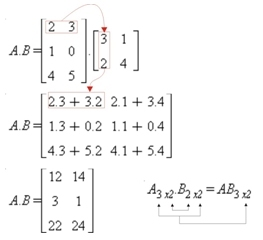
\includegraphics[width=0.5\linewidth]{images/multilicacaoMatricial} 

}

\caption{Multiplicação matricial.}\label{fig:fig-multiplicacao-mat}
\end{figure}

\begin{Shaded}
\begin{Highlighting}[]
\CommentTok{# multiplicação de duas matrizes}
\NormalTok{A <-}\StringTok{ }\KeywordTok{matrix}\NormalTok{(}\KeywordTok{c}\NormalTok{(}\DecValTok{2}\NormalTok{, }\DecValTok{1}\NormalTok{, }\DecValTok{4}\NormalTok{, }\DecValTok{3}\NormalTok{, }\DecValTok{0}\NormalTok{, }\DecValTok{5}\NormalTok{), }\DataTypeTok{ncol =} \DecValTok{2}\NormalTok{)}
\NormalTok{A}
\CommentTok{#>      [,1] [,2]}
\CommentTok{#> [1,]    2    3}
\CommentTok{#> [2,]    1    0}
\CommentTok{#> [3,]    4    5}
\NormalTok{B <-}\StringTok{ }\KeywordTok{matrix}\NormalTok{(}\KeywordTok{c}\NormalTok{(}\DecValTok{3}\NormalTok{, }\DecValTok{2}\NormalTok{, }\DecValTok{1}\NormalTok{, }\DecValTok{4}\NormalTok{), }\DataTypeTok{ncol =} \DecValTok{2}\NormalTok{)}
\NormalTok{B}
\CommentTok{#>      [,1] [,2]}
\CommentTok{#> [1,]    3    1}
\CommentTok{#> [2,]    2    4}
\NormalTok{A }\OperatorTok{*}\StringTok{ }\NormalTok{B  }\CommentTok{# erro pela diferença nas dims entre as matrizes}
\CommentTok{#> Error in A * B: non-conformable arrays}
\NormalTok{prodMat <-}\StringTok{ }\NormalTok{A }\OperatorTok\StringTok{ }\NormalTok{B}
\NormalTok{prodMat}
\CommentTok{#>      [,1] [,2]}
\CommentTok{#> [1,]   12   14}
\CommentTok{#> [2,]    3    1}
\CommentTok{#> [3,]   22   24}
\CommentTok{# multiplicação de uma matriz por um escalar}
\NormalTok{m}
\CommentTok{#>      [,1] [,2] [,3] [,4]}
\CommentTok{#> [1,]    1    2    3    4}
\CommentTok{#> [2,]    5    6    7    8}
\CommentTok{#> [3,]    9   10   11   12}
\CommentTok{#> [4,]   13   14   15   16}
\NormalTok{m }\OperatorTok{*}\StringTok{ }\DecValTok{2}
\CommentTok{#>      [,1] [,2] [,3] [,4]}
\CommentTok{#> [1,]    2    4    6    8}
\CommentTok{#> [2,]   10   12   14   16}
\CommentTok{#> [3,]   18   20   22   24}
\CommentTok{#> [4,]   26   28   30   32}
\end{Highlighting}
\end{Shaded}

\subsubsection{Adição matricial}\label{adicao-matricial}

\begin{Shaded}
\begin{Highlighting}[]
\NormalTok{m}
\CommentTok{#>      [,1] [,2] [,3] [,4]}
\CommentTok{#> [1,]    1    2    3    4}
\CommentTok{#> [2,]    5    6    7    8}
\CommentTok{#> [3,]    9   10   11   12}
\CommentTok{#> [4,]   13   14   15   16}
\NormalTok{m }\OperatorTok{+}\StringTok{ }\NormalTok{m}
\CommentTok{#>      [,1] [,2] [,3] [,4]}
\CommentTok{#> [1,]    2    4    6    8}
\CommentTok{#> [2,]   10   12   14   16}
\CommentTok{#> [3,]   18   20   22   24}
\CommentTok{#> [4,]   26   28   30   32}
\end{Highlighting}
\end{Shaded}

\subsubsection{Produto escalar}\label{produto-escalar}

\begin{Shaded}
\begin{Highlighting}[]
\NormalTok{u <-}\StringTok{ }\DecValTok{1}\OperatorTok{:}\DecValTok{3}
\NormalTok{v <-}\StringTok{ }\KeywordTok{c}\NormalTok{(}\DecValTok{5}\NormalTok{, }\DecValTok{12}\NormalTok{, }\DecValTok{13}\NormalTok{)}
\NormalTok{u }\OperatorTok{*}\StringTok{ }\NormalTok{v}
\CommentTok{#> [1]  5 24 39}
\CommentTok{# produto escalar = u.v = 1*5 + 2*12 + 3*13}
\KeywordTok{crossprod}\NormalTok{(u, v)}
\CommentTok{#>      [,1]}
\CommentTok{#> [1,]   68}
\end{Highlighting}
\end{Shaded}

\subsubsection{Determinante}\label{determinante}

\begin{Shaded}
\begin{Highlighting}[]
\CommentTok{# matriz exemplo}
\NormalTok{mat_ex <-}\StringTok{ }\KeywordTok{matrix}\NormalTok{(}\KeywordTok{c}\NormalTok{(}\DecValTok{1}\NormalTok{, }\OperatorTok{-}\DecValTok{7}\NormalTok{, }\DecValTok{3}\NormalTok{, }\DecValTok{5}\NormalTok{, }\OperatorTok{-}\DecValTok{9}\NormalTok{, }\DecValTok{2}\NormalTok{, }\DecValTok{6}\NormalTok{, }\DecValTok{6}\NormalTok{, }\DecValTok{1}\NormalTok{), }\DataTypeTok{ncol =} \DecValTok{3}\NormalTok{)}
\KeywordTok{det}\NormalTok{(mat_ex)}
\CommentTok{#> [1] 182}
\end{Highlighting}
\end{Shaded}

\subsubsection{Solução de sistemas
lineares}\label{solucao-de-sistemas-lineares}

x1 + x2 = 2

-x1 + x2 = 4

Qual os valores de x1 e x2?

\begin{Shaded}
\begin{Highlighting}[]
\CommentTok{# matrizes do sistema linear}
\NormalTok{coefs <-}\StringTok{ }\KeywordTok{matrix}\NormalTok{(}\KeywordTok{c}\NormalTok{(}\DecValTok{1}\NormalTok{, }\OperatorTok{-}\DecValTok{1}\NormalTok{, }\DecValTok{1}\NormalTok{, }\DecValTok{1}\NormalTok{), }\DataTypeTok{ncol =} \DecValTok{2}\NormalTok{)}
\NormalTok{y <-}\StringTok{ }\KeywordTok{c}\NormalTok{(}\DecValTok{2}\NormalTok{, }\DecValTok{4}\NormalTok{)}
\NormalTok{x <-}\StringTok{ }\KeywordTok{solve}\NormalTok{(coefs, y)}
\NormalTok{x}
\CommentTok{#> [1] -1  3}
\end{Highlighting}
\end{Shaded}

\subsection{\texorpdfstring{Conversão de \texttt{matrix} para
\texttt{vector}}{Conversão de matrix para vector}}\label{conversao-de-matrix-para-vector}

Frequentemente é mais conveniente trabalhar com um vetor do que com uma
matriz, por isso precisamos saber como fazer o caminho inverso. Quando
criamos uma matriz (p.~ex.: \texttt{temp\_mat}) no início da seção ela
foi baseada em um vetor (\texttt{vtemp}). Como fazemos para voltar
aquele vetor original a partir da matriz?

\begin{Shaded}
\begin{Highlighting}[]
\CommentTok{# desmanchando matrizes}
\NormalTok{mel}
\CommentTok{#>      [,1]  [,2]  [,3]  [,4] }
\CommentTok{#> [1,] "m11" "m12" "m13" "m14"}
\CommentTok{#> [2,] "m21" "m22" "m23" "m24"}
\CommentTok{#> [3,] "m31" "m32" "m33" "m34"}
\CommentTok{#> [4,] "m41" "m42" "m43" "m44"}
\CommentTok{# note as diferenças}
\NormalTok{mel[}\DecValTok{1}\NormalTok{, }\DecValTok{1}\NormalTok{]}
\CommentTok{#> [1] "m11"}
\NormalTok{mel[}\DecValTok{1}\NormalTok{]}
\CommentTok{#> [1] "m11"}
\CommentTok{# resulta em uma submatriz}
\NormalTok{mel[}\DecValTok{1}\OperatorTok{:}\DecValTok{4}\NormalTok{, }\DecValTok{1}\OperatorTok{:}\DecValTok{4}\NormalTok{]}
\CommentTok{#>      [,1]  [,2]  [,3]  [,4] }
\CommentTok{#> [1,] "m11" "m12" "m13" "m14"}
\CommentTok{#> [2,] "m21" "m22" "m23" "m24"}
\CommentTok{#> [3,] "m31" "m32" "m33" "m34"}
\CommentTok{#> [4,] "m41" "m42" "m43" "m44"}
\CommentTok{# resulta em um vetor}
\NormalTok{mel[}\DecValTok{1}\OperatorTok{:}\DecValTok{4}\NormalTok{]}
\CommentTok{#> [1] "m11" "m21" "m31" "m41"}
\CommentTok{# submatriz da temp_mat}
\NormalTok{temp_mat[}\DecValTok{1}\OperatorTok{:}\DecValTok{3}\NormalTok{, }\DecValTok{1}\OperatorTok{:}\DecValTok{3}\NormalTok{]}
\CommentTok{#>           Jan   Fev   Mar}
\CommentTok{#> ano1990 25.00 23.20 22.50}
\CommentTok{#> ano1991 24.89 24.07 23.56}
\CommentTok{#> ano1992 23.20 26.61 18.00}
\CommentTok{# vetor gerado de 3 elementos de mat}
\NormalTok{temp_mat[}\DecValTok{1}\OperatorTok{:}\DecValTok{3}\NormalTok{]}
\CommentTok{#> [1] 25.00 24.89 23.20}
\CommentTok{# número de elementos na matriz}
\NormalTok{nel <-}\StringTok{ }\KeywordTok{nrow}\NormalTok{(temp_mat) }\OperatorTok{*}\StringTok{ }\KeywordTok{ncol}\NormalTok{(temp_mat)}
\NormalTok{nel}
\CommentTok{#> [1] 36}
\NormalTok{temp_mat[}\DecValTok{1}\OperatorTok{:}\KeywordTok{nrow}\NormalTok{(temp_mat) }\OperatorTok{*}\StringTok{ }\KeywordTok{ncol}\NormalTok{(temp_mat) ]}
\CommentTok{#> [1] 23.11 21.45 20.08}
\CommentTok{# vetor de temperaturas}
\NormalTok{vtemp <-}\StringTok{ }\NormalTok{temp_mat[}\DecValTok{1}\OperatorTok{:}\NormalTok{(}\KeywordTok{ncol}\NormalTok{(temp_mat) }\OperatorTok{*}\StringTok{ }\KeywordTok{nrow}\NormalTok{(temp_mat))]}
\NormalTok{vtemp}
\CommentTok{#>  [1] 25.00 24.89 23.20 23.20 24.07 26.61 22.50 23.56 18.00 21.00 23.11}
\CommentTok{#> [12] 23.11 19.00 18.29 26.80 17.60 18.22 21.30 18.00 16.72 18.22 19.70}
\CommentTok{#> [23] 19.37 21.45 21.30 20.08 19.70 22.00 21.45 22.50 24.00 26.61 24.07}
\CommentTok{#> [34] 26.80 25.99 20.08}
\CommentTok{# outra forma de converte temp_mat para vetor}
\KeywordTok{c}\NormalTok{(temp_mat)}
\CommentTok{#>  [1] 25.00 24.89 23.20 23.20 24.07 26.61 22.50 23.56 18.00 21.00 23.11}
\CommentTok{#> [12] 23.11 19.00 18.29 26.80 17.60 18.22 21.30 18.00 16.72 18.22 19.70}
\CommentTok{#> [23] 19.37 21.45 21.30 20.08 19.70 22.00 21.45 22.50 24.00 26.61 24.07}
\CommentTok{#> [34] 26.80 25.99 20.08}
\CommentTok{# função formal para converter}
\KeywordTok{as.vector}\NormalTok{(temp_mat)}
\CommentTok{#>  [1] 25.00 24.89 23.20 23.20 24.07 26.61 22.50 23.56 18.00 21.00 23.11}
\CommentTok{#> [12] 23.11 19.00 18.29 26.80 17.60 18.22 21.30 18.00 16.72 18.22 19.70}
\CommentTok{#> [23] 19.37 21.45 21.30 20.08 19.70 22.00 21.45 22.50 24.00 26.61 24.07}
\CommentTok{#> [34] 26.80 25.99 20.08}
\CommentTok{# para desmanchar a matriz com os elementos seguindo a ordem das linhas}
\KeywordTok{c}\NormalTok{(}\KeywordTok{t}\NormalTok{(temp_mat))}
\CommentTok{#>  [1] 25.00 23.20 22.50 21.00 19.00 17.60 18.00 19.70 21.30 22.00 24.00}
\CommentTok{#> [12] 26.80 24.89 24.07 23.56 23.11 18.29 18.22 16.72 19.37 20.08 21.45}
\CommentTok{#> [23] 26.61 25.99 23.20 26.61 18.00 23.11 26.80 21.30 18.22 21.45 19.70}
\CommentTok{#> [34] 22.50 24.07 20.08}
\KeywordTok{as.vector}\NormalTok{(}\KeywordTok{t}\NormalTok{(temp_mat))}
\CommentTok{#>  [1] 25.00 23.20 22.50 21.00 19.00 17.60 18.00 19.70 21.30 22.00 24.00}
\CommentTok{#> [12] 26.80 24.89 24.07 23.56 23.11 18.29 18.22 16.72 19.37 20.08 21.45}
\CommentTok{#> [23] 26.61 25.99 23.20 26.61 18.00 23.11 26.80 21.30 18.22 21.45 19.70}
\CommentTok{#> [34] 22.50 24.07 20.08}
\CommentTok{# serie temporal de temp_mat}
\NormalTok{stemp <-}\StringTok{ }\KeywordTok{c}\NormalTok{(}\KeywordTok{t}\NormalTok{(temp_mat))}
\KeywordTok{plot}\NormalTok{(stemp, }\DataTypeTok{type =} \StringTok{"o"}\NormalTok{)}
\end{Highlighting}
\end{Shaded}

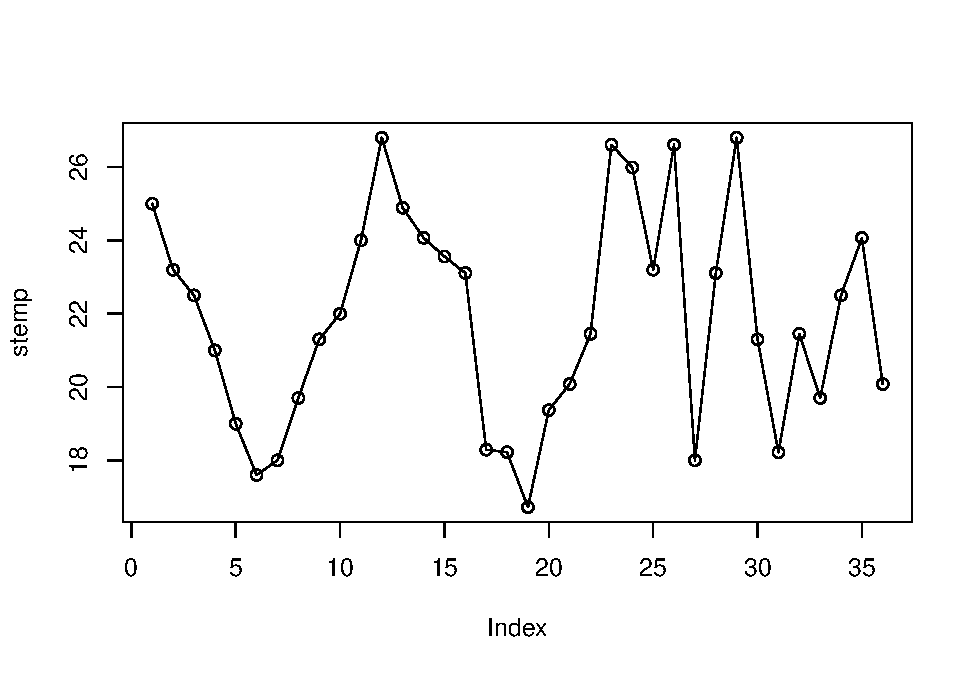
\includegraphics{images/Chunk171-1.pdf}

\begin{Shaded}
\begin{Highlighting}[]
\CommentTok{# criar matriz com colunas temp e meses 1:12}
\KeywordTok{cbind}\NormalTok{(}\KeywordTok{rep}\NormalTok{(}\DecValTok{1}\OperatorTok{:}\DecValTok{12}\NormalTok{, }\KeywordTok{nrow}\NormalTok{(temp_mat)), stemp)}
\CommentTok{#>          stemp}
\CommentTok{#>  [1,]  1 25.00}
\CommentTok{#>  [2,]  2 23.20}
\CommentTok{#>  [3,]  3 22.50}
\CommentTok{#>  [4,]  4 21.00}
\CommentTok{#>  [5,]  5 19.00}
\CommentTok{#>  [6,]  6 17.60}
\CommentTok{#>  [7,]  7 18.00}
\CommentTok{#>  [8,]  8 19.70}
\CommentTok{#>  [9,]  9 21.30}
\CommentTok{#> [10,] 10 22.00}
\CommentTok{#> [11,] 11 24.00}
\CommentTok{#> [12,] 12 26.80}
\CommentTok{#> [13,]  1 24.89}
\CommentTok{#> [14,]  2 24.07}
\CommentTok{#> [15,]  3 23.56}
\CommentTok{#> [16,]  4 23.11}
\CommentTok{#> [17,]  5 18.29}
\CommentTok{#> [18,]  6 18.22}
\CommentTok{#> [19,]  7 16.72}
\CommentTok{#> [20,]  8 19.37}
\CommentTok{#> [21,]  9 20.08}
\CommentTok{#> [22,] 10 21.45}
\CommentTok{#> [23,] 11 26.61}
\CommentTok{#> [24,] 12 25.99}
\CommentTok{#> [25,]  1 23.20}
\CommentTok{#> [26,]  2 26.61}
\CommentTok{#> [27,]  3 18.00}
\CommentTok{#> [28,]  4 23.11}
\CommentTok{#> [29,]  5 26.80}
\CommentTok{#> [30,]  6 21.30}
\CommentTok{#> [31,]  7 18.22}
\CommentTok{#> [32,]  8 21.45}
\CommentTok{#> [33,]  9 19.70}
\CommentTok{#> [34,] 10 22.50}
\CommentTok{#> [35,] 11 24.07}
\CommentTok{#> [36,] 12 20.08}
\CommentTok{# dados de temp e meses}
\NormalTok{tempdat <-}\StringTok{ }\KeywordTok{cbind}\NormalTok{(}\DecValTok{1}\OperatorTok{:}\DecValTok{12}\NormalTok{, stemp)}
\CommentTok{# plot da temperatura pelos meses (os meses repetem)}
\KeywordTok{plot}\NormalTok{(}
\NormalTok{  tempdat,}
  \DataTypeTok{type =} \StringTok{"p"}\NormalTok{, }\CommentTok{# tipo de grafico: pontos}
  \DataTypeTok{pch =} \DecValTok{20}\NormalTok{, }\CommentTok{# codigo numérico do simbolo do ponto}
  \DataTypeTok{col =} \KeywordTok{rep}\NormalTok{(}\DecValTok{1}\OperatorTok{:}\DecValTok{3}\NormalTok{, }\DataTypeTok{each =} \KeywordTok{ncol}\NormalTok{(temp_mat)), }\CommentTok{# cores dos pontos}
  \DataTypeTok{cex =} \KeywordTok{rep}\NormalTok{(}\KeywordTok{seq}\NormalTok{(}\DecValTok{1}\NormalTok{, }\DecValTok{2}\NormalTok{, }\DataTypeTok{by =} \FloatTok{0.5}\NormalTok{), }\DataTypeTok{each =} \KeywordTok{ncol}\NormalTok{(temp_mat)), }\CommentTok{# aumenta tamanho dos pontos}
  \DataTypeTok{las =} \DecValTok{1}\NormalTok{, }\CommentTok{# orientação dos labels dos eixos perpendiculares ao eixo}
  \DataTypeTok{ylab =} \KeywordTok{expression}\NormalTok{(Tar }\OperatorTok{~}\StringTok{ }\NormalTok{(degree }\OperatorTok{~}\StringTok{ }\NormalTok{C)), }\CommentTok{# label da variável y}
  \DataTypeTok{xlab =} \StringTok{"meses"}\NormalTok{, }\CommentTok{# label da variavel x}
  \DataTypeTok{main =} \StringTok{"Temperatura mensal (1990-1992)"} \CommentTok{# título}
\NormalTok{) }\CommentTok{# end plot}
\end{Highlighting}
\end{Shaded}

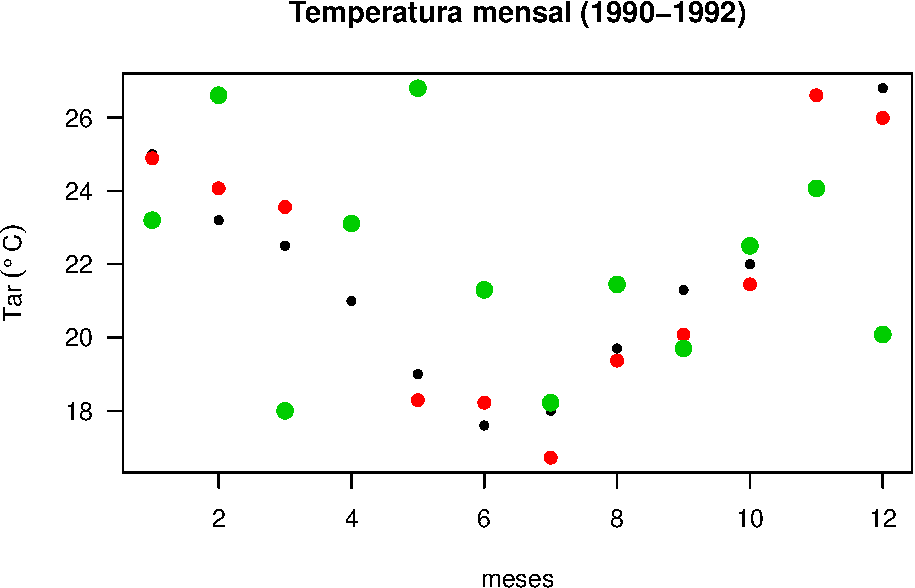
\includegraphics{images/Chunk171-2.pdf}

\begin{Shaded}
\begin{Highlighting}[]
\CommentTok{# para entender a variação nas cores e símbolos usadas no gráfico}
\KeywordTok{cbind}\NormalTok{(}
  \DataTypeTok{meses =} \DecValTok{1}\OperatorTok{:}\DecValTok{12}\NormalTok{, }\DataTypeTok{temp =}\NormalTok{ stemp,}
  \DataTypeTok{cores =} \KeywordTok{rep}\NormalTok{(}\DecValTok{1}\OperatorTok{:}\DecValTok{3}\NormalTok{, }\DataTypeTok{each =} \KeywordTok{ncol}\NormalTok{(temp_mat)), }\CommentTok{# cores}
  \DataTypeTok{simb_tam =} \KeywordTok{rep}\NormalTok{(}\KeywordTok{seq}\NormalTok{(}\DecValTok{1}\NormalTok{, }\DecValTok{2}\NormalTok{, }\DataTypeTok{by =} \FloatTok{0.5}\NormalTok{), }\DataTypeTok{each =} \KeywordTok{ncol}\NormalTok{(temp_mat))}
\NormalTok{) }\CommentTok{# tamanho dos símbolos}
\CommentTok{#>       meses  temp cores simb_tam}
\CommentTok{#>  [1,]     1 25.00     1      1.0}
\CommentTok{#>  [2,]     2 23.20     1      1.0}
\CommentTok{#>  [3,]     3 22.50     1      1.0}
\CommentTok{#>  [4,]     4 21.00     1      1.0}
\CommentTok{#>  [5,]     5 19.00     1      1.0}
\CommentTok{#>  [6,]     6 17.60     1      1.0}
\CommentTok{#>  [7,]     7 18.00     1      1.0}
\CommentTok{#>  [8,]     8 19.70     1      1.0}
\CommentTok{#>  [9,]     9 21.30     1      1.0}
\CommentTok{#> [10,]    10 22.00     1      1.0}
\CommentTok{#> [11,]    11 24.00     1      1.0}
\CommentTok{#> [12,]    12 26.80     1      1.0}
\CommentTok{#> [13,]     1 24.89     2      1.5}
\CommentTok{#> [14,]     2 24.07     2      1.5}
\CommentTok{#> [15,]     3 23.56     2      1.5}
\CommentTok{#> [16,]     4 23.11     2      1.5}
\CommentTok{#> [17,]     5 18.29     2      1.5}
\CommentTok{#> [18,]     6 18.22     2      1.5}
\CommentTok{#> [19,]     7 16.72     2      1.5}
\CommentTok{#> [20,]     8 19.37     2      1.5}
\CommentTok{#> [21,]     9 20.08     2      1.5}
\CommentTok{#> [22,]    10 21.45     2      1.5}
\CommentTok{#> [23,]    11 26.61     2      1.5}
\CommentTok{#> [24,]    12 25.99     2      1.5}
\CommentTok{#> [25,]     1 23.20     3      2.0}
\CommentTok{#> [26,]     2 26.61     3      2.0}
\CommentTok{#> [27,]     3 18.00     3      2.0}
\CommentTok{#> [28,]     4 23.11     3      2.0}
\CommentTok{#> [29,]     5 26.80     3      2.0}
\CommentTok{#> [30,]     6 21.30     3      2.0}
\CommentTok{#> [31,]     7 18.22     3      2.0}
\CommentTok{#> [32,]     8 21.45     3      2.0}
\CommentTok{#> [33,]     9 19.70     3      2.0}
\CommentTok{#> [34,]    10 22.50     3      2.0}
\CommentTok{#> [35,]    11 24.07     3      2.0}
\CommentTok{#> [36,]    12 20.08     3      2.0}
\end{Highlighting}
\end{Shaded}

\section{Array}\label{array}

\emph{Arrays} são multidimensionais. As matrizes são um caso particular
de \emph{arrays} com 2 dimensões: linhas e colunas. Mas podemos ter
dados com \emph{n} dimensões. Por exemplo, imagine o campo espacial de
uma variável meteorológica. Uma matriz com valores de temperatura onde
as colunas representam as longitudes e as linhas as latitudes. A esse
campo pode ser associado um tempo em que a matriz de temperatura
representa o estado térmico espacial daquele momento. Então podemos
dizer que essa \emph{array} possui 3 dimensões:

\begin{itemize}
\item
  latitude (linha)
\item
  longitude (coluna)
\item
  tempo (camadas)
\end{itemize}

\subsection{Criação}\label{criacao-1}

Suponha os campos espaciais médios mensais de temperatura dados pelo
vetor \texttt{temp\_vetor}.

\begin{Shaded}
\begin{Highlighting}[]
\NormalTok{temp_vetor <-}\StringTok{ }\DecValTok{1}\OperatorTok{:}\DecValTok{12}
\NormalTok{temp_vetor}
\CommentTok{#>  [1]  1  2  3  4  5  6  7  8  9 10 11 12}
\CommentTok{# ou}
\NormalTok{temp_array <-}\StringTok{ }\KeywordTok{array}\NormalTok{(}\DataTypeTok{data =}\NormalTok{ temp_vetor, }\DataTypeTok{dim =} \KeywordTok{c}\NormalTok{(}\DecValTok{3}\NormalTok{, }\DecValTok{4}\NormalTok{, }\DecValTok{3}\NormalTok{))}
\NormalTok{temp_array}
\CommentTok{#> , , 1}
\CommentTok{#> }
\CommentTok{#>      [,1] [,2] [,3] [,4]}
\CommentTok{#> [1,]    1    4    7   10}
\CommentTok{#> [2,]    2    5    8   11}
\CommentTok{#> [3,]    3    6    9   12}
\CommentTok{#> }
\CommentTok{#> , , 2}
\CommentTok{#> }
\CommentTok{#>      [,1] [,2] [,3] [,4]}
\CommentTok{#> [1,]    1    4    7   10}
\CommentTok{#> [2,]    2    5    8   11}
\CommentTok{#> [3,]    3    6    9   12}
\CommentTok{#> }
\CommentTok{#> , , 3}
\CommentTok{#> }
\CommentTok{#>      [,1] [,2] [,3] [,4]}
\CommentTok{#> [1,]    1    4    7   10}
\CommentTok{#> [2,]    2    5    8   11}
\CommentTok{#> [3,]    3    6    9   12}
\KeywordTok{dim}\NormalTok{(temp_array)}
\CommentTok{#> [1] 3 4 3}
\KeywordTok{length}\NormalTok{(temp_array)}
\CommentTok{#> [1] 36}
\KeywordTok{class}\NormalTok{(temp_array)}
\CommentTok{#> [1] "array"}
\KeywordTok{mode}\NormalTok{(temp_array)}
\CommentTok{#> [1] "numeric"}
\end{Highlighting}
\end{Shaded}

\subsection{Indexação}\label{indexacao}

\begin{Shaded}
\begin{Highlighting}[]
\KeywordTok{colnames}\NormalTok{(temp_array) <-}\StringTok{ }\OperatorTok{-}\DecValTok{45}\OperatorTok{:-}\DecValTok{42}
\KeywordTok{rownames}\NormalTok{(temp_array) <-}\StringTok{ }\OperatorTok{-}\DecValTok{19}\OperatorTok{:-}\DecValTok{21}
\NormalTok{temp_array}
\CommentTok{#> , , 1}
\CommentTok{#> }
\CommentTok{#>     -45 -44 -43 -42}
\CommentTok{#> -19   1   4   7  10}
\CommentTok{#> -20   2   5   8  11}
\CommentTok{#> -21   3   6   9  12}
\CommentTok{#> }
\CommentTok{#> , , 2}
\CommentTok{#> }
\CommentTok{#>     -45 -44 -43 -42}
\CommentTok{#> -19   1   4   7  10}
\CommentTok{#> -20   2   5   8  11}
\CommentTok{#> -21   3   6   9  12}
\CommentTok{#> }
\CommentTok{#> , , 3}
\CommentTok{#> }
\CommentTok{#>     -45 -44 -43 -42}
\CommentTok{#> -19   1   4   7  10}
\CommentTok{#> -20   2   5   8  11}
\CommentTok{#> -21   3   6   9  12}
\end{Highlighting}
\end{Shaded}

Podemos usar as mesmos procedimentos de indexação de uma \texttt{matrix}
para seleção de partes de uma \texttt{array}.

\begin{Shaded}
\begin{Highlighting}[]
\CommentTok{# serie temporal do 1º ponto}
\NormalTok{temp_array[}\DecValTok{1}\NormalTok{, }\DecValTok{1}\NormalTok{, ]}
\CommentTok{#> [1] 1 1 1}
\NormalTok{temp_array[}\StringTok{"-19"}\NormalTok{, }\StringTok{"-45"}\NormalTok{, ]}
\CommentTok{#> [1] 1 1 1}
\CommentTok{# para 1a faixa de latitude (-19),}
\CommentTok{# os valores de temp das longitudes em todos tempos}
\NormalTok{temp_array[}\DecValTok{1}\NormalTok{, , ]}
\CommentTok{#>     [,1] [,2] [,3]}
\CommentTok{#> -45    1    1    1}
\CommentTok{#> -44    4    4    4}
\CommentTok{#> -43    7    7    7}
\CommentTok{#> -42   10   10   10}
\CommentTok{# para 2a faixa de longitude (-44), todas longitudes e tempos}
\NormalTok{temp_array[, }\DecValTok{2}\NormalTok{, ]}
\CommentTok{#>     [,1] [,2] [,3]}
\CommentTok{#> -19    4    4    4}
\CommentTok{#> -20    5    5    5}
\CommentTok{#> -21    6    6    6}
\CommentTok{# média meridional}
\KeywordTok{colMeans}\NormalTok{(temp_array[, }\DecValTok{2}\NormalTok{, ])}
\CommentTok{#> [1] 5 5 5}
\CommentTok{# subdominio "espacial"}
\NormalTok{temp_array[}\DecValTok{2}\OperatorTok{:}\DecValTok{3}\NormalTok{, }\DecValTok{2}\OperatorTok{:}\DecValTok{3}\NormalTok{, ]}
\CommentTok{#> , , 1}
\CommentTok{#> }
\CommentTok{#>     -44 -43}
\CommentTok{#> -20   5   8}
\CommentTok{#> -21   6   9}
\CommentTok{#> }
\CommentTok{#> , , 2}
\CommentTok{#> }
\CommentTok{#>     -44 -43}
\CommentTok{#> -20   5   8}
\CommentTok{#> -21   6   9}
\CommentTok{#> }
\CommentTok{#> , , 3}
\CommentTok{#> }
\CommentTok{#>     -44 -43}
\CommentTok{#> -20   5   8}
\CommentTok{#> -21   6   9}
\CommentTok{# média espacial do 1o mês}
\KeywordTok{mean}\NormalTok{(temp_array[, , }\DecValTok{1}\NormalTok{])}
\CommentTok{#> [1] 6.5}
\CommentTok{# média espacial do segundo mês}
\KeywordTok{mean}\NormalTok{(temp_array[, , }\DecValTok{2}\NormalTok{])}
\CommentTok{#> [1] 6.5}
\CommentTok{# demanchando uma array (conversão para vetor)}
\KeywordTok{c}\NormalTok{(temp_array)}
\CommentTok{#>  [1]  1  2  3  4  5  6  7  8  9 10 11 12  1  2  3  4  5  6  7  8  9 10 11}
\CommentTok{#> [24] 12  1  2  3  4  5  6  7  8  9 10 11 12}
\KeywordTok{c}\NormalTok{(temp_array[, , }\DecValTok{1}\NormalTok{])}
\CommentTok{#>  [1]  1  2  3  4  5  6  7  8  9 10 11 12}
\CommentTok{# para entender a forma como a matriz é convertida para vetor}
\NormalTok{mat_temp <-}\StringTok{ }\KeywordTok{cbind}\NormalTok{(}
  \DataTypeTok{mes =} \KeywordTok{rep}\NormalTok{(}\DecValTok{1}\OperatorTok{:}\DecValTok{3}\NormalTok{, }\DataTypeTok{each =} \DecValTok{20}\NormalTok{),}
  \DataTypeTok{elemat =} \KeywordTok{rep}\NormalTok{(}\DecValTok{1}\OperatorTok{:}\DecValTok{20}\NormalTok{, }\DataTypeTok{times =} \DecValTok{6}\NormalTok{),}
  \DataTypeTok{valores =} \KeywordTok{c}\NormalTok{(temp_array),}
  \DataTypeTok{elearr =} \DecValTok{1}\OperatorTok{:}\NormalTok{(}\KeywordTok{cumprod}\NormalTok{(}\KeywordTok{dim}\NormalTok{(temp_array))[}\DecValTok{3}\NormalTok{])}
\NormalTok{)}
\CommentTok{#> Warning in cbind(mes = rep(1:3, each = 20), elemat = rep(1:20, times =}
\CommentTok{#> 6), : number of rows of result is not a multiple of vector length (arg 3)}
\NormalTok{mat_temp}
\CommentTok{#>        mes elemat valores elearr}
\CommentTok{#>   [1,]   1      1       1      1}
\CommentTok{#>   [2,]   1      2       2      2}
\CommentTok{#>   [3,]   1      3       3      3}
\CommentTok{#>   [4,]   1      4       4      4}
\CommentTok{#>   [5,]   1      5       5      5}
\CommentTok{#>   [6,]   1      6       6      6}
\CommentTok{#>   [7,]   1      7       7      7}
\CommentTok{#>   [8,]   1      8       8      8}
\CommentTok{#>   [9,]   1      9       9      9}
\CommentTok{#>  [10,]   1     10      10     10}
\CommentTok{#>  [11,]   1     11      11     11}
\CommentTok{#>  [12,]   1     12      12     12}
\CommentTok{#>  [13,]   1     13       1     13}
\CommentTok{#>  [14,]   1     14       2     14}
\CommentTok{#>  [15,]   1     15       3     15}
\CommentTok{#>  [16,]   1     16       4     16}
\CommentTok{#>  [17,]   1     17       5     17}
\CommentTok{#>  [18,]   1     18       6     18}
\CommentTok{#>  [19,]   1     19       7     19}
\CommentTok{#>  [20,]   1     20       8     20}
\CommentTok{#>  [21,]   2      1       9     21}
\CommentTok{#>  [22,]   2      2      10     22}
\CommentTok{#>  [23,]   2      3      11     23}
\CommentTok{#>  [24,]   2      4      12     24}
\CommentTok{#>  [25,]   2      5       1     25}
\CommentTok{#>  [26,]   2      6       2     26}
\CommentTok{#>  [27,]   2      7       3     27}
\CommentTok{#>  [28,]   2      8       4     28}
\CommentTok{#>  [29,]   2      9       5     29}
\CommentTok{#>  [30,]   2     10       6     30}
\CommentTok{#>  [31,]   2     11       7     31}
\CommentTok{#>  [32,]   2     12       8     32}
\CommentTok{#>  [33,]   2     13       9     33}
\CommentTok{#>  [34,]   2     14      10     34}
\CommentTok{#>  [35,]   2     15      11     35}
\CommentTok{#>  [36,]   2     16      12     36}
\CommentTok{#>  [37,]   2     17       1      1}
\CommentTok{#>  [38,]   2     18       2      2}
\CommentTok{#>  [39,]   2     19       3      3}
\CommentTok{#>  [40,]   2     20       4      4}
\CommentTok{#>  [41,]   3      1       5      5}
\CommentTok{#>  [42,]   3      2       6      6}
\CommentTok{#>  [43,]   3      3       7      7}
\CommentTok{#>  [44,]   3      4       8      8}
\CommentTok{#>  [45,]   3      5       9      9}
\CommentTok{#>  [46,]   3      6      10     10}
\CommentTok{#>  [47,]   3      7      11     11}
\CommentTok{#>  [48,]   3      8      12     12}
\CommentTok{#>  [49,]   3      9       1     13}
\CommentTok{#>  [50,]   3     10       2     14}
\CommentTok{#>  [51,]   3     11       3     15}
\CommentTok{#>  [52,]   3     12       4     16}
\CommentTok{#>  [53,]   3     13       5     17}
\CommentTok{#>  [54,]   3     14       6     18}
\CommentTok{#>  [55,]   3     15       7     19}
\CommentTok{#>  [56,]   3     16       8     20}
\CommentTok{#>  [57,]   3     17       9     21}
\CommentTok{#>  [58,]   3     18      10     22}
\CommentTok{#>  [59,]   3     19      11     23}
\CommentTok{#>  [60,]   3     20      12     24}
\CommentTok{#>  [61,]   1      1       1     25}
\CommentTok{#>  [62,]   1      2       2     26}
\CommentTok{#>  [63,]   1      3       3     27}
\CommentTok{#>  [64,]   1      4       4     28}
\CommentTok{#>  [65,]   1      5       5     29}
\CommentTok{#>  [66,]   1      6       6     30}
\CommentTok{#>  [67,]   1      7       7     31}
\CommentTok{#>  [68,]   1      8       8     32}
\CommentTok{#>  [69,]   1      9       9     33}
\CommentTok{#>  [70,]   1     10      10     34}
\CommentTok{#>  [71,]   1     11      11     35}
\CommentTok{#>  [72,]   1     12      12     36}
\CommentTok{#>  [73,]   1     13       1      1}
\CommentTok{#>  [74,]   1     14       2      2}
\CommentTok{#>  [75,]   1     15       3      3}
\CommentTok{#>  [76,]   1     16       4      4}
\CommentTok{#>  [77,]   1     17       5      5}
\CommentTok{#>  [78,]   1     18       6      6}
\CommentTok{#>  [79,]   1     19       7      7}
\CommentTok{#>  [80,]   1     20       8      8}
\CommentTok{#>  [81,]   2      1       9      9}
\CommentTok{#>  [82,]   2      2      10     10}
\CommentTok{#>  [83,]   2      3      11     11}
\CommentTok{#>  [84,]   2      4      12     12}
\CommentTok{#>  [85,]   2      5       1     13}
\CommentTok{#>  [86,]   2      6       2     14}
\CommentTok{#>  [87,]   2      7       3     15}
\CommentTok{#>  [88,]   2      8       4     16}
\CommentTok{#>  [89,]   2      9       5     17}
\CommentTok{#>  [90,]   2     10       6     18}
\CommentTok{#>  [91,]   2     11       7     19}
\CommentTok{#>  [92,]   2     12       8     20}
\CommentTok{#>  [93,]   2     13       9     21}
\CommentTok{#>  [94,]   2     14      10     22}
\CommentTok{#>  [95,]   2     15      11     23}
\CommentTok{#>  [96,]   2     16      12     24}
\CommentTok{#>  [97,]   2     17       1     25}
\CommentTok{#>  [98,]   2     18       2     26}
\CommentTok{#>  [99,]   2     19       3     27}
\CommentTok{#> [100,]   2     20       4     28}
\CommentTok{#> [101,]   3      1       5     29}
\CommentTok{#> [102,]   3      2       6     30}
\CommentTok{#> [103,]   3      3       7     31}
\CommentTok{#> [104,]   3      4       8     32}
\CommentTok{#> [105,]   3      5       9     33}
\CommentTok{#> [106,]   3      6      10     34}
\CommentTok{#> [107,]   3      7      11     35}
\CommentTok{#> [108,]   3      8      12     36}
\CommentTok{#> [109,]   3      9       1      1}
\CommentTok{#> [110,]   3     10       2      2}
\CommentTok{#> [111,]   3     11       3      3}
\CommentTok{#> [112,]   3     12       4      4}
\CommentTok{#> [113,]   3     13       5      5}
\CommentTok{#> [114,]   3     14       6      6}
\CommentTok{#> [115,]   3     15       7      7}
\CommentTok{#> [116,]   3     16       8      8}
\CommentTok{#> [117,]   3     17       9      9}
\CommentTok{#> [118,]   3     18      10     10}
\CommentTok{#> [119,]   3     19      11     11}
\CommentTok{#> [120,]   3     20      12     12}
\end{Highlighting}
\end{Shaded}

\section{List}\label{list}

Listas são o segundo tipo de vetor. O primeiro tipo nós já vimos, são os
\textbf{vetores atômicos}, nos quais todos os elementos devem ser de uma
mesma classe de objeto. Listas são uma estrutura de dados muito versátil
por pelo menos 3 razões:

\begin{enumerate}
\def\labelenumi{\arabic{enumi}.}
\tightlist
\item
  Os elementos podem ser de diferentes classes de objetos (p.ex.: um
  elemento \texttt{numeric}, outro \texttt{character});
\item
  Cada elemento pode ter um tamanho diferente;
\item
  Os elementos podem conter diferentes estrutura de dados (p.ex.: um
  elemento \texttt{matrix}, outro \texttt{vector});
\end{enumerate}

Dentro da lista o conjunto de objetos são ordenados e cada elemento pode
conter sub-elementos.

\subsection{Criação}\label{criacao-2}

As vezes precisamos de um \emph{container} para armazenar diferentes
tipos de dados do R e com diferente tamanhos. As \emph{listas} servem
para isso e permitem armazenar qualquer número de itens de qualquer
tipo. Uma lista pode conter números, caracteres ou uma mistura de
\emph{dataframes}, sub-listas, matrizes e vetores.

Listas podem ser criadas com a função \texttt{list()}. A especificação
do conteúdo de uma lista é muito similar a da função \texttt{c()} vista
anteriormente. Nós simplesmente listamos os elementos da lista separados
por uma vírgula dentro da função \texttt{list()}.

\begin{Shaded}
\begin{Highlighting}[]
\CommentTok{# lista de dados heterogêneos}
\NormalTok{lst <-}\StringTok{ }\KeywordTok{list}\NormalTok{(}\DecValTok{1}\OperatorTok{:}\DecValTok{4}\NormalTok{, }\KeywordTok{c}\NormalTok{(}\FloatTok{1.1}\NormalTok{, }\FloatTok{2.3}\NormalTok{, }\FloatTok{5.9}\NormalTok{), }\KeywordTok{c}\NormalTok{(}\OtherTok{TRUE}\NormalTok{, }\OtherTok{FALSE}\NormalTok{), }\StringTok{"R"}\NormalTok{, }\KeywordTok{list}\NormalTok{(}\DecValTok{0}\NormalTok{, }\DecValTok{1}\NormalTok{))}
\NormalTok{lst}
\CommentTok{#> [[1]]}
\CommentTok{#> [1] 1 2 3 4}
\CommentTok{#> }
\CommentTok{#> [[2]]}
\CommentTok{#> [1] 1.1 2.3 5.9}
\CommentTok{#> }
\CommentTok{#> [[3]]}
\CommentTok{#> [1]  TRUE FALSE}
\CommentTok{#> }
\CommentTok{#> [[4]]}
\CommentTok{#> [1] "R"}
\CommentTok{#> }
\CommentTok{#> [[5]]}
\CommentTok{#> [[5]][[1]]}
\CommentTok{#> [1] 0}
\CommentTok{#> }
\CommentTok{#> [[5]][[2]]}
\CommentTok{#> [1] 1}
\CommentTok{# estrutura da lista}
\KeywordTok{str}\NormalTok{(lst)}
\CommentTok{#> List of 5}
\CommentTok{#>  $ : int [1:4] 1 2 3 4}
\CommentTok{#>  $ : num [1:3] 1.1 2.3 5.9}
\CommentTok{#>  $ : logi [1:2] TRUE FALSE}
\CommentTok{#>  $ : chr "R"}
\CommentTok{#>  $ :List of 2}
\CommentTok{#>   ..$ : num 0}
\CommentTok{#>   ..$ : num 1}
\CommentTok{# tamanho da lista (num. de componentes ou elementos)}
\KeywordTok{length}\NormalTok{(lst)}
\CommentTok{#> [1] 5}
\CommentTok{# atribuindo nomes a lista}
\KeywordTok{names}\NormalTok{(lst)}
\CommentTok{#> NULL}
\KeywordTok{names}\NormalTok{(lst) <-}\StringTok{ }\KeywordTok{c}\NormalTok{(}\StringTok{"vetor_int"}\NormalTok{, }\StringTok{"vetor_num"}\NormalTok{, }\StringTok{"logico"}\NormalTok{, }\StringTok{"char"}\NormalTok{, }\StringTok{"lista"}\NormalTok{)}
\end{Highlighting}
\end{Shaded}

Os índices em colchetes duplos \texttt{{[}{[}{]}{]}} identificam o
elemento ou a componente da lista. Os índices em colchete simples
\texttt{{[}{]}} indicam qual sub-elemento da lista está sendo mostrado.
Por exemplo \texttt{1.1} é o primeiro sub-elemento do segundo elemento
da lista \texttt{lst}. Desse aninhamento de elementos surge o sistema de
indexação de listas. A estrutura de uma lista pode se tornar complicada
com o aumento do grau de sub-elementos. Mas essa flexibilidade, faz das
listas uma ferramenta de armazenamento de dados para todos propósitos.

\begin{rmdtip}
Veremos que no R, listas são frequentemente usadas para armazenar a
saída de funções com diversos resultados. Como por exemplo a saída das
funções \texttt{rle()}.
\end{rmdtip}

Para verificar se uma lista é aninhada usamos a função
\texttt{is.recursive()}.

\begin{Shaded}
\begin{Highlighting}[]
\KeywordTok{is.recursive}\NormalTok{(lst)}
\CommentTok{#> [1] TRUE}
\end{Highlighting}
\end{Shaded}

Vamos ver um exemplo onde criamos uma lista com informações de duas
estações meteorológicas.

\begin{Shaded}
\begin{Highlighting}[]
\CommentTok{# matriz de dados meteorológicos da estação de Santa Maria}
\NormalTok{dados_sm <-}\StringTok{ }\KeywordTok{cbind}\NormalTok{(}
  \DataTypeTok{tar =} \KeywordTok{c}\NormalTok{(}\DecValTok{31}\NormalTok{, }\DecValTok{35}\NormalTok{, }\DecValTok{21}\NormalTok{, }\DecValTok{23}\NormalTok{, }\DecValTok{33}\NormalTok{, }\DecValTok{17}\NormalTok{),}
  \DataTypeTok{prec =} \KeywordTok{c}\NormalTok{(}\DecValTok{300}\NormalTok{, }\DecValTok{200}\NormalTok{, }\DecValTok{150}\NormalTok{, }\DecValTok{120}\NormalTok{, }\DecValTok{210}\NormalTok{, }\DecValTok{110}\NormalTok{)}
\NormalTok{)}
\NormalTok{dados_sm}
\CommentTok{#>      tar prec}
\CommentTok{#> [1,]  31  300}
\CommentTok{#> [2,]  35  200}
\CommentTok{#> [3,]  21  150}
\CommentTok{#> [4,]  23  120}
\CommentTok{#> [5,]  33  210}
\CommentTok{#> [6,]  17  110}
\CommentTok{# lista com informações da estação de santa maria}
\NormalTok{sm_l <-}\StringTok{ }\KeywordTok{list}\NormalTok{(}
  \KeywordTok{c}\NormalTok{(}\OperatorTok{-}\DecValTok{45}\NormalTok{, }\OperatorTok{-}\DecValTok{23}\NormalTok{),}
  \StringTok{"Santa Maria"}\NormalTok{,}
\NormalTok{  dados_sm}
\NormalTok{)}
\NormalTok{sm_l}
\CommentTok{#> [[1]]}
\CommentTok{#> [1] -45 -23}
\CommentTok{#> }
\CommentTok{#> [[2]]}
\CommentTok{#> [1] "Santa Maria"}
\CommentTok{#> }
\CommentTok{#> [[3]]}
\CommentTok{#>      tar prec}
\CommentTok{#> [1,]  31  300}
\CommentTok{#> [2,]  35  200}
\CommentTok{#> [3,]  21  150}
\CommentTok{#> [4,]  23  120}
\CommentTok{#> [5,]  33  210}
\CommentTok{#> [6,]  17  110}
\CommentTok{# adicionar nomes aos elementos}
\KeywordTok{names}\NormalTok{(sm_l) <-}\StringTok{ }\KeywordTok{c}\NormalTok{(}\StringTok{"coords"}\NormalTok{, }\StringTok{"cidade"}\NormalTok{, }\StringTok{"dados"}\NormalTok{)}
\NormalTok{sm_l}
\CommentTok{#> $coords}
\CommentTok{#> [1] -45 -23}
\CommentTok{#> }
\CommentTok{#> $cidade}
\CommentTok{#> [1] "Santa Maria"}
\CommentTok{#> }
\CommentTok{#> $dados}
\CommentTok{#>      tar prec}
\CommentTok{#> [1,]  31  300}
\CommentTok{#> [2,]  35  200}
\CommentTok{#> [3,]  21  150}
\CommentTok{#> [4,]  23  120}
\CommentTok{#> [5,]  33  210}
\CommentTok{#> [6,]  17  110}
\CommentTok{# matriz de dados meteorológicos da estação de Júlio de Castilhos}
\NormalTok{dados_jc <-}\StringTok{ }\KeywordTok{cbind}\NormalTok{(}
  \DataTypeTok{tar =} \KeywordTok{c}\NormalTok{(}\FloatTok{22.5}\NormalTok{, }\DecValTok{20}\NormalTok{, }\FloatTok{18.75}\NormalTok{, }\DecValTok{18}\NormalTok{, }\FloatTok{20.25}\NormalTok{, }\FloatTok{17.75}\NormalTok{),}
  \DataTypeTok{prec =} \KeywordTok{c}\NormalTok{(}\DecValTok{360}\NormalTok{, }\DecValTok{310}\NormalTok{, }\DecValTok{285}\NormalTok{, }\DecValTok{270}\NormalTok{, }\DecValTok{315}\NormalTok{, }\DecValTok{265}\NormalTok{)}
\NormalTok{)}
\CommentTok{# criando lista de JC, mas nomeando de forma diferente}
\NormalTok{jc_l <-}\StringTok{ }\KeywordTok{list}\NormalTok{(}
  \DataTypeTok{coords =} \KeywordTok{c}\NormalTok{(}\OperatorTok{-}\FloatTok{45.1}\NormalTok{, }\OperatorTok{-}\FloatTok{23.2}\NormalTok{),}
  \DataTypeTok{cidade =} \StringTok{"Júlio de Castilhos"}\NormalTok{,}
  \DataTypeTok{dados =}\NormalTok{ dados_jc}
\NormalTok{)}
\CommentTok{# adicionar nomes as componentes}
\KeywordTok{names}\NormalTok{(jc_l) <-}\StringTok{ }\KeywordTok{names}\NormalTok{(sm_l)}
\NormalTok{jc_l}
\CommentTok{#> $coords}
\CommentTok{#> [1] -45.1 -23.2}
\CommentTok{#> }
\CommentTok{#> $cidade}
\CommentTok{#> [1] "Júlio de Castilhos"}
\CommentTok{#> }
\CommentTok{#> $dados}
\CommentTok{#>        tar prec}
\CommentTok{#> [1,] 22.50  360}
\CommentTok{#> [2,] 20.00  310}
\CommentTok{#> [3,] 18.75  285}
\CommentTok{#> [4,] 18.00  270}
\CommentTok{#> [5,] 20.25  315}
\CommentTok{#> [6,] 17.75  265}
\end{Highlighting}
\end{Shaded}

As informações de cada estação estão armazenadas em 2 listas. Mas é mais
prático termos todas estações em um única lista:

\begin{Shaded}
\begin{Highlighting}[]
\CommentTok{# combinando listas mantendo os elementos separadamente}
\NormalTok{dados_l <-}\StringTok{ }\KeywordTok{list}\NormalTok{(sm_l, jc_l)}
\NormalTok{dados_l}
\CommentTok{#> [[1]]}
\CommentTok{#> [[1]]$coords}
\CommentTok{#> [1] -45 -23}
\CommentTok{#> }
\CommentTok{#> [[1]]$cidade}
\CommentTok{#> [1] "Santa Maria"}
\CommentTok{#> }
\CommentTok{#> [[1]]$dados}
\CommentTok{#>      tar prec}
\CommentTok{#> [1,]  31  300}
\CommentTok{#> [2,]  35  200}
\CommentTok{#> [3,]  21  150}
\CommentTok{#> [4,]  23  120}
\CommentTok{#> [5,]  33  210}
\CommentTok{#> [6,]  17  110}
\CommentTok{#> }
\CommentTok{#> }
\CommentTok{#> [[2]]}
\CommentTok{#> [[2]]$coords}
\CommentTok{#> [1] -45.1 -23.2}
\CommentTok{#> }
\CommentTok{#> [[2]]$cidade}
\CommentTok{#> [1] "Júlio de Castilhos"}
\CommentTok{#> }
\CommentTok{#> [[2]]$dados}
\CommentTok{#>        tar prec}
\CommentTok{#> [1,] 22.50  360}
\CommentTok{#> [2,] 20.00  310}
\CommentTok{#> [3,] 18.75  285}
\CommentTok{#> [4,] 18.00  270}
\CommentTok{#> [5,] 20.25  315}
\CommentTok{#> [6,] 17.75  265}
\KeywordTok{names}\NormalTok{(dados_l)}
\CommentTok{#> NULL}
\KeywordTok{names}\NormalTok{(dados_l) <-}\StringTok{ }\KeywordTok{c}\NormalTok{(}\StringTok{"sm"}\NormalTok{, }\StringTok{"jc"}\NormalTok{)}
\NormalTok{dados_l}
\CommentTok{#> $sm}
\CommentTok{#> $sm$coords}
\CommentTok{#> [1] -45 -23}
\CommentTok{#> }
\CommentTok{#> $sm$cidade}
\CommentTok{#> [1] "Santa Maria"}
\CommentTok{#> }
\CommentTok{#> $sm$dados}
\CommentTok{#>      tar prec}
\CommentTok{#> [1,]  31  300}
\CommentTok{#> [2,]  35  200}
\CommentTok{#> [3,]  21  150}
\CommentTok{#> [4,]  23  120}
\CommentTok{#> [5,]  33  210}
\CommentTok{#> [6,]  17  110}
\CommentTok{#> }
\CommentTok{#> }
\CommentTok{#> $jc}
\CommentTok{#> $jc$coords}
\CommentTok{#> [1] -45.1 -23.2}
\CommentTok{#> }
\CommentTok{#> $jc$cidade}
\CommentTok{#> [1] "Júlio de Castilhos"}
\CommentTok{#> }
\CommentTok{#> $jc$dados}
\CommentTok{#>        tar prec}
\CommentTok{#> [1,] 22.50  360}
\CommentTok{#> [2,] 20.00  310}
\CommentTok{#> [3,] 18.75  285}
\CommentTok{#> [4,] 18.00  270}
\CommentTok{#> [5,] 20.25  315}
\CommentTok{#> [6,] 17.75  265}
\CommentTok{# como a lista é um tipo vetor, a função length()}
\CommentTok{# fornece o número de elementos da lista}
\KeywordTok{length}\NormalTok{(dados_l)}
\CommentTok{#> [1] 2}
\end{Highlighting}
\end{Shaded}

Para resumir a estrutura de uma lista (ou \emph{dataframe}) podemos usar
a função \texttt{str()}:

\begin{Shaded}
\begin{Highlighting}[]
\KeywordTok{str}\NormalTok{(dados_l)}
\CommentTok{#> List of 2}
\CommentTok{#>  $ sm:List of 3}
\CommentTok{#>   ..$ coords: num [1:2] -45 -23}
\CommentTok{#>   ..$ cidade: chr "Santa Maria"}
\CommentTok{#>   ..$ dados : num [1:6, 1:2] 31 35 21 23 33 17 300 200 150 120 ...}
\CommentTok{#>   .. ..- attr(*, "dimnames")=List of 2}
\CommentTok{#>   .. .. ..$ : NULL}
\CommentTok{#>   .. .. ..$ : chr [1:2] "tar" "prec"}
\CommentTok{#>  $ jc:List of 3}
\CommentTok{#>   ..$ coords: num [1:2] -45.1 -23.2}
\CommentTok{#>   ..$ cidade: chr "Júlio de Castilhos"}
\CommentTok{#>   ..$ dados : num [1:6, 1:2] 22.5 20 18.8 18 20.2 ...}
\CommentTok{#>   .. ..- attr(*, "dimnames")=List of 2}
\CommentTok{#>   .. .. ..$ : NULL}
\CommentTok{#>   .. .. ..$ : chr [1:2] "tar" "prec"}
\end{Highlighting}
\end{Shaded}

As listas também poderiam ser combinadas com função concatena ou combina
\texttt{c()}.

\begin{Shaded}
\begin{Highlighting}[]
\NormalTok{dados_l2 <-}\StringTok{ }\KeywordTok{c}\NormalTok{(sm_l, jc_l)}
\NormalTok{dados_l2}
\CommentTok{#> $coords}
\CommentTok{#> [1] -45 -23}
\CommentTok{#> }
\CommentTok{#> $cidade}
\CommentTok{#> [1] "Santa Maria"}
\CommentTok{#> }
\CommentTok{#> $dados}
\CommentTok{#>      tar prec}
\CommentTok{#> [1,]  31  300}
\CommentTok{#> [2,]  35  200}
\CommentTok{#> [3,]  21  150}
\CommentTok{#> [4,]  23  120}
\CommentTok{#> [5,]  33  210}
\CommentTok{#> [6,]  17  110}
\CommentTok{#> }
\CommentTok{#> $coords}
\CommentTok{#> [1] -45.1 -23.2}
\CommentTok{#> }
\CommentTok{#> $cidade}
\CommentTok{#> [1] "Júlio de Castilhos"}
\CommentTok{#> }
\CommentTok{#> $dados}
\CommentTok{#>        tar prec}
\CommentTok{#> [1,] 22.50  360}
\CommentTok{#> [2,] 20.00  310}
\CommentTok{#> [3,] 18.75  285}
\CommentTok{#> [4,] 18.00  270}
\CommentTok{#> [5,] 20.25  315}
\CommentTok{#> [6,] 17.75  265}
\KeywordTok{str}\NormalTok{(dados_l2)}
\CommentTok{#> List of 6}
\CommentTok{#>  $ coords: num [1:2] -45 -23}
\CommentTok{#>  $ cidade: chr "Santa Maria"}
\CommentTok{#>  $ dados : num [1:6, 1:2] 31 35 21 23 33 17 300 200 150 120 ...}
\CommentTok{#>   ..- attr(*, "dimnames")=List of 2}
\CommentTok{#>   .. ..$ : NULL}
\CommentTok{#>   .. ..$ : chr [1:2] "tar" "prec"}
\CommentTok{#>  $ coords: num [1:2] -45.1 -23.2}
\CommentTok{#>  $ cidade: chr "Júlio de Castilhos"}
\CommentTok{#>  $ dados : num [1:6, 1:2] 22.5 20 18.8 18 20.2 ...}
\CommentTok{#>   ..- attr(*, "dimnames")=List of 2}
\CommentTok{#>   .. ..$ : NULL}
\CommentTok{#>   .. ..$ : chr [1:2] "tar" "prec"}
\end{Highlighting}
\end{Shaded}

\subsection{Indexação}\label{indexacao-1}

\subsubsection{\texorpdfstring{Operador
\texttt{{[}}}{Operador {[}}}\label{operador}

Assim como em vetores, podemos acessar os elementos de uma lista usando
os colchetes \texttt{{[}} com índices numéricos positivos, negativos,
caracteres (nomes dos elementos) e lógicos. As expressões abaixo,
ilustram o uso dessas diferentes formas de seleção de elementos e
produzem o mesmo resultado.

\begin{Shaded}
\begin{Highlighting}[]
\NormalTok{sm_l[}\DecValTok{1}\OperatorTok{:}\DecValTok{2}\NormalTok{]}
\CommentTok{#> $coords}
\CommentTok{#> [1] -45 -23}
\CommentTok{#> }
\CommentTok{#> $cidade}
\CommentTok{#> [1] "Santa Maria"}
\NormalTok{sm_l[}\KeywordTok{c}\NormalTok{(}\StringTok{"coords"}\NormalTok{, }\StringTok{"alt"}\NormalTok{)]}
\CommentTok{#> $coords}
\CommentTok{#> [1] -45 -23}
\CommentTok{#> }
\CommentTok{#> $<NA>}
\CommentTok{#> NULL}
\end{Highlighting}
\end{Shaded}

O resultado da seleção do 1º e 2º elemento é uma lista menor que a
original. Isso não é muito útil, uma vez que muitas funções do R não
lidam com listas. Por exemplo, se quiséssemos calcular a soma do vetor
contido do primeiro elemento da lista \texttt{lst} obtém-se um erro.

\begin{Shaded}
\begin{Highlighting}[]
\CommentTok{# seleção do 1º elemento da lst}
\NormalTok{lst[}\DecValTok{1}\NormalTok{]}
\CommentTok{#> $vetor_int}
\CommentTok{#> [1] 1 2 3 4}
\CommentTok{# o resultado da seleção é uma lista}
\KeywordTok{mode}\NormalTok{(lst[}\DecValTok{1}\NormalTok{])}
\CommentTok{#> [1] "list"}
\CommentTok{# a função sum() espera como entrada um vetor}
\KeywordTok{sum}\NormalTok{(lst[}\DecValTok{1}\NormalTok{])}
\CommentTok{#> Error in sum(lst[1]): invalid 'type' (list) of argument}
\CommentTok{# acessando elemento inexistente}
\NormalTok{lst[}\DecValTok{6}\NormalTok{]}
\CommentTok{#> $<NA>}
\CommentTok{#> NULL}
\end{Highlighting}
\end{Shaded}

Então ao selecionar elementos de uma lista com o operador \texttt{{[}} o
resultado preserva a estrutura original do objeto. \texttt{lst} é uma
lista e o resultado da seleção \texttt{lst{[}1{]}} também é uma lista.
\textbf{Portanto, a seleção de elementos com o operador \texttt{{[}}
preserva a estrutura do objeto original}.

\subsubsection{\texorpdfstring{Operador \texttt{{[}{[}} e
\texttt{\$}}{Operador {[}{[} e \$}}\label{operador-e}

Entretanto na maioria das vezes estamos interessados no conteúdo dos
elementos de uma lista. Para fazer isso há dois operadores: o duplo
colchetes \texttt{{[}{[}} e o \texttt{\$}. Para acessar elementos
individuais de uma lista usamos o duplo colchetes \texttt{{[}{[}}
especificando o número do elemento ou o nome. Essa forma de seleção de
dados permite o acesso a um elemento por vez.

\begin{Shaded}
\begin{Highlighting}[]
\CommentTok{# 1º elemento de sm_l}
\NormalTok{sm_l[[}\DecValTok{1}\NormalTok{]]}
\CommentTok{#> [1] -45 -23}
\NormalTok{sm_l[[}\StringTok{"coords"}\NormalTok{]]}
\CommentTok{#> [1] -45 -23}
\CommentTok{# modo de sm_l}
\KeywordTok{mode}\NormalTok{(sm_l)}
\CommentTok{#> [1] "list"}
\CommentTok{# ultimo elemento de sm_l}
\NormalTok{sm_l[[}\KeywordTok{length}\NormalTok{(sm_l)]]}
\CommentTok{#>      tar prec}
\CommentTok{#> [1,]  31  300}
\CommentTok{#> [2,]  35  200}
\CommentTok{#> [3,]  21  150}
\CommentTok{#> [4,]  23  120}
\CommentTok{#> [5,]  33  210}
\CommentTok{#> [6,]  17  110}
\NormalTok{sm_l[[}\StringTok{"dados"}\NormalTok{]]}
\CommentTok{#>      tar prec}
\CommentTok{#> [1,]  31  300}
\CommentTok{#> [2,]  35  200}
\CommentTok{#> [3,]  21  150}
\CommentTok{#> [4,]  23  120}
\CommentTok{#> [5,]  33  210}
\CommentTok{#> [6,]  17  110}
\CommentTok{# subelementos}
\NormalTok{dados_l[[}\StringTok{"sm"}\NormalTok{]][[}\StringTok{"cidade"}\NormalTok{]]}
\CommentTok{#> [1] "Santa Maria"}
\end{Highlighting}
\end{Shaded}

Para acessar o conteúdo de elementos de uma lista que possui nomes
podemos também usar o operador \texttt{\$}. Ele funciona de forma
similar ao duplo colchetes usado com o nome do elemento da lista. Mas
esse operador tem duas vantagens: a IDE RStudio autocompleta o nome do
elemento (usando a tecla \texttt{\textless{}tab\textgreater{}}) e o R
aceita o nome parcial dos nomes dos elementos.

\begin{Shaded}
\begin{Highlighting}[]
\CommentTok{# seleção de dados por nomes usando o símbolo $}
\NormalTok{dados_l}\OperatorTok{$}\NormalTok{s}
\CommentTok{#> $coords}
\CommentTok{#> [1] -45 -23}
\CommentTok{#> }
\CommentTok{#> $cidade}
\CommentTok{#> [1] "Santa Maria"}
\CommentTok{#> }
\CommentTok{#> $dados}
\CommentTok{#>      tar prec}
\CommentTok{#> [1,]  31  300}
\CommentTok{#> [2,]  35  200}
\CommentTok{#> [3,]  21  150}
\CommentTok{#> [4,]  23  120}
\CommentTok{#> [5,]  33  210}
\CommentTok{#> [6,]  17  110}
\NormalTok{dados_l}\OperatorTok{$}\NormalTok{j}
\CommentTok{#> $coords}
\CommentTok{#> [1] -45.1 -23.2}
\CommentTok{#> }
\CommentTok{#> $cidade}
\CommentTok{#> [1] "Júlio de Castilhos"}
\CommentTok{#> }
\CommentTok{#> $dados}
\CommentTok{#>        tar prec}
\CommentTok{#> [1,] 22.50  360}
\CommentTok{#> [2,] 20.00  310}
\CommentTok{#> [3,] 18.75  285}
\CommentTok{#> [4,] 18.00  270}
\CommentTok{#> [5,] 20.25  315}
\CommentTok{#> [6,] 17.75  265}
\NormalTok{dados_l}\OperatorTok{$}\NormalTok{sm}\OperatorTok{$}\NormalTok{dados}
\CommentTok{#>      tar prec}
\CommentTok{#> [1,]  31  300}
\CommentTok{#> [2,]  35  200}
\CommentTok{#> [3,]  21  150}
\CommentTok{#> [4,]  23  120}
\CommentTok{#> [5,]  33  210}
\CommentTok{#> [6,]  17  110}
\NormalTok{dados_l}\OperatorTok{$}\NormalTok{sm}\OperatorTok{$}\NormalTok{dados[}\DecValTok{3}\OperatorTok{:}\DecValTok{5}\NormalTok{, }\DecValTok{1}\OperatorTok{:}\DecValTok{2}\NormalTok{]}
\CommentTok{#>      tar prec}
\CommentTok{#> [1,]  21  150}
\CommentTok{#> [2,]  23  120}
\CommentTok{#> [3,]  33  210}
\NormalTok{dados_l}\OperatorTok{$}\NormalTok{sm}\OperatorTok{$}\NormalTok{dados[, }\StringTok{"tar"}\NormalTok{]}
\CommentTok{#> [1] 31 35 21 23 33 17}
\NormalTok{dados_l}\OperatorTok{$}\NormalTok{sm}\OperatorTok{$}\NormalTok{dados[, }\StringTok{"tar"}\NormalTok{, drop =}\StringTok{ }\OtherTok{FALSE}\NormalTok{]}
\CommentTok{#>      tar}
\CommentTok{#> [1,]  31}
\CommentTok{#> [2,]  35}
\CommentTok{#> [3,]  21}
\CommentTok{#> [4,]  23}
\CommentTok{#> [5,]  33}
\CommentTok{#> [6,]  17}
\end{Highlighting}
\end{Shaded}

\subsubsection{Lista de condimentos}\label{lista-de-condimentos}

É fácil de confundir quando usar \texttt{{]}} e \texttt{{]}{]}}. A
tabela abaixo ajuda lembrar da diferença entre eles.

\begin{longtable}[]{@{}ccc@{}}
\toprule
\begin{minipage}[b]{0.39\columnwidth}\centering\strut
descrição\strut
\end{minipage} & \begin{minipage}[b]{0.22\columnwidth}\centering\strut
código\strut
\end{minipage} & \begin{minipage}[b]{0.30\columnwidth}\centering\strut
resultado\strut
\end{minipage}\tabularnewline
\midrule
\endhead
\begin{minipage}[t]{0.39\columnwidth}\centering\strut
frasco de pimenta\strut
\end{minipage} & \begin{minipage}[t]{0.22\columnwidth}\centering\strut
frasco\strut
\end{minipage} & \begin{minipage}[t]{0.30\columnwidth}\centering\strut

\includegraphics{images/pepper.jpg}\strut
\end{minipage}\tabularnewline
\begin{minipage}[t]{0.39\columnwidth}\centering\strut
frasco de pimenta com apenas 1 pacote de pimenta\strut
\end{minipage} & \begin{minipage}[t]{0.22\columnwidth}\centering\strut
frasco{[}1{]}\strut
\end{minipage} & \begin{minipage}[t]{0.30\columnwidth}\centering\strut
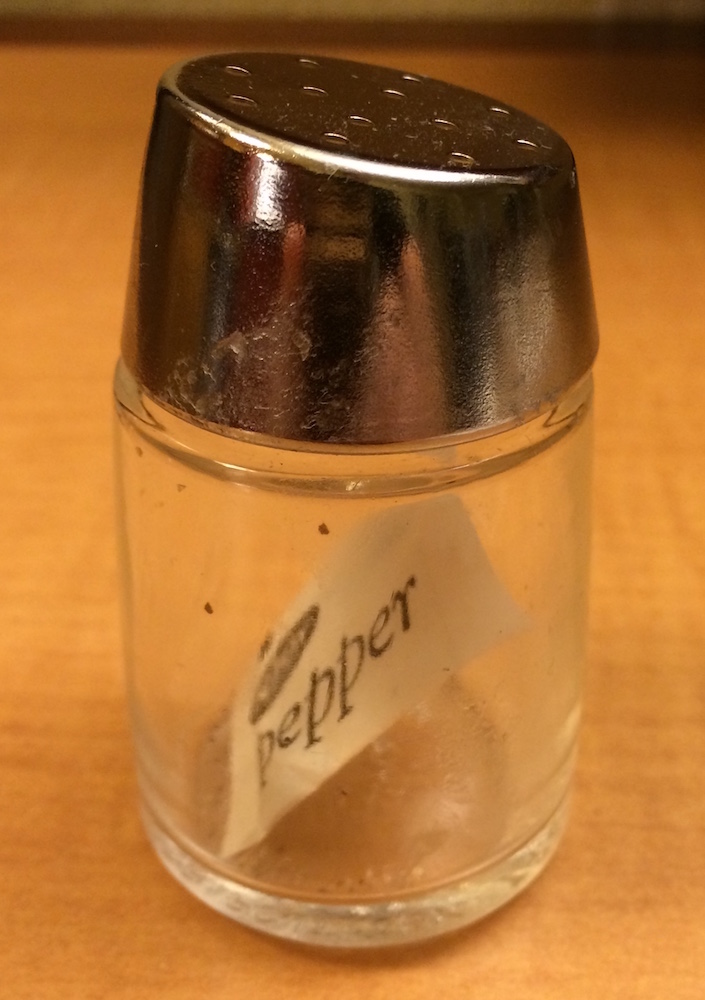
\includegraphics{images/pepper-1.jpg}\strut
\end{minipage}\tabularnewline
\begin{minipage}[t]{0.39\columnwidth}\centering\strut
1 pacote de pimenta\strut
\end{minipage} & \begin{minipage}[t]{0.22\columnwidth}\centering\strut
frasco{[}{[}1{]}{]}\strut
\end{minipage} & \begin{minipage}[t]{0.30\columnwidth}\centering\strut
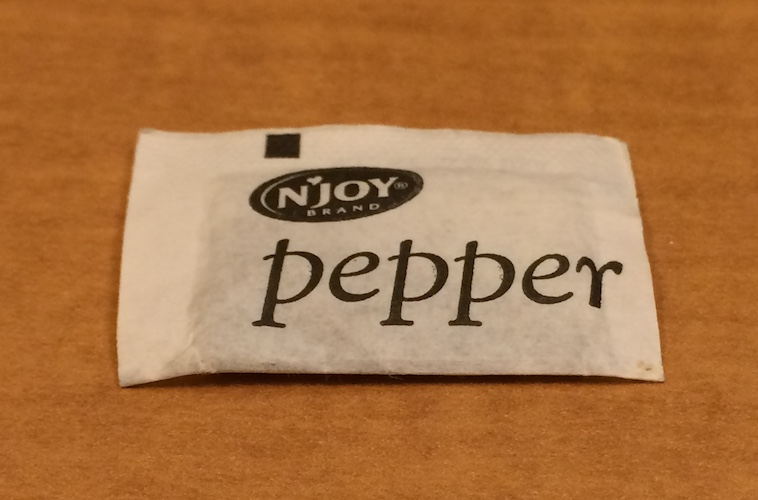
\includegraphics{images/pepper-2.jpg}\strut
\end{minipage}\tabularnewline
\begin{minipage}[t]{0.39\columnwidth}\centering\strut
conteúdo de um pacote de pimenta\strut
\end{minipage} & \begin{minipage}[t]{0.22\columnwidth}\centering\strut
frasco{[}{[}1{]}{]}{[}{[}1{]}{]}\strut
\end{minipage} & \begin{minipage}[t]{0.30\columnwidth}\centering\strut
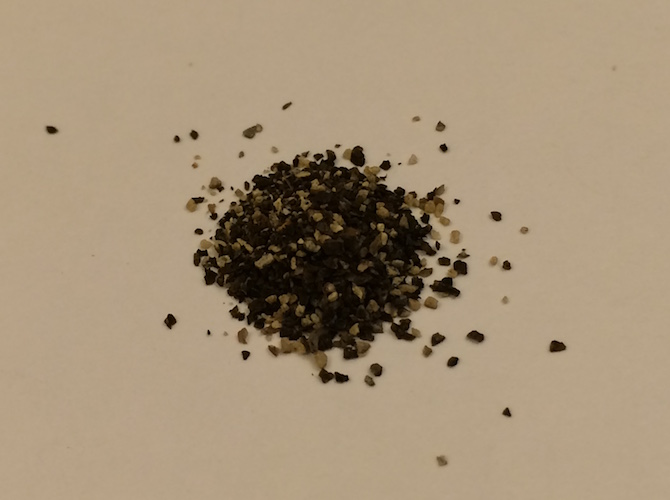
\includegraphics{images/pepper-3.jpg}\strut
\end{minipage}\tabularnewline
\bottomrule
\end{longtable}

\subsection{Conversão de lista para vetor e
vice-versa.}\label{conversao-de-lista-para-vetor-e-vice-versa.}

\begin{Shaded}
\begin{Highlighting}[]
\NormalTok{vet <-}\StringTok{ }\DecValTok{1}\OperatorTok{:}\DecValTok{10}
\NormalTok{vet}
\CommentTok{#>  [1]  1  2  3  4  5  6  7  8  9 10}
\NormalTok{vet.list <-}\StringTok{ }\KeywordTok{as.list}\NormalTok{(vet)}
\NormalTok{vet.list}
\CommentTok{#> [[1]]}
\CommentTok{#> [1] 1}
\CommentTok{#> }
\CommentTok{#> [[2]]}
\CommentTok{#> [1] 2}
\CommentTok{#> }
\CommentTok{#> [[3]]}
\CommentTok{#> [1] 3}
\CommentTok{#> }
\CommentTok{#> [[4]]}
\CommentTok{#> [1] 4}
\CommentTok{#> }
\CommentTok{#> [[5]]}
\CommentTok{#> [1] 5}
\CommentTok{#> }
\CommentTok{#> [[6]]}
\CommentTok{#> [1] 6}
\CommentTok{#> }
\CommentTok{#> [[7]]}
\CommentTok{#> [1] 7}
\CommentTok{#> }
\CommentTok{#> [[8]]}
\CommentTok{#> [1] 8}
\CommentTok{#> }
\CommentTok{#> [[9]]}
\CommentTok{#> [1] 9}
\CommentTok{#> }
\CommentTok{#> [[10]]}
\CommentTok{#> [1] 10}
\CommentTok{# desmanchando a lista}
\KeywordTok{unlist}\NormalTok{(vet.list)}
\CommentTok{#>  [1]  1  2  3  4  5  6  7  8  9 10}
\CommentTok{# deletando um elemento de uma lista}
\KeywordTok{length}\NormalTok{(vet.list)}
\CommentTok{#> [1] 10}
\NormalTok{vet.list[}\DecValTok{8}\NormalTok{] <-}\StringTok{ }\OtherTok{NULL}
\NormalTok{vet.list}
\CommentTok{#> [[1]]}
\CommentTok{#> [1] 1}
\CommentTok{#> }
\CommentTok{#> [[2]]}
\CommentTok{#> [1] 2}
\CommentTok{#> }
\CommentTok{#> [[3]]}
\CommentTok{#> [1] 3}
\CommentTok{#> }
\CommentTok{#> [[4]]}
\CommentTok{#> [1] 4}
\CommentTok{#> }
\CommentTok{#> [[5]]}
\CommentTok{#> [1] 5}
\CommentTok{#> }
\CommentTok{#> [[6]]}
\CommentTok{#> [1] 6}
\CommentTok{#> }
\CommentTok{#> [[7]]}
\CommentTok{#> [1] 7}
\CommentTok{#> }
\CommentTok{#> [[8]]}
\CommentTok{#> [1] 9}
\CommentTok{#> }
\CommentTok{#> [[9]]}
\CommentTok{#> [1] 10}
\KeywordTok{length}\NormalTok{(vet.list)}
\CommentTok{#> [1] 9}
\end{Highlighting}
\end{Shaded}

\subsection{\texorpdfstring{Conversão de \texttt{list} para
\texttt{data.frame}}{Conversão de list para data.frame}}\label{conversao-de-list-para-data.frame}

Vamos modificar a lista \texttt{sm\_l} para convertê-la em um
\emph{dataframe}.

\begin{Shaded}
\begin{Highlighting}[]
\NormalTok{sm_l}
\CommentTok{#> $coords}
\CommentTok{#> [1] -45 -23}
\CommentTok{#> }
\CommentTok{#> $cidade}
\CommentTok{#> [1] "Santa Maria"}
\CommentTok{#> }
\CommentTok{#> $dados}
\CommentTok{#>      tar prec}
\CommentTok{#> [1,]  31  300}
\CommentTok{#> [2,]  35  200}
\CommentTok{#> [3,]  21  150}
\CommentTok{#> [4,]  23  120}
\CommentTok{#> [5,]  33  210}
\CommentTok{#> [6,]  17  110}
\CommentTok{# ao invés da componente coords, criamos uma lon e lat}
\NormalTok{sm_l}\OperatorTok{$}\NormalTok{lon <-}\StringTok{ }\NormalTok{sm_l}\OperatorTok{$}\NormalTok{coords[}\DecValTok{1}\NormalTok{]}
\NormalTok{sm_l}\OperatorTok{$}\NormalTok{lat <-}\StringTok{ }\NormalTok{sm_l}\OperatorTok{$}\NormalTok{coords[}\DecValTok{2}\NormalTok{]}
\NormalTok{sm_l}\OperatorTok{$}\NormalTok{coords <-}\StringTok{ }\OtherTok{NULL}
\NormalTok{sm_l}
\CommentTok{#> $cidade}
\CommentTok{#> [1] "Santa Maria"}
\CommentTok{#> }
\CommentTok{#> $dados}
\CommentTok{#>      tar prec}
\CommentTok{#> [1,]  31  300}
\CommentTok{#> [2,]  35  200}
\CommentTok{#> [3,]  21  150}
\CommentTok{#> [4,]  23  120}
\CommentTok{#> [5,]  33  210}
\CommentTok{#> [6,]  17  110}
\CommentTok{#> }
\CommentTok{#> $lon}
\CommentTok{#> [1] -45}
\CommentTok{#> }
\CommentTok{#> $lat}
\CommentTok{#> [1] -23}
\CommentTok{# converter para dataframe}
\NormalTok{sm_df <-}\StringTok{ }\KeywordTok{data.frame}\NormalTok{(sm_l)}
\NormalTok{sm_df}
\CommentTok{#>        cidade dados.tar dados.prec lon lat}
\CommentTok{#> 1 Santa Maria        31        300 -45 -23}
\CommentTok{#> 2 Santa Maria        35        200 -45 -23}
\CommentTok{#> 3 Santa Maria        21        150 -45 -23}
\CommentTok{#> 4 Santa Maria        23        120 -45 -23}
\CommentTok{#> 5 Santa Maria        33        210 -45 -23}
\CommentTok{#> 6 Santa Maria        17        110 -45 -23}
\end{Highlighting}
\end{Shaded}

\section{Dataframe}\label{dataframe}

Um dataframe é o objeto mais usado para guardar conjunto de dados na
forma de tabela (tabulares ou planos).

A estrutura de um \emph{dataframe} é retangular como a de uma matriz.
Mas tem a vantagem de armazenar vetores de diferentes tipos
(\texttt{character}, \texttt{numeric}, \texttt{logical} e etc) nas suas
colunas. O que não é possível em uma matriz. Ou seja é uma estrutura de
armazenamento de dados heterogênea. \emph{Matrix}, \emph{arrays} e
\emph{vector} só armazenam dados homogêneos.

Cada linha do \emph{dataframe} corresponde a um registro da tabela. Cada
coluna corresponde a uma variável a ser armazenada para cada registro da
tabela.

\subsection{Criação}\label{criacao-3}

Uma das formas mais simples de se criar um \emph{dataframe} é através da
função \texttt{data.frame()}.

\begin{Shaded}
\begin{Highlighting}[]
\CommentTok{# criando um dataframe}
\NormalTok{dados <-}\StringTok{ }\KeywordTok{data.frame}\NormalTok{(}
  \DataTypeTok{datas =} \KeywordTok{c}\NormalTok{(}
    \StringTok{"2013-01-01"}\NormalTok{, }\StringTok{"2013-01-02"}\NormalTok{, }\StringTok{"2013-01-03"}\NormalTok{, }\StringTok{"2013-01-04"}\NormalTok{, }\StringTok{"2013-01-05"}\NormalTok{,}
    \StringTok{"2013-01-06"}\NormalTok{, }\StringTok{"2013-01-07"}\NormalTok{, }\StringTok{"2013-01-08"}\NormalTok{, }\StringTok{"2013-01-09"}\NormalTok{, }\StringTok{"2013-01-10"}\NormalTok{,}
    \StringTok{"2013-01-11"}\NormalTok{, }\StringTok{"2013-01-12"}\NormalTok{, }\StringTok{"2013-01-13"}\NormalTok{, }\StringTok{"2013-01-14"}\NormalTok{, }\StringTok{"2013-01-15"}
\NormalTok{  ),}
  \DataTypeTok{cidade =} \KeywordTok{rep}\NormalTok{(}\StringTok{"Santa Maria"}\NormalTok{, }\DecValTok{15}\NormalTok{),}
  \DataTypeTok{tar =} \KeywordTok{c}\NormalTok{(}\DecValTok{31}\NormalTok{, }\DecValTok{35}\NormalTok{, }\DecValTok{21}\NormalTok{, }\DecValTok{23}\NormalTok{, }\DecValTok{33}\NormalTok{, }\DecValTok{17}\NormalTok{, }\DecValTok{18}\NormalTok{, }\DecValTok{16}\NormalTok{, }\DecValTok{34}\NormalTok{, }\DecValTok{27}\NormalTok{, }\DecValTok{15}\NormalTok{, }\DecValTok{28}\NormalTok{, }\DecValTok{22}\NormalTok{, }\DecValTok{29}\NormalTok{, }\DecValTok{32}\NormalTok{)}
\NormalTok{)}
\NormalTok{dados}
\CommentTok{#>         datas      cidade tar}
\CommentTok{#> 1  2013-01-01 Santa Maria  31}
\CommentTok{#> 2  2013-01-02 Santa Maria  35}
\CommentTok{#> 3  2013-01-03 Santa Maria  21}
\CommentTok{#> 4  2013-01-04 Santa Maria  23}
\CommentTok{#> 5  2013-01-05 Santa Maria  33}
\CommentTok{#> 6  2013-01-06 Santa Maria  17}
\CommentTok{#> 7  2013-01-07 Santa Maria  18}
\CommentTok{#> 8  2013-01-08 Santa Maria  16}
\CommentTok{#> 9  2013-01-09 Santa Maria  34}
\CommentTok{#> 10 2013-01-10 Santa Maria  27}
\CommentTok{#> 11 2013-01-11 Santa Maria  15}
\CommentTok{#> 12 2013-01-12 Santa Maria  28}
\CommentTok{#> 13 2013-01-13 Santa Maria  22}
\CommentTok{#> 14 2013-01-14 Santa Maria  29}
\CommentTok{#> 15 2013-01-15 Santa Maria  32}
\KeywordTok{class}\NormalTok{(dados)}
\CommentTok{#> [1] "data.frame"}
\KeywordTok{is.data.frame}\NormalTok{(dados)}
\CommentTok{#> [1] TRUE}
\end{Highlighting}
\end{Shaded}

Para um diagnóstico rápido das variáveis de um \texttt{dataframe} usamos
a função \texttt{str()}:

\begin{Shaded}
\begin{Highlighting}[]
\CommentTok{# descrição geral do conjunto de dados}
\KeywordTok{str}\NormalTok{(dados)}
\CommentTok{#> 'data.frame':    15 obs. of  3 variables:}
\CommentTok{#>  $ datas : Factor w/ 15 levels "2013-01-01","2013-01-02",..: 1 2 3 4 5 6 7 8 9 10 ...}
\CommentTok{#>  $ cidade: Factor w/ 1 level "Santa Maria": 1 1 1 1 1 1 1 1 1 1 ...}
\CommentTok{#>  $ tar   : num  31 35 21 23 33 17 18 16 34 27 ...}
\end{Highlighting}
\end{Shaded}

A saída da função \texttt{str()}indica que há duas variáveis da classe
\texttt{factor}. Em um \emph{dataframe} vetores do tipo
\texttt{character} são automaticamente convertidos em \texttt{factor}.
Este é o comportamento \emph{default} da função \texttt{data.frame()}.
Para que essa conversão não seja feita você deve definir o parâmetro
\texttt{stringsAsFactors\ =\ FALSE} na função \texttt{data.frame()}.
Vamos recriar o \emph{dataframe} \texttt{dados} sem a conversão de
\texttt{character} para \texttt{factor}.

\begin{Shaded}
\begin{Highlighting}[]
\CommentTok{# criando um dataframe}
\NormalTok{dados <-}\StringTok{ }\KeywordTok{data.frame}\NormalTok{(}
  \DataTypeTok{datas =} \KeywordTok{c}\NormalTok{(}
    \StringTok{"2013-01-01"}\NormalTok{, }\StringTok{"2013-01-02"}\NormalTok{, }\StringTok{"2013-01-03"}\NormalTok{, }\StringTok{"2013-01-04"}\NormalTok{, }\StringTok{"2013-01-05"}\NormalTok{,}
    \StringTok{"2013-01-06"}\NormalTok{, }\StringTok{"2013-01-07"}\NormalTok{, }\StringTok{"2013-01-08"}\NormalTok{, }\StringTok{"2013-01-09"}\NormalTok{, }\StringTok{"2013-01-10"}\NormalTok{,}
    \StringTok{"2013-01-11"}\NormalTok{, }\StringTok{"2013-01-12"}\NormalTok{, }\StringTok{"2013-01-13"}\NormalTok{, }\StringTok{"2013-01-14"}\NormalTok{, }\StringTok{"2013-01-15"}
\NormalTok{  ),}
  \DataTypeTok{cidade =} \KeywordTok{rep}\NormalTok{(}\StringTok{"Santa Maria"}\NormalTok{, }\DecValTok{15}\NormalTok{),}
  \DataTypeTok{tar =} \KeywordTok{c}\NormalTok{(}\DecValTok{31}\NormalTok{, }\DecValTok{35}\NormalTok{, }\DecValTok{21}\NormalTok{, }\DecValTok{23}\NormalTok{, }\DecValTok{33}\NormalTok{, }\DecValTok{17}\NormalTok{, }\DecValTok{18}\NormalTok{, }\DecValTok{16}\NormalTok{, }\DecValTok{34}\NormalTok{, }\DecValTok{27}\NormalTok{, }\DecValTok{15}\NormalTok{, }\DecValTok{28}\NormalTok{, }\DecValTok{22}\NormalTok{, }\DecValTok{29}\NormalTok{, }\DecValTok{32}\NormalTok{),}
  \DataTypeTok{stringsAsFactors =} \OtherTok{FALSE}
\NormalTok{)}
\KeywordTok{str}\NormalTok{(dados)}
\CommentTok{#> 'data.frame':    15 obs. of  3 variables:}
\CommentTok{#>  $ datas : chr  "2013-01-01" "2013-01-02" "2013-01-03" "2013-01-04" ...}
\CommentTok{#>  $ cidade: chr  "Santa Maria" "Santa Maria" "Santa Maria" "Santa Maria" ...}
\CommentTok{#>  $ tar   : num  31 35 21 23 33 17 18 16 34 27 ...}
\end{Highlighting}
\end{Shaded}

A função \texttt{summary()} fornece um resumo estatístico das variáveis
(colunas) de um \emph{dataframe}.

\begin{Shaded}
\begin{Highlighting}[]
\CommentTok{# resumo estatístico dos dados}
\KeywordTok{summary}\NormalTok{(dados)}
\CommentTok{#>     datas              cidade               tar      }
\CommentTok{#>  Length:15          Length:15          Min.   :15.0  }
\CommentTok{#>  Class :character   Class :character   1st Qu.:19.5  }
\CommentTok{#>  Mode  :character   Mode  :character   Median :27.0  }
\CommentTok{#>                                        Mean   :25.4  }
\CommentTok{#>                                        3rd Qu.:31.5  }
\CommentTok{#>                                        Max.   :35.0}
\end{Highlighting}
\end{Shaded}

\subsection{\texorpdfstring{Atributos de um
\emph{dataframe}}{Atributos de um dataframe}}\label{atributos-de-um-dataframe}

\emph{dataframe} é uma estrutura de dados avançada e possui diversos
atributos.

\begin{Shaded}
\begin{Highlighting}[]
\CommentTok{# atributos}
\KeywordTok{attributes}\NormalTok{(dados)}
\CommentTok{#> $names}
\CommentTok{#> [1] "datas"  "cidade" "tar"   }
\CommentTok{#> }
\CommentTok{#> $row.names}
\CommentTok{#>  [1]  1  2  3  4  5  6  7  8  9 10 11 12 13 14 15}
\CommentTok{#> }
\CommentTok{#> $class}
\CommentTok{#> [1] "data.frame"}
\CommentTok{# atributos armazenados em uma lista}
\KeywordTok{str}\NormalTok{(}\KeywordTok{attributes}\NormalTok{(dados))}
\CommentTok{#> List of 3}
\CommentTok{#>  $ names    : chr [1:3] "datas" "cidade" "tar"}
\CommentTok{#>  $ row.names: int [1:15] 1 2 3 4 5 6 7 8 9 10 ...}
\CommentTok{#>  $ class    : chr "data.frame"}
\CommentTok{# número de colunas}
\KeywordTok{ncol}\NormalTok{(dados)}
\CommentTok{#> [1] 3}
\CommentTok{# número de linhas}
\KeywordTok{nrow}\NormalTok{(dados)}
\CommentTok{#> [1] 15}
\CommentTok{# dimensões}
\KeywordTok{dim}\NormalTok{(dados)}
\CommentTok{#> [1] 15  3}
\CommentTok{# nomes podem ser atribuídos as linhas e as colunas}
\KeywordTok{rownames}\NormalTok{(dados)}
\CommentTok{#>  [1] "1"  "2"  "3"  "4"  "5"  "6"  "7"  "8"  "9"  "10" "11" "12" "13" "14"}
\CommentTok{#> [15] "15"}
\CommentTok{# novos nomes para as linhas de dados}
\KeywordTok{rownames}\NormalTok{(dados) <-}\StringTok{ }\KeywordTok{paste0}\NormalTok{(}\StringTok{"linha"}\NormalTok{, }\KeywordTok{rownames}\NormalTok{(dados))}
\NormalTok{dados}
\CommentTok{#>              datas      cidade tar}
\CommentTok{#> linha1  2013-01-01 Santa Maria  31}
\CommentTok{#> linha2  2013-01-02 Santa Maria  35}
\CommentTok{#> linha3  2013-01-03 Santa Maria  21}
\CommentTok{#> linha4  2013-01-04 Santa Maria  23}
\CommentTok{#> linha5  2013-01-05 Santa Maria  33}
\CommentTok{#> linha6  2013-01-06 Santa Maria  17}
\CommentTok{#> linha7  2013-01-07 Santa Maria  18}
\CommentTok{#> linha8  2013-01-08 Santa Maria  16}
\CommentTok{#> linha9  2013-01-09 Santa Maria  34}
\CommentTok{#> linha10 2013-01-10 Santa Maria  27}
\CommentTok{#> linha11 2013-01-11 Santa Maria  15}
\CommentTok{#> linha12 2013-01-12 Santa Maria  28}
\CommentTok{#> linha13 2013-01-13 Santa Maria  22}
\CommentTok{#> linha14 2013-01-14 Santa Maria  29}
\CommentTok{#> linha15 2013-01-15 Santa Maria  32}
\CommentTok{# removendo nomes das linhas}
\KeywordTok{rownames}\NormalTok{(dados) <-}\StringTok{ }\OtherTok{NULL}
\NormalTok{dados}
\CommentTok{#>         datas      cidade tar}
\CommentTok{#> 1  2013-01-01 Santa Maria  31}
\CommentTok{#> 2  2013-01-02 Santa Maria  35}
\CommentTok{#> 3  2013-01-03 Santa Maria  21}
\CommentTok{#> 4  2013-01-04 Santa Maria  23}
\CommentTok{#> 5  2013-01-05 Santa Maria  33}
\CommentTok{#> 6  2013-01-06 Santa Maria  17}
\CommentTok{#> 7  2013-01-07 Santa Maria  18}
\CommentTok{#> 8  2013-01-08 Santa Maria  16}
\CommentTok{#> 9  2013-01-09 Santa Maria  34}
\CommentTok{#> 10 2013-01-10 Santa Maria  27}
\CommentTok{#> 11 2013-01-11 Santa Maria  15}
\CommentTok{#> 12 2013-01-12 Santa Maria  28}
\CommentTok{#> 13 2013-01-13 Santa Maria  22}
\CommentTok{#> 14 2013-01-14 Santa Maria  29}
\CommentTok{#> 15 2013-01-15 Santa Maria  32}
\CommentTok{# mesmo que names(dados)}
\KeywordTok{colnames}\NormalTok{(dados)}
\CommentTok{#> [1] "datas"  "cidade" "tar"}
\CommentTok{# ou simplesmente}
\KeywordTok{names}\NormalTok{(dados)}
\CommentTok{#> [1] "datas"  "cidade" "tar"}
\end{Highlighting}
\end{Shaded}

\subsection{\texorpdfstring{Acesso as variáveis de um
\emph{dataframe}}{Acesso as variáveis de um dataframe}}\label{acesso-as-variaveis-de-um-dataframe}

Existem várias formas de acessar as variáveis de um \emph{dataframe}. Os
operadores para extração de elementos são os mesmos utilizados para
extração de elementos de uma lista: \texttt{{[}}, \texttt{{[}{[}} e
\texttt{\$}. Mas observe a diferença nos resultados extraídos com cada
operador.

\begin{Shaded}
\begin{Highlighting}[]
\CommentTok{# variáveis do dataframe}
\KeywordTok{names}\NormalTok{(dados)}
\CommentTok{#> [1] "datas"  "cidade" "tar"}
\CommentTok{# acessando os dados de temperatura}
\NormalTok{dados[, }\DecValTok{3}\NormalTok{]}
\CommentTok{#>  [1] 31 35 21 23 33 17 18 16 34 27 15 28 22 29 32}
\CommentTok{# ou}
\NormalTok{dados[, }\StringTok{"tar"}\NormalTok{]}
\CommentTok{#>  [1] 31 35 21 23 33 17 18 16 34 27 15 28 22 29 32}
\CommentTok{# ou}
\NormalTok{dados}\OperatorTok{$}\NormalTok{tar}
\CommentTok{#>  [1] 31 35 21 23 33 17 18 16 34 27 15 28 22 29 32}
\KeywordTok{is.vector}\NormalTok{(dados}\OperatorTok{$}\NormalTok{tar)}
\CommentTok{#> [1] TRUE}
\CommentTok{# note a diferença no resultado da extração}
\NormalTok{dados[}\StringTok{"tar"}\NormalTok{]}
\CommentTok{#>    tar}
\CommentTok{#> 1   31}
\CommentTok{#> 2   35}
\CommentTok{#> 3   21}
\CommentTok{#> 4   23}
\CommentTok{#> 5   33}
\CommentTok{#> 6   17}
\CommentTok{#> 7   18}
\CommentTok{#> 8   16}
\CommentTok{#> 9   34}
\CommentTok{#> 10  27}
\CommentTok{#> 11  15}
\CommentTok{#> 12  28}
\CommentTok{#> 13  22}
\CommentTok{#> 14  29}
\CommentTok{#> 15  32}
\KeywordTok{class}\NormalTok{(dados[}\StringTok{"tar"}\NormalTok{])}
\CommentTok{#> [1] "data.frame"}
\NormalTok{dados[[}\StringTok{"tar"}\NormalTok{]]}
\CommentTok{#>  [1] 31 35 21 23 33 17 18 16 34 27 15 28 22 29 32}
\KeywordTok{class}\NormalTok{(dados[[}\StringTok{"tar"}\NormalTok{]])}
\CommentTok{#> [1] "numeric"}
\NormalTok{dados[, }\StringTok{"tar"}\NormalTok{]}
\CommentTok{#>  [1] 31 35 21 23 33 17 18 16 34 27 15 28 22 29 32}
\KeywordTok{class}\NormalTok{(dados[, }\StringTok{"tar"}\NormalTok{])}
\CommentTok{#> [1] "numeric"}
\end{Highlighting}
\end{Shaded}

Portanto \emph{dataframes} tem estrutura retangular similar a das
matrizes e algumas de listas (diferentes colunas podem conter diferentes
tipos de objetos).

\subsubsection{\texorpdfstring{Função
\texttt{with()}}{Função with()}}\label{funcao-with}

O acesso as variáveis de um \emph{dataframe} também é possível com a
função \texttt{with(data,\ expr)}.

\begin{Shaded}
\begin{Highlighting}[]
\CommentTok{# acesso a variáveis de um dataframe}
\KeywordTok{with}\NormalTok{(}\DataTypeTok{data =}\NormalTok{ dados, }\DataTypeTok{expr =}\NormalTok{ tar)}
\CommentTok{#>  [1] 31 35 21 23 33 17 18 16 34 27 15 28 22 29 32}
\NormalTok{tarK <-}\StringTok{ }\KeywordTok{with}\NormalTok{(}\DataTypeTok{data =}\NormalTok{ dados, }\DataTypeTok{expr =}\NormalTok{ tar }\OperatorTok{+}\StringTok{ }\FloatTok{273.15}\NormalTok{)}
\NormalTok{tarK}
\CommentTok{#>  [1] 304.15 308.15 294.15 296.15 306.15 290.15 291.15 289.15 307.15 300.15}
\CommentTok{#> [11] 288.15 301.15 295.15 302.15 305.15}
\KeywordTok{with}\NormalTok{(}\DataTypeTok{data =}\NormalTok{ dados, }
     \CommentTok{# parâmetro expr geralmente não é mostrado}
       \KeywordTok{plot}\NormalTok{(tar }\OperatorTok{+}\StringTok{ }\FloatTok{273.15}\NormalTok{, }\DataTypeTok{type =} \StringTok{"o"}\NormalTok{)}
\NormalTok{     )}
\end{Highlighting}
\end{Shaded}

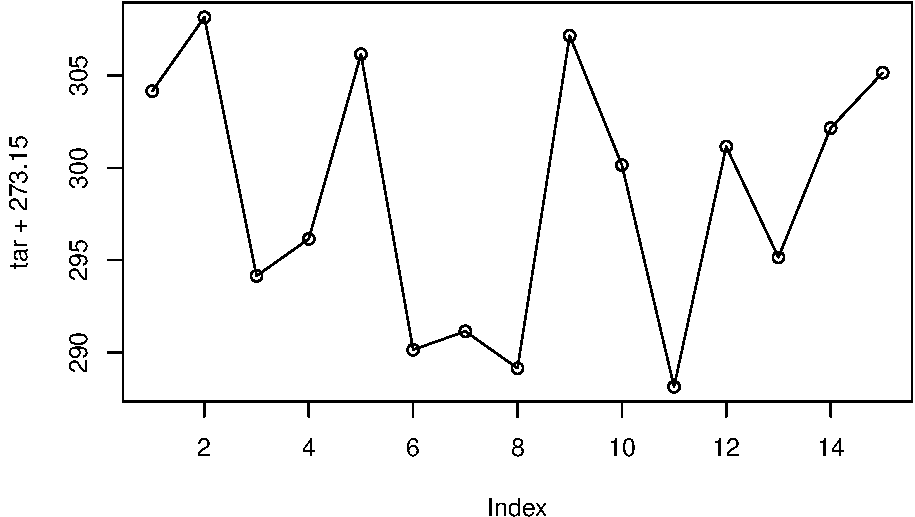
\includegraphics{images/Chunk5310-1.pdf}

O argumento pode ser substituído por qualquer expressão ou conjunto de
expressões que envolvam as variáveis do \emph{dataframe} de entrada.

\begin{Shaded}
\begin{Highlighting}[]
\KeywordTok{with}\NormalTok{(dados,\{}
  \KeywordTok{plot}\NormalTok{(}\KeywordTok{as.Date}\NormalTok{(datas), tar)}
\NormalTok{\})}
\end{Highlighting}
\end{Shaded}

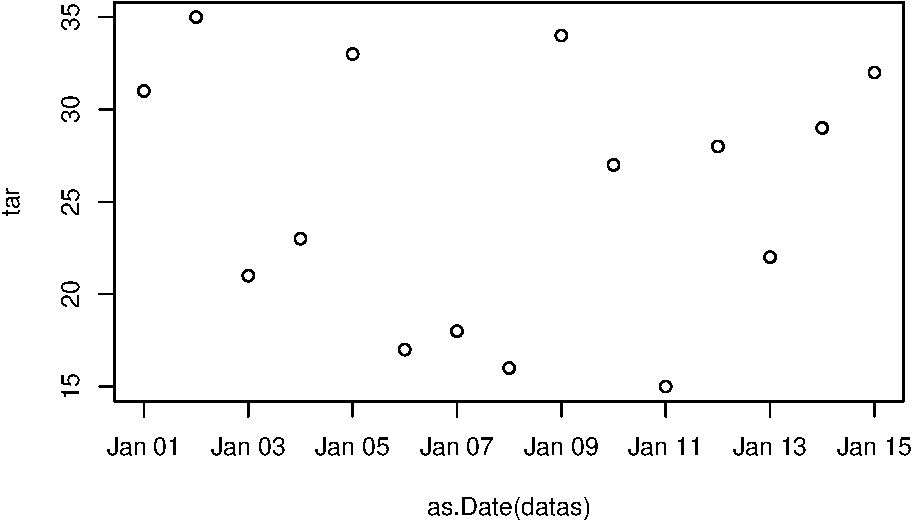
\includegraphics{images/unnamed-chunk-5-1.pdf}

\subsubsection{\texorpdfstring{Edição manual de um
\emph{dataframe}}{Edição manual de um dataframe}}\label{edicao-manual-de-um-dataframe}

É possível também editar os dados manualmente.

\begin{Shaded}
\begin{Highlighting}[]
\CommentTok{# editar dados}
\KeywordTok{fix}\NormalTok{(dados)}
\CommentTok{# inicializando um dataframe}
\NormalTok{x <-}\StringTok{ }\KeywordTok{data.frame}\NormalTok{()}
\CommentTok{# digitando so dados}
\KeywordTok{fix}\NormalTok{(x)}
\end{Highlighting}
\end{Shaded}

\subsection{Indexação, seleção e
alteração}\label{indexacao-selecao-e-alteracao}

Todos esquemas de indexação usados para matrizes (seleção por índices,
nomes, vetores lógicos - \emph{ver Aula9}) podem ser usados com
\emph{dataframes}.

\begin{Shaded}
\begin{Highlighting}[]
\CommentTok{# todos dados exceto o primeiro e último registro}
\NormalTok{dados[}\OperatorTok{-}\KeywordTok{c}\NormalTok{(}\DecValTok{1}\NormalTok{, }\KeywordTok{nrow}\NormalTok{(dados)), ]}
\CommentTok{#>         datas      cidade tar}
\CommentTok{#> 2  2013-01-02 Santa Maria  35}
\CommentTok{#> 3  2013-01-03 Santa Maria  21}
\CommentTok{#> 4  2013-01-04 Santa Maria  23}
\CommentTok{#> 5  2013-01-05 Santa Maria  33}
\CommentTok{#> 6  2013-01-06 Santa Maria  17}
\CommentTok{#> 7  2013-01-07 Santa Maria  18}
\CommentTok{#> 8  2013-01-08 Santa Maria  16}
\CommentTok{#> 9  2013-01-09 Santa Maria  34}
\CommentTok{#> 10 2013-01-10 Santa Maria  27}
\CommentTok{#> 11 2013-01-11 Santa Maria  15}
\CommentTok{#> 12 2013-01-12 Santa Maria  28}
\CommentTok{#> 13 2013-01-13 Santa Maria  22}
\CommentTok{#> 14 2013-01-14 Santa Maria  29}
\CommentTok{# temperatura dos primeiros 5 dias}
\NormalTok{dados[}\DecValTok{1}\OperatorTok{:}\DecValTok{5}\NormalTok{, }\DecValTok{3}\NormalTok{]}
\CommentTok{#> [1] 31 35 21 23 33}
\CommentTok{# temperatura no dia 2013-01-09}
\NormalTok{dados[dados}\OperatorTok{$}\NormalTok{datas }\OperatorTok{==}\StringTok{ "2013-01-09"}\NormalTok{, }\StringTok{"tar"}\NormalTok{]}
\CommentTok{#> [1] 34}
\CommentTok{# acrescentar uma nova variavel}
\NormalTok{dados}\OperatorTok{$}\NormalTok{prec <-}\StringTok{ }\KeywordTok{c}\NormalTok{(}\KeywordTok{rep}\NormalTok{(}\DecValTok{0}\NormalTok{, }\DecValTok{5}\NormalTok{), }\DecValTok{10}\NormalTok{, }\DecValTok{18}\NormalTok{, }\DecValTok{4}\NormalTok{, }\DecValTok{0}\NormalTok{, }\DecValTok{0}\NormalTok{, }\DecValTok{5}\NormalTok{, }\DecValTok{0}\NormalTok{, }\DecValTok{0}\NormalTok{, }\DecValTok{2}\NormalTok{, }\DecValTok{0}\NormalTok{)}
\NormalTok{dados}
\CommentTok{#>         datas      cidade tar prec}
\CommentTok{#> 1  2013-01-01 Santa Maria  31    0}
\CommentTok{#> 2  2013-01-02 Santa Maria  35    0}
\CommentTok{#> 3  2013-01-03 Santa Maria  21    0}
\CommentTok{#> 4  2013-01-04 Santa Maria  23    0}
\CommentTok{#> 5  2013-01-05 Santa Maria  33    0}
\CommentTok{#> 6  2013-01-06 Santa Maria  17   10}
\CommentTok{#> 7  2013-01-07 Santa Maria  18   18}
\CommentTok{#> 8  2013-01-08 Santa Maria  16    4}
\CommentTok{#> 9  2013-01-09 Santa Maria  34    0}
\CommentTok{#> 10 2013-01-10 Santa Maria  27    0}
\CommentTok{#> 11 2013-01-11 Santa Maria  15    5}
\CommentTok{#> 12 2013-01-12 Santa Maria  28    0}
\CommentTok{#> 13 2013-01-13 Santa Maria  22    0}
\CommentTok{#> 14 2013-01-14 Santa Maria  29    2}
\CommentTok{#> 15 2013-01-15 Santa Maria  32    0}
\end{Highlighting}
\end{Shaded}

Uma função específica para gerar subconjunto de dados em
\emph{dataframes} é a \texttt{subset()}.

\begin{Shaded}
\begin{Highlighting}[]
\CommentTok{# subconjunto baseado em condição lógica}
\NormalTok{ss1 <-}\StringTok{ }\KeywordTok{subset}\NormalTok{(dados, datas }\OperatorTok{==}\StringTok{ "2013-01-09"}\NormalTok{, }\DataTypeTok{select =} \StringTok{"tar"}\NormalTok{)}
\NormalTok{ss1}
\CommentTok{#>   tar}
\CommentTok{#> 9  34}
\CommentTok{# subconjunto baseado em condição lógica}
\NormalTok{ss2 <-}\StringTok{ }\KeywordTok{subset}\NormalTok{(dados, tar }\OperatorTok{>}\StringTok{ }\DecValTok{26} \OperatorTok{&}\StringTok{ }\NormalTok{prec }\OperatorTok{>}\StringTok{ }\DecValTok{0}\NormalTok{)}
\NormalTok{ss2}
\CommentTok{#>         datas      cidade tar prec}
\CommentTok{#> 14 2013-01-14 Santa Maria  29    2}
\CommentTok{# subconjunto baseado em condição lógica}
\NormalTok{ss3 <-}\StringTok{ }\KeywordTok{subset}\NormalTok{(dados, tar }\OperatorTok{>}\StringTok{ }\DecValTok{26} \OperatorTok{|}\StringTok{ }\NormalTok{prec }\OperatorTok{>}\StringTok{ }\DecValTok{0}\NormalTok{)}
\NormalTok{ss3}
\CommentTok{#>         datas      cidade tar prec}
\CommentTok{#> 1  2013-01-01 Santa Maria  31    0}
\CommentTok{#> 2  2013-01-02 Santa Maria  35    0}
\CommentTok{#> 5  2013-01-05 Santa Maria  33    0}
\CommentTok{#> 6  2013-01-06 Santa Maria  17   10}
\CommentTok{#> 7  2013-01-07 Santa Maria  18   18}
\CommentTok{#> 8  2013-01-08 Santa Maria  16    4}
\CommentTok{#> 9  2013-01-09 Santa Maria  34    0}
\CommentTok{#> 10 2013-01-10 Santa Maria  27    0}
\CommentTok{#> 11 2013-01-11 Santa Maria  15    5}
\CommentTok{#> 12 2013-01-12 Santa Maria  28    0}
\CommentTok{#> 14 2013-01-14 Santa Maria  29    2}
\CommentTok{#> 15 2013-01-15 Santa Maria  32    0}
\CommentTok{# subconjunto baseado em condição lógica}
\NormalTok{ss4 <-}\StringTok{ }\KeywordTok{subset}\NormalTok{(dados,}
\NormalTok{  datas }\OperatorTok\StringTok{ }\KeywordTok{c}\NormalTok{(}\StringTok{"2013-01-09"}\NormalTok{, }\StringTok{"2013-01-13"}\NormalTok{, }\StringTok{"2013-01-15"}\NormalTok{),}
  \DataTypeTok{select =} \OperatorTok{-}\NormalTok{cidade}
\NormalTok{)}
\NormalTok{ss4}
\CommentTok{#>         datas tar prec}
\CommentTok{#> 9  2013-01-09  34    0}
\CommentTok{#> 13 2013-01-13  22    0}
\CommentTok{#> 15 2013-01-15  32    0}
\CommentTok{# subconjunto baseado em condição lógica}
\NormalTok{ss4 <-}\StringTok{ }\KeywordTok{subset}\NormalTok{(dados,}
  \OperatorTok{!}\NormalTok{datas }\OperatorTok\StringTok{ }\KeywordTok{c}\NormalTok{(}\StringTok{"2013-01-09"}\NormalTok{, }\StringTok{"2013-01-13"}\NormalTok{, }\StringTok{"2013-01-15"}\NormalTok{),}
  \DataTypeTok{select =} \OperatorTok{-}\NormalTok{cidade}
\NormalTok{)}
\NormalTok{ss4}
\CommentTok{#>         datas tar prec}
\CommentTok{#> 1  2013-01-01  31    0}
\CommentTok{#> 2  2013-01-02  35    0}
\CommentTok{#> 3  2013-01-03  21    0}
\CommentTok{#> 4  2013-01-04  23    0}
\CommentTok{#> 5  2013-01-05  33    0}
\CommentTok{#> 6  2013-01-06  17   10}
\CommentTok{#> 7  2013-01-07  18   18}
\CommentTok{#> 8  2013-01-08  16    4}
\CommentTok{#> 10 2013-01-10  27    0}
\CommentTok{#> 11 2013-01-11  15    5}
\CommentTok{#> 12 2013-01-12  28    0}
\CommentTok{#> 14 2013-01-14  29    2}
\end{Highlighting}
\end{Shaded}

Uma função específica para alteração, remoção e inclusão de variáveis em
um \emph{dataframe} é a \texttt{transform()}. Essa função é mais
indicada para alteração de mais de uma variável de um \emph{dataframe}.

\begin{Shaded}
\begin{Highlighting}[]
\CommentTok{# mudança do dataframe, alteração de várias variáveis}
\NormalTok{dados <-}\StringTok{ }\KeywordTok{transform}\NormalTok{(dados,}
  \DataTypeTok{cidade =} \KeywordTok{ifelse}\NormalTok{(}\DecValTok{1}\OperatorTok{:}\KeywordTok{nrow}\NormalTok{(dados) }\OperatorTok{>}\StringTok{ }\DecValTok{8}\NormalTok{, }\StringTok{"Sao Sepe"}\NormalTok{, cidade),}
  \DataTypeTok{datas =} \KeywordTok{c}\NormalTok{(datas[}\DecValTok{1}\OperatorTok{:}\DecValTok{8}\NormalTok{], datas[}\DecValTok{1}\OperatorTok{:}\DecValTok{7}\NormalTok{]),}
  \DataTypeTok{anomalias =} \KeywordTok{ifelse}\NormalTok{(cidade }\OperatorTok{==}\StringTok{ "Santa Maria"}\NormalTok{,}
\NormalTok{    tar }\OperatorTok{-}\StringTok{ }\KeywordTok{mean}\NormalTok{(tar[cidade }\OperatorTok{==}\StringTok{ "Santa Maria"}\NormalTok{]),}
\NormalTok{    tar }\OperatorTok{-}\StringTok{ }\KeywordTok{mean}\NormalTok{(tar[cidade }\OperatorTok{==}\StringTok{ "Sao Sepe"}\NormalTok{])}
\NormalTok{  )}
\NormalTok{)}
\CommentTok{# alterar so uma variavel}
\NormalTok{dados}\OperatorTok{$}\NormalTok{anomalias.norm <-}\StringTok{ }\KeywordTok{ifelse}\NormalTok{(dados}\OperatorTok{$}\NormalTok{cidade }\OperatorTok{==}\StringTok{ "Santa Maria"}\NormalTok{,}
\NormalTok{  dados}\OperatorTok{$}\NormalTok{anomalias }\OperatorTok{/}\StringTok{ }\KeywordTok{sd}\NormalTok{(dados}\OperatorTok{$}\NormalTok{anomalias[dados}\OperatorTok{$}\NormalTok{cidade }\OperatorTok{==}\StringTok{ "Santa Maria"}\NormalTok{]),}
\NormalTok{  dados}\OperatorTok{$}\NormalTok{anomalias }\OperatorTok{/}\StringTok{ }\KeywordTok{sd}\NormalTok{(dados}\OperatorTok{$}\NormalTok{anomalias[dados}\OperatorTok{$}\NormalTok{cidade }\OperatorTok{==}\StringTok{ "Sao Sepe"}\NormalTok{])}
\NormalTok{)}
\NormalTok{dados}
\CommentTok{#>         datas      cidade tar prec anomalias anomalias.norm}
\CommentTok{#> 1  2013-01-01 Santa Maria  31    0       5.6       0.732167}
\CommentTok{#> 2  2013-01-02 Santa Maria  35    0       9.6       1.255143}
\CommentTok{#> 3  2013-01-03 Santa Maria  21    0      -4.4      -0.575274}
\CommentTok{#> 4  2013-01-04 Santa Maria  23    0      -2.4      -0.313786}
\CommentTok{#> 5  2013-01-05 Santa Maria  33    0       7.6       0.993655}
\CommentTok{#> 6  2013-01-06 Santa Maria  17   10      -8.4      -1.098250}
\CommentTok{#> 7  2013-01-07 Santa Maria  18   18      -7.4      -0.967506}
\CommentTok{#> 8  2013-01-08 Santa Maria  16    4      -9.4      -1.228994}
\CommentTok{#> 9  2013-01-01    Sao Sepe  34    0       8.6       1.339211}
\CommentTok{#> 10 2013-01-02    Sao Sepe  27    0       1.6       0.249156}
\CommentTok{#> 11 2013-01-03    Sao Sepe  15    5     -10.4      -1.619512}
\CommentTok{#> 12 2013-01-04    Sao Sepe  28    0       2.6       0.404878}
\CommentTok{#> 13 2013-01-05    Sao Sepe  22    0      -3.4      -0.529456}
\CommentTok{#> 14 2013-01-06    Sao Sepe  29    2       3.6       0.560600}
\CommentTok{#> 15 2013-01-07    Sao Sepe  32    0       6.6       1.027767}
\end{Highlighting}
\end{Shaded}

\subsection{\texorpdfstring{Combinando
\emph{dataframes}}{Combinando dataframes}}\label{combinando-dataframes}

\begin{Shaded}
\begin{Highlighting}[]
\NormalTok{coords.df <-}\StringTok{ }\KeywordTok{data.frame}\NormalTok{(}
  \DataTypeTok{lon =} \KeywordTok{c}\NormalTok{(}\KeywordTok{rep}\NormalTok{(}\OperatorTok{-}\DecValTok{45}\NormalTok{, }\DecValTok{8}\NormalTok{), }\KeywordTok{rep}\NormalTok{(}\OperatorTok{-}\FloatTok{45.1}\NormalTok{, }\DecValTok{7}\NormalTok{)), }\CommentTok{# longitudes}
  \DataTypeTok{lat =} \KeywordTok{c}\NormalTok{(}\KeywordTok{rep}\NormalTok{(}\OperatorTok{-}\DecValTok{23}\NormalTok{, }\DecValTok{8}\NormalTok{), }\KeywordTok{rep}\NormalTok{(}\OperatorTok{-}\FloatTok{23.1}\NormalTok{, }\DecValTok{7}\NormalTok{))}
\NormalTok{) }\CommentTok{# latitudes}
\NormalTok{d <-}\StringTok{ }\KeywordTok{cbind}\NormalTok{(dados, coords.df)}
\NormalTok{d}
\CommentTok{#>         datas      cidade tar prec anomalias anomalias.norm   lon   lat}
\CommentTok{#> 1  2013-01-01 Santa Maria  31    0       5.6       0.732167 -45.0 -23.0}
\CommentTok{#> 2  2013-01-02 Santa Maria  35    0       9.6       1.255143 -45.0 -23.0}
\CommentTok{#> 3  2013-01-03 Santa Maria  21    0      -4.4      -0.575274 -45.0 -23.0}
\CommentTok{#> 4  2013-01-04 Santa Maria  23    0      -2.4      -0.313786 -45.0 -23.0}
\CommentTok{#> 5  2013-01-05 Santa Maria  33    0       7.6       0.993655 -45.0 -23.0}
\CommentTok{#> 6  2013-01-06 Santa Maria  17   10      -8.4      -1.098250 -45.0 -23.0}
\CommentTok{#> 7  2013-01-07 Santa Maria  18   18      -7.4      -0.967506 -45.0 -23.0}
\CommentTok{#> 8  2013-01-08 Santa Maria  16    4      -9.4      -1.228994 -45.0 -23.0}
\CommentTok{#> 9  2013-01-01    Sao Sepe  34    0       8.6       1.339211 -45.1 -23.1}
\CommentTok{#> 10 2013-01-02    Sao Sepe  27    0       1.6       0.249156 -45.1 -23.1}
\CommentTok{#> 11 2013-01-03    Sao Sepe  15    5     -10.4      -1.619512 -45.1 -23.1}
\CommentTok{#> 12 2013-01-04    Sao Sepe  28    0       2.6       0.404878 -45.1 -23.1}
\CommentTok{#> 13 2013-01-05    Sao Sepe  22    0      -3.4      -0.529456 -45.1 -23.1}
\CommentTok{#> 14 2013-01-06    Sao Sepe  29    2       3.6       0.560600 -45.1 -23.1}
\CommentTok{#> 15 2013-01-07    Sao Sepe  32    0       6.6       1.027767 -45.1 -23.1}
\CommentTok{# usando a própria função data.frame()}
\NormalTok{d2 <-}\StringTok{ }\KeywordTok{data.frame}\NormalTok{(dados, coords.df, }\DataTypeTok{stringsAsFactors =} \OtherTok{FALSE}\NormalTok{)}
\NormalTok{d2}
\CommentTok{#>         datas      cidade tar prec anomalias anomalias.norm   lon   lat}
\CommentTok{#> 1  2013-01-01 Santa Maria  31    0       5.6       0.732167 -45.0 -23.0}
\CommentTok{#> 2  2013-01-02 Santa Maria  35    0       9.6       1.255143 -45.0 -23.0}
\CommentTok{#> 3  2013-01-03 Santa Maria  21    0      -4.4      -0.575274 -45.0 -23.0}
\CommentTok{#> 4  2013-01-04 Santa Maria  23    0      -2.4      -0.313786 -45.0 -23.0}
\CommentTok{#> 5  2013-01-05 Santa Maria  33    0       7.6       0.993655 -45.0 -23.0}
\CommentTok{#> 6  2013-01-06 Santa Maria  17   10      -8.4      -1.098250 -45.0 -23.0}
\CommentTok{#> 7  2013-01-07 Santa Maria  18   18      -7.4      -0.967506 -45.0 -23.0}
\CommentTok{#> 8  2013-01-08 Santa Maria  16    4      -9.4      -1.228994 -45.0 -23.0}
\CommentTok{#> 9  2013-01-01    Sao Sepe  34    0       8.6       1.339211 -45.1 -23.1}
\CommentTok{#> 10 2013-01-02    Sao Sepe  27    0       1.6       0.249156 -45.1 -23.1}
\CommentTok{#> 11 2013-01-03    Sao Sepe  15    5     -10.4      -1.619512 -45.1 -23.1}
\CommentTok{#> 12 2013-01-04    Sao Sepe  28    0       2.6       0.404878 -45.1 -23.1}
\CommentTok{#> 13 2013-01-05    Sao Sepe  22    0      -3.4      -0.529456 -45.1 -23.1}
\CommentTok{#> 14 2013-01-06    Sao Sepe  29    2       3.6       0.560600 -45.1 -23.1}
\CommentTok{#> 15 2013-01-07    Sao Sepe  32    0       6.6       1.027767 -45.1 -23.1}
\CommentTok{# verificando se os dois dataframes são idênticos}
\KeywordTok{identical}\NormalTok{(d, d2)}
\CommentTok{#> [1] TRUE}
\CommentTok{# dados de Caçapava}
\NormalTok{cacapava <-}\StringTok{ }\KeywordTok{data.frame}\NormalTok{(}
  \DataTypeTok{datas =} \StringTok{"2013-01-01"}\NormalTok{,}
  \DataTypeTok{cidade =} \StringTok{"Cacapava"}\NormalTok{,}
  \DataTypeTok{tar =} \DecValTok{19}\NormalTok{,}
  \DataTypeTok{prec =} \DecValTok{0}\NormalTok{,}
  \DataTypeTok{anomalias =} \OtherTok{NA}\NormalTok{,}
  \DataTypeTok{anomalias.norm =} \OtherTok{NA}\NormalTok{,}
  \DataTypeTok{lon =} \OperatorTok{-}\FloatTok{45.1}\NormalTok{,}
  \DataTypeTok{lat =} \OperatorTok{-}\FloatTok{23.2}
\NormalTok{)}
\NormalTok{d <-}\StringTok{ }\KeywordTok{rbind}\NormalTok{(d, cacapava)}
\NormalTok{d}
\CommentTok{#>         datas      cidade tar prec anomalias anomalias.norm   lon   lat}
\CommentTok{#> 1  2013-01-01 Santa Maria  31    0       5.6       0.732167 -45.0 -23.0}
\CommentTok{#> 2  2013-01-02 Santa Maria  35    0       9.6       1.255143 -45.0 -23.0}
\CommentTok{#> 3  2013-01-03 Santa Maria  21    0      -4.4      -0.575274 -45.0 -23.0}
\CommentTok{#> 4  2013-01-04 Santa Maria  23    0      -2.4      -0.313786 -45.0 -23.0}
\CommentTok{#> 5  2013-01-05 Santa Maria  33    0       7.6       0.993655 -45.0 -23.0}
\CommentTok{#> 6  2013-01-06 Santa Maria  17   10      -8.4      -1.098250 -45.0 -23.0}
\CommentTok{#> 7  2013-01-07 Santa Maria  18   18      -7.4      -0.967506 -45.0 -23.0}
\CommentTok{#> 8  2013-01-08 Santa Maria  16    4      -9.4      -1.228994 -45.0 -23.0}
\CommentTok{#> 9  2013-01-01    Sao Sepe  34    0       8.6       1.339211 -45.1 -23.1}
\CommentTok{#> 10 2013-01-02    Sao Sepe  27    0       1.6       0.249156 -45.1 -23.1}
\CommentTok{#> 11 2013-01-03    Sao Sepe  15    5     -10.4      -1.619512 -45.1 -23.1}
\CommentTok{#> 12 2013-01-04    Sao Sepe  28    0       2.6       0.404878 -45.1 -23.1}
\CommentTok{#> 13 2013-01-05    Sao Sepe  22    0      -3.4      -0.529456 -45.1 -23.1}
\CommentTok{#> 14 2013-01-06    Sao Sepe  29    2       3.6       0.560600 -45.1 -23.1}
\CommentTok{#> 15 2013-01-07    Sao Sepe  32    0       6.6       1.027767 -45.1 -23.1}
\CommentTok{#> 16 2013-01-01    Cacapava  19    0        NA             NA -45.1 -23.2}
\end{Highlighting}
\end{Shaded}

\subsection{Teste e Coerção}\label{teste-e-coercao}

Podemos converter um objeto para \emph{dataframe} com
\texttt{as.data.frame()}:

\begin{itemize}
\item
  Um vetor é transformado em um \emph{dataframe} de uma coluna;
\item
  Uma lista terá uma coluna para elemento, se os elementos não forem de
  mesmo tamanho haverá um erro;
\item
  Uma matriz cria um \emph{dataframe} com mesma estrutura de uma matriz;
\end{itemize}

\begin{Shaded}
\begin{Highlighting}[]
\CommentTok{# convertendo lista para dataframe}
\NormalTok{sm_l}
\CommentTok{#> $cidade}
\CommentTok{#> [1] "Santa Maria"}
\CommentTok{#> }
\CommentTok{#> $dados}
\CommentTok{#>      tar prec}
\CommentTok{#> [1,]  31  300}
\CommentTok{#> [2,]  35  200}
\CommentTok{#> [3,]  21  150}
\CommentTok{#> [4,]  23  120}
\CommentTok{#> [5,]  33  210}
\CommentTok{#> [6,]  17  110}
\CommentTok{#> }
\CommentTok{#> $lon}
\CommentTok{#> [1] -45}
\CommentTok{#> }
\CommentTok{#> $lat}
\CommentTok{#> [1] -23}
\NormalTok{sm_l_df <-}\StringTok{ }\KeywordTok{as.data.frame}\NormalTok{(sm_l)}
\CommentTok{# convertendo array para dataframe}
\NormalTok{v}
\CommentTok{#> [1]  5 12 13}
\NormalTok{v_df <-}\StringTok{ }\KeywordTok{as.data.frame}\NormalTok{(v)}
\CommentTok{# convertendo vetor para dataframe}
\NormalTok{temp90_df <-}\StringTok{ }\KeywordTok{as.data.frame}\NormalTok{(temp90)}
\CommentTok{# convertendo matrix para dataframe}
\NormalTok{mat_ex}
\CommentTok{#>      [,1] [,2] [,3]}
\CommentTok{#> [1,]    1    5    6}
\CommentTok{#> [2,]   -7   -9    6}
\CommentTok{#> [3,]    3    2    1}
\NormalTok{mat_ex_df <-}\StringTok{ }\KeywordTok{as.data.frame}\NormalTok{(mat_ex)}
\KeywordTok{names}\NormalTok{(mat_ex_df)}
\CommentTok{#> [1] "V1" "V2" "V3"}
\CommentTok{# testes}
\KeywordTok{is.data.frame}\NormalTok{(mat_ex_df)}
\CommentTok{#> [1] TRUE}
\KeywordTok{class}\NormalTok{(v_df)}
\CommentTok{#> [1] "data.frame"}
\KeywordTok{mode}\NormalTok{(v_df)}
\CommentTok{#> [1] "list"}
\end{Highlighting}
\end{Shaded}

\bibliography{book.bib,packages.bib}


\end{document}
